\documentclass[11pt,fleqn, oneside,openany]{book} % Default font size and left-justified equations

% use this list: https://www.educative.io/blog/google-coding-interview

%%%%%%%%%%%%%%%%%%%%%%%%%%%%%%%%%%%%%%%%%%%%
%               Structure
%%%%%%%%%%%%%%%%%%%%%%%%%%%%%%%%%%%%%%%%%%%%
%%%%%%%%%%%%%%%%%%%%%%%%%%%%%%%%%%%%%%%%%
% The Legrand Orange Book
% Structural Definitions File
% Version 2.0 (9/2/15)
%
% Original author:
% Mathias Legrand (legrand.mathias@gmail.com) with modifications by:
% Vel (vel@latextemplates.com)
% 
% This file has been downloaded from:
% http://www.LaTeXTemplates.com
%
% License:
% CC BY-NC-SA 3.0 (http://creativecommons.org/licenses/by-nc-sa/3.0/)
%
%%%%%%%%%%%%%%%%%%%%%%%%%%%%%%%%%%%%%%%%%

%----------------------------------------------------------------------------------------
%	VARIOUS REQUIRED PACKAGES AND CONFIGURATIONS
%----------------------------------------------------------------------------------------

\usepackage[top=3cm,bottom=3cm,left=3cm,right=3cm,headsep=10pt,a4paper]{geometry} % Page margins

\usepackage{graphicx} % Required for including pictures
\graphicspath{{images/}} % Specifies the directory where pictures are stored

\usepackage{lipsum} % Inserts dummy text

\usepackage{tikz} % Required for drawing custom shapes

\usepackage[english]{babel} % English language/hyphenation

\usepackage{enumitem} % Customize lists
\setlist{nolistsep} % Reduce spacing between bullet points and numbered lists

\usepackage{booktabs} % Required for nicer horizontal rules in tables

\usepackage{xcolor} % Required for specifying colors by name
\definecolor{ocre}{RGB}{243,102,25} % Define the orange color used for highlighting throughout the book

%----------------------------------------------------------------------------------------
%	FONTS
%----------------------------------------------------------------------------------------

\usepackage{avant} % Use the Avantgarde font for headings
%\usepackage{times} % Use the Times font for headings
\usepackage{mathptmx} % Use the Adobe Times Roman as the default text font together with math symbols from the Sym­bol, Chancery and Com­puter Modern fonts

\usepackage{microtype} % Slightly tweak font spacing for aesthetics
\usepackage[utf8]{inputenc} % Required for including letters with accents
\usepackage[T1]{fontenc} % Use 8-bit encoding that has 256 glyphs

%----------------------------------------------------------------------------------------
%	BIBLIOGRAPHY AND INDEX
%----------------------------------------------------------------------------------------

\usepackage[citestyle=numeric,sorting=nyt,sortcites=true,autopunct=true,babel=hyphen,hyperref=true,abbreviate=false,backref=true,backend=biber]{biblatex}
\addbibresource{sources/bibliography.bib}
\defbibheading{bibempty}{}

\usepackage{calc} % For simpler calculation - used for spacing the index letter headings correctly
\usepackage{makeidx} % Required to make an index
\makeindex % Tells LaTeX to create the files required for indexing

%----------------------------------------------------------------------------------------
%	MAIN TABLE OF CONTENTS
%----------------------------------------------------------------------------------------

\usepackage{titletoc} % Required for manipulating the table of contents

\contentsmargin{0cm} % Removes the default margin

% Part text styling
\titlecontents{part}[0cm]
{\addvspace{20pt}\centering\large\bfseries}
{}
{}
{}

% Chapter text styling
\titlecontents{chapter}[1.25cm] % Indentation
{\addvspace{12pt}\large\sffamily\bfseries} % Spacing and font options for chapters
{\color{ocre!60}\contentslabel[\Large\thecontentslabel]{1.25cm}\color{ocre}} % Chapter number
{\color{ocre}}  
{\color{ocre!60}\normalsize\;\titlerule*[.5pc]{.}\;\thecontentspage} % Page number

% Section text styling
\titlecontents{section}[1.25cm] % Indentation
{\addvspace{3pt}\sffamily\bfseries} % Spacing and font options for sections
{\contentslabel[\thecontentslabel]{1.25cm}} % Section number
{}
{\hfill\color{black}\thecontentspage} % Page number
[]

% Subsection text styling
\titlecontents{subsection}[1.25cm] % Indentation
{\addvspace{1pt}\sffamily\small} % Spacing and font options for subsections
{\contentslabel[\thecontentslabel]{1.25cm}} % Subsection number
{}
{\ \titlerule*[.5pc]{.}\;\thecontentspage} % Page number
[]

% List of figures
\titlecontents{figure}[0em]
{\addvspace{-5pt}\sffamily}
{\thecontentslabel\hspace*{1em}}
{}
{\ \titlerule*[.5pc]{.}\;\thecontentspage}
[]

% List of tables
\titlecontents{table}[0em]
{\addvspace{-5pt}\sffamily}
{\thecontentslabel\hspace*{1em}}
{}
{\ \titlerule*[.5pc]{.}\;\thecontentspage}
[]

%----------------------------------------------------------------------------------------
%	MINI TABLE OF CONTENTS IN PART HEADS
%----------------------------------------------------------------------------------------

% Chapter text styling
\titlecontents{lchapter}[0em] % Indenting
{\addvspace{15pt}\large\sffamily\bfseries} % Spacing and font options for chapters
{\color{ocre}\contentslabel[\Large\thecontentslabel]{1.25cm}\color{ocre}} % Chapter number
{}  
{\color{ocre}\normalsize\sffamily\bfseries\;\titlerule*[.5pc]{.}\;\thecontentspage} % Page number

% Section text styling
\titlecontents{lsection}[0em] % Indenting
{\sffamily\small} % Spacing and font options for sections
{\contentslabel[\thecontentslabel]{1.25cm}} % Section number
{}
{}

% Subsection text styling
\titlecontents{lsubsection}[.5em] % Indentation
{\normalfont\footnotesize\sffamily} % Font settings
{}
{}
{}

%----------------------------------------------------------------------------------------
%	PAGE HEADERS
%----------------------------------------------------------------------------------------

\usepackage{fancyhdr} % Required for header and footer configuration

\pagestyle{fancy}
\renewcommand{\chaptermark}[1]{\markboth{\sffamily\normalsize\bfseries\chaptername\ \thechapter.\ #1}{}} % Chapter text font settings
\renewcommand{\sectionmark}[1]{\markright{\sffamily\normalsize\thesection\hspace{5pt}#1}{}} % Section text font settings
\fancyhf{} \fancyhead[LE,RO]{\sffamily\normalsize\thepage} % Font setting for the page number in the header
\fancyhead[LO]{\rightmark} % Print the nearest section name on the left side of odd pages
\fancyhead[RE]{\leftmark} % Print the current chapter name on the right side of even pages
\renewcommand{\headrulewidth}{0.5pt} % Width of the rule under the header
\addtolength{\headheight}{2.5pt} % Increase the spacing around the header slightly
\renewcommand{\footrulewidth}{0pt} % Removes the rule in the footer
\fancypagestyle{plain}{\fancyhead{}\renewcommand{\headrulewidth}{0pt}} % Style for when a plain pagestyle is specified

% Removes the header from odd empty pages at the end of chapters
\makeatletter
\renewcommand{\cleardoublepage}{
\clearpage\ifodd\c@page\else
\hbox{}
\vspace*{\fill}
\thispagestyle{empty}
\newpage
\fi}

%----------------------------------------------------------------------------------------
%	THEOREM STYLES
%----------------------------------------------------------------------------------------


\usepackage{amsmath,amsfonts,amssymb,amsthm,mathtools} % For math equations, theorems, symbols, etc
\DeclarePairedDelimiter\ceil{\lceil}{\rceil}
\DeclarePairedDelimiter\floor{\lfloor}{\rfloor}

\newcommand{\intoo}[2]{\mathopen{]}#1\,;#2\mathclose{[}}
\newcommand{\ud}{\mathop{\mathrm{{}d}}\mathopen{}}
\newcommand{\intff}[2]{\mathopen{[}#1\,;#2\mathclose{]}}
\newtheorem{notation}{Notation}[chapter]

% Boxed/framed environments
\newtheoremstyle{ocrenumbox}% % Theorem style name
{0pt}% Space above
{0pt}% Space below
{\normalfont}% % Body font
{}% Indent amount
{\small\bf\sffamily\color{ocre}}% % Theorem head font
{\;}% Punctuation after theorem head
{0.25em}% Space after theorem head
{\small\sffamily\color{ocre}\thmname{#1}\nobreakspace\thmnumber{\@ifnotempty{#1}{}\@upn{#2}}% Theorem text (e.g. Theorem 2.1)
\thmnote{\nobreakspace\the\thm@notefont\sffamily\bfseries\color{black}---\nobreakspace#3.}} % Optional theorem note
\renewcommand{\qedsymbol}{$\blacksquare$}% Optional qed square

\newtheoremstyle{blacknumex}% Theorem style name
{5pt}% Space above
{5pt}% Space below
{\normalfont}% Body font
{} % Indent amount
{\small\bf\sffamily}% Theorem head font
{\;}% Punctuation after theorem head
{0.25em}% Space after theorem head
{\small\sffamily{\tiny\ensuremath{\blacksquare}}\nobreakspace\thmname{#1}\nobreakspace\thmnumber{\@ifnotempty{#1}{}\@upn{#2}}% Theorem text (e.g. Theorem 2.1)
\thmnote{\nobreakspace\the\thm@notefont\sffamily\bfseries---\nobreakspace#3.}}% Optional theorem note

\newtheoremstyle{blacknumbox} % Theorem style name
{0pt}% Space above
{0pt}% Space below
{\normalfont}% Body font
{}% Indent amount
{\small\bf\sffamily}% Theorem head font
{\;}% Punctuation after theorem head
{0.25em}% Space after theorem head
{\small\sffamily\thmname{#1}\nobreakspace\thmnumber{\@ifnotempty{#1}{}\@upn{#2}}% Theorem text (e.g. Theorem 2.1)
\thmnote{\nobreakspace\the\thm@notefont\sffamily\bfseries---\nobreakspace#3.}}% Optional theorem note

% Non-boxed/non-framed environments
\newtheoremstyle{ocrenum}% % Theorem style name
{5pt}% Space above
{5pt}% Space below
{\normalfont}% % Body font
{}% Indent amount
{\small\bf\sffamily\color{ocre}}% % Theorem head font
{\;}% Punctuation after theorem head
{0.25em}% Space after theorem head
{\small\sffamily\color{ocre}\thmname{#1}\nobreakspace\thmnumber{\@ifnotempty{#1}{}\@upn{#2}}% Theorem text (e.g. Theorem 2.1)
\thmnote{\nobreakspace\the\thm@notefont\sffamily\bfseries\color{black}---\nobreakspace#3.}} % Optional theorem note
\renewcommand{\qedsymbol}{$\blacksquare$}% Optional qed square
\makeatother

% Defines the theorem text style for each type of theorem to one of the three styles above
\newcounter{dummy} 
\numberwithin{dummy}{section}
\theoremstyle{ocrenumbox}
\newtheorem{theoremeT}[dummy]{Theorem}

\newtheorem{problem}{Exercise}[chapter]
\newtheorem{exerciseT}{Problem}
\theoremstyle{blacknumex}
\newtheorem{solution}{Solution}[chapter]
\newtheorem{solutionT}{solution}[chapter]
\theoremstyle{blacknumex}
\newtheorem{exampleT}{Example}[chapter]
\theoremstyle{blacknumbox}
\newtheorem{vocabulary}{Vocabulary}[chapter]
\newtheorem{definitionT}{Definition}[section]
\newtheorem{corollaryT}[dummy]{Corollary}
\theoremstyle{ocrenum}
\newtheorem{proposition}[dummy]{Proposition}

%----------------------------------------------------------------------------------------
%	DEFINITION OF COLORED BOXES
%----------------------------------------------------------------------------------------

\RequirePackage[framemethod=default]{mdframed} % Required for creating the theorem, definition, exercise and corollary boxes

% Theorem box
\newmdenv[skipabove=7pt,
skipbelow=7pt,
backgroundcolor=black!5,
linecolor=ocre,
innerleftmargin=5pt,
innerrightmargin=5pt,
innertopmargin=5pt,
leftmargin=0cm,
rightmargin=0cm,
innerbottommargin=5pt]{tBox}

% Exercise box	  
\newmdenv[skipabove=7pt,
skipbelow=7pt,
rightline=false,
leftline=true,
topline=false,
bottomline=false,
backgroundcolor=ocre!10,
linecolor=ocre,
innerleftmargin=5pt,
innerrightmargin=5pt,
innertopmargin=5pt,
innerbottommargin=5pt,
leftmargin=0cm,
rightmargin=0cm,
linewidth=4pt]{eBox}	

% Definition box
\newmdenv[skipabove=7pt,
skipbelow=7pt,
rightline=false,
leftline=true,
topline=false,
bottomline=false,
linecolor=ocre,
innerleftmargin=5pt,
innerrightmargin=5pt,
innertopmargin=0pt,
leftmargin=0cm,
rightmargin=0cm,
linewidth=4pt,
innerbottommargin=0pt]{dBox}	

% Corollary box
\newmdenv[skipabove=7pt,
skipbelow=7pt,
rightline=false,
leftline=true,
topline=false,
bottomline=false,
linecolor=gray,
backgroundcolor=black!5,
innerleftmargin=5pt,
innerrightmargin=5pt,
innertopmargin=5pt,
leftmargin=0cm,
rightmargin=0cm,
linewidth=4pt,
innerbottommargin=5pt]{cBox}

% Creates an environment for each type of theorem and assigns it a theorem text style from the "Theorem Styles" section above and a colored box from above
\newenvironment{theorem}{\begin{tBox}\begin{theoremeT}}{\end{theoremeT}\end{tBox}}
\newenvironment{exercise}{\begin{eBox}\begin{exerciseT}}{\hfill{\color{ocre}\tiny\ensuremath{\blacksquare}}\end{exerciseT}\end{eBox}}				  
\newenvironment{definition}{\begin{dBox}\begin{definitionT}}{\end{definitionT}\end{dBox}}	
\newenvironment{example}{\begin{exampleT}}{\hfill{\tiny\ensuremath{\blacksquare}}\end{exampleT}}		
\newenvironment{corollary}{\begin{cBox}\begin{corollaryT}}{\end{corollaryT}\end{cBox}}	

%----------------------------------------------------------------------------------------
%	REMARK ENVIRONMENT
%----------------------------------------------------------------------------------------

\newenvironment{remark}{\par\vspace{10pt}\small % Vertical white space above the remark and smaller font size
\begin{list}{}{
\leftmargin=35pt % Indentation on the left
\rightmargin=25pt}\item\ignorespaces % Indentation on the right
\makebox[-2.5pt]{\begin{tikzpicture}[overlay]
\node[draw=ocre!60,line width=1pt,circle,fill=ocre!25,font=\sffamily\bfseries,inner sep=2pt,outer sep=0pt] at (-15pt,0pt){\textcolor{ocre}{R}};\end{tikzpicture}} % Orange R in a circle
\advance\baselineskip -1pt}{\end{list}\vskip5pt} % Tighter line spacing and white space after remark

%----------------------------------------------------------------------------------------
%	SECTION NUMBERING IN THE MARGIN
%----------------------------------------------------------------------------------------

\makeatletter
\renewcommand{\@seccntformat}[1]{\llap{\textcolor{ocre}{\csname the#1\endcsname}\hspace{1em}}}                    
\renewcommand{\section}{\@startsection{section}{1}{\z@}
{-4ex \@plus -1ex \@minus -.4ex}
{1ex \@plus.2ex }
{\normalfont\large\sffamily\bfseries}}
\renewcommand{\subsection}{\@startsection {subsection}{2}{\z@}
{-3ex \@plus -0.1ex \@minus -.4ex}
{0.5ex \@plus.2ex }
{\normalfont\sffamily\bfseries}}
\renewcommand{\subsubsection}{\@startsection {subsubsection}{3}{\z@}
{-2ex \@plus -0.1ex \@minus -.2ex}
{.2ex \@plus.2ex }
{\normalfont\small\sffamily\bfseries}}                        
\renewcommand\paragraph{\@startsection{paragraph}{4}{\z@}
{-2ex \@plus-.2ex \@minus .2ex}
{.1ex}
{\normalfont\small\sffamily\bfseries}}

%----------------------------------------------------------------------------------------
%	PART HEADINGS
%----------------------------------------------------------------------------------------

% numbered part in the table of contents
\newcommand{\@mypartnumtocformat}[2]{%
\setlength\fboxsep{0pt}%
\noindent\colorbox{ocre!20}{\strut\parbox[c][.7cm]{\ecart}{\color{ocre!70}\Large\sffamily\bfseries\centering#1}}\hskip\esp\colorbox{ocre!40}{\strut\parbox[c][.7cm]{\linewidth-\ecart-\esp}{\Large\sffamily\centering#2}}}%
%%%%%%%%%%%%%%%%%%%%%%%%%%%%%%%%%%
% unnumbered part in the table of contents
\newcommand{\@myparttocformat}[1]{%
\setlength\fboxsep{0pt}%
\noindent\colorbox{ocre!40}{\strut\parbox[c][.7cm]{\linewidth}{\Large\sffamily\centering#1}}}%
%%%%%%%%%%%%%%%%%%%%%%%%%%%%%%%%%%
\newlength\esp
\setlength\esp{4pt}
\newlength\ecart
\setlength\ecart{1.2cm-\esp}
\newcommand{\thepartimage}{}%
\newcommand{\partimage}[1]{\renewcommand{\thepartimage}{#1}}%
\def\@part[#1]#2{%
\ifnum \c@secnumdepth >-2\relax%
\refstepcounter{part}%
\addcontentsline{toc}{part}{\texorpdfstring{\protect\@mypartnumtocformat{\thepart}{#1}}{\partname~\thepart\ ---\ #1}}
\else%
\addcontentsline{toc}{part}{\texorpdfstring{\protect\@myparttocformat{#1}}{#1}}%
\fi%
\startcontents%
\markboth{}{}%
{\thispagestyle{empty}%
\begin{tikzpicture}[remember picture,overlay]%
\node at (current page.north west){\begin{tikzpicture}[remember picture,overlay]%	
\fill[ocre!20](0cm,0cm) rectangle (\paperwidth,-\paperheight);
\node[anchor=north] at (4cm,-3.25cm){\color{ocre!40}\fontsize{220}{100}\sffamily\bfseries\@Roman\c@part}; 
\node[anchor=south east] at (\paperwidth-1cm,-\paperheight+1cm){\parbox[t][][t]{8.5cm}{
\printcontents{l}{0}{\setcounter{tocdepth}{1}}%
}};
\node[anchor=north east] at (\paperwidth-1.5cm,-3.25cm){\parbox[t][][t]{15cm}{\strut\raggedleft\color{white}\fontsize{30}{30}\sffamily\bfseries#2}};
\end{tikzpicture}};
\end{tikzpicture}}%
\@endpart}
\def\@spart#1{%
\startcontents%
\phantomsection
{\thispagestyle{empty}%
\begin{tikzpicture}[remember picture,overlay]%
\node at (current page.north west){\begin{tikzpicture}[remember picture,overlay]%	
\fill[ocre!20](0cm,0cm) rectangle (\paperwidth,-\paperheight);
\node[anchor=north east] at (\paperwidth-1.5cm,-3.25cm){\parbox[t][][t]{15cm}{\strut\raggedleft\color{white}\fontsize{30}{30}\sffamily\bfseries#1}};
\end{tikzpicture}};
\end{tikzpicture}}
\addcontentsline{toc}{part}{\texorpdfstring{%
\setlength\fboxsep{0pt}%
\noindent\protect\colorbox{ocre!40}{\strut\protect\parbox[c][.7cm]{\linewidth}{\Large\sffamily\protect\centering #1\quad\mbox{}}}}{#1}}%
\@endpart}
\def\@endpart{\vfil\newpage
\if@twoside
\if@openright
\null
\thispagestyle{empty}%
\newpage
\fi
\fi
\if@tempswa
\twocolumn
\fi}

%----------------------------------------------------------------------------------------
%	CHAPTER HEADINGS
%----------------------------------------------------------------------------------------

% A switch to conditionally include a picture, implemented by  Christian Hupfer
\newif\ifusechapterimage
\usechapterimagetrue
\newcommand{\thechapterimage}{}%
\newcommand{\chapterimage}[1]{\ifusechapterimage\renewcommand{\thechapterimage}{#1}\fi}%
\def\@makechapterhead#1{%
{\parindent \z@ \raggedright \normalfont
\ifnum \c@secnumdepth >\m@ne
\if@mainmatter
\begin{tikzpicture}[remember picture,overlay]
\node at (current page.north west)
{\begin{tikzpicture}[remember picture,overlay]
\node[anchor=north west,inner sep=0pt] at (0,0) {\ifusechapterimage\includegraphics[width=\paperwidth]{\thechapterimage}\fi};
\draw[anchor=west] (\Gm@lmargin,-4cm) node [line width=2pt,rounded corners=15pt,draw=ocre,fill=white,fill opacity=0.5,inner sep=15pt]{\strut\makebox[22cm]{}};
\draw[anchor=west] (\Gm@lmargin+.3cm,-4cm) node {\huge\sffamily\bfseries\color{black}\thechapter. #1\strut};
\end{tikzpicture}};
\end{tikzpicture}
\else
\begin{tikzpicture}[remember picture,overlay]
\node at (current page.north west)
{\begin{tikzpicture}[remember picture,overlay]
\node[anchor=north west,inner sep=0pt] at (0,0) {\ifusechapterimage\includegraphics[width=\paperwidth]{\thechapterimage}\fi};
\draw[anchor=west] (\Gm@lmargin,-4cm) node [line width=2pt,rounded corners=15pt,draw=ocre,fill=white,fill opacity=0.5,inner sep=15pt]{\strut\makebox[22cm]{}};
\draw[anchor=west] (\Gm@lmargin+.3cm,-4cm) node {\huge\sffamily\bfseries\color{black}#1\strut};
\end{tikzpicture}};
\end{tikzpicture}
\fi\fi\par\vspace*{100\p@}}}

%-------------------------------------------

\def\@makeschapterhead#1{%
\begin{tikzpicture}[remember picture,overlay]
\node at (current page.north west)
{\begin{tikzpicture}[remember picture,overlay]
\node[anchor=north west,inner sep=0pt] at (0,0) {\ifusechapterimage\includegraphics[width=\paperwidth]{\thechapterimage}\fi};
\draw[anchor=west] (\Gm@lmargin,-4cm) node [line width=2pt,rounded corners=15pt,draw=ocre,fill=white,fill opacity=0.5,inner sep=15pt]{\strut\makebox[22cm]{}};
\draw[anchor=west] (\Gm@lmargin+.3cm,-4cm) node {\huge\sffamily\bfseries\color{black}#1\strut};
\end{tikzpicture}};
\end{tikzpicture}
\par\vspace*{100\p@}}
\makeatother

%----------------------------------------------------------------------------------------
%	HYPERLINKS IN THE DOCUMENTS
%----------------------------------------------------------------------------------------

\usepackage{hyperref}
\hypersetup{hidelinks,backref=true,pagebackref=true,hyperindex=true,colorlinks=false,breaklinks=true,urlcolor= ocre,bookmarks=true,bookmarksopen=false,pdftitle={Title},pdfauthor={Author}}
\usepackage{bookmark}
\bookmarksetup{
open,
numbered,
addtohook={%
\ifnum\bookmarkget{level}=0 % chapter
\bookmarksetup{bold}%
\fi
\ifnum\bookmarkget{level}=-1 % part
\bookmarksetup{color=ocre,bold}%
\fi
}
}

%----------------------------------------------------------------------------------------
%	LISTINGS
%----------------------------------------------------------------------------------------
%----------------------------------------------------------------------------------------
%	LISTINGS
%----------------------------------------------------------------------------------------
\usepackage{listings}
\lstset{language=C++}
\lstset{
	basicstyle=\footnotesize\ttfamily,
	breaklines=true,
	showstringspaces=false,
	numbers=left,
	backgroundcolor=\color{bgcolor},
	commentstyle=\color{gray},
	keywordstyle=\color{blue},
	keywordstyle=[2]\color{teal},   % cyan or teal can also be a good choice, use \bfseries for bold
	frame=none,                     % adds a frame around the code
	tabsize=2,                      % sets default tabsize to 2 spaces
	captionpos=b,                   % sets the caption-position to bottom
	morekeywords=[2]{}              % if you want to add more keywords to the set
	__
}

\definecolor{mygreen}{RGB}{28,172,0} % color values Red, Green, Blue
\definecolor{mylilas}{RGB}{170,55,241}
\lstset{language=Matlab,%
    %basicstyle=\color{red},
    breaklines=true,%
    morekeywords={matlab2tikz},
    keywordstyle=\color{blue},%
    morekeywords=[2]{1}, keywordstyle=[2]{\color{black}},
    identifierstyle=\color{black},%
    stringstyle=\color{mylilas},
    commentstyle=\color{mygreen},%
    showstringspaces=false,%without this there will be a symbol in the places where there is a space
    numbers=left,%
    numberstyle={\tiny \color{black}},% size of the numbers
    numbersep=9pt, % this defines how far the numbers are from the text
    emph=[1]{for,end,break},emphstyle=[1]\color{red}, %some words to emphasise
    %emph=[2]{word1,word2}, emphstyle=[2]{style},    
}

\usepackage{color}
\definecolor{bgcolor}{rgb}{0.98,0.98,0.98}


%----------------------------------------------------------------------------------------

%	QandA

%----------------------------------------------------------------------------------------

\newenvironment{QandA}{\begin{enumerate}[label=\bfseries Q.\arabic*.,leftmargin=2em,rightmargin=2em]\bfseries}{\end{enumerate}}
\newenvironment{answered}{\par\normalfont}{}
%----------------------------------------------------------------------------------------
%	ALGORITHM
%----------------------------------------------------------------------------------------
\usepackage[]{algorithm2e}

\RestyleAlgo{boxruled}
\usepackage{mdframed,framed}

\SetKwProg{Fn}{Function}{}{}
\SetKwRepeat{Do}{do}{while}%
\SetKwFunction{CreateHashSet}{CreateHashSet<int>}


\DeclarePairedDelimiter\abs{\lvert}{\rvert}%
\DeclarePairedDelimiter\norm{\lVert}{\rVert}%

% Swap the definition of \abs* and \norm*, so that \abs
% and \norm resizes the size of the brackets, and the 
% starred version does not.
\makeatletter
\let\oldabs\abs
\def\abs{\@ifstar{\oldabs}{\oldabs*}}
%
\let\oldnorm\norm
\def\norm{\@ifstar{\oldnorm}{\oldnorm*}}
\makeatother

\usepackage[makeroom]{cancel}



\interfootnotelinepenalty=10000

\begin{document}

%\frontmatter
%\begingroup
%\thispagestyle{empty}
%\begin{tikzpicture}[remember picture,overlay]
%  \coordinate [below=12cm] (midpoint) at (current page.north);
%  \node at (current page.north west)
%  {\begin{tikzpicture}[remember picture,overlay]
%      \node[anchor=north west,inner sep=0pt] at (0,0) {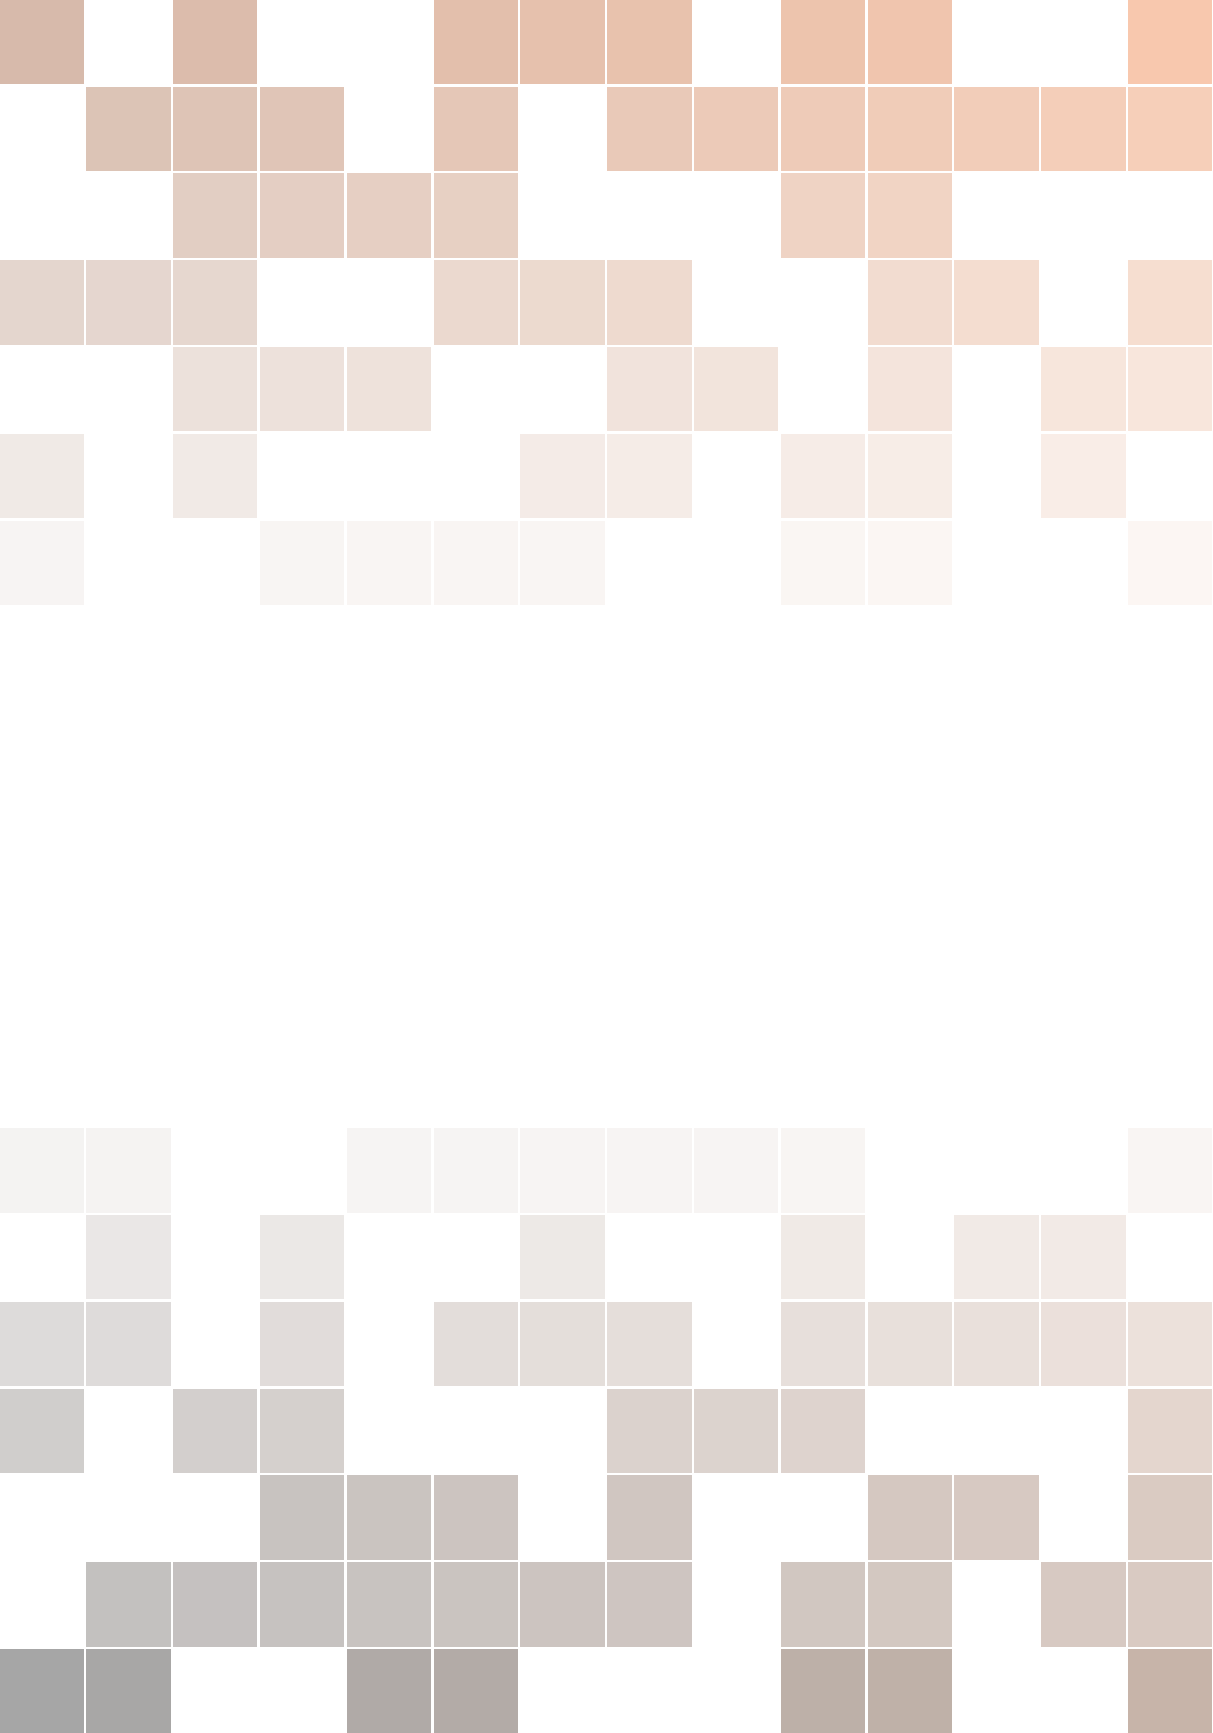
\includegraphics[width=\paperwidth]{images/background}}; % Background image
%\textsl{}
%      \draw[anchor=north] (midpoint) node [fill=ocre!30!white,fill opacity=0.6,text opacity=1,inner sep=1cm]{\Huge\centering\bfseries\sffamily\parbox[c][][t]{\paperwidth}{\centering Coding Interview Essentials\\[15pt] % Book title
%      {\Large - }\\[20pt] % Subtitle
%      {\huge Davide Spataro}}}; % Author name
%    \end{tikzpicture}};
%\end{tikzpicture}
%\vfill
%\endgroup


\includepdf[pages={2},fitpaper=true]{images/book_covers1.pdf}


\usechapterimagefalse % If you don't want to include a chapter image, use this to toggle images off - it can be enabled later with \usechapterimagetrue

%\chapterimage{images/header} % Table of contents heading image

\pagestyle{empty} % No headers

\tableofcontents % Print the table of contents itself

%\lstlistoflistings
%\listoffigures
%\listoftables

%\cleardoublepage % Forces the first chapter to start on an odd page so it's on the right

%pagestyle{fancy} % Print headers again


%!TEX root = ../main.tex
%%%%%%%%%%%%%%%%%%%%%%%%%%%%%%%%%%
% Links:
%
% Difficulty: Easy/Medium Companies: 
%%%%%%%%%%%%%%%%%%%%%%%%%%%%%%%%%%

%\chapterimage{header}

\chapter{Power set generation}
\label{ch:power_set}
\section*{Introduction}
The concept of power set is familiar to many because it is introduced very early during
introductionary math courses on set theory. The problem described in this chapter is about writing
an algorithm that is capable of finding the powerset of a given set. Two main solution approach are
presented here, one that is strightforward deriving immediately from the recursive definition of
power set\footnote{The following is the recursive definition of powerset. In words the powerset of an empty
set is a set contains as only element the empty set itself. For a non-empty set, let $e$ be an
element of the set and T be the original set minus $e$ (relative complement). The powerset can
be then definied as the union of two distinct powersets. The powerset of T (all the subsets not
containing $e$) and the powerset of T modified in a way such that $e$ is added to all of its
element.
\begin{equation}
	\mathcal{P}(S)=\begin{cases} 
\{\{\}\} & \text{if } P=\{\} \\
P\{T\} \bigcup \{t \in P\{T\} : t \cup \{e\}\} \text{ where } e \in P, \text{ and } T = P \setminus \{e\} & \text{otherwise}
\end{cases}
\label{eq:power_set_recursive_definition}
\end{equation} 
} (See Equation \ref{eq:power_set_recursive_definition}), while the other is based on a clever
observation about the distribution of the bits among the integers from $0$ to the size of the
powerset. The problem is usually presented in a very direct manner with a short and concise
statement because the interviewer is expecting the candidate to be already familiar with the
concept.



\section{Problem statement}
	\begin{exercise}
		Write a function that given a set of elements $P$ returns its power-set. A power-set of a set $P$,
		(here denoted as $\mathcal{P}(S)$ is the set of all its subsets including the empty subset
		$\emptyset$ and $P$ itself.

		\begin{example}
			\hfill \\
			For example, given the set $P=\{a,b,c\}$, the following two sets are both correct outputs for
			this problem:
			\begin{equation*}
				\{\{\}, \{b,c\}, \{a\}, \{a,b\}, \{a,b,c\}, \{b\}, \{a,c\}, \{c\} \}
			\end{equation*}
			\begin{equation*}
				\{\{\}, \{a\}, \{b\}, \{c\}, \{a,b\}, \{b,c\}, \{a,c\}, \{a,b,c\} \}
			\end{equation*}
			
		\end{example}
	\end{exercise}
\section{Clarification Questions}

\begin{QandA}
	\item What is the maximum size of the input?
	\begin{answered}
		\textit{The maximum number of element is strictly less than $n < 32$.}
	\end{answered}
	
	\item Are all the element in the collection distinct?
	\begin{answered}
		\textit{No, the elements are not necessarily distinct. $S$ can contain duplicates.}
	\end{answered}

	\item Can the subset in the power-set appear in any order?
	\begin{answered}
		\textit{Yes, subsets can appear in any order.}
	\end{answered}
\end{QandA}

\section{Discussion}
\label{sec:powerset:discussion}
There is one key point that should immediately be noticed: \textbf{The powerset of a collection of
	$n$ elements has size} $\boxed{2^n}$\footnote{The proof of this fact is relatively easy and it boils
	down to the fact that a subset of $P$ is basically $P$ with possibly some of the elements
	removed from it. Because we two possible choices we can make for every element of $S$ (either
	remove or not remove and element) then the total number of possible subset is: $2 \times 2
	\times \ldots \times 2 = 2^{|P|}$. Two choices for the first element, two for the second, and so
	on until the last element of $P$.} . This fact should be immediately pointed out during the
	interview, stressing the fact that the constraint $n < 32$ is a strong hint towards the fact
	that an exponential solution is expected. After-all we are required to output all the elements
	of the powerset, and thus the complexity of any algorithm solving this problem cannot be less
	than the size of the powerset itself. Doing so shows general knowledge on set theory and the
	ability to link and use that knowledge with the problem statement.


\subsection{Backtracking}
The first solution presented in this chapter is based on the fact that that during the generation of
one of the elements of the power-set a decision has to be taken for each element of the original
set, on whether to include the element or not into the subset. When a decision for the first element
is taken then what we are left with is $|P|-1$ decisions before we have created a valid subset of
$|P|$. 
This kind of process can be easily visualized with a tree where a node at level $i$
represents a decision for the $i^{th}$ element and a path from the root to a leaf uniquely
identifies a subset of $P$ i.e. $n$ decisions. 
All paths from the root to the leafs thus, represent the power set. In
order to solve this problem we have to explore the entirety of this tree. An example of such tree is
shown in Figure \ref{ref:power_set_decision_trees}.

One general way to deal with such type of problems is by using backtracking to try all possible
decision paths for each of the elements. The general idea is that we are going to, for all elements
starting from the first until the last, to explore the two possibilities: take or exclude the
element from the subset. Backtracking is a general algorithm that allows to enumerate and explore
large search spaces like this one. The main idea is that we first try to stick with a decision for
the first element, and we continue from there to generate all possible subsets where said decision
is never changed. When there is no more subset to generate, we backtrack and change our first
decisions to the next possible one and repeat the process of generating all possible subsets.
The proposed solution will incrementally construct one subset at the time, using an integer variable
to keep track of which element we are currently
deciding to include or exclude. The base case of the recursion happen when there is no more decision
to take, meaning that the current subset is ready to be included in the solution (it has been
produced after $n$ decision steps).

The C++ code implementing the idea above is shown in Listing \ref{list:power_set_backtracking}. The
complexity of this solution is exponential i.e. $O(2^n)$ which as already pointed out is as good as
it gets.


	\lstinputlisting[language=c++, caption="C++ to the power set generation using backtracking",label=list:power_set_backtracking]{sources/power_set/power_set_backtracking.cpp}


\begin{figure}
	\centering
	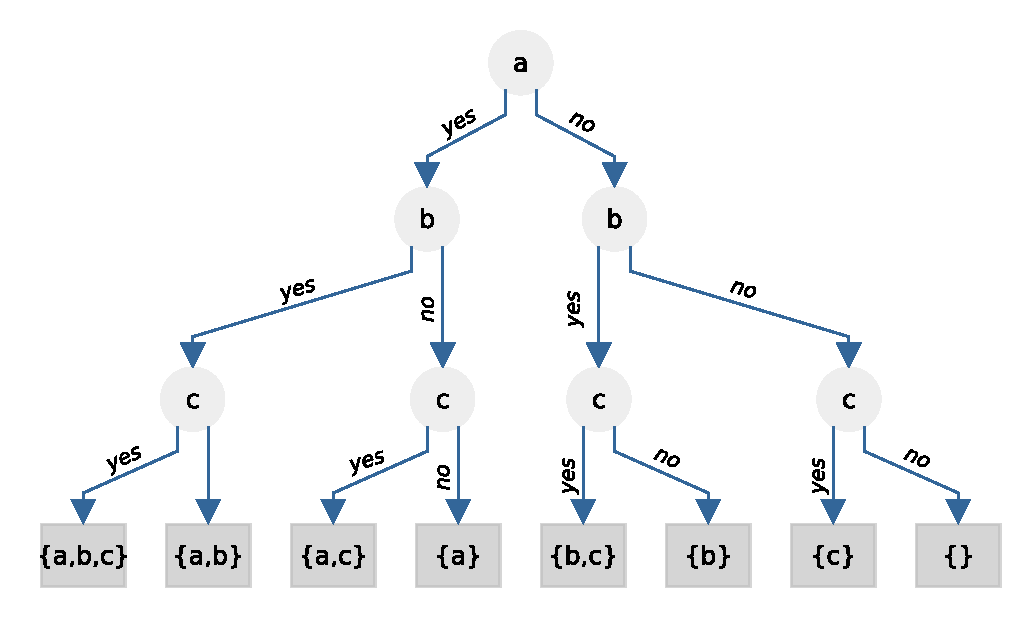
\includegraphics[width=\textwidth]{sources/power_set/images/tree}
	\caption[Decision tree for the power-set generation using backtracking.]{Decision tree for the power-set generation using backtracking. At level $i$ are the decision for the element $i$ in the original set. A labal marked with yes identifies the decision to take the corrensponding element into the subset, while a node labeled with no the opposite. At the last level is the powerset.}
	\label{ref:power_set_decision_trees}
\end{figure}

The advantages of using the backtracking framework to solve this problem is that, once we notice
that this problem can be solved by fully exploring the search tree, then we can immediately
start writing the code and rely on our experience as backtracking algorithm writers to implement a correct
solution with the added bonuses of being concise and short when written in a recusive form  as well
as well understood.
The downside is that the iterative implementation can be a little harder and more verbose to write.
Regardless of which one you choose, the interviewer is going to be pleased with your code provided you get to the final solution
without making too many implementation mistakes (forgetting to add the base case, or coding it wrong
is a pretty common one).

\subsection{Bit Manipulation}
Another approach that can be used to solve this problem is based on the fact that the values of the
bits of the numbers $\{0,1,2,\ldots, s^n-1\}$  already provide all the information necessary to make
the decision weather to include or not an element from the original set. 
The main idea is that the binary representation of the numbers from $0$ to $2^{n}-1$ is basically
the powerset of $n$ bits.
In other words, the binary representation of any of those numbers can be used to build one subset out
of the $n$ elements of the input set. 
For instance given the input $S=\{a,b,c\}$ the Table \ref{tab:mapping_value_bits} shows numbers from $0$ to $2^3-1 = 8$ and their bit
representation (second column) and how such information about which bit is set or not can be used to construct one
subset of the power-set of $P$ (third column). When the $i^{th}$ bit is set i.e. its value it $1$, it means that
corresponding $i^{th}$ element of $P$ is taken, while a non-set bit (with value $0$) means it is
excluded.

\begin{table}
	\centering
	\begin{tabular}{|l|l|l|}
		\hline
		Value & Bits & Subset\\ \hline
		0     & 000  & $\{\}$\\ \hline
		1     & 001  & $\{c\}$\\ \hline
		2     & 010  & $\{b\}$\\ \hline
		3     & 011  & $\{b,c\}$\\ \hline
		4     & 100  & $\{a\}$\\ \hline
		5     & 101  & $\{a,c\}$\\ \hline
		6     & 110  & $\{a,b\}$\\ \hline
		7     & 111  & $\{a,b,c\}$ \\ \hline
	\end{tabular}
	\caption[Mapping between bits and element of the powerset.]{This table shows a 1-to-1 mapping between integer values, their binary representation and an element of the powerset.}
	\label{tab:mapping_value_bits}
\end{table}

This idea can be used to write an algorithm in which all the numbers in the range $\{0,1,2,\ldots,
s^n-1\}$ are considered and each of them is used to generate a subset of the final solution.
Basically every number from such range maps uniquely to a subset of the powerset. It is really not
surprising when we think about the meaning of a bit in the binary representation of integers. One
can build a number by summing up powers of $2$ and the bits contains the information on whether a
certain power of two should be added to the final value for the represented number or not. With $n$
bits one can represents $2^n$ numbers, each corrensponding to one subset of the powerset of those
$n$ bits.

Listing \ref{list:power_set_bits} shows  a possible C++ implementation of the idea above\footnote{Notice the usage of the \texttt{reserve}
function that should be used in all those scenario when we already know the final size of the
collection we are building. This saves times because avoids intermediate allocation and copy that
must happen during the resize of the vector.}. The complexity of this implementation is, not
surprisingly, $O(2^n)$\footnote{Not considering the constant price of $32$ that we pay for each
subset generation due to the fact that we need to inspect the value of all of the bits}. Also please
pay attention to the fact that the proposed implementation assumes that the size of
\lstinline[columns=fixed]{int} is $4$ bytes, which is true for most architecture but not for all\cite{cit::std::fundamentaltypes}. A better
implementation would use \lstinline[columns=fixed]{std::numeric_limits<int>::digits} instead of
the magic number $32$.



	\lstinputlisting[language=c++, caption="C++ backtracking solution to the problem of generating the powerset.",label=list:power_set_bits]{sources/power_set/power_set_bit_manipulation.cpp}


%\section{Common variations}

%\section{Conclusion}

%!TEX root = ../main.tex
%%%%%%%%%%%%%%%%%%%%%%%%%%%%%%%%%%
% Links:
%
% Difficulty: Easy/Medium
% Companies: 
%%%%%%%%%%%%%%%%%%%%%%%%%%%%%%%%%%

\chapterimage{header}

\chapter{Square root of an integer}
\label{ch:square_root}
\section*{Introduction}
Calculation of the square root of an integer is a problem that is very often asked in coding interview question mostly because there exists a quite obvious solution that is not trivial to implement and a faster solution that works for larger input. It is a very good question to showcase implementation skills and algorithmic thinking.

\section{Problem statement}
Write a function (with signature: \lstinline[columns=fixed]{int my_sqrt(const int n)} ) calculates the square root of an integer rounded down to the nearest integer without using any library call.

\begin{example}
	\hfill \\
	\begin{itemize}
		\item[-] 	\lstinline[columns=fixed]{my_sqrt(9)=3}: $\Longleftarrow $ $\ceil{\sqrt{9}}=3$
		\item[-] 	\lstinline[columns=fixed]{my_sqrt(11)=3}: $\Longleftarrow $ $\ceil{\sqrt{11}}\approx\ceil{3.316624}=3$
		\item[-] 	\lstinline[columns=fixed]{my_sqrt(18)=4}: $\Longleftarrow $ $\ceil{\sqrt{11}}\approx\ceil{4.242640}=4$
	\end{itemize}

\end{example}

\section{Clarification Questions}

\begin{QandA}
	\item What is the maximum value the parameter $n$ can take?
	\begin{answered}
		\textit{The maximum number of element smaller than $2^{32}$.}
	\end{answered}
	
	\item Is $n$ guaranteed to be always positive?
	\begin{answered}
		\textit{Yes, there is no need to check for invalid input.}
	\end{answered}
\end{QandA}

\section{Discussion}
The interviewer is very likely expecting to see a brute force solution appear on the whiteboard within the first 5-7 minutes. The reason is that the brute force approach for this problem is quite easy conceptually but its implementation in a concise manner requires some thinking. 

\subsection{Brute-Force}
The square root of a number can be found by testing all numbers from $k=0,1,2,\ldots$ until a solution is found i.e. $k^2\leq n$ and $(k+1)(k+1) > n$ . A solution is guaranteed to be found, and it should be immediately noticed that no more than $\sqrt{n}$ numbers will be tested. Therefore the time complexity of this approach is $O(\sqrt{n})$.
Listing \ref{list:square_root_brute_force} shows a possible implementation. Note that the variable $i$ has a type in C++ that is larger in size than $int$. This prevents overflows during the calculation of $i^2$ in the while condition if the input $n=2^{32}$.

\begin{minipage}{\linewidth}
	\lstinputlisting[language=c++, caption=$O(\sqrt{n})$ solution to the problem of finding the square root of an integer.,label=list:square_root_brute_force]{sources/square_root/square_root_brute_force.cpp}
\end{minipage}

\subsection{Logarithmic Solution}
Binary search can be effectively used to solve this problem. In order to show that, it is beneficial to look at the problem from a slightly different angle. 
Let 
\begin{equation}
	F(k)=\begin{cases} 
0 & k^2 \leq n \\
1 & k^2 > n
\end{cases}
\label{eq:square_root_piecewice}
\end{equation} 
be a piece-wise function that partition the search space $[0\ldots n]$ into two sets (See Table \ref{tab:sqrt_split_space}):
	\begin{itemize}
      \item [-] the numbers  less or equal than $\sqrt{n}$
      \item [-] the numbers strictly greater or equal than $\sqrt{n}$
	\end{itemize}

\begin{table}[]
	\centering
	\begin{tabular}{|c|c|c|c|c|c|c|}
		\hline
		$0$ & $1$ & $2$   & $\sqrt{n}$ & $\sqrt{n}+1$ & \ldots   & $n$ \\ \hline
		$0$ & $0$ & \ldots & $1$ & $1$ & \ldots & $1$   \\ \hline
	\end{tabular}
\label{tab:sqrt_split_space}
\caption{Partition of the search space according to the function in Eq. \ref{eq:square_root_piecewice}}
\end{table}
What the function should return is basically the greatest $k$ s.t. $F(k)=0$. 

Because of the peculiarity of the function $F(k)$ i.e. (divided into two partition) we can use binary search to find the end of the first partition as shown in Listing \ref{list:square_root_binary_search}. Note how a the algorithm works by iteratively searching in a smaller subinterval defined by the variables $l$ and $r$. At each iteration test the middle element of the subinterval (variable $middle$), and this can lead to three scenarios:

\begin{enumerate}
 	\item $(middle)^2  = n \longrightarrow$. $middle$ is the solution. $n$ is a perfect square and $\sqrt(n)=middle$
 	\item $(middle)^2  > n \longrightarrow$. $middle$ is not the solution and we can also exclude all numbers $k \geq middle$ (by doing $r = middle-1$).
 	\item $(middle)^2  < n \longrightarrow$. $middle$ is the best guess we have found so far. we can also exclude all numbers $k < middle$ from the next iterations (by doing $l = middle+1$).
\end{enumerate}
As a bonus it might be also good to point out to the interviewer the fact that the middle element is not calculated as it is commonly done i.e. $(l+r)/2$ in order to prevent overflow when $l+r$ is calculated.

\begin{minipage}{\linewidth}

	\lstinputlisting[language=c++, caption=$O(log_2(n))$ solution to the problem of finding the square root of an integer.,label=list:square_root_binary_search]{sources/square_root/square_root_binary_search.cpp}
\end{minipage}

Not surprisingly the complexity of this solution is logarithmic.


\section{Conclusion}

%!TEX root = ../main.tex
%%%%%%%%%%%%%%%%%%%%%%%%%%%%%%%%%%
% Links:
%
% Difficulty: Easy/Medium Companies: 
%%%%%%%%%%%%%%%%%%%%%%%%%%%%%%%%%%

\chapterimage{header}

\chapter{Two string anagram}
\label{ch:two_string_anagram}
\section*{Introduction}
From a set of words, you can construct other words by only changing the arrangements of their characters.
For instance, from the characters in \textit{"alerting"} you can spell the following words:
\begin{itemize}
	\item  \textit{"altering"}
	\item  \textit{"integral"}
	\item  \textit{"relating"}
	\item  \textit{"triangle"}.
\end{itemize}
Words sharing the same characters set are called \textbf{anagrams}. 

Being able to create good anagrams, especially if they are able to reflect or comments on the words they are generated from (for instance turning
\textit{"Madam Curie"} into \textit{"Radium came"}) is regarded as a rather difficult task.
Computers have been used for a long time to find anagrams in long texts, as well as to generate the so-called anagram dictionaries.  A special kind of dictionary, where all the letters in a word and
all their transposition are arranged in alphabetical order,  are often used in games like
Scrabble\footnote{https://en.wikipedia.org/wiki/Scrabble}. Often, at the core of such applications lies an efficient algorithm for determining if a word is an anagram of another word.

As it is pretty clear at this point, the problem discussed in this lesson is about anagrams, and more specifically, about determining the number of
modifications you need to make to a word in order to make it a valid anagram of a
another word.
This kind of question is considered rather easy during a coding interview process, as it does not require particular insights or particularly tricky reasoning in order to come up with an efficient solution, aside from understanding the concept of an anagram, which is common knowledge.

That said, it is still very much worth studying this problem as it is frequently asked during the preliminary interview stages. Moreover, despite its simplicity, there is more than one neat and elegant approach leading to an efficient
solution to this problem.

In the rest of the chapter we are going to have a look at three
solutions, starting from the slow but easy to understand brute-force in Section \ref{sec:anagrams:bruteforce} then touching briefly on a faster approach using sorting in Section \ref{sec:anagrams:sorting},and finally, and finally, we will get to the optimal solution running in linear time in Section
\ref{sec:anagrams:histograms}. 

\section{Problem statement}
	\begin{exercise}
		Write a function that given two string, $a$ and $b$ of length $n$ and $m$, respectively, determines the minimum number of character substitution, $C(s, i, c)$, necessary to make the string $a$ an anagram of the string $b$.

		Two strings are said to be anagrams of one another if you can turn the first string into the second by rearranging its letters. 

		A substitution operation $C(s,i,c)$ modifies the string $s$, by changing its $i^{th}$ character into $c$. Notice that deletions or additions of characters are not allowed.
		The only operation you can do is change a character of the first string into another one. 

		In other words, what is the minimum number of characters of the input strings that need to be modified (no addition or deletion)  so that $a$ becomes an anagram of $b$?
		
	\begin{example}
		\label{ex:two_string_anagram:example1}
		\hfill \\
		\begin{itemize}
			\item 	a = "aaa"
			\item 	b = "bbb"
		\end{itemize}
		The function returns $3$. 
		All the characters of \textit{a} need to be changed into \textit{'b'}.
		\label{ex:anagrams:example1}
	\end{example}

	\begin{example}
		\hfill \\
		\begin{itemize}
			\item 	a = "tear"
			\item	b = "fear"
		\end{itemize}
		The function returns $1$. 
		All it is necessary is turning the first letter \textit{'t'} into a \textit{'f'}.
	\end{example}

	\begin{example}
		\hfill \\
		\begin{itemize}
			\item[] 	a = "Protectional"
			\item[] 	b = "Lactoprotein"
		\end{itemize}
		The answer for this case is $0$ because \emph{Protectional} is already an angram of \emph{Lactoprotein}.
	\end{example}
\end{exercise}

\section{Clarification Questions}

\begin{QandA}
	\item \begin{questionitem} \begin{question} Are the letters of the string always only letters from the English alphabet?    \end{question}      
    \begin{answered}
		\textit{Yes, letters are always from the English alphabet.}
	\end{answered} \end{questionitem}
	
	\item \begin{questionitem} \begin{question} Should the function be case sensitive?   \end{question}      
    \begin{answered}
		\textit{ No. You can assume the input letters are always lower case.}
	\end{answered} \end{questionitem}
	\item \begin{questionitem} \begin{question} Can the input string be modified? No, the input is immutable.  \end{question}      
    \begin{answered}
		\textit{No, the input strings are immutable.}
	\end{answered} \end{questionitem}

	\item \begin{questionitem} \begin{question} What value should be returned when there is no solution?  \end{question}      
    \begin{answered}
		\textit{In such case you can return $-1$.}
	\end{answered} \end{questionitem}
\end{QandA}

\section{Discussion}

Let's start by first quickly review what the word anagram means in the context of this problem. First of all, notice that both $a$ and $b$ contain a single word (which can be fairly long).
Moreover, for $a$ to be an anagram
of $b$, it has to be the case that exists an arrangement of characters in $a$ that is equal to $b$.
In other words, the question to which we need to answer is: is it possible to shuffle the character of $a$ such that we obtain $b$?
For this to be the case, it must be that $a$ and $b$ contain the same set of characters meaning that sorting both $a$ and $b$ would make them equal.
In addition, as a consequence of the fact that no addition or deletion
is allowed, \textbf{$a$ and $b$ must have the same length}. 
On the other hand, if they have the same length then it is always
possible to solve this problem because in the worst case, we can modify every letter of $a$ (see Example \ref{ex:two_string_anagram:example1}).
Thus, the only case when the problem has no solution has been isolated: when $n \neq m$ we must return $-1$ otherwise we can proceed with our calculation knowing that a solution exists.

\subsection{Brute-Force}
\label{sec:anagrams:bruteforce}
One of the first options coming to mind is a solution where we generate all possible arrangements of the letters in $a$, and for each of these arrangements, calculate the number of modifications necessary to convert it into $b$. 
The key idea is that the cost of transforming a string into another is equal to the number positions having different letters. 
For instance, the cost of transforming \textit{"abcb"} into \textit{"bbbb"} is $2$ because the two strings differ in the first and third letters. 

Although it is simple to explain, this approach must be considered poor because the number of arrangements of a set of $n$ letters grows as fast as $n!$.
Moreover, enumerating all the arrangements is no trivial task, unless we use a  library function capable of doing that (for instance, the C++ standard library provides the function \inline{std::next_permutation}\footnote{\href{https://en.cppreference.com/w/cpp/algorithm/next_permutation}{https://en.cppreference.com/w/cpp/algorithm/next\_permutation}} devoted to this purpose).


Listings \ref{list:two_string_anagram_bruteforce} shows a C++ implementation of the idea above.

\lstinputlisting[language=c++, caption="Brute force.",label=list:two_string_anagram_bruteforce]{sources/two_string_anagram/two_string_anagram_brute_force.cpp}


\subsection{Sorting}
\label{sec:anagrams:sorting}
The brute-force solution does a lot of superfluous work, because it tries to find a permutation of the string $a$ requiring minimal modifications to be morphed into $b$.
But is it really necessary to turn $a$ into \textbf{exactly} $b$, or is it sufficient to modify $a$ so that it is equal to a particular permutation of $b$? 
After all, being an anagram is a transitive property: if $a$ is a permutation of $b$ and $b$ is a permutation of $c$, then $a$ must also be a permutation of $c$. 

By definition, an anagram of $b$ is any permutation of its characters, and therefore, the particular permutation in which the characters of $b$ are sorted is a valid anagram on its own. 
It is much easier than checking all possible permutations, to modify $a$ into the "sorted" anagram of $b$ (where all of its characters are sorted), rather than to exactly $b$ because all we need to do is to create a copy of both $a$ and $b$, sort both of them and then calculate the character-by-character difference.
\textbf{This approach works because if $x$ is an anagram of $b$ then $x$ is also an
anagram of `sort(b)`}.
In other words, it does not matter how the characters are arranged in $a$ and $b$, as the only thing that matters is the set of the characters
appearing in $a$ and $b$: the order in which characters in both $a$ and $b$ appear does not matter. 

Listings \ref{list:two_string_anagram_sorting}  shows how we can take advantage of this fact and write a fast solution for this problem.

\lstinputlisting[language=c++, caption="Solution based on sorting.",label=list:two_string_anagram_sorting]{sources/two_string_anagram/two_string_anagram_sorting.cpp}

Notice that, if the input was mutable, then, the additional space occupied by the copies of the string \inline{aa} and \inline{bb} could have been avoided. 

The time complexity of Listing \ref{list:two_string_anagram_sorting}  is $O(n log(n))$ (because of sorting). The space complexity is $O(n)$ (we create copies of the input strings).



\subsection{Histograms}
\label{sec:anagrams:histograms}


There is another bit of information that we have not used yet: \textbf{the alphabet} from which the
letters of $a$ and $ab$ are taken from \textbf{is small}. 
If the only thing that matters is the set of characters appearing in $a$ and $b$ (and not their order, as discussed above),
then we can use the same idea at the core of the \href{https://en.wikipedia.org/wiki/Bucket_sort}{bucket sort} algorithm to achieve a linear time complexity solution.


The key idea is to pre-process $a$ and $b$ so to calculate their per-character frequencies, denoted here as $F_a$ and $F_b$, respectively.
An entry of $F_a[\mathrm{c}]$ and $F_b[\mathrm{c}]$, where $\mathrm{c} \in \{\mathrm{a},\mathrm{b},\ldots,\mathrm{z}\}$ (a letter of the alphabet), contains the frequency of character $\mathrm{c}$, in $a$ and $b$, respectively.


If $F_a$ and $F_b$ are the same, then $a$ and $b$ have exactly the same character set and $a$ is an anagram of $b$.
Otherwise, it must be the case that some characters of $a$ appear in $b$ a different number of times.
In this case, we can fix $a$ in such a way to make sure that its frequencies $F_a$ ey match the ones in $F_b$. 
But the main question is still unanswered: how many operations are necessary to do so?  In order to get this answer, it is useful to look at
the difference ($D$) of $F_a$ and $F_b$.

$D = F_a - F_b = \{D[\mathrm{a}] = (F_a[\mathrm{a}] - F_b[\mathrm{a}]), D[\mathrm{b}] = (F_a[\mathrm{b}] - F_b[\mathrm{b}]), D[\mathrm{c}] = (F_a[\mathrm{c}] - F_b[\mathrm{c}]), \ldots, D[\mathrm{z}] = (F_a[\mathrm{z}] - F_b[\mathrm{z}])\}
$

$D[\mathrm{c}]$ (where $\mathrm{c} \in \{\mathrm{a},\mathrm{b},\ldots,\mathrm{z}\}$) contains the difference between the number of occurrences of the character $\mathrm{c}$ in the string $a$ and $b$. Depending on whether the value of $D[\mathrm{c}]$  is greater or smaller than $0$, $a$ has an excess or a deficit of the letter c, respectively.

Firstly, notice that $\sum_{c=\mathrm{a}}^{\mathrm{z}} D[\mathrm{c}] = 0$. This observation stems from the fact that $|a|=n=m=|b|$ ($a$ and $b$ must have equal length for this problem to have a solution, remember?) and that if $a$ has an excess of a certain character $\mathrm{c}$ then there must exist another character $\mathrm{d} \neq \mathrm{c}$ that the string $a$ has a shortage of. If that is not the case, it is impossible for $a$ and $b$ to have equal length.

We can use this fact to modify the excesses of the letters of $a$, the ones having a positive value of $D$ into some of the letters there is a shortage of so that eventually, every single value of $D$ is zero.
If $D[\mathrm{c}] = x$ is going to take $x$ modifications to transform the excess of characters $\mathrm{c}$.
The answer to this problem is, therefore, the sum of all the positive numbers of $D$. 

Listings \ref{list:two_string_anagram_histogram} shows a possible implemenetation of the idea above.

\lstinputlisting[language=c++, caption="C++ solution to the two string anagram problem using the histogram approach.",label=list:two_string_anagram_histogram]{sources/two_string_anagram/two_string_anagram_histogram.cpp}

Notice how the array of differences of frequencies $D$ can be easily calculated without explicitly
computing the frequencies for the characters of $a$ and $b$ but by simply adding $1$ to $D[\mathrm{c}]$ when the letter $\mathrm{c}$ appears in $a$
and subtracting $1$ when it does in $b$. 

The time and space complexity of the code above is $O(n)$ and $O(1)$ in space (we are using an array of $128$ integers regardless of the size of the input). We cannot do any better than this, as all characters in the input strings must be at least read once.



%\section{Conclusion}

%!TEX root = ../main.tex
%%%%%%%%%%%%%%%%%%%%%%%%%%%%%%%%%%
% Links: https://www.geeksforgeeks.org/count-pairs-with-given-sum/
% https://algorithms.tutorialhorizon.com/given-an-array-and-a-number-k-check-for-pair-in-array-with-sum-as-k-in-onlgn/
% https://coderbyte.com/algorithm/two-sum-problem https://en.wikipedia.org/wiki/Subset_sum_problem
%
% Difficulty: Easy Companies: Microsoft, Amazon, Google
%%%%%%%%%%%%%%%%%%%%%%%%%%%%%%%%%%

\chapterimage{header} % Table of contents heading image

\chapter{Two numbers sum problem}
\label{ch:two_numbers_sum}
\section*{Introduction}
The problem described in this lesson is probably one of the most asked during coding interviews nowadays, mostly 
during the early online stages of the hiring process: the interviewer pretty much expects a candidate to be at least familiar with the problem or to have read it at some point during his preparation.

The problem is hard enough to require non-trivial insights in order to be able to write a non-trivial solution but, at the same time, it is not so hard that it would take you hours to come up with something meaningful to say or to write.

We will have a look at a number of solutions: First, we will start from the inefficient brute force approach (and we will later refine it into a fast and time-optimal one);
Then we will delve also into a radically different approach based on sorting; finally, we will condense the strengths of all the solutions investigated so far into a time and space optimal solution that we think would do better in an interview context. As we will see, the final solution is efficient and not terribly difficult to write and explain (which are fundamental aspects of every successful coding interview).


\section{Problem statement}

\begin{exercise}
	Write a function that takes an array of integers $A$ of size $n$ and an integer $T$, and returns \textbf{true} if the sum of any two distinct elements $I$ is equal to $T$, \textbf{false} otherwise.

	More formally: Given an array $=\{a_1,...,a_n\}$ and $T$, where $a_i, T \in
	\mathcal{N}$, return:
	\begin{itemize}
		\item  \textbf{true} if $\: \exists \;i,j \:\: i \neq j$ s.t. $a_i+a_j = T$
		\item  \textbf{false} otherwise
	\end{itemize}
	

	\begin{example}
	\hfill \\
		Given $A=\{9, 4, 17, 42, 36, -3 ,15\}$ and $T=14$, the function returns \textbf{true} because we can obtain $14$ by summing
		up together the elements $17$ and $-3$.
		If $T=17$ the answer is \textbf{false}.
	\end{example}

	\begin{example}
	\hfill \\
		Given $A=\{1,3,7\}$ and $T=8$, the function returns \textbf{true} because we can obtain $8$ by summing
		up together the elements $7$ and $1$. If $T=6$ the answer is \textbf{false}.
	\end{example}

\end{exercise}	


\section{Clarification Questions}
\begin{QandA}
	\item \begin{questionitem} \begin{question} Is the input array modifiable?  \end{question} 	 
    \begin{answered}
		\textit{Yes, the input array can be modified.}
	\end{answered} \end{questionitem}	
	\item \begin{questionitem} \begin{question} Are the integers guaranteed to be all positive or all negative?   \end{question} 	 
    \begin{answered}
		\textit{No, $A$ can contain positive or negative numbers.}
	\end{answered} \end{questionitem}
	\item \begin{questionitem} \begin{question} Are the values in $A$ guaranteed to be from a given range?  \end{question} 	 
    \begin{answered}
		\textit{No, the input is arbitrary. No assumption can be made on the magnitude of the elements of $A$.}
	\end{answered} \end{questionitem}
	\item \begin{questionitem} \begin{question} Can a pair be made from an element and itself?  \end{question} 	 
    \begin{answered}
		\textit{No, the pair's elements should be distinct. You cannot use the same element $a_i$ twice. You can however use two elements at indices $i$ and $j$ s.t. $i \neq j$ and $a_i=a_j$.}
	\end{answered} \end{questionitem}
	\item \begin{questionitem} \begin{question} Are all elements in the array unique?  \end{question} 	 
    \begin{answered}
		\textit{No, duplicates are allowed.}
	\end{answered} \end{questionitem}
	\item \begin{questionitem} \begin{question} Is the input sorted?  \end{question} 	 
    \begin{answered}
		\textit{No, the ordering of $A$ is arbitrary.}
	\end{answered} \end{questionitem}
	\item \begin{questionitem} \begin{question} Shall the function integer overflow be considered when performing the sum of two integers? Is it possible for two elements of $A$ to sum up to a value that does not fit in a standard \inline{int}?  \end{question} 	 
    \begin{answered}
		\textit{No, you do not need to worry about overflow.}
	\end{answered} \end{questionitem}
\end{QandA}


\section{Discussion}

%%%%%%%%%%%%%%%%%%%%%%%%%%%%%%%%%%%%%%%
%        quadratic solution
%%%%%%%%%%%%%%%%%%%%%%%%%%%%%%%%%%%%%%
\subsection{Brute-force}
\label{sec:two_numbers:bruteforce}

The brute force solution is fairly straightforward because it consists of a direct application of the formal problem statement. 
The solution space consists of all possible ordered pairs $(a_i,a_j)$, $i < j$. 
Two nested loops can be used to enumerate all those pairs, and, for each of them, we can check whether their sum is equal to $T$: if that is the case,
then   \textbf{true} can be immediately returned, otherwise, if we have checked every possible pair and none of them was good, then we can return  \textbf{false}.
You will find an a fomalization and an implementation of this idea in Algorithm \ref{algo:two_number_sum_bruteforce}
and Listing \ref{list:two_number_sum_bruteforce}), respectively.

\begin{algorithm}
	\SetAlgoLined \SetKwFunction{FMain}{solveQuadratic}
	
	\KwIn{$ A $ \tcp{An array $A$ of length $n$}} \KwIn{$ T $ \tcp{An integer $T$}}

	\Fn{\FMain{$A,T$}}{
	
		%\Output{true if two distinct element of $A$ sum to $T$}
		
		\For{$i\leftarrow 0$ \KwTo $n-1$} {\For{$j\leftarrow i+1$ \KwTo $n$} {\If{$a_i + a_j =
		T$}{\Return True \;}}} \Return False \;}\textbf{End Function}
	
		\caption{Two loops, quadratic solution to the question in Section \ref{ch:two_numbers_sum} }
		\label{algo:two_number_sum_bruteforce}
\end{algorithm}


\lstinputlisting[language=c++, caption="C++ solution of the two number sum problem with a brute force approach.",label=list:two_number_sum_bruteforce]{sources/two_numbers_sum/brute_force.cpp}

The time complexity of this solution is $O(n^2)$ because there is a quadratic number of
ordered pairs and in the worst case, we will look at \textbf{all} of them.

The number of iterations of the internal loop depends on the value of $i$ and
it is described by the function: $f(i) = n-i-1$. The total number of iteration the second
loop runs in the worst case is the the sum of $f(i)$ for all values of $i$: 
$\sum_{i=0}^{n-2} f(i) = (n-1) + (n-2) + (n-3) \ldots + 1 =\sum_{x=1}^{n-1} x= \frac{n(n-1)}{2} = O(n^2)$

The space complexity is $O(1)$.



\subsection{Hashing}
\label{sec:two_numbers:hashing}
The internal loop of the brute force solution above can be eliminated entirely with the help of a hash table.
The key insight is that if a solution exists involving $a_i$ then, it must the case that exists another element $a_j  = a_i-T$ with $i > j$. 

What this means in practice is that we can loop through $A$ one element at a time and keep track, in a lookup table, of all the elements seen so far, so that the lookup operation for the aforementioned element $a_j$ can be performed in constant time.

Algorithm \ref{algo:two_number_sum_hashset} and Listing \ref{list:two_number_sum_hashing} shows this idea in code.

%%%%%%%%%%%%%%%%%%%%%%%%%%%%%%%%%%%%%%%
% two_numbers_sum_hashset       
%%%%%%%%%%%%%%%%%%%%%%%%%%%%%%%%%%%%%%
\begin{algorithm}
	%	\KwData{} \KwResult{Tr }
	\KwIn{$ A $ \tcp{An array $A$ of length $n$}} \KwIn{$ T $ \tcp{An integer $T$}} \KwOut{true if
	two distinct element of $A$ sum to $T$, False otherwise} \SetKwFunction{FMain}{solveHashSet}
	
    \Fn{\FMain{$A,T$}}{H $\longleftarrow$ \CreateHashSet \;
	
		\For{$i\leftarrow 0$ \KwTo $n$} {target $\leftarrow$ $(T-a_i)$ \eIf{H.find(target)} {\Return
		True} {H.insert($a_i$)}} \Return False\;}\textbf{End Function}

		\caption{Hashset, linear solution to the \textit{two number sum} question in Section
		\ref{ch:two_numbers_sum}.}
		\label{algo:two_number_sum_hashset}
\end{algorithm}


\lstinputlisting[language=c++, caption="C++ solution of the two number sum problem using hashing.",label=list:two_number_sum_hashing]{sources/two_numbers_sum/hashset.cpp}

The time complexity of this approach is $O(n)$ (technically is linear on average due to complexity of lookups in hash tables) because the input array is scanned once and for each
of its elements, only one lookup and insertion are performed in the hash table (both operations costing constant time on average).

The space complexity
is also $O(n)$, as in the worst case the whole input array is stored in the lookup table.

A common mistake when solving this problem using this approach is to insert the whole input array into the lookup table, and only after searching for $(T-a_i)$.
The mistake becomes evident when $T$ is an even number ($2 | T$) and $\frac{T}{2}$ appears in $A$  exactly once, at index $k$ i.e. $a_k = \frac{T}{2}$ causing \inline{H.find(T-a_k)} to return \textbf{true}, which is wrong because this corresponds to a solution where we sum $a_k$ twice to obtain $T$.

For instance, when $A=\{1,2,5,4\}$ and $T=10$ this approach wrongly returns \textbf{true}, even if there are not two elements at distinct indices in $A$ whose sum is $T$ (we would use $5$ twice to obtain $10$).
\begin{example}
	\hfill \\ 
	\begin{itemize}
		\item[] $A=\{1,2,5,4\}$
	\item[] $T = 10$
\end{itemize}
	Algorithm \ref{algo:two_numbers_sum_hashset_wrong} wrongly return true even if there are not two
	distinct elements whose sum is $10$.
\end{example}


%%%%%%%%%%%%%%%%%%%%%%%%%%%%%%%%%%%%%%%
% two_numbers_sum_hashset_wrong       
%%%%%%%%%%%%%%%%%%%%%%%%%%%%%%%%%%%%%%
\begin{algorithm}
	\SetKwInOut{Input}{input} \SetKwInOut{Output}{output}
	\SetKwFunction{CreateHashSet}{CreateHashSet<int>} \Input{An array $A$ of length $n$} \Input{An
	integer $T$} \Output{true if two distinct element of $A$ sum to $T$}
	
	\SetKwFunction{FMain}{solveHashSet} \Fn{\FMain{$A,T$}}{H $\longleftarrow$ \CreateHashSet \;
		\tcp{Add the whole array in the hashset}
		\For{$i\leftarrow 0$ \KwTo $n$} {H.insert($a_i$)\;}
		
		\For{$i\leftarrow 0$ \KwTo $n$} {target $\leftarrow$ $T-a_i$ \; \If{H.find(target)} {\Return
		True}} \Return False\;}\textbf{End Function}
		\caption{Hashset, linear solution to the \textit{two number sum} question in Section
		\label{algo:two_numbers_sum_hashset_wrong}
	\ref{ch:two_numbers_sum} }
\end{algorithm}


\subsection{Sorting and binary search}
\label{sect:two_number_problem_binary_search}

As with countless other problems on arrays, sorting the input often opens the
way to a faster and more efficient solution. 

We can start by asking ourselves how the problem changes if  $A$ is sorted. Sorted arrays are naturally associated with binary search, and for good reasons! Many problems can be solved efficiently by pairing sorting and binary search on arrays. 
This problem is not different, and we can use binary search if $A$ is sorted to substitute the internal loop of the brute force solution presented [above](). This way, we can  lower the overall complexity down to $O(n log(n))$; it costs
$O(n log(n))$ to sort the input array in the first place, and the actual search consists of $n$ binary
searches, each of them costing $O(log(n))$. 

The space complexity is $O(1)$ because no additional space is required, since the array is sorted in place.

Listing \ref{list:two_number_sum_sorting} shows a C++ implementation of this idea. Notice that it uses \inline{std::binary_search} from the C++ standard library and that a possible follow-up question might be to show your own version of the binary search algorithm.



\lstinputlisting[language=c++, caption="C++ solution of the two number sum problem with sorting and binary search.",label=list:two_number_sum_sorting]{sources/two_numbers_sum/two_numbers_sum_sorting.cpp}


\subsection{Sorting and two pointers technique}
\label{sec:two_numbers:twopointers}

There is a variation to the to the approach described in Section
\ref{sect:two_number_problem_binary_search} which still involves sorting but uses a two-pointers
technique instead of binary search to finish the job. 

The key idea is that once $A$ is sorted, the algorithm initializes
two pointers, one starting at the beginning ($p_s$) and the other at the end ($p_e$) of the array, respectively.
It continues by looking at the sum of the two elements pointed by the two pointers and moving one of
the two at each step using the following logic: 
\begin{itemize}
	\item if $a[p_s]+a[p_e] = T$ a solution has been found. The algorithm returns true.
	\item if $a[p_s]+a[p_e] > T$, $p_e=p_e-1$. The right pointer is moved to the left. 
	Moving	$p_e$ to the left has the effect of making the sum of the values pointed by the two pointers smaller (this has an effect at the next iteration). 
	\item if $a[p_s]+a[p_e] < T$, $p_s=p_s+1$. The right end pointer is moved to the left. Moving $p_s$ to the right has the effect of making the sum of the values pointed by the two pointers larger. 
\end{itemize}



Listing \ref{list:two_number_sum_two_pointers} shows an implementation of the idea above. Notice that compared to the solution using the binary search, this one is shorter and simpler to write. Moreover, it does not use library functions. 

\lstinputlisting[language=c++, caption="C++ solution of the two number sum problem with the two pointers tecnique.",label=list:two_number_sum_two_pointers]{sources/two_numbers_sum/two_numbers_sum_two_pointers.cpp}

Despite the overall time complexity is still $O(n log(n))$, this solution is likely to be faster than
the one using binary search, mostly due to the fact that the array is scanned linearly (which makes caches happier) by the two pointers and not in a scattered way as in the case of binary search.

%%%%%%%%%%%%%%%%%%%%%
\section{Common Variations}
\subsection{Four numbers sum problem}
\label{sec:four_number}

\subsection{Problem statement}

\begin{exercise}
Write a function that takes four arrays of integers, $A,B,C,D$ and a integer $T$,
and returns how many distinct tuple $(i,j,k,l)$ where exist such that $A_i+B_j+C_k+D_l = Y$.

\begin{example}
\hfill \\
Given:
	\begin{itemize}
		\item[-] 	$A=\{1,2\}$,
		\item[-] 	$B=\{-2,-1\}$,
		\item[-] 	$C=\{-1,2\}$,
		\item[-]	$D=\{0,2\}$, and 
		\item[-] 	$T = 0$
	\end{itemize}
The answer is $2$ because the only two valid tuples are:
\begin{enumerate}
	\item $(0,0,0,1)$: $A_0 + B_0 + C_0 + D_1 = 1 + (-2) + (-1) + 2 = T = 0$
	\item $(1,1,0,0)$: $A_1 + B_1 + C_0 + D_0 = 2 + (-1) + (-1) + (-1) = T = 0$
\end{enumerate}
\end{example}
\end{exercise}

\subsection{Na\"ive $O(n^4)$ solution}
We can solve this problem very easily by using the same approach we have described in Section \ref{sec:two_numbers:bruteforce}.
The idea is that we can use four nested loops and enumerate all possible 4-elements tuples of indices. Listing \ref{list:two_number_sum_naive} shows how such an idea can be implemented.
Goes without saying, that this is not the fastest solution we can come up with, considering it has a time complexity of $O(n^4)$

\lstinputlisting[language=c++, caption="Brute force na\"ive solution to the four numbers sum problem.",label=list:two_number_sum_naive]{sources/two_numbers_sum/variations/four_number_sum/four_number_sum_solution1.cpp}

Needless to say, that this is not the fastest solution we can come up with, considering it has a time complexity of $O(n^4)$.

\subsection{$O(n^3)$ solution}
The trivial solution shown in Listing \ref{list:two_number_sum_naive} can be improved by using a similar reason that lead us improve the brute-force 
quadratic time solution for the two numbers problem in Listing \ref{list:two_number_sum_bruteforce} to the linear time (and space) in Listing \ref{list:two_number_sum_hashing}.

The idea is that inner-most loop is searching for a value $D_l = x$  s.t. if it summed to $A_i+B_j+C_k$ gives us $T$; in other words: $x+(A_i+B_j+C_k)=T$.
Therefore $x = T-(A_i+B_j+C_k)$. If there is a way of avoiding a linear search in the array $D$ for such a value, then we could bring down the complexity from $O(n^4)$ to $O(n^3)$.

Thankfully, this is possible if we use a hash map. If we create a hashmap mapping the value of $D$ and to their frequencies, the inner-most loop of the $O(n^4)$ solution above can be substituted with a query to the hashmap which runs in constant time (on average). 

Listing \ref{list:two_number_sum_cubic} shows an implementation of such idea. 
Notice that, in order to obtain the maximum saving in terms of work avoided, the arrays are rearranged in such a way so that $D$ is the longest of the four input arrays. 

\lstinputlisting[language=c++, caption="Brute force cubic time solution to the four numbers sum problem.",label=list:two_number_sum_cubic]{sources/two_numbers_sum/variations/four_number_sum/four_number_sum_solution2.cpp}


\subsection{$O(n^2)$ solution using hashing}

This problem can be however be solved in quadratic time if we use hashmaps in a smarter way, to hold 
the frequencies of all the values we can obtain by summing up any two elements of $A$ and $B$ and of $C$ and $D$.
The key idea is that we can build two distinct hashmaps:
\begin{itemize}
	\item $AB$: holding the frequencies of the values obtainable by summing any two elements of $A$ and $B$
	\item $CD$: holding the frequencies of the values obtainable by summing any two elements of $C$ and $D$.
\end{itemize}

The space required for both $AB$ and $CD$ is quadratic, which is more than the space used by any of the previous solutions, but this extra space
enables us to solve this variation also in quadratic time. 

The idea is that we are going to spend $O(n^2)$ time to construct both $AB$ and $CD$
and then again $O(n^2)$ to calculate the final answer 
by searching into $CD$ for the value $T-y$ where $y$ is an element of $AB$. 
If such a value exists in $CD$ it means that there exists one element in  $A$ and one in $B$ such that they sum up to $y$ and
one element $C$ and one in $D$ such that they sum up to $T-y$. Summing all these elements up gives: $y+T-y = T$.
This approach is shown in Listing \ref{list:two_number_sum_quadratic}. 

\lstinputlisting[language=c++, caption="Quadratic time solution to the four numbers sum problem.",label=list:two_number_sum_quadratic]{sources/two_numbers_sum/variations/four_number_sum/four_number_sum_solution3.cpp}

Notice that the first thing we do is to fill $AB$ by looping over all possible pairs of elements from $A$ and $B$.
We then do the same thing for $CD$, and finally, in the last loop, we take care of calculating the answer by searching, for each element $(k,v)$ of $AB$, where $k$ is the sum obtained by one element of $A$ and one of $B$, and $v$ is the number of ways we can obtain it,
into $CD$ for the target value $T-k$. If such a value exists into $CD$ then we know we can obtain $T$. The number of times
that is possible is dictated by the frequencies of $k$ and of the target value in $CD$.

However, you might have already noticed that we do not really need to explicitly create the map $CD$. 
The idea is that when we create $CD$ we already have all the values of $AB$  and therefore for a given $C_i+D_j$ we can already find out how many pairs in $AB$ exists that we can use to get a total sum of $T$. 
This optimization does not really change the overall space complexity
but in practice this mean that we use half the memory and we avoid doing $O(n^2)$ work by eliminating the last loop.

Listing \ref{list:two_number_sum_quadratic_opti} shows this optimized version.


\lstinputlisting[language=c++, caption="Space optimized quadratic time solution to the four numbers sum problem.",label=list:two_number_sum_quadratic_opti]{sources/two_numbers_sum/variations/four_number_sum/four_number_sum_solution4.cpp}

%!TEX root = ../main.tex
%%%%%%%%%%%%%%%%%%%%%%%%%%%%%%%%%%
% Links:
%
% Difficulty: Easy Companies: 
%%%%%%%%%%%%%%%%%%%%%%%%%%%%%%%%%%

\chapterimage{header}

\chapter{Unique Elements in a collection}
\label{ch:unique_elements}
\section*{Introduction}
I have to admit I was not really sure it was the case to write about a problem as easy as this one,
but I have seen it asked enough to think it is valuable to discuss how to attack and
code it well during an interview. 
The problem is about checking whether a string does not contain
duplicate characters and as we shall see it can be coded in a handful of lines. 
It is quite important that a candidate asks the right questions, 
as the interview might be really trying to ask
you an harder problem instead with some hidden constraints (for instance what if the charset is not
ASCII or groups of characters of the input string map to a certain element of a given alphabet),
and that the implementation is impeccable and efficient. 
As with most of the problems in
this book, there is usually a number of solutions ranging from easy and straightforward (and usually
suboptimal) to more complex and faster. This problem is no exeption.  We are going to have a look at 
a bruteforce approach in Section \ref{} while Section \ref{} will discuss a much faster solution using an approach 
that we believe is the one that should be used during a real interview.


\section{Problem statement}
Given a string $s$ of length $n$, return \textit{true} if it does \textbf{not} contains duplicate characters, \textit{false} otherwise. 

\begin{example}
\hfill
	\begin{itemize}
		\item [-] $s=$"graph" $ \longrightarrow$ \textit{true}
		\item [-] $s=$"tree" $ \longrightarrow$ \textit{false}
		\item [-] $s=$"Einstein" $ \longrightarrow$ \textit{false}
	\end{itemize}
	
\end{example}

\section{Clarification Questions}

\begin{QandA}
	\item What is the maximum size of the input?
	\begin{answered}
		\textit{The maximum length for the input string is $10^6$.}
	\end{answered}
	
	\item Are all character upper or lower case?
	\begin{answered}
		\textit{No, both upper and lower case might be present.}
	\end{answered}

	\item Is the function case sensitive?
	\begin{answered}
		\textit{Yes.}
	\end{answered}

	\item Can I assume characters only alphanumeric characters are present in the input?
	\begin{answered}
		\textit{Yes. ASCII upper and lower case latin letters and numbers only.}
	\end{answered}
\end{QandA}

\section{Discussion}
Being this problem so popular and simple, the interviewer is expecting you to come up
with a good solution in a relatively short time window. 
For this reason at least the obvious solution (shown in Section \ref{sec:unique_character:bruteforce})
should be immediately put on the table despite the fact it is probably not the most elegant and concise.

\subsection{Brute Force}
\ref{sec:unique_character:bruteforce}
One of the possible brute-force solutions to this problem works by looping
over each character of the input string $s_i$ once,
and for each of them checking if it is present in any of the subsequent position of $s$. 
In other word we check whether the following is true: $\exists \; j $ s.t.  $s_j=s_i \; j>i$.
A C++ implementation of this idea is shown in Listing \ref{list:unique_elements_brute_force1}. 
The code uses two simple nested loops to perform the checks where the internal loop has a
loop variable $j$ starting one position after $i$ as there is no need to check
all the values in the range $[0,i]$ as that work has been already performed during previous iterations. 

This solution works in $O(|s|^2)$ time and $O(1)$ space. 
It can be however, turned into a much faster solution (spoiler $O(1)$ time) using an idea that is at the core of the solution presented index
Section \ref{sec:unique_elements:constanttime}.

\begin{minipage}{\linewidth}
	\lstinputlisting[language=c++, caption="C++ solution for determining all characters in a string are unique.",label=list:unique_elements_brute_force1]{sources/unique_elements/unique_elements_brute_force.cpp}
\end{minipage}

Because what the inner loop is really doing is searching for the char $s[i]$ in a substring or $s$ string,  Listing
code shown in Listing \ref{list:unique_elements_brute_force1} can be made more expressive 
by substituting that loop with a call to the standard library \inline{find} function. Listing 
\ref{list:unique_elements_brute_force2} shows such version of the bruteforce solution which contains 
shorter and cleaner code, but also shows to the interviewer that you are
able to use the standard library and do not need to 
reinvent the wheel everytime an ubiquitous operation, like \texttt{find}, happends to be needed.
The complexity however remains unchanged.
\begin{minipage}{\linewidth}
	\lstinputlisting[language=c++, caption="C++ solution for determining all characters in a string are unique using \texttt{std::find}",label=list:unique_elements_brute_force2]{sources/unique_elements/unique_elements_brute_force_std.cpp}
\end{minipage}

\subsection{Linear Time}
\ref{sec:unique_elements:constanttime}
In Listing \ref{list:unique_elements_brute_force1} the internal loop is doing the hard work of
searching for a duplicate of the character at index $i$. By trading space for time we can improve the cost of that loop so that it runs in constant time.
The idea is that when we process the char $s[i]i$ all we need to do is check whether we have seen this character before.
However in order to be able to do that, everytime a character $i$ is processed we need to remember about it by for instance inserting it 
into an hashset.
If we do that then the search for the duplicate of $s[i]$ simply becomes a cheap hashset find query.
This idea is shown in Listing \ref{list:unique_elements_brute_force_map} which uses \inline{std::unordere_map} as hashset.
\begin{minipage}{\linewidth}
	\lstinputlisting[language=c++, caption="C++ solution for determining all characters in a string are unique in $O(n)$ using an hashset.",label=list:unique_elements_brute_force_map]{sources/unique_elements/unique_elements_brute_force_map.cpp}
\end{minipage}

This approach seems to effectively lower the time complexity down to linear (the outer loop apparently runs $O(|s|)$ times and the search query in $L$ costs $O(1)$\footnote{On average}),
but at the cost of some space. But how much space exactly? The intuition would say $n$ because that is the size of the
input string. But the string is made of characters from an alphabet $\Sigma$ which has a fixed (and rather small) size i.e. $128$ (the size of the ASCII table)
elements. 
The insert instruction will therefore not be executed more than $|\Sigma|$ times. Because of this the space complexity of this solution if
$O(1)$. 

\subsection{Constant time}
The previous argument can be expanded further more with the following idea: \textbf{every string
with more than $|\Sigma|$ character contains at least one duplicate}.
The key idea supporting this argument is that there is only a finite and fixed
number of unique characters in the alphabet of $|s|$ and therefore strings longer than the size of such charset must have duplicates. 
This is a consequence of the piegeonhole principle \footnote{\url{https://en.wikipedia.org/wiki/Pigeonhole_principle}}.
The longest string with only unique characters is one of the permutations of "abcde\ldots zABCD \ldots Z123 \ldots 9". 
Therefore, if $|s| > |\Sigma| = 128$ ($128$ is the size of the ASCII character set), we can immediately say that there 
is at least a duplicate in $s$ and return \inline{false}.
Thus the solution using the hashset has complexity of $O(1)$ because in the worst case after $|\Sigma|$
lookups the next one will be positive.
For this reason the checks can be limited to the first $|\Sigma|$ character. 
Note that this observation suddenly makes the brute force approach also $O(1)$
if $i$ and $j$ in Listing \ref{list:unique_elements_brute_force1} are forced to stay below
$|\Sigma|$.

Armed with these new arguments, the solution we suggest to present during the interview only uses a
stack allocated array of bool of size $|\Sigma|$ storing the information regarding the presence of a
character in the characters examined so far. If at any time the currenclty examined character has
been already seen, then there is a duplicate. See Listing
\ref{list:unique_elements_brute_force_final} for a possible implementation of this idea.

\begin{minipage}{\linewidth}
	\lstinputlisting[language=c++, caption="C++ solution for determining all characters in a string are unique in $O(n)$ using an hashset.",label=list:unique_elements_brute_force_final]{sources/unique_elements/unique_elements_brute_force_final.cpp}
\end{minipage}

\section{Conclusion}
%!TEX root = ../main.tex
%%%%%%%%%%%%%%%%%%%%%%%%%%%%%%%%%%
% Links:
%
% Difficulty: Easy/Medium
% Companies: 
%%%%%%%%%%%%%%%%%%%%%%%%%%%%%%%%%%

\chapterimage{header}

\chapter{Greatest element on the right side}
\label{ch:greatest_right}
\section*{Introduction}
This chapter discusses a problem that is known for having been asked during on-site interviews at Amazon. 
It is a relatively easy problem on arrays where, in a nutshell, we are given one as input and we are asked to find for each element of its element the value of the largest element among the ones to its right. 

Since, as we shall see, it is not a particularly challenging problem as all the information to come up with a good solution are hiding in plain sight in its statement, it is essential to focus our efforts towards making a good impression on the interviewer by showing clean reasoning, clear and simple communication as well as an elegant implementation of the solution.



\section{Problem statement}
\begin{exercise}
You are given an array $A$ of size $n$. You have to modify $A$ in place s.t. $A[i] = max(A[i+1], A[i+2],\ldots, A[n-1])$. In other words $A[i]$ should be substituted with  the maximum value among all elements $A[j], j > i$. If such element does not exists set $A[i] = -1$.

	\begin{example}
		\hfill \\
		Given the input array $A = \{15, 22, 12, 13, 12, 19, 0, 2\}$, the output of the function in this case shluld be  $A = \{22, 19, 19, 19, 19, 2, 2, -1\}$.
	\end{example}

	\begin{example}
		\hfill \\
		Given the input array $A = \{2, 3, 1, 9\}$, the output of the function in this case shluld be  $A = \{9, 9, 9, -1\}$.
	\end{example}

\end{exercise}


\section{Clarification Questions}

\begin{QandA}
	\begin{questionitem} \begin{question} Are the element of the array sorted?  \end{question} 	 
    \begin{answered}
		\textit{No, the input array is not sorted.}
	\end{answered} \end{questionitem}
	
	\begin{questionitem} \begin{question} Are the element always positive or negative?  \end{question} 	 
    \begin{answered}
		\textit{The elements can be either positive or negative.}
	\end{answered} \end{questionitem}

	\begin{questionitem} \begin{question} Is $n>0$?  \end{question} 	 
		\begin{answered}
			\textit{Not necessarly; the input  array $A$ can be empty.}
		\end{answered} \end{questionitem}
	
\end{QandA}

\section{Discussion}

\subsection{Brute Force}
A brute-force solution for this problem is not difficult to conceive because all it takes is to follow the instructions given in the formal problem statement. 
We can think of processing $A$ from left to right and to find the value associated to $A[i]$ by scanning all of the elements to its right. 


This can be implemented using a double loop or more conveniently in \CC using the \texttt{std::max\_element()} function as shown in Listing \ref{list::greatest_right_bruteforce}. 

\lstinputlisting[language=c++, caption=\CC brute-force solution using  \texttt{std::max\_element()} from the STL.,label=list::greatest_right_bruteforce]{sources/greatest_right_side/greatest_right_bruteforce.cpp}

Listing \ref{list::greatest_right_bruteforce} works by looping through $A$ from left to right and for each element $A[i]$ issuing a call to \inline{std::max_element()}. The search for the maximum is enforced to be performed only on the elements to the right of $A[i]$ by using as starting point \inline{begin(A)+i+1}\footnote{The \inline{template< class ForwardIt >
ForwardIt max_element( ForwardIt first, ForwardIt last );} functions operates on a range of elements specified by \inline{first} and \inline{last} \cite{cit::std::maxelement}.}.
It should be highlighted that for the very last element of $A$, \inline{begin(A)+i+1} correspond to the element past the end and therefore it is always modified into $-1$; this is the only element not having any other fellow elements to its right.

The complexities of this approach are quadratic and constant for time and space, respectively. 
This solution is to be considered poor as a much faster and more efficient solution exists.

\subsection{Linear solution}
\label{sec:greatest_right:linear}
The approach used in Listing \ref{list::greatest_right_bruteforce} can be greately improved if instead of looping from left to right, the scan is performed from right to left.
We can start inspecting the $A$ from index $A.size()-2$ to $0$ because, as it was mentioned above, the  element at index $A.size()-1$ is always turned into $-1$. 
This shift in the order we inspect $A$ allows us to keep track of the maximum element ($M$) on the right side of an element to be calculated in constant time as:
\begin{itemize}
	\item at first $M=A[A.size()-1]$ (the largest element to the right of element at index $A.size()-2$ is always the element at the back of $A$);
	\item if $M$ is maintained properly, we can update $A[i]$ by simply copying $M$ in it;
	\item crucially, we can update $M$ by only using the \textbf{old} value of $A[i]$ (we can remember it by saving it in a temporary before the updated happens): $M= max(M, A_{old}[i])$;
\end{itemize}
This idea above is implemented in Listing \ref{list:greatest_right_final1}

\lstinputlisting[language=c++, caption=\CC linear time and constant space solution.,label=list:greatest_right_final1]{sources/greatest_right_side/greatest_right_final.cpp}

The code works by scanning $A$ from right to left ($i$ is initialized to $A.size()-1$ which allows the last element of $A$ to modified into $-1$ even if we do not set $-1$ explicitely) using $M$ as a placeholder for the maximum value among the elements with index strictly higher than $i$. 
$m$, instead, contains the value of the largest element among all the elements with index higher or equal to $i$ (it also considers the element being currently processed during the active iteration). 
Every element $A[i]$ is overwritten with the current value of $M$ which is itself subsequently overwritten with the value hold $m$.

An alternative and marginally more condensed implementation of Listing \ref{list:greatest_right_final1} is shown in Listing \ref{list:greatest_right_final2}.

\lstinputlisting[language=c++, caption=Alternative implementation of Listing \ref{list:greatest_right_final1}.,label=list:greatest_right_final2]{sources/greatest_right_side/greatest_right_final2.cpp}

The time and space complexities of this approach are linear and constant, respectively. These are optimal figures, as we need to at least read and write every element of $A$ once. 
%!TEX root = ../main.tex
%%%%%%%%%%%%%%%%%%%%%%%%%%%%%%%%%%
% Links:
%
% Difficulty:
% Companies: 
%%%%%%%%%%%%%%%%%%%%%%%%%%%%%%%%%%

\chapter{String to Integer}
\label{ch:string_to_int}
\section*{Introduction}
The problem discussed in this chapter is an extremely popular one often used as a warm-up question asked during the onsite interview as well as part of many online assessment exercices. It is important to ask the right questions to the interview so to make sure that the problem is understood well and that all the corner cases are handled properly. For instance the interviewer might ask  to take car care of negative numbers, but that might not be explicitly stated in the problem statement.

\section{Problem statement}
\begin{exercise}
Write a function that given a string $s$ containing only numbers (characters from the range [0-9]), parse it into its integer representation without using any library specific functions (like \texttt{atoi()} in C++ or  \texttt{Integer.parseInt()} in Java).
\end{exercise}


\begin{example}
	\hfill \\
	If $s$ ="12345", then the function should return the integer $12345$.	
\end{example}


\section{Clarification Questions}

\begin{QandA}
	\item \begin{questionitem} \begin{question} Does the function need to handle integer overflow?  \end{question} 	 
    \begin{answered}
		\textit{No, the input will never cause overflow.}
	\end{answered} \end{questionitem}

	\item \begin{questionitem} \begin{question} Can the string have leading zeros?  \end{question} 	 
    \begin{answered}
		\textit{Yes, the string might have one or more leading zeros.}
		\begin{example}
			\hfill \\
			If $s$ ="0000012345", then the function should return the integer $12345$.	
		\end{example}
	\end{answered} \end{questionitem}
	
\end{QandA}

\section{Discussion}
\label{string_to_int:sec:discussion}
This problem can be solved very eleganlty by just using the idea behind the decimal positional numeral systems.
In any positional number system, the ultimate numeric value of a digit is determined by the position it holds, not only by the digit itself. Take as an example the number $427$:  although $7$ is thought of as a larger number than 4, the $7$ is worth less than the $4$ in this instance because of its respective position within the number. The value of a digit $d$ at position $i$ is equal to $d\times 10^i$. Thus the value of the a number $n=d_0d_1 \ldots d_k$ is equal to $(d_0 \times 10^0) + (d_1 \times 10^1) + \ldots + (d_k \times 10^k)$.
Using this approach leading zeros are not a problem because they clearly do not contribute to the final result as $0 \times 10^x = 0$.
\begin{example}
	\hfill \\
	 $n$ ="22498" then its decimal value is equal to: $(2 \times 10^4) + (2 \times 10^3) + (4 \times 10^2) + (9 \times 10^1) + (8 \times 10^0) = 20000 + 2000 + 400 +90 +8 = 22498$
\end{example}

The idea above can be implemented by looping though the string from right to left and summing up each digit of the string at position $i$  multiplied by $10^i$ as shown in Listing \ref{list:string_to_int1}.

\lstinputlisting[language=c++, caption=C++ solution to the string to integer problem.,label=list:string_to_int1]{sources/string_to_int/string_to_int_solution1.cpp}


This is considered a good solution, as its complexity is linear in the size of the input string and handles leading zeros elegantly.

\subsection{Common Variation}
\begin{itemize}
	\item[-] Add support for negative numbers. One optional char which could either be + or -, at the beginning of the string  signals the sign. See Listing \ref{list:string_to_int_negative}.
	\item[-] Return $0$ when the answer does not fit into an int.
	\item[-] Raise an exception (or return a certain value) in case of bad input. For instance when letters are present in the string e.g. $s=123f456$.  
\end{itemize}

\lstinputlisting[language=c++, caption=C++ solution to the string to integer problem with negative number support.,label=list:string_to_int_negative]{sources/string_to_int/string_to_int_solution2.cpp}
%!TEX root = ../main.tex
%%%%%%%%%%%%%%%%%%%%%%%%%%%%%%%%%%
% Links: 
% https://www.geeksforgeeks.org/count-ways-reach-nth-stair/
% https://www.geeksforgeeks.org/count-ways-reach-nth-stair/
% https://www.geeksforgeeks.org/count-ways-reach-nth-stair-using-step-1-2-3/
% https://www.dailycodingproblem.com/blog/staircase-problem/
% https://leetcode.com/discuss/general-discussion/458695/Dynamic-Programming-Patterns
%
% Difficulty: Medium
% Companies: Amazon
%%%%%%%%%%%%%%%%%%%%%%%%%%%%%%%%%%

\chapter{Climb the Stairs}
\label{ch:stairs_climbing}
\section*{Introduction}
The problem covered by this chapter is a classical one, that has been asked during interview at big tech companies like Amazon or Google. It shares the underlying structure and key properties with many other problems and thus, not surprisingly, also its solution is very similar to theirs (for instance there is a one-to-one correnspondence with the coin change problem and the solution described in this chapter can be used to solve that problem too.). The tecniques discussed in the chapter can be applied to all problem which statements goes like this: \textit{Given a target find minimum (maximum) cost / path / sum to reach the target}. Usually the problem should be tackled by using the following approach: \textit{Choose minimum/maximum path among all possible paths before the current state, then add the value for the current state.}
Words like state and current will be clearer by the end of the chapter.

\section{Problem statement}
\label{sec:stairs_climbing_statement_easy}
\begin{exercise}
You are climbing a stair case and it takes $n$ steps to reach to the top.

Each time you can either climb $1$ or $2$ steps. In how many distinct ways can you climb to the top?
\end{exercise}


\begin{example}
	\hfill \\ 
	Given $n = 3$ the answer is $3$ because there are three ways (See image \ref{fig:stair_example_3} to climb to the top of the stairs:
	\begin{enumerate}
		\item $1$ step + $1$ step + $1$ step
		\item $1$ step + $2$ steps
		\item $2$ steps + $1$ step
	\end{enumerate}

\begin{figure}
	\label{fig:stair_example_3}
	\centering
	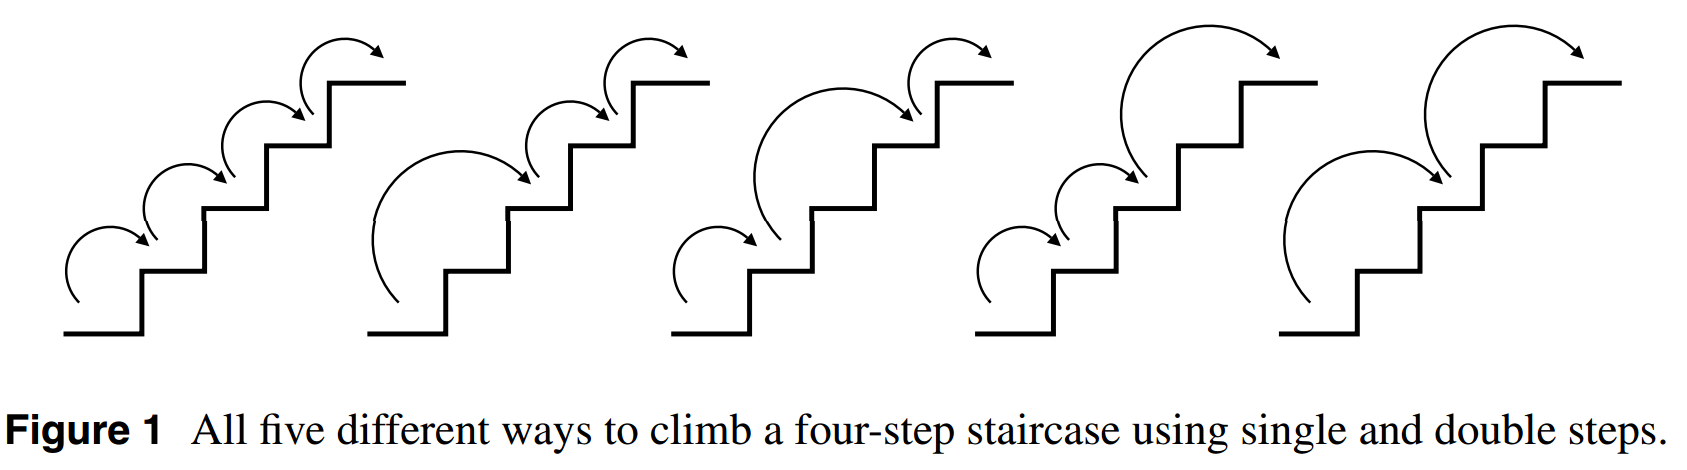
\includegraphics[scale=0.5]{/home/dspataro/git/algorithm_articles/sources/stairs_climbing/images/3stairs}
	\caption{All different ways to climb a 3 stairs staricase using steps of size $1$ or $2$.}
\end{figure}

\end{example}

\begin{example}
	\hfill \\
	Given $n = 4$ the answer is $5$ because there are five ways (See image \ref{fig:stair_example_5} to climb to the top of the stairs:
	\begin{enumerate}
		\item $1$ step + $1$ step + $1$ step + $1$ step
		\item $2$ steps + $1$ step + $1$ step
		\item $1$ step + $1$ step + $2$ steps 
		\item $1$ step + $2$ steps + $1$ step
		\item $2$ steps +  $2$ steps
	\end{enumerate}

\begin{figure}
	\label{fig:stair_example_5}
	\centering
	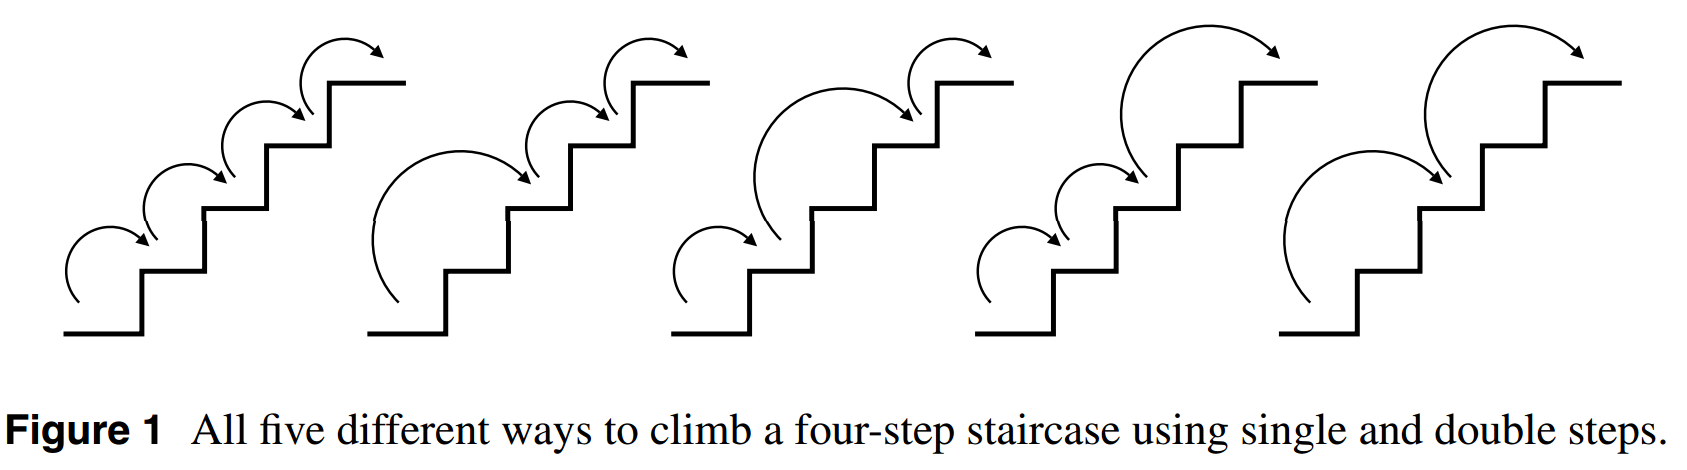
\includegraphics[scale=0.5]{/home/dspataro/git/algorithm_articles/sources/stairs_climbing/images/5stairs}
	\caption{All different ways to climb a four stairs staricase using steps of size $1$ or $2$.}
\end{figure}

\end{example}
	

\section{Clarification Questions}

\begin{QandA}
	\item Can the size of the stair be zero?
	\begin{answered}
		\textit{Yes, the staircase can be made of zero steps.}
	\end{answered}
	
	\item It is guaranteed the answer to fit a built-in integer?
	\begin{answered}
		\textit{Yes, do not worry about overflow.}
	\end{answered}

\end{QandA}

\section{Discussion}
\label{stairs_climbing:sec:discussion}

This is probably one problem that it is easier to tackle by first looking at a few examples so it is easier to see patterns. Table \ref{tab:stairs_climbing_ways_up_tp_7} shows  how many ways there are to climb a stair of lenght $n$ up to $n=7$.

\begin{table}
	\centering
	\begin{tabular}{|c|c|}
		\hline
		$n$ & \textbf{Ways} \\ \hline
		$0$ & $0$ \\ \hline
		$1$ & $1$ \\ \hline
		$2$ & $2$ \\ \hline
		$3$ & $3$ \\ \hline
		$4$ & $5$ \\ \hline
		$5$ & $8$ \\ \hline
		$6$ & $13$ \\ \hline
		$7$ & $21$ \\ \hline
	\end{tabular}
\label{tab:stairs_climbing_ways_up_tp_7}
\caption{All the ways to climb a stair of lenght $n \leq 7$ }
\end{table}

Looking at the table one thing should be immediately noticed i.e. the number of ways to climb the stair of size $n$ is equal to the $n^th$ element of the \textbf{Fibonacci} sequence (starting with two $1$).
Once tht is clear then the solution is straightforward as shown in Listing \ref{list:stairs_climbing_fibonacci}.

\lstinputlisting[language=c++, caption=Solution to the stairs climbining problem with steps of size $1$ and $2$ using Fibonacci.,label=list:stairs_climbing_fibonacci]{/home/dspataro/git/algorithm_articles/sources/stairs_climbing/stairs_climbing_solution1.cpp}

Now, let's have a look at why the seemingly unrelated fibonacci sequence plays a role in this problem. If the problem is looked at as an iterative process in which at each step a certain number of stairs are climbed. For instance if $n = 3$ and:
\begin{itemize}
	\item[-] $1$ step is hopped then the number of remaining steps is $3-1 = 2$. 
	\item[-] $2$ steps are hopped then the number of remaining steps is $3-2 = 1$.
\end{itemize}
When one step is hopped, the problem changes from climbing $n$ stairs to $n-1$ stairs. At this point the problem is seemingly unchanged except for the number of stairs left to climb and the same reasoning can be applied again:
\begin{itemize}
	\item[-] $1$ step is hopped then the number of remaining steps is $(n-1)-1 = n-2$. 
	\item[-] $2$ steps are hopped then the number of remaining steps is $(n-1)-2 = (n-3)$.
\end{itemize}
As can be seen, two decisions are possible i.e. climbing one or two stairs, exactly like in the fibinacci sequence, until either the $n$ step or a point past to it is reached.

\section{Common Variation
}
\subsection{Arbitrary step lengths}
\label{stairs_climbing:sec:arbitrary_steps}
But what happens when the step sizes allowed are not just $1$ or $2$ but an array of $k$ positive values $A=\{s_1 < s_2 < \ldots < s_k\}$. The problem statement for this harder variant of the problem is as follows:

\begin{exercise}
You are climbing a stair case and it takes $n$ steps to reach to the top.

Each time you can either climb $s_1$ or $s_2$ or $\ldots$ or $s_k$ steps where $0 < s_1 < s_2 < \ldots < s_k$. In how many distinct ways can you climb to the top?
\end{exercise}

Note how this problem is equivalent to the easier version described in Section \ref{sec:stairs_climbing_statement_easy} when the allowed step sizes are $s_i = 1$ and $s_2=2$.


%!TEX root = ../main.tex
%%%%%%%%%%%%%%%%%%%%%%%%%%%%%%%%%%
% Links: https://www.geeksforgeeks.org/sort-array-wave-form-2/
%
% Difficulty: Medium Companies: 
%%%%%%%%%%%%%%%%%%%%%%%%%%%%%%%%%%

\chapter{Wave Array}
\label{ch:wave_array}
\section*{Introduction}
We are used to talking about sorting in terms of arranging items in either ascending or descending order. But in general, sorting is the process of arranging items systematically according to a criterion that can be purely arbitrary.

The problem discussed in this lesson is about writing an algorithm for sorting the items of a collection in a rather unusual and peculiar way where the goal is to place elements at even indices such that they all are surrounded by either greater or smaller elements. For instance the collection: $\{1,3,-1,3,2,4\}$ is properly sorted while $\{1,3,-1,1,2,4\}$ is not.

This question has been asked at companies like \textit{Adobe}, and \textit{Google}, mostly during the firsts on-site interview stages as
it is not considered to be a very hard one and you can solve it by writing just a handful of lines.
In fact, provided you come up with the right idea and make no implementation mistakes this problem can be cleared rather quickly. It has, however, proven to be challenging for many, especially in getting it right the first time, and we advise you to spend some time after you have a working draft of the solution to make sure the code is behaving as expected especially on corner cases.






\section{Problem statement}
\begin{exercise}
Given an array $A$ of $n$ integers, arrange the numbers in a wave-like fashion. A valid wave array $X$ has its elements arranged in one of the two following ways:
	\begin{enumerate}
		\item  $x_0 \geq x_1 \leq x_2 \geq x_3 \leq  x_5 \geq \ldots$ where $x_{2i-1} \geq x_{2i} \leq x_{2i+1}$
		\item  $x_1 \leq x_2 \geq x_3 \leq x_4 \geq x_5 \leq \ldots$ where $x_{2i-1} \leq x_{2i} \geq x_{2i+1}$
	\end{enumerate}


	\begin{example}
		\hfill \\
		\label{ex:wave_array:example1}
		Given $A= \{10, 5, 6, 3, 2, 20, 100, 80\}$ the followings are all valid output:
		\begin{itemize}
			\item  \{20, 5, 10, 2, 80, 6, 100, 3\}
			\item  \{10, 5, 6, 2, 20, 3, 100, 80\}
		\end{itemize}
	\end{example}

	\begin{example}
		\hfill \\
		\label{ex:wave_array:example2}
		Given $A= \{20, 10, 8, 6, 4, 2\}$ the followings are all valid output:
		\begin{itemize}
			\item \{20, 8, 10, 4, 6, 2\}
			\item  \{10, 8, 20, 2, 6, 4\}
		\end{itemize}
		
	\end{example}

	\begin{example}
		\hfill \\
		\label{ex:wave_array:example3}
		Given $A= \{10,9,8,7,6,5,4,3,2,1\}$ the following is a output: $\{10, 8, 9, 6, 7, 4, 5, 2, 3, 0,
		1 \}$
		
	\end{example}
\end{exercise}

\begin{figure}
	\centering
	\begin{subfigure}[t]{0.80\textwidth}
		\includegraphics[width=1\linewidth]{/home/dspataro/git/algorithm_articles/sources/wave_array/images/example1.png}
		\caption{Input and solutions for Example \ref{ex:wave_array:example1}.}
		\label{fig:dice_rolls:12faces_dice}
	 \end{subfigure}
	\hfill
	\begin{subfigure}[t]{0.80\textwidth}
		\includegraphics[width=1\linewidth]{/home/dspataro/git/algorithm_articles/sources/wave_array/images/example1.png}
		\caption{Input and solutions for Example \ref{ex:wave_array:example2}.}
		\label{fig:dice_rolls:6faces_dice}
	 \end{subfigure}
	 \hfill
	 \begin{subfigure}[t]{0.80\textwidth}
		 \includegraphics[width=1\linewidth]{/home/dspataro/git/algorithm_articles/sources/wave_array/images/example1.png}
		 \caption{Input and solutions for Example \ref{ex:wave_array:example3}.}
		 \label{fig:dice_rolls:20faces_dice}
	  \end{subfigure}
\end{figure}


\section{Clarification Questions}

\begin{QandA}
	\item Does the array $A$ only contain positive numbers?
	\begin{answered}
		\textit{No, the input numbers can be positive or negative.}
	\end{answered}
	\item Are duplicates in $A$ allowed?
	\begin{answered}
		\textit{Yes, duplicates might be present.}
	\end{answered}
	\item Do the numbers in $A$ lie in a given particular range? If yes which one?
	\begin{answered}
		\textit{No; no assumptions can be made on the values in $A$.}
	\end{answered}
\end{QandA}

\section{Discussion}
\label{wave_array:sec:discussion}
The challenge confronting us is about the creation of an entirely new array $X$ (we, therefore, know from the very beginning we must make a copy of $A$ at some point) that contains the same elements in $A$, arranged in a form that reminds a wave. 
An array of this type has its elements arranged so that they produce a zig-zig-like pattern when plotted on a graph. 

Sequences of numbers of this type can be described as having the property that all of their elements located at even indices are \textbf{all} either 
\textit{local}  \textbf{minima} or  \textbf{maxima}\footnote{An element is a local minimum/maximum if it is lower/higher than its two immediate neighbors.}. 
Identifying a local minimum/maximum is easy but, it is only helpful when we want to test whether a sequence is a valid wave array.

\subsection{Brute-force}
\label{wave_array:sec:bruteforce}
One way to attack this problem is by enumerating every possible arrangement of the elements of $A$ and apply the criteria of wave-array validity discussed above to find a solution. 

We can enumerate all permutations of an array quite easily by using a function like \inline{std::next_permutation](Iterator first, Iterator last)} which 
> Rearranges the elements in the range [first,last) into the next lexicographically greater permutation.

This idea is implemented in Listing \ref{list:wave_array_linear_bruteforce}.

\lstinputlisting[language=c++, caption=Brute-force time solution to the wave array problem.,label=list:wave_array_linear_bruteforce]{/home/dspataro/git/algorithm_articles/sources/wave_array/wave_array_solution3.cpp}


\subsection{Sorting solution}
\label{wave_array:sec:sorting}

As per all array problems, the first question that should come to mind is: \textit{does sorting the elements (we are referring here to a canonical sorting in increasing order) changes the difficulty of the problem?} Incrementally sorted sequences are easy to reason about as they provide strong and clear guarantees on how elements relate to each. Most importantly the same problem is very often a lot easier to solve on a sorted collection than on an unsorted one.
 
If we apply the wave-array validity criterion (discussed above on local minima/maxima) on a sorted array $S=\{s_0 \leq s_1 \leq \ldots \leq s_{n-1}\}$ we notice that $S$ fails the test as there is only one local minimum and local maximum i.e. $s_0$ and $s_{n-1}$ (which also happen to be the global minimum and maximum).

But how $S$ changes if every
element that is located at an even indix is swapped with its subsequent neighbor? When every elements at indices $2i$ and $2i+1$ ($i=0,1,\ldots$) are swapped, then:
$S=\{s_1
\geq s_0 \leq s_3 \geq s_2 \leq s_5 \geq s_4 \leq s_7  \geq \ldots\}$ which is now in better shape to pass the wave-array validity test as now every element at even index is surrounded by smaller (or equal) elements. 

Notice that the elements of $S$ have been shuffled around and that now the element $a_i$ is not located at index $i$ anymore (contrary to how it was originally).
We can see that $a_3$ is now located at index $2$ and it is surrounded by $a_0$ and $a_2$ which are both smaller or equal to $a_3$.
Similarly $a_5$ is now placed at index $4$ and it is surrounded by the elements $a_2$ and $a_4$, both known to be smaller or equal than $a_5$.

We can
use this observation to solve this problem efficiently and elegantly as shown in  Listing \ref{list:wave_array_sorting}.

\lstinputlisting[language=c++, caption=Solution to the wave array problem using sorting.,label=list:wave_array_sorting]{/home/dspataro/git/algorithm_articles/sources/wave_array/wave_array_solution1.cpp}

The code above works by creating a copy of the input array $A$ named $B$, which is subsequently sorted. The code then proceeds in swapping every element located at an even location with the element after it. You can see the \inline{swap} operation is applied to the iterators \inline{it} and \inline{it+1} and that at the end of each iteration \inline{it} is incremented by $2$. This, together with the fact \inline{it} initially pointer to the first even element  at location $0$, effectively means that only pairs of items at indices of the form $(2i, 2i+1)$ are swapped.

The code above is considered good  as its time and space complexity are $O(nlog(n))$
and $O(n)$, respectively.

In some cases, the interviewer might ask you to return, among all possible valid arrangments, the one being the lexicographically minimum. If it is the case the solution proposed below won't
work and it should not be attempted.


\subsection{Linear time solution}

Despite the solution using sorting presented in Section \ref{wave_array:sec:sorting} is already good enough to
possibly clear the interview, there exists a solution that works in linear time and that is as easy to
implement and explain. The core idea is always the same: elements at even index should always be
greater (or smaller, equivalently) than their adjacents neighbors. Only this time we will enforce it in a single pass on the array, by
swapping elements at even indices with their direct neighbors (to the left and to the right) if they happen to be smaller in such a way that the largest element among  $x_{2i-1},x_{2i},x_{2i+1}$ always end up going to the location $2i$.

We can do that by iterating over all even indices and performing the following operations:
\begin{enumerate}
	\item if the current element $a_{2i}$ is smaller than the element $a_{2i-1}$ then swap them. 
	\item if the current element $a_{2i}$ (possibly newly assigned from the previous step) is smaller than the element $a_{2i+1}$ then swap them.
\end{enumerate}

At this point we have effectively placed the largest among $x_{2i-1},x_{2i},x_{2i+1}$ at the location $2i$ and we can proceed to the next even element $a_{2(i+1)}$. 

See Listing \ref{list:wave_array_linear} for a possible implementation of this idea.

\lstinputlisting[language=c++, caption=Linear time solution to the wave array problem.,label=list:wave_array_linear]{/home/dspataro/git/algorithm_articles/sources/wave_array/wave_array_solution2.cpp}

Notice that the code above performs some checks on the corner elements so that we do not perform out-of-bound accesses.

\textbf{This solution is optimal as it runs in $o(n)$ space and time.} 

Like the solution using sorting, it does not work when the lexicographical minimum arrangement should be returned.



%!TEX root = ../main.tex
%%%%%%%%%%%%%%%%%%%%%%%%%%%%%%%%%%
% Links:
%
% Difficulty: Companies: 
%%%%%%%%%%%%%%%%%%%%%%%%%%%%%%%%%%

\chapter{First positive missing}
\label{ch:first_positive_missing}
\section*{Introduction}

This chapter addresses a fairly common problem posed during on-site interviews for which there are a number of solutions which vary widely in terms of time and space complexity.

Finding what most interviewers would consider the \quotes{best} solution in terms of asymptotic complexity can be challenging therefore in needs a more in depth analysis than some other problems posed in this book.

It is common for interviewers to pose this problem using a short and purposely vague statement.
It is, therefore,  important to ask questions to ensure all aspects of the problem are well understood before attemping a solution.  \footnote{ We think a good way of doing this is to repeat out loud a summary of your understanding of the problem to the interviewer.}

\section{Problem statement}
\begin{exercise}
	Write a function that, given an unsorted integer array $A$, returns the smallest positive integer not contained in $A$.

	\begin{example}
		\hfill \\
		Given $A=\{ 1, 0, -1, -2\}$ the answer is $2$.
	\end{example}
	
	\begin{example}
		\hfill \\
		Given $A=\{ 2, 3, -7, 6, 8, 1, -10, 15\}$ the answer is $4$.
	\end{example}
	
	\begin{example}
		\hfill \\
		Given $A=\{ 1, 0, -1, -2\}$ the answer is $2$.
	\end{example}
\end{exercise}
	
\section{Clarification Questions}

\begin{QandA}
	\item \begin{questionitem} \begin{question} Are the input numbers always positive?  \end{question} 	 
    \begin{answered}
		\textit{No, the array contains positive and negative numbers.}
	\end{answered} \end{questionitem}

	\item \begin{questionitem} \begin{question} Are all the elements distinct?  \end{question} 	 
    \begin{answered}
		\textit{No, the array might contains duplicates.}
	\end{answered} \end{questionitem}
	
	\item \begin{questionitem} \begin{question} Can the input array be modified?  \end{question} 	 
    \begin{answered}
		\textit{Yes.}
	\end{answered} \end{questionitem}

	\item \begin{questionitem} \begin{question} Can the size of the array be zero? In other words, can the array be empty?  \end{question} 	 
    \begin{answered}
		\textit{No, the input array contains at least one element.}
	\end{answered} \end{questionitem}

	\item \begin{questionitem} \begin{question} Is $0$ a valid output?  \end{question} 	 
    \begin{answered}
		\textit{No, only strictly positive numbers should be returned.}
	\end{answered} \end{questionitem}

\end{QandA}

\section{Discussion}
\label{first_positive_missing:sec:discussion}
This problem has a solid real-life application.
Consider how an OS might assign PID\footnote{A number used (in UNIX part of the process control block) to uniquely identify a process within the OS. In Unix, process IDs are usually allocated on a sequential basis, beginning at 0 and rising to a maximum value (usually 65535) which varies from system to system. Once this limit is reached, allocation restarts at zero and again increases. However, for this and subsequent passes any PIDs still assigned to processes are skipped.}s to processes. One approach would be to keep a list of all the PIDs for all the processes running, and once a new one is fired up, the OS will assign it the smallest PID \textbf{not already assigned} to any other process. 

In a highly dynamic environment like the OS with thousands of applications active at the same time; the focus of the solution should be speed as you want the process to be up and running as quickly as possible. 


\subsection{Brute-force}
One of the simplest approaches is to simply search $A$ for the missing number incrementally,  starting from $1$. 
The practical reality of this approach is that we have to perform a search operation in $A$ for each number from $1$ onward \textbf{until the search fails}.
This algorithm is always guaranteed to return the smallest missing number given that we perform the searches in order, with the smallest numbers being searched first. 

Listing \ref{list:first_positive_missing_bruteforce} shows an implementation of this using \inline{std::find()} as a means to do the actual search in the $A$. 
 
\lstinputlisting[language=c++, caption=Two bruteforce solution implementations the problem of finding the smallest missing positive integer in an array.,label=list:first_positive_missing_bruteforce]{sources/first_positive_missing/first_positive_missing_solution4.cpp}

This is often considered a poor solution (as a rule of thumb, in the context of coding interviews, brute-force solutions always are) as it has a
complexity of $O(n^2)$ time and $O(1)$ space.

It does, however, have some advantage in being  easy and fast to write, and avoiding implementations mistakes due to simple logic and small amount of code involved.


\subsection{Sorting}
\label{first_positive_missing:sec:sorting}

The second most intuitive approach (after brute-force)is sorting the input as having the numbers sorted is helpful for easily coming up with a faster solution.

When the $A$ is sorted, we know the positive numbers in it will all be appearing \textbf{in an ordered fashion} from a certain index $k\geq 0$ onwards (the positions from index $0$ to $k-1$ are occupied by negatives or zeros). 

We also know that, if no number is missing in $A[k \ldots n-1]$, then we would expect to see: 
\begin{itemize}
	\item $A[k]=1$
	\item $A[k+1]=2$
	\item $A[k+2]=3$
	\item $\ldots$
	\item $A[n-1]=n-k+1$
\end{itemize}

i.e. all numbers from $1$ onward appear in their natural order $(1,2,3, \ldots (n-k+1))$ from the cell at index $k$ to the end of $A$. 
If any of these numbers are missing then we would not be able to see such a sequence.

The goal of this problem is to find the first number that is missing from that sequence.  We can do that by finding the first element among $A[k \ldots n-1]$  where the condition $A[k+i]=i+1$ with $(i=0,1,2, \ldots)$ is \textbf{false}. When this happens, we can conclude the missing number is $i+1$.
If such a cell does not exist (every cell satisfies the condition above), then we know that the missing number is $A[n-1]+1$.

For example, consider the array $A=\{ 9,-7,0,4,5,2,0,1\}$. When sorted, the array
becomes $A=\{ -7,0,0,1,2,4,5,9\}$. The positives start at index $k=3$:
\begin{itemize}
	\item $A[3+0] = 1$ (test passes)
	\item $A[3+1] = 2$ (test passes)
	\item $A[3+2] = 4$ (\textbf{test fails})
\end{itemize}
As we can see, the test fails after three tries and therefore we can conclude the missing number is $3$.


Now let's consider the array $B=\{ 3,-7,0,4,5,2,0,1\}$ which is exactly the same as in the previous example, with the exception that we have swapped a $9$ for a $3$. When sorted, the array
becomes $B=\{ -7,0,0,1,2,3,4,5\}$ which contains no gaps between any of the positive numbers. As before, the positives start at index $k=3$ but this time every element passes the test:
\begin{itemize}
	\item $A[3+0] = 1$ (test passes)
	\item $A[4+1] = 2$ (test passes)
	\item $A[4+2] = 3$ (test passes)
	\item $A[4+3] = 4$ (test passes)
	\item $A[4+4] = 5$ (test passes)
\end{itemize}
We can clearly see that the missing number is $6 = A[8]+1 = A[n-1]+1$.

An implementation of this idea is shown in Listing
\ref{list:first_positive_missing_sorting}.

\lstinputlisting[language=c++, caption=Solution to the problem of finding the smallest missing positive integer in an array.,label=list:first_positive_missing_sorting]{sources/first_positive_missing/first_positive_missing_solution1.cpp}

Note that:
\begin{itemize}
	\item the iterator \inline{it} always points at the currently evaluated element. 
	It is initialized to either:
	\begin{itemize}
		\item the \textbf{smallest positive} in the sorted array;
		\item to one element past the end of the array if no positives are present.
	\end{itemize}
	\inline{it} is moved to its initial location by using the \inline{std::find_if} function from the STL which runs in linear time. We might have used binary search to perform this task, but that would not have signficantly helped in  lowering the overall asymptotic time complexity as the sorting operation itself costs $O(nlog(n))$ and the subsequent \inline{while} loop runs in linear time. 
	\item \inline{expected} is a variable holding the value that is expected to be found where \inline{it} is pointing to (the value $i+1$ mentioned above).
	\item if the \inline{while} runs to completion because we have examined every element of $A$ (\inline{it ==std::end(A)}) then \inline{expected} points to \inline{A.front()+1}.
	\item if no positives are present, then the \inline{while} does not even run once and $1$ is returned.
\end{itemize}

This is considered a good solution with an overall time and space complexity of $O(nlog(n))$ and $O(n)$ respectively. It is, however, not optimal, solutions with better time and space complexities exist.  


\subsection{Linear time and space solution}
\label{first_positive_missing:sec:linear_space}

Examining the problem more closely  we immediately notice that the missing number will always be
in the range $[1,n]$, where $n$ is the size of the input array. \textbf{Why is this the case?}
We can draw this conclusion by considering which input can possibly lead to the largest possible output: among
all possible arrays of size $n$, only one configuration leads to the highest missing number: $A =
\{1,2,3,4, \ldots ,n\}$ i.e. the configuration where all numbers from $1$ to $n$ are present. All the other configurations contain duplicates,
negative or numbers higher than $n$ which forces the input to have ``holes'' (i.e. missing numbers in the range $[1,n]$). 

This fact can be exploited to keep track of which positive numbers from
$1$ to $n$ are present in $A$. We can use an array of booleans flags of size $n$ to store this information. Therefore, all we have to do is set the $x^{th}$ flag to true for each number  $x$ in $A$ in the range $[1,n]$.
Eventually, this array of flags contains the answer, which can be found by scanning through it linearly to find the first \textbf{false} element which signals that this is the first missing element.

An implementation of the idea above is found in Listing \ref{list:first_positive_missing_constant_space}.

\lstinputlisting[language=c++, caption=Solution to the problem of finding the smallest missing positive integer in an array.,label=list:first_positive_missing_constant_space]{sources/first_positive_missing/first_positive_missing_solution2.cpp}


The code in Listing \ref{list:first_positive_missing_linear_space} works in two phases:
\begin{enumerate}
	\item For each number \inline{x} of $A$ in the range $[1,n]$, we remember we have found it by marking the cell at index \inline{x-1} in \inline{F}.
	\item We find if exists the first cell in \inline{F} containing false which means the corresponding element was not found in $A$. If a false cell does not exist then we can conclude the missing number is $n+1$.
\end{enumerate}
This approach is considered good and it has time and space complexity both equal to $O(n)$.

As an alternative, instead of an array, we can use a hashmap to keep track of which element has
already been seen as the array is scanned from left to right. This might have advantages in some cases, especially when $n$ is large but there are many duplicates in $A$. 


\subsection{Linear time and constant space solution}
\label{first_positive_missing:sec:constant_space}

As mentioned above, the optimal solution does not use any additional space but shares the idea of keeping track of which
element has been found with the solution described in Section \ref{first_positive_missing:sec:linear_space}. 

In order to avoid using additional space we have to somehow implement the functionality the array \inline{F} (in the code above) provides using the input array itself. Doing so sounds harder than it is, especially before we realize that we can store the information about a positive number being pres

The previous solutions have already demonstrated that we can safely ignore every negative number in $A$, and that the largest output we can ever hope to get is always less than the number of positives in $A$. For instance, if we have an array of size $n$ with $x$ negatives and $y$ positives ($n=x+y$), then the largest possible output we can get is: $y+1$. 

As an example, let's consider the array $A=\{-1, -2, -3, 0, 1, 2, 3\}$ which has $x=4$ negatives and $y=3$ positives ($n=7$). We can see that the missing number is $4=y+1$ and also that, if we substitute any positive (or negative or zeros for that matter) number with a different positive, the output of the function will \textbf{not increase}. 

The idea is to loop through $A$ and, for each number $x>0$ , store the information about $x$ being present in $A$ in some cell of $A$ itself. But which one? What we want is to have a mapping from the positives in $A$ to indices of $A$. We can use this mapping to choose the cell in which we remember whether a number is present or not by changing its sign.

Noe that, if $A$ contains $y$ positive, then we have $y$ cells to which we can change the sign from positive to negative. In our quest to create this 1-to-1 mapping one problem, the problem we face is that $A$ is unsorted and positives and negatives are all shuffled together. Therefore, the first step would be to rearrange the elements so that all the positives appear before all the negatives. In this way creating the mapping becomes much easier. If all $y$ positive are located from index $0$ to $y-1$, then every time we process an element of $x$ of $A$, which value is between $1$ and $y$ ($1 \leq x \leq y$), we can change the value of the cell at index $x$ to remember the fact the value $x$ is present in $A$. The remaining problem at this point is to rearrange $A$ so that all positives appear before all negatives and zeros in an efficient manner.


Given an unsorted array, we can rearrange its elements so that all positives are before all negatives by using a two-pointer technique where we use  - unsurprisingly -  two pointers $s$ and $e$ pointing initially to index $0$ and $n-1$, respectively.
The idea is to keep moving $s$ towards the end of the array and $e$ towards the start, until $s$ points to a positive and $e$ points to a negative. At this point, $s$ points to a value that should appear after the element pointed by $e$ and therefore we can swap those values. 
If we keep repeating this process until $s>=e$, eventually all the pairs of misplaced elements (a negative appearing before a positive) are swapped and the final array is arranged so that all negatives appear in the first $x$ positions of the array.

Consider for instance the array $A=\{-1, 1, 2,-2 0,3,-3\}$. Initially $s=0$ and $e=6$. We first move $s$ to the first positive which happens to appear at index $1$. Similarly, we move $e$ to the left towards the first negative which appears at index $6$. The elements pointed by $s$ and $e$ are swapped, and $A=\{-1, -3, 2,-2 0,3,1\}$.

The same process is repeated and after they are moved, $s=2$ and $e=4$. 
The values they point to are swapped leaving $A=\{-1, -3, 0,-2 2,3,1\}$. When the pointers are next moved, they would cross, and this signals the rearrangement is finally complete. It is important to note that the aim of this process is not to sort the array, but to simply make all the negatives appear before all the positives (therefore still allowing the positives and the negatives to appear in any order).


Once all the numbers in $A$ are processed this way, similar to what we did in step $2$ of the solution running in linear time and space (where we used the array `F`), we can scan the portion of $A$ from index $0$ to $y$ looking for positives. 
If we find one at index $k$, it means that the element $k+1$ is missing from the array as, if it was present,  it would have undergone a sign change. 
If all those cells contain negative, then it means that the missing number is $n+1$.

This idea is implemented in Listing \ref{list:first_positive_missing_linear_space} shown below.

\lstinputlisting[language=c++, caption=Linear time and constantspace solution to the problem of finding the smallest missing positive integer in an array.,label=list:first_positive_missing_linear_space]{sources/first_positive_missing/first_positive_missing_solution3.cpp}

The two phases of this solution are packaged into two functions:
\begin{itemize}
	\item \inline{first_positive_missing_constant_space} builds on it and uses the rearrangement to mark the presence of any element $x$ in the range $[1,y]$ by changing the sign of the cell at index $x-1$. When it is done with it, it proceeds in finding the answer by searching for the smallest index in $i$ containing a positive.
	\item \inline{divide_pos_neg} is responsible for rearranging the input array as discussed above
\end{itemize}

The complexity of this approach is linear in time and constant in space which is optimal.
%!TEX root = ../main.tex
%%%%%%%%%%%%%%%%%%%%%%%%%%%%%%%%%%
% Links: https://www.toptal.com/algorithms/interview-questions
%
% Difficulty: 
% Companies: 
%%%%%%%%%%%%%%%%%%%%%%%%%%%%%%%%%%

\chapter{Exponentiation}
\label{ch:exponentiation}
\section*{Introduction}
This chapter addresses a common problem, that ask us to implement a function in order to calculate the power of an integer.  
It is fairly easy to come up with a good solution that works in linear time and that, 
when implemented properly, can already be enough to get the green light from the interviewer and pass the interview stage.
However, in order to be sure to ace the question, we need to push ourselves a bit further than this and develop a more sophisticated and efficient solution.
In order to achieve this goal, we will use an old and well-refined idea: the *exponentiation by squaring*, which can be
applied not only to integers but also to many other mathematical objects, such as polynomials or
matrices (for instance, it can be used to calculate the $k^{th}$ Fibonacci number in $log_2(k)$ steps), and that will be key to the solutions we present here. 

\section{Problem statement}

\begin{exercise}
Implement a function that given two positive integers $n$ and $k$ calculates $n^k$.

    \begin{example}
        \hfill \\
        Given $n=2$ and $k=3$ the function returns $8$.
    \end{example}

    \begin{example}
        \hfill \\
        Given $n=5$ and $k=2$ the function returns $25$.
    \end{example}

\end{exercise}

\section{Clarification Questions}

\begin{QandA}
    \item \begin{questionitem} \begin{question} Should the function handle the case where $k=0$?  \end{question}      
    \begin{answered}
        \textit{Yes $k=0$ is a valid input.}
    \end{answered} \end{questionitem}
    
    \item \begin{questionitem} \begin{question} Should the function handles integer overflow?  \end{question}      
    \begin{answered}
        \textit{No overflow should not be accounted for. }\footnote{
            This clarification question can however, lead to a follow-up discussion on how such scenario can be handled and it can very well go in the many directions: 
            \begin{itemize}
                \item how to represent and manipulate infinite precision numbers,
                \item examples of production libraries providing infinite precision, etc. (the \href{https://gmplib.org/}{GMP library}\cite{cit::web::gmplibrary} probably being the most known).
                \item how overflow errors can be handled? (Exceptions, error codes, \href{https://en.cppreference.com/w/cpp/language/ub}{UB}\cite{cit::std::ub}?)
            \end{itemize}
            }
    \end{answered} \end{questionitem}
        
\end{QandA}

\section{Discussion}
\label{exponentiation:sec:discussion}

Exponentiation is such a basic operation: we all know how to calculate powers by means of performing a number of consecutive multiplications. 
This method stems  directly from the definition of exponentiation, which involves two numbers $n$ (the base) and $k$ (the exponent) and it is usually written as $n^k$ (pronounced as *"$n$ raised to the power of $k$"* or *the ${k^{th}}$ power of $n$"*):
$n^k = n \times n \times n \ldots  \times n$ where we multiply the base exactly $k$ times with itself
to obtain the result. 

This simple algorithm embedded in the definition can be coded in just a few lines and a possible iterative implementation is shown in Listing
\ref{list:exponentiation_linear}.


\lstinputlisting[language=c++, caption=Iterative linear time solution.,label=list:exponentiation_linear]{sources/exponentiation/exponentiation_solution1.cpp}

The code calculates the answer, stored in the variable \inline{ans}, by multiplying \inline{ans} itself and \inline{n}, \inline{k} times like we would do with on a blackboard and exactly like stated in the definition of exponentiation above.
Notice that:
\begin{itemize}
    \item Listing \ref{list:exponentiation_linear} assumes $k >=0$,
    \item when $k=0$ the while loop is not executed at all and the final result is $1$ (which is correct as the result of raising any positive to the power of $0$ is $1$.)
    \item the time complexity is $O(k)$ as the while loop decreases the value of $k$ by $1$ at each iteration;
    \item the space complexity is constant. 
\end{itemize}

\subsection{Using recursion}
When discussing this solution, the interviewer might explicitly ask for a recursive solution. The definition of power by repetitive multiplication already provides all the ingredients to write one, and in particular, it should be noticed that we can regroup the operations in the definition above so that: $n^k = n \times n^{k-1}$ which shows that the ${k^{th}}$ power of $n$ is function of its ${(k-1)^{th}}$ power. 

Listing \ref{list:exponentiation_linear_recursive}  shows a recursive code implementing this idea.

\lstinputlisting[language=c++, caption=Recursive linear solution.,label=list:exponentiation_linear_recursive]{sources/exponentiation/exponentiation_solution5.cpp}

Listing \ref{list:exponentiation_linear_recursive} runs in $O(k)$ time and space as:
\begin{itemize}
    \item the base case $k=0$ is reached only after $k$ steps as each recursive call decreases the value of $k$ by $1$ and each call costs constant time; 
    \item we need to use space for the activation record of each of the $O(k)$ recursive calls.
\end{itemize}



\subsection{Binary fast exponentiation}
\label{exponentiation:sec:fast_exponentiation}
The recursive solution showed above was built on the notion that the ${k^{th}}$ power of $n$ is function of its ${k-1^{th}}$ power. We have obtained this result by simply regrouping the definition of exponentiation given in the introduction of this chapter. However, this is not the only possible way of regrouping these multiplications as, for instance, we can calculate $n^k$ as $n^{4} \times n^{k-4}$.
This is possible thanks to the following two well-known properties of powers:

\begin{enumerate}
    \item if $x+y=k$ then, $n^k = n^x  n^y = n^{x+y}$ 
    \item if $x \times y=k$ then, $n^k = (n^x)^y$
\end{enumerate}

How can we use this to speed up the exponentiation process? For instance, let's consider what happens when  $k$ is a power of $2$.
All it takes to calculate $n^k$ is knowing the value of $n^{\frac{k}{2}}$, and in turn, all it takes to calculate $n^{\frac{k}{2}}$ is $n^{\frac{\frac{k}{2}}{2}}$ and so on, $\ldots$ You see where this reasoning is heading towards.
Eventually the exponent would be one, and at that point we know the answer right away.

Because at every step the exponent is divided by $2$, after $log_2(k)$ steps we have all the ingredients to calculate the answer as $n^k : n^{\frac{k}{2}} \times n^{\frac{k}{2}} = (n^{\frac{k}{4}} \times n^{\frac{k}{4}}) \times (n^{\frac{k}{4}} \times n^{\frac{k}{4}}) = \big ( (n^{\frac{k}{8}} \times n^{\frac{k}{8}}) \times (n^{\frac{k}{8}} \times n^{\frac{k}{8}}) \big ) \times \big ( (n^{\frac{k}{8}} \times n^{\frac{k}{8}}) \times (n^{\frac{k}{8}} \times n^{\frac{k}{8}}) \big )  = \ldots$


We have effectively reduced the time complexity down to $log_2(k)$ \textbf{when $k$ is a power of two}.
But what about the general case? Notice that we can split $k$ in half every time $k$ is even (and that when $k$ is a power of $2$ all the intermediate division lead to an even number), and therefore we can start by applying the idea above only when $k$ is even and relying on the ($1$,$k-1$) split in all the other cases. 


In other words, the idea is to calculate the answer by multiplying two smaller powers: $n^p$ and $n^q$ with $p,q < k$. The value of $p$ and $q$ depends on the parity of $k$ (whether $k$ is even or odd) and more in particular we want:
  \[
    n^k = \begin{cases}
                p=q \Longrightarrow n^{\frac{k}{2}} \times n^{\frac{k}{2}}, & \text{if  k even}\\
                p=1, q=k-1 \Longrightarrow n \times n^{k-1}, & \text{if k odd}\\
            \end{cases}
  \]
This allows for the number of multiplication to be reduced by half all the times that $k$ is even but also crucially, when $k$ is odd as $n^{k-1}$ can be calculated by reducing the number of multiplications by half because $k-1$ is even.

Clearly, this approach is inherently recursive and
can be coded as such easily as shown in Listing \ref{list:exponentiation_fast}.

\lstinputlisting[language=c++, caption=Recursive $O(log_2$ solution to the exponentiation problem.,label=list:exponentiation_fast]{sources/exponentiation/exponentiation_solution2.cpp}

The code works similarly to how the linear time recursive solution works except for the special treatment $k$ receives when it is even. 

This solution has a time complexity of $log_2(k)$. The intuitive idea is that in the worst-case scenario, for every two invocations of the \inline{exponentiation_fast} function we split the value of $k$ in half anyways.

\subsection{Iterative solution using bit manipulation}

Another way to tackle this problem is by looking at the binary representation of the exponent $k =
b_0 \times 2^0 + b_1 \times 2^1 + \ldots + b_l \times 2^l$ where $b_i$ as a binary digit.
When plugging $k$ into the formula for the calculation of $n^k$, the following is obtained (and by applying the properties of powers shown above):
\[
    \begin{array}{lcl}
        n^k & = &  n^{b_0 \times 2^0 + b_1 \times 2^1 + \ldots + b_l \times 2^l} \\
        & = & n^{b_0 \times 2^0} \times n^{b_1 \times 2^1} \times \ldots \times n^{b_l \times 2^l} \\
        & = & (n^{2^0})^{b_0} \times  (n^{2^1})^{b_1} \times \ldots \times (n^{2^l})^{b_l} \\
        & = & (n^{2^0})^{b_0} \times  (n^{2^1})^{b_1} \times \ldots \times (n^{2^l})^{b_l} 
    \end{array}
\]

It is clear that the term $i^{th}$ in the final multiplication chain contributes to the final result only when the corresponding value of $b_i$ is set to $1$, because if it is $0$ then the term contribution is $1$ (which is the neutral element for multiplication).
Additionally, as $i$ increases, $n$ gets squared at each step, as $i$ is in the formula an exponent for $2$. 


The idea above can be used to implement
a fast exponentiation iterative solution by looking only at the bits of $k$, and using the formula above to calculate the answers accordingly.
Listing \ref{list:exponentiation_fast_iterative} and \ref{list:exponentiation_fast_iterative_alternative} shows two  possible ways of doing this.

\lstinputlisting[language=c++, caption=Logaritmic solution based on the analysis of the bits of the exponent.,label=list:exponentiation_fast_iterative]{sources/exponentiation/exponentiation_solution3.cpp}


The code in Listing \ref{list:exponentiation_fast_iterative}  works by keeping track of two quantities:
\begin{enumerate}
    \item \inline{ans}: a variable holding the partial calculations of the answers along the multiplication chain and, 
    \item \inline{n} which stores the value of $n$ raised to $2$ to the power of the current iteration index $i$. The value of $n$ is squared at each iteration.
\end{enumerate}
The loop is used to inspect the $i^{th}$ bit of $k$ and when it is set, \inline{ans} is multiplied with the current value hold by \inline{n}. 


The complexity of this approach is $O(log_2(k))$, because the algorithm does not perform more iteration than the number of bits of the exponent $k$.
Thus, at most $\lfloor log(k) \rfloor$ squarings and multiplications are performed.
If native types like \inline{unsigned} are used, then the complexity is constant as these types have a finite precision and therefore a fixed number of bits (the same reasoning holds for all the solutions discussed in all the sections above). 

Listing \ref{list:exponentiation_fast_iterative_alternative} shows an alternative implementation which is slightly more sophisticated and efficient as it stops as soon as it notices there is no bit set in $k$ anymore (when $k$ is zero),  while Listing \ref{list:exponentiation_fast_iterative} iterates blindly over all the bits of $k$.
In practice, this might not be a real or even measurable advantage.

\lstinputlisting[language=c++, caption=Alternative implementation of Listing \ref{list:exponentiation_fast_iterative}.,label=list:exponentiation_fast_iterative_alternative]{sources/exponentiation/exponentiation_solution4.cpp}

Finally, we should note that, because one of the constraints of the problem is that overflow is guaranteed to never occur, then we are assured that $k$ is a relatively small number and we can safely assume it is smaller than $64$, otherwise we would need data types with a capacity of more than $64$ bits to store the answer.
Under this constraint, the logarithmic time solution might also not provide a measurable speed-up or it might even be slower, due to the fact that the linear time solution features a simple loop with basic operations that can be well optimized by the compiler optimizer.


In the introduction, we also mentioned that exponentiation not only applies to numbers but that can be basically applied to a larger class of objects, matrices for instance. The codes developed during the discussion of this problem can be easily extended so that they work on any type providing the \inline{operator*()},\inline{operator>>()} and the
\inline{operator\&()} operators by using \inline{template}s.


\section{Common Variations}

\subsection{Fibonacci numbers - Problem statement }

\begin{exercise}
Write a function that given an integer $n$ returns the $n^{th}$ Fibonacci number. 
Your solution should run in $O(log(n))$ time. 

    \begin{example}
        \hfill \\
        Given $n=44$ the function returns $701408733$
    \end{example}

\end{exercise}


%!TEX root = ../main.tex
%%%%%%%%%%%%%%%%%%%%%%%%%%%%%%%%%%
% Links:
% https://medium.com/@rsinghal757/kadanes-algorithm-dynamic-programming-how-and-why-does-it-work-3fd8849ed73d
% https://en.wikipedia.org/wiki/Maximum_subarray_problem
% https://www.geeksforgeeks.org/maximum-subarray-sum-using-divide-and-conquer-algorithm/
% https://www.geeksforgeeks.org/largest-sum-contiguous-subarray/ Difficulty: Medium Companies:
% Facebook paypal yahoo microsoft linkedin mazaon 
%%%%%%%%%%%%%%%%%%%%%%%%%%%%%%%%%%

\chapter{Largest sum in contiguous subarray}
\label{ch:max_sum_continguous_subarray}
\section*{Introduction}
When it comes to coding interviews, dynamic programming questions are among the most feared and challenging:
one of the most famous and iconic of this category is the  \textit{Largest sum in contiguous subarray} problem. This is not only a still frequently asked question, but it also has many real-life applications in science including, but not limited to, genomic sequence analysis (to identify certain protein sequences) and computer vision (to identify the brightest or darkest part of an
image). 


In this chapter, we will investigate how to efficiently solve this problem and its most popular variations, starting from the inefficient brute-force solution, which will serve as a starting point for our journey towards efficiency. This solution will then be improved by using the concept of avoiding duplicate calculation which is central to DP\cite{bellman1954} (see Section \ref{sect:appendix:DP}). 
Finally, we will study and develop an intuitive idea of what is considered to be the reference algorithm for this problem which allows us to solve this problem efficiently and elegantly.

\section{Problem statement}
\begin{exercise}
Write a function that finds the largest sum of a contiguous sub-array (containing at least one element) within an array $A$
of length $n$.

Formally, the task is to find two indices $ 0 \leq i \leq j < n$ s.t. the following sum is maximized:
\[
\sum_{x=i}^j   = A[x] = A[i] + A[i+1] + \ldots + A[j] 
\]

	\begin{example}
		\hfill \\
		Given $A=\{-2, -5, \underbrace{6, -2, -3, 1, 5}\text{}, -6\}$ then the answer is $7$ which can
		be obtained by summing all elements from index $2$ to $6$ i.e. $\sum_{i=2}^7 A[i] = 7$
	\end{example}

	\begin{example}
		\hfill \\
		Given $A=\{-2, 1, -3, \underbrace{4, -1, 2, 1}\text{}, -5, 4\}$ then the answer is $6$ which can
		be obtained by summing all elements from index $3$ to $6$ i.e. $\sum_{i=3}^6 A[i] = 6$
		
	\end{example}
\end{exercise}

\section{Clarification Questions}

\begin{QandA}
	\item \begin{questionitem} \begin{question} Are the elements all positive or negative?  \end{question} 	 
    \begin{answered}
		\textit{No, the input numbers can be either positive, or negative.}
	\end{answered} \end{questionitem}
	
	\item \begin{questionitem} \begin{question} Is the array sorted?  \end{question} 	 
    \begin{answered}
		\textit{No, the array is not sorted.}
	\end{answered} \end{questionitem}

	\item \begin{questionitem} \begin{question} Is is guaranteed the final result fits an \inline{int}?  \end{question} 	 
    \begin{answered}
		\textit{Yes, you should not worry about interger overflow.}
	\end{answered} \end{questionitem}
	
\end{QandA}

\section{Discussion}
\label{max_sum_continguous_subarray:sec:discussion}
A couple of important observations can be made after reading the problem statement:
\begin{itemize}
	\item If the array only contains non-negative numbers, then the problem becomes trivial, because the answer is the sum of the whole array;
	\item If, on the contrary, the array contains only  numbers lower than or equal to zero, then the answer coincides with the largest number in $A$ (if the constraint on the non-empty size of the sub-array is relaxed, then the answer in this case is always zero.);
	\item  The answer is unique, but more than one sub-array might sum up to that value.
\end{itemize}

\subsection{Brute-force}
\label{sec:max_sum_continguous_subarray_bruteforce}
One way to tackle this problem is to look at the sum of all possible sub-arrays and return the largest.
The idea is that, for all elements $A[i]$, the sum of \textbf{all} sub-arrays having it as starting element can be calculated as shown in Listing
\ref{list:max_sum_continguous_subarray_bruteforce}.

\lstinputlisting[language=c++, caption=Cubic time brute-force solution,label=list:max_sum_continguous_subarray_bruteforce]{sources/max_sum_continguous_subarray/max_sum_continguous_subarray_solution1.cpp}


The code in Listing \ref{list:max_sum_continguous_subarray_bruteforce} enumerates all possible pairs of indices $i < j$, and for each of them it calculates the sum of the elements of $A$ between $i$ and $j$. Among all of those sums, the largest is returned. 

This approach is correct but it is unnecessarily slow, and it has a time complexity of $O(n^3)$: there are $O(n^2)$ ordered pairs $(i,j)$ each identifying a sub-array, and calculating the sum of a single sub-array costs $O(n)$ (the call to \inline{std::accumulate}), for a grand total of $O(n^3)$. 
This is considered a poor solution: it is quite far off from the optimal linear time complexity solution that exists for this problem.



\subsection{Improving the Brute-force}
\label{max_sum_continguous_subarray:sec:bruteforce_improved}
We can improve the brute-force solution proposed in the Section \ref{sec:max_sum_continguous_subarray_bruteforce} above if we explicitly avoid calculating the sum of a sub-array over and over again.
Given two indices $i$ and $j$ the corresponding sub-array sum can be obtained in constant time by using a pre-calculated prefix sum (see Section \ref{sect:appendix:prefix_sum}) of the input array.
This allows for constant-time computation of the sum of any sub-array in $A$. Given an array $Y$ containing the prefix sum for the
array $A$ then the sub-array sum between indices $i$ and $j$ is equal to: $Y[j]-Y[i-1]$ where $Y[-1] = 0$.

The code below shows how this idea can be used to bring the time complexity of the brute-force solution above down to $O(n^2)$. 

Notice how the call to \inline{std::accumulate} is substituted with a simple $O(1)$ operation on the prefix sum that is pre-calculated using the function \inline{prefix_sum} (which crucially runs in linear time).


\lstinputlisting[language=c++, caption=Brute-force quadratic time and linear space solution using prefix-sum.,label=list:max_sum_continguous_subarray_bruteforce_improved]{sources/max_sum_continguous_subarray/max_sum_continguous_subarray_solution3.cpp}

Despite the dramatic improvement in time complexity obtained with this new solution, the code in Listing
\ref{list:max_sum_continguous_subarray_bruteforce_improved} is still considered a rather poor solution:
storing the prefix sum costs linear space, and  if we consider how common this question is during interviews, the interviewer is likely expecting the known linear time and constant space solution.

\subsection{Kadane's Algorithm}
\label{sec:kadane_algorithm}
To solve this problem efficiently by using a dynamic programming approach, there is a ad-hoc developed algorithm named \textit{Kadane’s algorithm}: in its simplest form uses an additional array $B$ storing at each position $j$ the largest sum for a sub-array ending (and including) at $A[j]$.
Once $B$ is filled, the solution to the problem simply boils down to finding the maximum element in $B$.
An implementation of this algorithm is shown 
in Listing \ref{list:max_sum_continguous_subarray_kadane_additional_space}.

\lstinputlisting[language=c++, caption=Linear space Kadane's algorithm.,label=list:max_sum_continguous_subarray_kadane_additional_space]{sources/max_sum_continguous_subarray/max_sum_continguous_subarray_solution2.cpp}

The core of this solution is in how $B$ is filled up. DP is used to calculate the value of each element $B[i]$ by reusing the information in the cell at index $i-1$. Clearly $B[0]$ cannot be anything different than $A[0]$ (there is only one sub-array ending at the first element of $A$), while for all the other locations we use \inline{std::max(A[i] , B[i-1]+A[i])} to decide the value of $B[i > 0 ]$. 
The function call to \inline{std::max} really means that the maximum sub-array sum ending at (and including) $A[i]$ comes from either:

\begin{enumerate}
	\item the sub-array starting and ending at index $i$ i.e. only containing $A[i]$;
	\item extending the best sub-array ending at index $i-1$ by adding $A[i]$ to it. Notice that the sum of the
	best sub-array ending at $i-1$ is already computed and stored in $B[i-1]$. By doing so we are
	effectively avoiding a lot of re-computation, and this is the reason why Kadane's algorithm is
	so fast.
\end{enumerate}
If we think about it, it makes sense to construct $B$ this way. After all, when processing an element $A[i]$ we can either use it to extend a sub-array ending at index $i-1$ (and if we are going to extend one, we are better off extending the one which gives us the largest sum up to that point) or start a new sub-array from the cell at position $i$. We choose one of the two option based on which choice leads to the largest value. 

Figure \ref{fig:median_sorted_array:kadane} show an example of execution of this idea on the array $A=\{-2,-5,6,-2,-3,-2,5,2\}$ where it is depicted for each of the eight steps of the algorithm how the value for the corresponding cells of $B$ are calculated as well as which cells of $A$ contribute to it.

\begin{figure}
	\centering
	\begin{subfigure}[t]{0.48\textwidth}
		\centering
		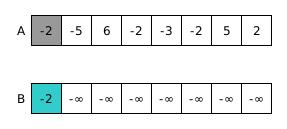
\includegraphics[width=\textwidth]{sources/max_sum_continguous_subarray/images/kadane1}
		\caption{$i=0$: $B[0]$ is equal to the first element of $A$}
		\label{fig:median_sorted_array:kadane0}
	\end{subfigure}
	\hfill
	\begin{subfigure}[t]{0.48\textwidth}
		\centering
		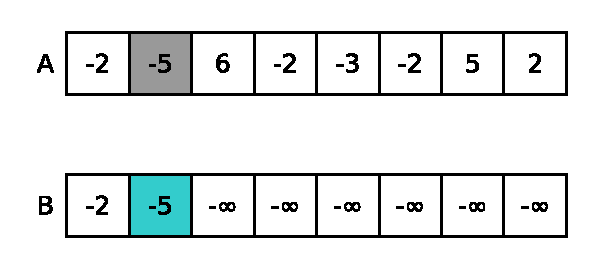
\includegraphics[width=\textwidth]{sources/max_sum_continguous_subarray/images/kadane2}
		\caption{$i=1$: $B[1]$ is equal to $A[1]$ only. $B[0]$ is negative and therefore $B[0]+A[1] < A[1]$.}
		\label{fig:median_sorted_array:kadane1}
	\end{subfigure}
	\hfill

	\begin{subfigure}[t]{0.48\textwidth}
		\centering
		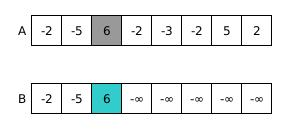
\includegraphics[width=\textwidth]{sources/max_sum_continguous_subarray/images/kadane3}
		\caption{$i=2$: $B[2]$ is equal to $A[2]$ only. $B[1]$ is negative and therefore $B[1]+A[2] < A[2]$.}
		\label{fig:median_sorted_array:kadane2}
	\end{subfigure}
	\hfill
	\begin{subfigure}[t]{0.48\textwidth}
		\centering
		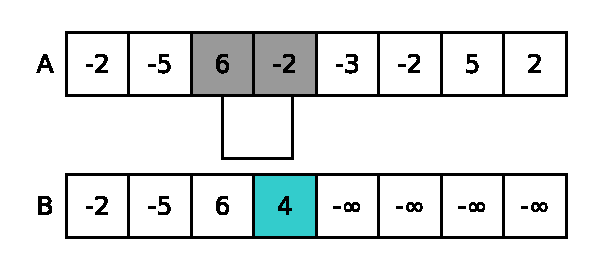
\includegraphics[width=\textwidth]{sources/max_sum_continguous_subarray/images/kadane4}
		\caption{$i=3$: $B[3]$ is equal to $A[2]+A[3]$. $B[2] > 0$ and therefore $B[2]+A[3] > A[3]$.}
		\label{fig:median_sorted_array:kadane3}
	\end{subfigure}
	\hfill

	\begin{subfigure}[t]{0.48\textwidth}
		\centering
		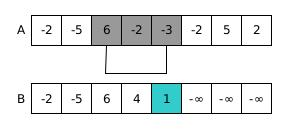
\includegraphics[width=\textwidth]{sources/max_sum_continguous_subarray/images/kadane5}
		\caption{$i=4$: $B[4]$ is equal to $A[3]+A[4]$. $B[3] > 0$ and therefore $B[3]+A[4] > A[3]$.}
		\label{fig:median_sorted_array:kadane4}
	\end{subfigure}
	\hfill
	\begin{subfigure}[t]{0.48\textwidth}
		\centering
		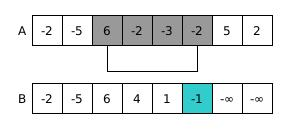
\includegraphics[width=\textwidth]{sources/max_sum_continguous_subarray/images/kadane6}
		\caption{$i=5$: $B[5]$ is equal to $A[4]+A[5]$. $B[4] > 0$ and therefore $B[4]+A[5] > A[5]$}
		\label{fig:median_sorted_array:kadane5}
	\end{subfigure}
	\hfill

	\begin{subfigure}[t]{0.48\textwidth}
		\centering
		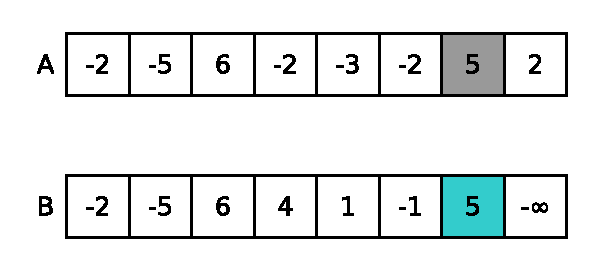
\includegraphics[width=\textwidth]{sources/max_sum_continguous_subarray/images/kadane7}
		\caption{ $i=6$: $B[6]$ is equal to $A[6]$ only. $B[5]$ is negative and therefore $B[5]+A[6] < A[6]$.}
		\label{fig:median_sorted_array:kadane6}
	\end{subfigure}
	\hfill
	\begin{subfigure}[t]{0.48\textwidth}
		\centering
		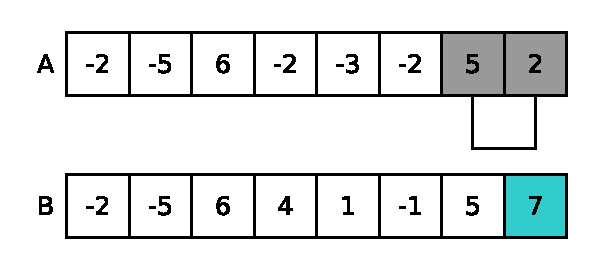
\includegraphics[width=\textwidth]{sources/max_sum_continguous_subarray/images/kadane8}
		\caption{$i=7$: $B[7]$ is equal to $A[6]+A[7]$. $B[6] > 0$ and therefore $B[6]+A[7] > A[7]$ }
		\label{fig:median_sorted_array:kadane7}
	\end{subfigure}
	\caption[Kadane's algorithm.]{This figure shows the array $B$ in the Kadane's algorithm is calculated. Gray cells are part of the sub-array that gives the value to the corrensponding cell in $B$ coloroued in cyan. }
	\label{fig:median_sorted_array:kadane}
\end{figure}


\subsubsection{Linear time and constant space Kadane's algoritm}
But, is the additional space used by $B$ really necessary? A closer look at the implementation of the linear space Kadane's algorithm above provides the answer: no. 

In fact, every value of $B$ is only used \textbf{once}, and then ignored for the rest of the execution (count how many times $B[i]$ is read).
Thus, the algorithm can be modified to take advantage of this fact, so it only uses a single variable to store the latest calculated
value of $B$ i.e. the value for the index $i-1$ as shown in Listing
\ref{list:max_sum_continguous_subarray_kadane}.


\lstinputlisting[language=c++, caption=Constant space and linear time Kadane's algorithm,label=list:max_sum_continguous_subarray_kadane]{sources/max_sum_continguous_subarray/max_sum_continguous_subarray_solution4.cpp}

Notice how the variable \inline{max_ending_here} is doing the job that the variable \inline{B[i-1]}
was doing in the implementation for the linear space Kadane's algorithm, and also how
the final answer is the maximum among all values taken by \inline{max_ending_here}.

The complexity of this approach is $O(n)$ in time and $O(1)$ in space, and very likely is the sort
of complexity the interviewer expects.

\section{Common Variations}
\subsection{Minium sum contiguous sub-array}
A very common variation of this problem is to find the smallest sum instead of the largest. This variation is very quickly solved by just changing the  way the variables in Kadane's algorithm \inline{min_ending_here} (the variable is named \textbf{min} instead of max so to reflect the goal of this variation) and \inline{ans} are updated.
Since the minimum is to be returned, then they should be updated using \inline{min_ending_here = std::min(A[i] , max_ending_here+A[i]);}
and \inline{std::min(ans, in_ending_here)}, respectively.

\subsection{Longest positive/negative contiguous sub-array}
Another common variation of the max/min sum contiguous subarray is to find the longest subarray only containing positive or negative numbers.

The same core behind the Kadane's algorithm can be used for the this variant too. At each iteration $i$ the variable \inline{longest_ending_here} represents the longest
positive subarray up to that iteration and including the element $A[i]$ and can be updated as follows: \inline{longest_ending_here = A[i] >= 0 ? longest_ending_here+1 : 0;}.
%!TEX root = ../main.tex
%%%%%%%%%%%%%%%%%%%%%%%%%%%%%%%%%%
% Links:
%
% Difficulty:
% Companies: 
%%%%%%%%%%%%%%%%%%%%%%%%%%%%%%%%%%

\chapter{String Reverse}
\label{ch:string_reverse}
\section*{Introduction}
Reversing a string is an obiquitous operation and because of that is it very often asked during programming interview. There are basically two variation of this problem:
\begin{enumerate}
  \item in-place.
  \item out-of-place.
\end{enumerate}
and the first thing it should be clarified is which type is the interviewer asking.
Moreover considering the popularity of this problem it is important not to make mistakes and solve the problem in a relatively short time frame. The interviewer most likely is expecting you to have seen this question or solved this challenge yourself more than once in the past.


\section{Problem statement}
The problmen statement is very simple and fits in a single line:
\begin{exercise}
Write a method that takes a string $s$ of length $n$ and reverses it.
\end{exercise}

\begin{example}
	\hfill \\
	Given $s="abcde"$ the function produces $s="edcba"$.
\end{example}

\begin{example}
	\hfill \\
	Given $s="programming"$ the function produces $s="gnimmargorp"$.
\end{example}

\section{Clarification Questions}

\begin{QandA}
	\item Should the function reverses the string in place?
	\begin{answered}
		\textit{Yes, a copy of the input cannot be created.}
	\end{answered}

	\item Is the empty string a valid input?
	\begin{answered}
		\textit{Yes, the input string might be empty.}
	\end{answered}
	
\end{QandA}

\section{Discussion}
\label{string_reverse:sec:discussion}
The problem asks to reverse a string in place. But what does it exactly mean to do it \textit{in-place}? It means that no auxiliary storage is allowed and that the input itself will be processed by the function and will be eventually transformed into the output. Since the original content of the input is lost once the function is terminaed, in-place algorithms are also called \textit{destructive}. Note that no additional storage does not literally mean that not even a single variable can be created. In this case it should be interpreted more as that a copy of the input is disallowed, or that the function should work in $O(1)$ (constant) space.

Let's take a deeper look at what happens to the single letters of the string once they are reversed. For instance consider the string $s="a_0 a_1 a_2 a_3 a_4 a_5"$ which is transformed into $s'="a_5 a_4 a_3 a_2 a_1 a_0"$. The subscript $i$ in $a_i$ identifies the position in which the letter $a_i$ appears in the original input. The core of the problem is to figure our how are letters shuffled from the original to the reversed string. In order to do so one can analyze how the indices are moved during the reverse process. It can clearly be seen from the example above that the indices modifies as follows:
\[
\begin{array}{l}
    0 \rightarrow 5  \\ 
    5 \rightarrow 0  \\ 
    1 \rightarrow 4  \\ 
    4 \rightarrow 1  \\ 
    3 \rightarrow 2  \\ 
    2 \rightarrow 3  \\ 
  \end{array}
\]
The example contains all the information that are necessary to deduce the function that maps the indices of the original string into the indices of the reversed string. An index $i$ gets mappes to an index $j$ s.t. $i+j = n$ (index $0$ goes to $5$). A quick manipulation of that equation shows that $j$ (the index of where the letter at index $i$ in the original string will be in the reversed on) is equal to $j = n-i$. 
This equation effectively says that  each letter at index $i$ in the original input is moved to the $j$'s location.
Also notice from the example above that letter  at index $j$ is itself mapped to index $i$ meaning that letters are positions $i$ and $j$ are effectively swapped.

So to summarize, each character in the input string need to be swapped with its symmetrical sibling (See Listing \ref{list:string_reverse_1}).

\lstinputlisting[language=c++, caption=Iterative solution to the in-place string reverse question.,label=list:string_reverse_1]{/home/dspataro/git/algorithm_articles/sources/string_reverse/string_reverse_solution1.cpp}

Note how the loop terminates at only half the size of the input string. This is necessary because a swap operations on the index $i<\frac{n}{2}$ involves also an element of the second half of the string (its simmetrycal sibling).  If the loop would not terminate at $\frac{n}{2}$ then for each element $i$ two swap operations would be performed. For instacce for the letter at index $0$ the following swaps would occur:
\begin{itemize}
	\item[-] swap(0,n-1)
	\item[-] swap(n-1,0)
\end{itemize}.
Considering that two\footnote{Any even number, to be precise} swap operations on the same indices result in having the original status of the letters (on those indeces) restored, if the loop does not stop at $\frac{n}{2}$ then the function would not modify the original string at all. 


This is considered a good solution because the time and space complexity of Listing \ref{list:string_reverse_1} are $O(n)$ and $O(1)$ respectively, which are optimal. Moreover the solution is short and expressive. 

\section{Common Variation}
\label{string_reverse:sec:variations}

\subsection{Out-of-place solution}
Sometimes the interviewe might ask an easier version of this problem which asks to return a reversed copy of the  original string. This version is easier compared to the in-place version because one can simply construct the reversed string by looping the original string backwards as shown in Listing \ref{list:string_reverse_outplace_rawloop} and Listing \ref{list:string_reverse_outplace_iterators}.

\lstinputlisting[language=c++, caption=Iterative out-of-place solution using raw loops. Both time and space complexity for this version is $O(n)$.,label=list:string_reverse_outplace_rawloop]{/home/dspataro/git/algorithm_articles/sources/string_reverse/string_reverse_solution2.cpp}

\lstinputlisting[language=c++, caption=Alternative implementation of an iterative out-of-place solution using iterators. Both time and space complexity for this version is $O(n)$.,label=list:string_reverse_outplace_iterators]{/home/dspataro/git/algorithm_articles/sources/string_reverse/string_reverse_solution3.cpp}

\subsection{Recursive solution}
Another commonly asked variation of the string reverse problem is the one in which recursion has to be used. The problem is well suited for recursion infact, a look at the iterative solution shows that at any given point in the loop the status of the string is the following: $a_{n-1}a_{n-2} \ldots \underbrace{a_k a_{k+1} \ldots a_l}_\text{untouched} a_{k-1}a_{k-2} \ldots a_0$. There is always a portion of the string delimited by two indices $k$ and $l$, $k>=l$ which is yet to be processed (i.e. with the original content). This can be easily used to derive a recursive solution. At first the $k=0$ and $l=n-1$ and the string can be reversed by swapping $a_k=0$ and $a_l=n-1$ and by recursively reversing the inner part of the string i.e. in the range $k=1$ and $l=n-2$. This can be continuosly be done until $l > k$. At that point the function can simply terminate (See Equation \ref{eq:string_reversal_recursion} and Listing \ref{list:string_reversal_recursion}).

\begin{equation}
	R(s, k, l)=\begin{cases} 
\text{swap}(s[k]s[l]) \: \wedge \: R(s,k+1, l-1) & \text{if } k\geq l\\
\text{return} & \text{otherwise}
\end{cases}
\label{eq:string_reversal_recursion}
\end{equation} 

The complexity analysis for this case can be a bit controversial because one have to consider also the stack space utilized by the recursion which can be $O(n)$. It is therefore important to clarify this aspect with the interviewer. Discussing this might open the possibility for questions related to this, especially regarding Tail Call Optimization(TCO)\footnote{TCO (Tail Call Optimization) is the process by which a smart compiler can make a call to a function and take no additional stack space.The allocation of a new stack frame for a function can be avoided because the calling function will simply return the value that it gets from the called function. The most common use is tail-recursion, where a recursive function written to take advantage of tail-call optimization can use constant stack space.\nopagebreak}, so one needs to be careful while opening this pandora box.

\lstinputlisting[language=c++, caption=Recursive in-place solution to the string reversal problem.,label=list:string_reversal_recursion]{/home/dspataro/git/algorithm_articles/sources/string_reverse/string_reverse_solution4.cpp}
%!TEX root = ../main.tex
%%%%%%%%%%%%%%%%%%%%%%%%%%%%%%%%%%
% Links:
%
% Difficulty:
% Companies: 
%%%%%%%%%%%%%%%%%%%%%%%%%%%%%%%%%%

\chapter{Find the odd occurring element}
\label{ch:find_odd_occurring_element}
\section*{Introduction}

In this chapter we will deal with  a problem on arrays and on the XOR (also known as \textit{disjunctive-or} and usually identified by the symbol
$\oplus$)\footnote{
	$\oplus$ is a boolean binary operator that returns true only when its two inputs have different values i.e. when one is true and the other is false.} 
operation.

There is a very simple, intuitive yet inefficient brute-force solution to the problem, however, as it is conceptually very different from other, faster, approaches it is difficult to use even as a starting point during interview to iteratively improve on to reach optimal time and space complexity.  In this instance, it is more effective to begin by reading the problem statement carefully and looking for the right insight immediately rather than getting carried away towards a dead-end by the brute-force approach.

\section{Problem statement}
\begin{exercise}
Write a function that, given an array $A$ of positive integers where all elements except one appear an even number of times, returns the one and only one element appearing an odd number of times.

	\begin{example}
		\label{ex:find_odd_occurring_element:example1}
		\hfill \\
		Given the array $A=\{4,3,6,2,4,2,3,4,3,3,6\}$ the function returns $4$ because it appears $3$ times while all the other elements appear an even number of times.
		
	\end{example}
\end{exercise}


\section{Clarification Questions}

\begin{QandA}
	\begin{questionitem} \begin{question} Is the input array always valid. Does it always contain only one element appearing an odd number of times?  \end{question} 	 
    \begin{answered}
		\textit{Yes the input array can be assumed to be valid.}
	\end{answered} \end{questionitem}
	\begin{questionitem} \begin{question} Is the range of the input integers known?\footnote{This is very good question because if the answer is yes we can use an approach similar to the counting sort to keep track using only constant space and linear time, of the number of times an element appears.}  \end{question} 	 
    \begin{answered}
		\textit{No it is not. The values of the elements of $A$ is arbitrary.}
	\end{answered} \end{questionitem}
	
\end{QandA}

\section{Discussion}

\subsection{Brute-force}
\label{find_odd_occurring_element:sec:bruteforce}

As mentioned above, the brute-force solution to this problem is very intuitive.  We simply have to count the occurrences of each of the elements of $A$ until we find one appearing an odd number of times.  
Provided that a counting function (which counts the occurrences of a given element in an array) is available, it is only a matter of using that function for all the elements in the array, and return as soon as it returns an odd number. 

Listing \ref{list:find_odd_occurring_element_bruteforce_rawloop} shows a possible implementation in C++ which uses the \inline{std::count} function from the STL to count the number of occurrences of a given number in $A$.


\lstinputlisting[language=c++, caption=Brute force solution using a counting function.,label=list:find_odd_occurring_element_bruteforce_rawloop]{sources/find_odd_occurring_element/find_odd_occurring_element_solution1.cpp}

What the code above is really trying to do is \textbf{find} the element appearing an odd number of times.
Instead of using a raw loop for doing so, the code can be made much more expressive (which is always appreciated  by interviewers) by using the standard \inline{find\_if} metafunction  as shown in the Listing \ref{list:find_odd_occurring_element_bruteforce_standard}.


\lstinputlisting[language=c++, caption=Brute force solution using standard libraries functions \inline{std::count} and \inline{std::find_if}.,label=list:find_odd_occurring_element_bruteforce_standard]{sources/find_odd_occurring_element/find_odd_occurring_element_solution2.cpp}

This is, however, a poor solution as the time complexity is $O(n^2)$ which is far from optimal, while the space complexity is constant. 


Note that, in the first brute-force solution (Listing \ref{list:find_odd_occurring_element_bruteforce_standard}), we dereference the iterator returned by \inline{find\_if} directly without checking if it is valid or not. 
\inline{find_if( InputIt first, InputIt last,UnaryPredicate p)} returns an iterator to the element satisfying the search criteria $p$ (in the form of a lambda)  only if such an element exists, and that otherwise it would return \inline{last} which is  equal to \inline{std::end(A)}.
Dereferencing \inline{std::end(A)} would cause UB, but we can guarantee this won't happen as an odd occurring element is \textbf{always present} in $A$\footnote{How could we change Listing \ref{list:find_odd_occurring_element_bruteforce_standard} so that it handles bad input safely?}.


In the second implementation (Listing \ref{list:find_odd_occurring_element_bruteforce_rawloop}), we took a different approach to handling a bad input and decided to explicitly throw an exception in case all elements appear an even number of times or $A$ is empty. 
Even if the interviewer does not ask for this, it is good to show that we thought about this and also that we can handle it without big penalties in expressiveness and performance: we can rest assured this certainly adds a bonus point to our final evaluation. 
Moreover, we can argue that a throw statement makes it explicit that the function is expecting certain characteristics from the input without incurring performance penalties: \footnote{Throwing an exception is cheap when the exception is not raised. This is the case in the main exception model used nowadays (Itanium ABI, VC++ 64 bits Zero-Cost model exceptions)\cite{cit:web:openstd_exception}.)} when the input is  good
(which is safe to assume would be the majority of the times the function gets invoked).

\subsection{Linear time and space solution}
\label{find_odd_occurring_element:sec:map}

In order to speed up the process of keeping count of how many times each element appear in the input array, we can adopt a map-like structure where the keys are the numbers in $A$ and the values are integers representing the number of times each element appears in the array.
If a hash-based map is used to store this key-value information then this effectively reduces the time complexity of the brute-force approach down to $O(n)$ (on average) at the expense of space that increases to linear as well.

Keeping track of the actual number of times an element appears in $A$ is actually unnecessary as all we need is the information about whether or not the number of times it appears is even or odd. We do not care about the actual number  therefore a single bit is sufficient to store this information. The map structure would then associate integers to booleans for a substantial saving in the space used. However big the reduction is the space used remains linear. 
This idea is implemented in Listing \ref{list:find_odd_occurring_element_bruteforce_linearspace}.

\lstinputlisting[language=c++, caption=Linear time and space solution using a map.,label=list:find_odd_occurring_element_bruteforce_linearspace]{sources/find_odd_occurring_element/find_odd_occurring_element_solution3.cpp}

The code works in two phases:
\begin{enumerate}
	\item the map \inline{M} is filled in such a way that for each key $x$ the corresponding value is $1$ if and only if $x$ appears in $A$ an odd number of times.
	\item the map is scanned to find the one element having a value of $1$.
\end{enumerate}
The time and space complexity are $O(n)$.

\subsection{Linear time and constant space solution}
\label{find_odd_occurring_element:sec:constant_space}

However, there is a way to solve this problem in constant space and linear time. 
This solution is based on the XOR operation which can be thought of as the equivalent of the sum for bits and has several interesting properties that are useful in constructing a solution to this problem:
\begin{enumerate}
	\item it is a commutative, distributive and associative operation;
	\item its neutral element is the $0$. What it means is that applying the XOR to a number $x \neq 0$ and $0$  always results in $x$ i.e. $x \oplus 0 = x$ and $0 \oplus x = x$
	\item xor-ing an element with itself always results in 0 i.e. $x \oplus x = 0$.
\end{enumerate}
The practical consequence of these facts is that when xor-ing an element $x$ with itself an odd number of times, the result is $x$ as $(x \oplus x) \oplus x  = (0 \oplus x) = x$, but doing so an even number of times results in $0$ because  $(x \oplus x) \oplus (x \oplus x) = 0 \oplus 0 = 0$.

This is useful because we known that all input integers except one are occurring an even number of times,  therefore when all numbers are xor-ed together, all that is left at the end is the number appearing an odd number of times: every number except the answer will be xor-ed an even number of times with itself, resulting in $0$. 


For instance if we try to XOR all the elements of the example \ref{ex:find_odd_occurring_element:example1} above where $A=\{4,3,6,2,4,2,3,4,3,3,6\}$ we obtain: $4 \oplus 3 \oplus  6 \oplus 2 \oplus 4 \oplus 2 \oplus 3 \oplus 4 \oplus 3 \oplus 3 \oplus 6 = 4$. At this point we can use commutativity, associativity and distributivity properties to rearrange it as follows (this would be equivalent to first sort $A$ and then XOR all the elements): 
$$\underbrace{(2 \oplus 2)}_{0} \oplus \underbrace{(3 \oplus 3 \oplus 3 \oplus 3)}_{0} \oplus \underbrace{(4 \oplus 4 \oplus 4)}_{4} \oplus \underbrace{(6 \oplus 6)}_{0} = 4$$ which clearly show the only value remaining is the one of the element appearing an odd number of times.


An implementation of the idea above is shown in Listings \ref{list:find_odd_occurring_element_bruteforce_final1} where we explicitly loop over $A$ and \ref{list:find_odd_occurring_element_bruteforce_final2} where instead, we use \inline{std::accumulate} to perform the array reduction\footnote{
	The process of reducing the array to a single value. Can be thought of as an aggregation of the values of an array that results in a single value. The terms reduction comes from the fact that this operation in its general form can be applied to a multi-dimensional object (imagine a 3D matrix for instance)  which are aggregated across a dimension and results in a value without that dimension (into a 2D matrix), practically reducing the number of dimensions of that object by one. In the case of an array, we go from a one-dimensional object to a scalar. Calculating the average, sum, or variance of an array are all examples of reduction operations.}.

\lstinputlisting[language=c++, caption=Linear time and constnat space using XOR and a raw loop.,label=list:find_odd_occurring_element_bruteforce_final1]{sources/find_odd_occurring_element/find_odd_occurring_element_solution4.cpp}


\lstinputlisting[language=c++, caption=Linear time and constant space solution using XOR $\oplus$ and the \inline{std::accumulate} function from the STL.,label=list:find_odd_occurring_element_bruteforce_final2]{sources/find_odd_occurring_element/find_odd_occurring_element_solution5.cpp}

Both implementations \ref{list:find_odd_occurring_element_bruteforce_final1} and \ref{list:find_odd_occurring_element_bruteforce_final2} have very similar characteristics in terms of asymptotic performance, as they both use linear time and constant space. 
%!TEX root = ../main.tex
%%%%%%%%%%%%%%%%%%%%%%%%%%%%%%%%%%
% Links:
%
% Difficulty:
% Companies: 
%%%%%%%%%%%%%%%%%%%%%%%%%%%%%%%%%%

\chapter{Capitalize the first letters of every words}
\label{ch:capitalize_words_first_letter}
\section*{Introduction}
Editing text is probably one of the most basic and common operations computers are nowadays still used for. There are a huge number of editors out there, some of them are specialized for a particular kind of users (think of the zoo of editors a programmer can choose from e.g.
\begin{enumerate*}
	\item vi,
	\item GNU Emacs,
	\item gedit,
	\item TextPad,
	\item Visual Studio Code,
	\item Eclipse,
	\item Sublime Text,
	\item Qt Creator,
	\item etc.
\end{enumerate*}
) while others are intended to be for a broader audience like MS Word or LibreOffice writer. 

Imagine for a second to be a software engineer working on a feature for the new version of Word that is supposed to make the tedious tasks of converting a particular piece of text into a variant of the "title case"\footnote{All words are capitalized, except non-initial articles like “a, the, and”, etc.}.
The idea is that the user would highlight a portion of text and then have the text modified in place by simply pressing a button instead of manually changing every single letter. Implementing such feature is often part of preliminary stages interviews and it is used as a warm-up problem mostly due to its simplicity. 
In this chapter, we will discuss how the core such feature can be implemented and we will have a look at a number of possible implementations and solutions approaches. This problem is not hard and therefore the focus of this chapter is more on making sure the final solution is readable and easy to understand rather than coming up with a fancy algorithm.

\section{Problem statement}
\begin{exercise}
Write a function that given a string $s$, modifies it so that every first letter of every word in $s$ is in upper case while leaving the rest of the characters untouched.

	\begin{example}
		\hfill \\
		Given the string \verb\"arturo benedetti michelangeli is the best pianist ever\". The function should turn it into: \verb\"Arturo Benedetti Michelangeli Is The Best Pianist Ever\"\footnote{A.B.M (5 January 1920 - 12 June 1995) was an Italian classical pianist considered as one of the greatest pianists of all times. He was perhaps the most reclusive, enigmatic and obsessive among the handful of the world's legendary pianists.}
	\end{example}

	\begin{example}
		\hfill \\
		Given the string:
		\begin{verbatim}
			"Truth May Seem BUt Cannot be;
			Beauty brag but ’tis not she;
			TruTh and beauty buried be."
		\end{verbatim}
		The function should turn it into: 
		\begin{verbatim}
			"Truth May Seem BUt Cannot Be;
			Beauty Brag But ’tis Not She;
			TruTh And Beauty Buried Be."
		\end{verbatim}
	\end{example}
	
\end{exercise}
	
\section{Discussion}
\label{capitalize_words_first_letter:sec:discussion}
This problem does not require coming up with a fancy and complicated algorithm in order to clear the interview.
The idea behind solving this problem is more about showing you can put together a working implementation in a relatively short amount of time and spend the rest of the time polishing it so that it is clean, readable and easy to understand.

What are the practical implications of having to capitalize only the first letter of every word? Let's start by first looking at what makes a letter the \textbf{first} letter of a word. 
A character is the beginning of a word if any of the following is true:
\begin{itemize}
	\item it is not space and it is preceded by a space,
	\item it is not space and it is the first character of the string.
\end{itemize}
Any other character is either a space (for which the notion of lower/upper case does not make much sense) or it is in the middle of a word i.e. surrounded by other letters. Given this definition, all it is necessary to do to solve this problem is to search for any character in the input string satisfying any of the criteria above as shown in Listing \ref{list:capitalize_words_first_letter_simple}.

\lstinputlisting[language=c++, caption=Linear time constant space solution.,label=list:capitalize_words_first_letter_simple]{sources/capitalize_words_first_letter/capitalize_words_first_letter_solution4.cpp}

Listing \ref{list:capitalize_words_first_letter_simple} works in two phases:
\begin{enumerate}
	\item make sure that the first character of $s$ is handled properly (depending on whether it is a space or not),
	\item takes care of the rest of the characters from the position $1$ (skipping the very first one) onward.
\end{enumerate}

\subsubsection{\texttt{std::adjacent\_find}}
The very same idea discussed above and shown in Listing \ref{list:capitalize_words_first_letter_simple} can be implemented using the function \inline{std::adjacent_find}\cite{cit::std::adjancefind} from the STL which can be used to search, in a range, for a pair of subsequent elements satisfying  a user-provided criteria. In the context of this solution, we can use it to find all pairs composed by a space followed by a letter, which we know is the letter that has to be capitalized as it marks the beginning of a word.
Listing \ref{list:capitalize_words_first_letter_adj_find} implements this idea. 

\lstinputlisting[language=c++, caption=Linear time constant space solution using \href{https://en.cppreference.com/w/cpp/algorithm/adjacent_find}{\texttt{std::adjacent\_find}}\cite{cit::std::adjancefind}. by,label=list:capitalize_words_first_letter_adj_find]{sources/capitalize_words_first_letter/capitalize_words_first_letter_solution2.cpp}

The complexity of the Listing \ref{list:capitalize_words_first_letter_adj_find}  is linear in time and constant in space and it has the same asymptotical complexity profile as the one presented in Listing \ref{list:capitalize_words_first_letter_simple} with the added benefit of being more expressive as the code explicitly uses the definition of "first letter of a word" given above.

\subsubsection{Recursive solution}

Another way of looking at solving this problem is by adopting a recursive approach like the following: 
\begin{enumerate}
	\item find the first character in the string 
	\item transform it in uppercase,
	\item ignores all the subsequence non-space characters until a space or the end of the string is reached.
\end{enumerate}
When we hit a space, we repeat the process from the beginning, otherwise we stop as at this point the whole string is modified so that only the first character of every word is in uppercase and the rest of the string is untouched.
Listing \ref{list:capitalize_words_first_letter_iterator} shows how the steps above con be turned into a working solution. 

\lstinputlisting[language=c++, caption=Linear time constant space solution. ,label=list:capitalize_words_first_letter_iterator]{sources/capitalize_words_first_letter/capitalize_words_first_letter_solution1.cpp}

The code is clearly divided into three distinct blocks each performing one of the tasks listed above (see code comments).
The variable \inline{it} is an iterator pointing to the  element currently under examination and it is used by the outer loop to determine whether the string has been completely processed.
\inline{it} is moved inside the body of the loop which, by processing the text from left to right, ignores all spaces until a letter is found (first inner loop). Such a letter is then is capitalized, and then \inline{it} is moved forward so that all the non-space intra-words characters are ignored (second inner loop). This process repeats until the text is fully processed. 

Notice how we use short-circuit evaluation\footnote{
	Also known as \textit{minimal evaluation} or \textit{McCarthy evaluation}, refers to the semantic of certain boolean operators in which the second argument is executed or evaluated only if the first argument does not suffice to determine the value of the expression.}\cite{cit:wiki:shortcircuit}
in the \inline{while (it != end(s) && *it == ' ')} expression so to always be sure \inline{it} is pointing to a valid element when we dereference it.

The complexity of this solution is linear in time, as every letter is read or modified at most once. The space complexity is constant.



\section{Common Variations}
\label{capitalize_words_first_letter:sec:variation}

\subsection{Apply an user provided function}
Sometimes this problem can be posed such that the operation to be applied on the letter is different than capitalization or alternatively, you can be even asked to write a high order function that takes the operation to be performed as an additional parameter (as a lambda for instance).

We can use the same core ideas discussed above even if we decided to go for a generic solution where we accept a function from the user. The complications are only syntactical as shown in 
Listing \ref{list:capitalize_words_first_letter_userdefined} that shows a generic solution can be implemented. The code takes as an input a string and (in addition to the code code the other solutions discussed above), a function \inline{char f(char)} that takes as an input a character and returns a character. This function is used in place of the \inline{std::to_upper}.

\lstinputlisting[language=c++, caption=Generic version of Listing \ref{list:capitalize_words_first_letter_adj_find},label=list:capitalize_words_first_letter_userdefined]{sources/capitalize_words_first_letter/capitalize_words_first_letter_solution3.cpp}

\subsection{Modify the every $k^{th}$ character of every word}
Another common variation is one where we need to modify every $k^{th}$ character of a word (if it exists). For instance, you might be asked to:

\begin{exercise}
Given a string $s$, modify $s$ such that every $3^{rd}$ letter of every word in $s$ is modified according to a function provided by the user. The rest of the string should remain untouched.
\end{exercise}

This variation can be solved by using Listing \ref{list:capitalize_words_first_letter_iterator} as a starting point and the actual implementation is left as exercise for the reader.



%!TEX root = ../main.tex
%%%%%%%%%%%%%%%%%%%%%%%%%%%%%%%%%%
% Links:
%
% Difficulty:
% Companies: 
%%%%%%%%%%%%%%%%%%%%%%%%%%%%%%%%%%

\chapter{Trapping Water}
\label{ch:trapping_water}
\section*{Introduction}
Imagine being the only survivor of a plane crash in the middle of the pacific ocean and that you managed to get ashore to the Manra Island\footnote{Also called Sydney Island, is almost entirely of scrub forest, herbs, and grasses. The island is abandoned since 1963. 
%\vspace{-0.5cm}
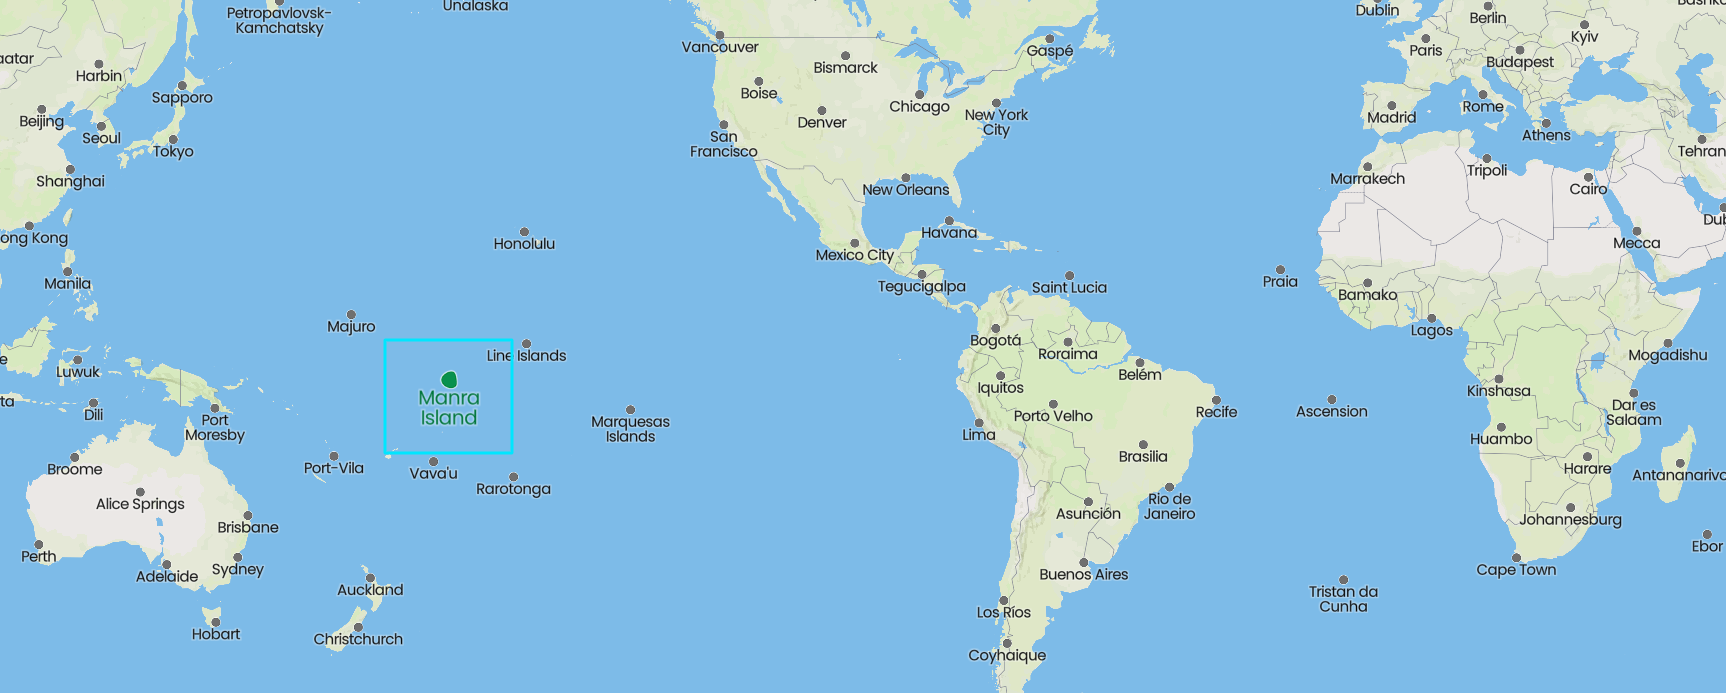
\includegraphics[]{sources/trapping_water/images/manra_island}} 
and that the only cargo item surviving the crash was a large number of plastic cubic boxes of size $1m^3$ and, two long, wide, and rigid sheets of acrylic glass \footnote{Poly (methyl methacrylate) (PMMA), is a transparent thermoplastic often used in sheet form as a lightweight or shatter-resistant alternative to glass.}.

Clearly one of your first worries would be to make sure you have enough water to be able to survive long enough for rescuers to find and save you.
You come up with the brilliant idea of arranging the boxes into piles of different heights each placed along the same direction  
at a certain distance from each other so that they form concave structures that sealed with the help of the plastic sheets collect rainwater as depicted in Figure \ref{fig:trapping_water_example1}. 

In order to figure out the best ways of arranging boxes so that the structure collects as much water as possible to take advantage of the scarce rain, you would like to calculate the total amount of water each possible boxes arrangement can hold.
In this chapter's problem we will investigate how this calculation can be carried out efficiently and, as we shall see, we will learn that there are a number of valid approaches that can be used.
We believe it is important to master the core concepts of all of them as their applicability extends further to the limited context of this specific problem and that, we can extract valuable lessons from each of them.
Moreover, this problems has been (and according to what interviewees across the globe still reports) a major hit in top tech companies, where it is still nowadays frequently asked during interviews.


\section{Problem statement}
\begin{exercise}
Write a function that takes as input an array of length $n$ of non-negative integers representing an elevation map (the height of each pile of boxes) where the width of each bar is $1$. 
The function should return the maximum amount of water that can be potentially trapped in between all the piles. 

	\begin{example}
		\label{ex:trapping_water:exmaple1}
		\hfill \\
		Given the array $H=[0,1,0,2,1,0,1,3,2,1,2,1]$ (see Figure \ref{fig:trapping_water_example1}), the function return $8$
	\end{example}

	\begin{example}
		\label{ex:trapping_water:exmaple2}
		\hfill \\
		Given the array $H=[3,2,0,0,4,4,1,2,5,4,0,2,1]$ (see Figure \ref{fig:trapping_water_example2}), the function return $14$
	\end{example}

\end{exercise}

\begin{figure}
	\centering
	\includegraphics[scale=1.0]{sources/trapping_water/images/example1}
	\caption{Visual representation of the heightmap $H=[0,1,0,2,1,0,1,3,2,1,2,1]$ in the Example \ref{ex:trapping_water:exmaple1}. Blue squares represent water, while the red ones, boxes.}
	\label{fig:trapping_water_example1}
\end{figure}



\begin{figure}
	\centering
	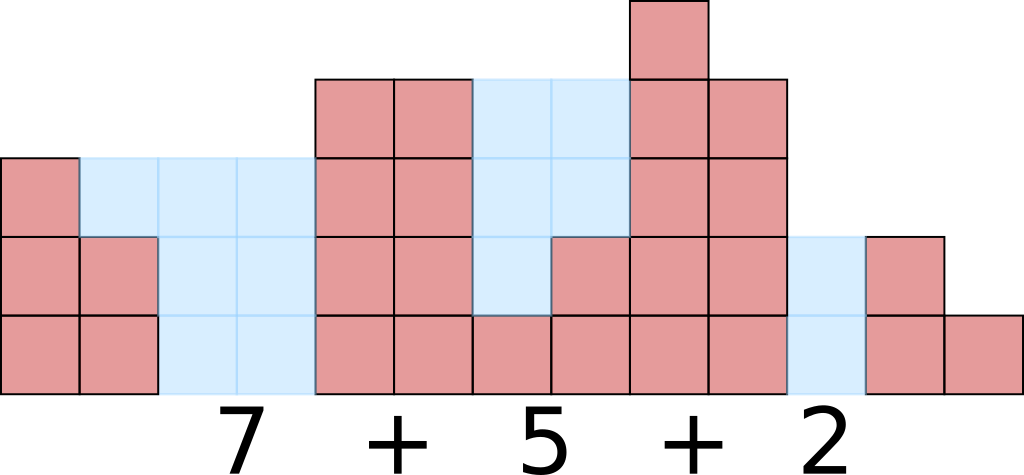
\includegraphics[scale=1.0]{sources/trapping_water/images/example2}
	\caption{Visual representation of the heightmap $H=[3,2,0,0,4,4,1,2,5,4,0,2,1]$ in the Example \ref{ex:trapping_water:exmaple2}. Blue squares represent water, while the red ones, boxes.}
	\label{fig:trapping_water_example2}
\end{figure}

%\section{Clarification Questions}
%
%\begin{QandA}
%	\item 
%	\begin{answered}
%		\textit{}
%	\end{answered}
%	
%\end{QandA}

\section{Discussion}
\label{trapping_water:sec:discussion}
There are at least three tecniques we can use to  solve this challenge so that that will satisfy the interviewer:
\begin{enumerate}
	\item Dynamic programming (Section \ref{trapping_water:sec:dp})
	\item Two pointers (Section \ref{trapping_water:sec:two_pointers})
	\item Stack (Section \ref{trapping_water:sec:stack})
\end{enumerate}
But as usual, we will start our discussion on the problem's solutions by looking at a possible brute-force solution before  passing onto more sophisticated and faster solutions.

\subsection{Brute-force}
\label{trapping_water:sec:bruteforce}

A possible way to brute-force  solve this problem comes from the fact that each element of the array (pile) can potentially hold some water provided that there are other two bars surrounding it (one at its left and one at its right), with height equal or higher.
If that is the case then, we can safely add enough water so its level reaches an height equal to the smallest of the two surrounding piles.
For instance w.r.t. to \ref{ex:trapping_water:exmaple2}, we can see that for the element at index $6$ (having height $1$), the highest bars on its left and right have height $3$ and $4$, respectively. 
We can add water on top of the pile at index $6$ up to a height of $3$ (the minimum between $3$ and $4$) without risking the water spilling out.
Figure \ref{fig:trapping_water_example3} depicts how the pile marked with the question mark can be processed using this approach i.e. by calculating the minimum between $b_l$ and $b_r$ (the height of the highest bars on its left and right, respectively).

If on the other hand, a pile is higher than both the highest bars on its left and right side, then it is impossible to add any water on it (this is the case always the case when processing the highest bar on the histogram).


\begin{figure}
	\centering
	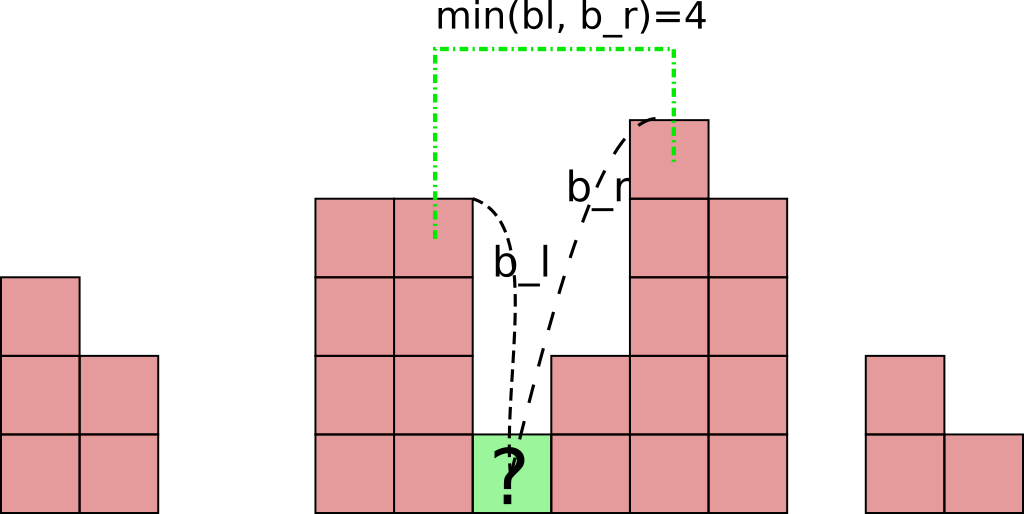
\includegraphics[scale=1.0]{sources/trapping_water/images/example3}
	\caption{Calculation of the water we can fit on top of a pile using the information about the highest bars surrounding it.}
	\label{fig:trapping_water_example3}
\end{figure}

To summarize, we can find the answer to an instance of this problem by calculating the amount of water we can place on top of each pile \inline{H[i]} by:
\begin{enumerate}
	\item find the height of the highest bars on the left (\inline{b_l}) and right (\inline{b_r}) of \inline{H[i]};
	\item add \inline{std::max(0, std::min(b_l, b_r) - H[i])} to the final answer. 
\end{enumerate}
\inline{b_l} and  \inline{b_r} can be implemented with a simple linear search which is performed for all the elements of $H$ causes the complexity of the full algorithm to reach $O(n^2)$.
Moreover, we should notice that the first and the last element will never be able to hold any water as those elements have no bars on their left and right, respectively (any water placed on top of them will inevitably spill outside the structure).

Listing \ref{list:trapping_water:bruteforce} shows a possible implementation of this idea. 
Notice how the \inline{std::max_element} function from C++ STL can be employed elegantly to calculate $b_l$ and $b_r$.

\lstinputlisting[language=c++, caption=Brute-force solution.,label=list:trapping_water:bruteforce]{sources/trapping_water/trapping_water_solution1.cpp}


\subsection{Dynamic Programming}
\label{trapping_water:sec:dp}
The solution proposed in Section \ref{trapping_water:sec:bruteforce} is far from optimal, but it can be transformed into a pretty good one if we can somehow precalculate the values of $b_l$ and $b_r$ in linear time,
We have discussed in great detail how this can be achieved in Chapter \ref{ch:greatest_right}, and it can indeed be accomplished in linear time. 

Therefore all it is necessary is to use pre-calculate (reusing the logic in Listing \ref{list:greatest_right_final1} for instance) $R$, and $L$ each of length $n$ (same as $|H|$) where: 
\begin{itemize}
	\item $R[i]$ contains the value of the highest bar among all elements of the input with index $j > i$ (on the right of, and not considering, $i$).
	\item symmetrically, $L[i]$ contains the value of the highest bar among all elements of the input with index $j < i$ (on the left of, and not considering, $i$).
\end{itemize}

Armed with these two arrays, the same algorithm used in Section \ref{trapping_water:sec:bruteforce} can be turned into an elegant and efficient solution that will make any interviewer smile as shown in 
Listing \ref{list:trapping_water:dp}.

\lstinputlisting[language=c++, caption={Dynamic programming, $O(n)$ time and space solution.},label=list:trapping_water:dp]{sources/trapping_water/trapping_water_solution2.cpp}

The code is clearly divided into two separate and kind of independent steps each of time complexity $O(n)$. 
\begin{enumerate}
	\item vectors \inline{R} and \inline{L} are filled up by using the function \inline{max_left_it}. It is worth noticing here how we are able to calculate $R$ only using the function \inline{max_left_it} (that as hinted by its name calculates the maximum value to the left of each element of the input array), by providing the input to \inline{max_left_it} reversed reversing what comes out of it; Figures \ref{fig:trapping_water_DPL} and \ref{fig:trapping_water_DPR} show a representation of $L$ and $R$. If we superimpose them we can visualize the amount of water we can trap between the piles as shown in  Figure 
	\ref{fig:trapping_water_DPRL}.
	\item the answer calculated by summing up the amount of water that can stand on top of a pile by using the values of  \inline{R[i]}, \inline{L[i]} and \inline{height[i]} as also discussed in Section \ref{trapping_water:sec:discussion}.
\end{enumerate}

Listing \ref{list:trapping_water:dp} has a time complexity of $O(n)$ because the computation of $L$ and $R$ can be done in linear time, while calculating the final answer can be done in a single pass over the array. The space complexity is linear as well because the arrays $L$ and $R$ have both size proportional to $n$.

\begin{figure}
\centering
\begin{subfigure}[b]{0.95\textwidth}
   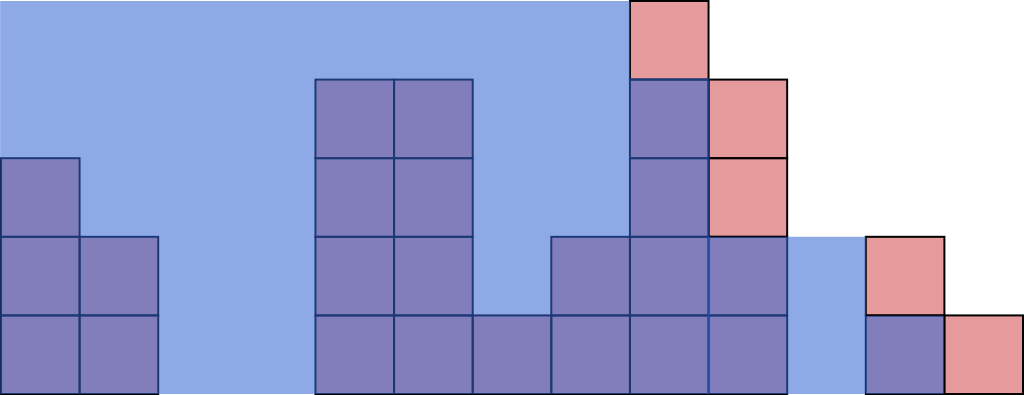
\includegraphics[width=1\linewidth]{sources/trapping_water/images/DPR}
   \caption{Representation of the highest value to the right of a pile. The level of color \textcolor[HTML]{3268d5}{$\blacksquare$} on top of each pile marks the maximum height of another pile to its \textbf{right}.}
   \label{fig:trapping_water_DPL}
\end{subfigure}

\begin{subfigure}[b]{0.95\textwidth}
   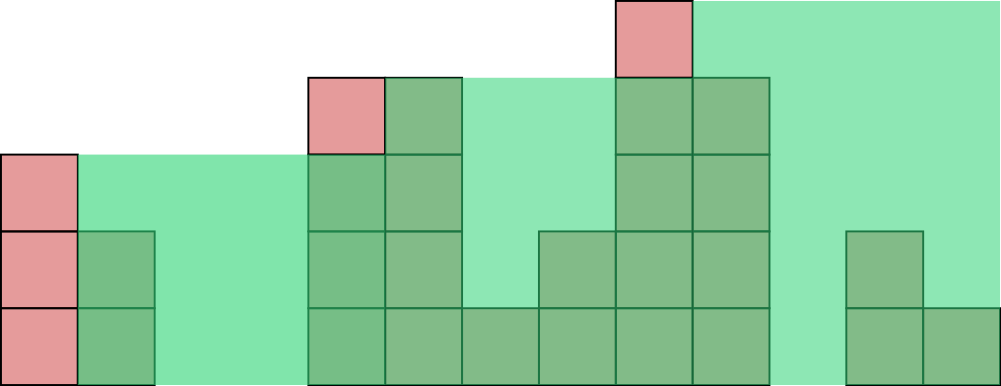
\includegraphics[width=1\linewidth]{sources/trapping_water/images/DPL}
   \caption{Representation of the highest value to the left of a pile. The level of color \textcolor[HTML]{32d579}{$\blacksquare$} on top of each pile marks the maximum height of another pile to its \textbf{left}.}
   \label{fig:trapping_water_DPR}
\end{subfigure}

\begin{subfigure}[b]{0.95\textwidth}
   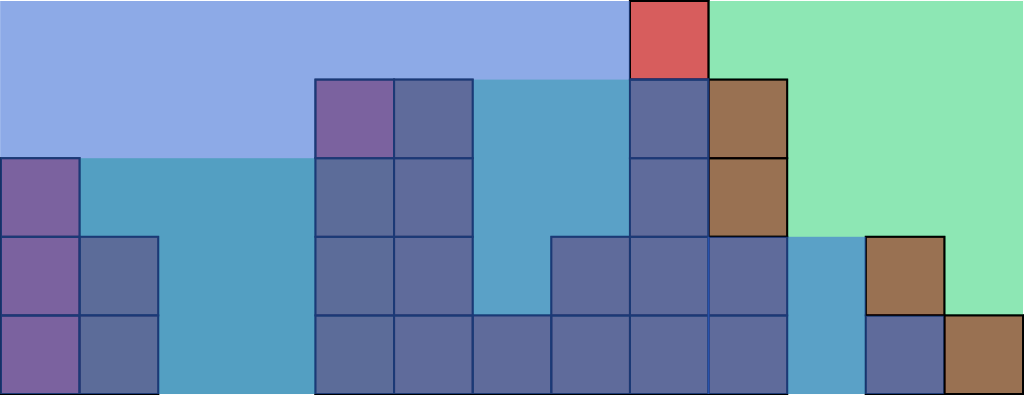
\includegraphics[width=1\linewidth]{sources/trapping_water/images/DPLR}
   \caption{Superimposition of Figures \ref{fig:trapping_water_DPL} and \ref{fig:trapping_water_DPR}. Cells colored in \textcolor[HTML]{5aa1c7}{$\blacksquare$} represent the intersection between cells colored in \textcolor[HTML]{3268d5}{$\blacksquare$} in Figure \ref{fig:trapping_water_DPL} and cells colored in \textcolor[HTML]{32d579}{$\blacksquare$} in Figure \ref{fig:trapping_water_DPR}. Those are the cells that can trap water.}
   \label{fig:trapping_water_DPRL}
\end{subfigure}
\caption{}
\label{fig:trapping_water:dprl_main}
\end{figure}



\subsection{Two pointers solution}
\label{trapping_water:sec:two_pointers}
Despite the fact that the solution presented in Section \ref{trapping_water:sec:dp} is already a good time-complexity-wise, we can definitely do better and lower the space complexity down to $O(1)$.
The key idea is that, we do not really need to store the information of $L$ and $R$ in their entirety.
Whenever we are calculation the contribution of a pile,  we only need a single value from both $L$ and $R$; nothing else.
Once we are done with that pile we can freely discard the corresponding elements in $L$ and $R$ we have used because they are of never to be used in the future as they do not play any role in the calculation of the contribution to the final answer of any other element of the input array $H$.
The solution proposed in this Section uses a two-pointers technique which maintain two \textit{rolling} maximum values, $m_l$ and $m_r$, one for the left and one for the right of a single pile.
When processing the pile at index $i$, $m_l$ and $m_r$ contain the maximum value to the its left and right, respectively (the same information stored in $L[i]$ and $R[i]$).

The input arrays is traversed from left to right using two pointers $l$ and $r$, which are initialized to the beginning and the end of the input array, respectively.
$m_l$ and $m_r$ are initialized to $0$.
The idea is that we process one of the elements pointed by $l$ or $r$ depending on which is larger. 
$m_l$ and $m_r$ always contain the largest element to the left of $l$ and, simmetrically $m_r$ contains the largest element to the right of $r$. 

We process the smallest element between $H[l]$ and $H[r]$ and in particular if \inline{H[l] <= H[r]} is:
\begin{description}
	\item[true:]  then the contribution of \inline{H[l]} is bounded by \inline{m_l} (because \inline{H[r] >= H[l]}. $l$ is moved towards the center (we have considered the contribution of this cell and we can move forward).\\
	\item[false:] then the contribution of \inline{H[j]} is bounded by \inline{m_r} (because \inline{H[l] >= H[r]}. $r$ is moved towards the center (we have considered the contribution of this cell and we can move forward). \\
\end{description}

An implementation of the idea above is shown in Listing \ref{list:trapping_water:two_pointers}.

\lstinputlisting[language=c++, caption={Two pointers solution, $O(n)$ time and  $O(1)$ space, solution to the problem of calculating the amount of water trapped between buildings.},label=list:trapping_water:two_pointers]{sources/trapping_water/trapping_water_solution3.cpp}

The code is pretty self explanatory but it is worth noticing that all the elements of the input array will be  considered eventually because either $l$ or $r$ are moved one one step closer to each other at each iteration. 

This approach has a time complexity of $O(n)$ (we cannot do better than this because at least we have to touch all the elements of the input at least once) and a space complexity of $O(1)$ which is optimal.

We believe this is the solution the interviewer is hoping to see. 


% review done 13/07

\subsection{Stack based solution}
\label{trapping_water:sec:stack}
There is another way of solving this problem in linear time that makes good use of a stack. The main idea is to loop through $H$ one element $p_i$ (pile at index $i$ in $H$) at the time and try to place $p_i$ on the stack in such a way that the values in the stack are always in a decreasing order (from top to bottom).
We start with an empty stack $S$ and for each pile $p_i \in H$ we do one of the two following operations depending on whether $p_i$  is lower than the current top of the stack $s_{top}$:
\begin{description}
	\item[$p_i < s_{top}$] the current top of the stack is higher than $p_i$ which means that $s_{top}$ bounds $p_i$ from the left. In this case we simply add it to the top of the stack. At this point the stack is still ordered in a decreasing fashion.
	\item[$p_i \geq s_{top}$] we have a pile that is higher or equal to the $s_{top}$. Therefore if we want to place $p_i$ on the stack and maintain the ordering, we need to remove as many elements as necessary until we are left with a top of the stack that is higher of $p_i$, or the stack is fully empty (this happens for instance, but not only, when $p_i$ is the highest pile in $H$).
	However each each pile that is removed together with $p_i$  form a rectangular area that can trap some water. Why is that? Well, the removed pile is bounded from the left by some other pile (this is guaranteed by how elements are inserted in the stack, or more simply by the ordering the stack maintains) and to the right by $p_i$ itself. 
	How much water exactly? 
	The contribution of the removed element $S_{oldtop}$ is calculated as the area of a rectangle of base equal to the distance between the two bounding bars ($p_i$ and the element before $S_{oldtop}$) and and height that is equal to the minimum of the heights between the two bounding bars \textbf{minus} $S_{oldtop}$. Clearly if there is no bar left in the stack once we remove $S_{oldtop}$, there is no way we can trap water and therefore we add nothing to the final answer. 
\end{description}
Figure \ref{fig:trapping_water:stack_ex} shows a step-by-step  execution of this algorithm.

A possible implementation of this idea is shown in Listing \ref{list:trapping_water:stack}.
Notice that the real work happens inside the \inline{while} loop and that the pile we calculate the contribution is named \inline{old_top} while the bar on the left and right are named \inline{bar_left} and \inline{bar_right} (equivalent to $p_i$) respectively. 
Moreover, no matter the stack is unwound or not, \inline{bar_right} is \textbf{added} to the stack because when controls reaches line $21$ it will be either the only bar in the stack of it will be smaller than the current top (order is restored).



The complexity of this approach is linear in both time and space .

\lstinputlisting[language=c++, caption={Stack based solution, $O(n)$ time and  space solution.},label=list:trapping_water:stack]{sources/trapping_water/trapping_water_solution4.cpp}

 


\begin{figure}
	\vspace{-0.4in}
	%\hspace*{-0.3in}
	\centering
	\begin{subfigure}[t]{0.24\textwidth}
		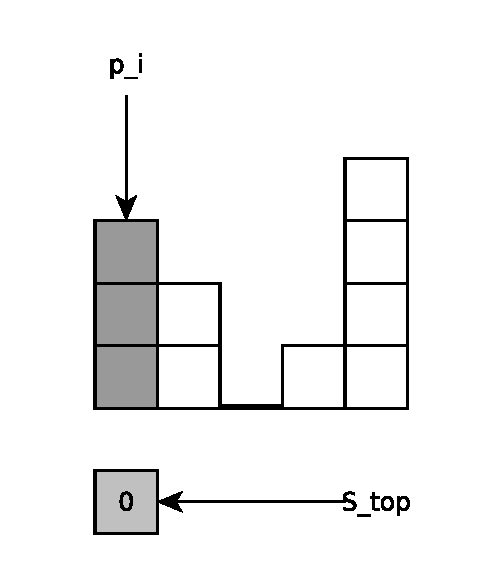
\includegraphics[width=1\linewidth]{sources/trapping_water/images/stack_ex1}
		\caption{At the beginning the stack is empty and pile $0$ is pushed onto it.}
		\label{fig:trapping_water:stack_ex1}
	 \end{subfigure}
	\hfill
	\begin{subfigure}[t]{0.24\textwidth}
		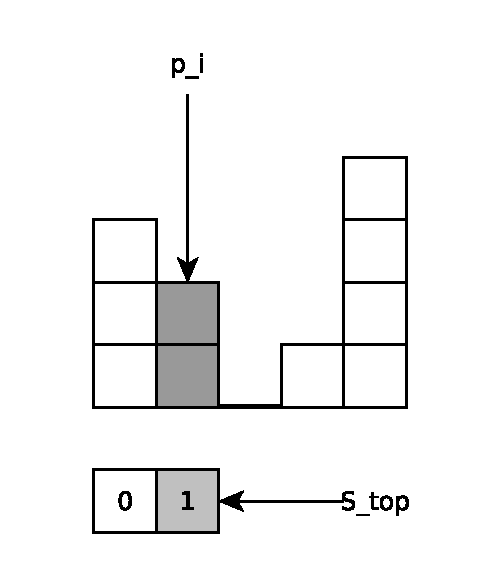
\includegraphics[width=1\linewidth]{sources/trapping_water/images/stack_ex2}
		\caption{Pile  at index $1$ is 2 boxes tall and it is smaller than the current top of the stack having height equal to $3$. Pile $1$ is pushed onto the stack.}
		\label{fig:trapping_water:stack_ex2}
	 \end{subfigure}
	 \hfill
	 \begin{subfigure}[t]{0.24\textwidth}
		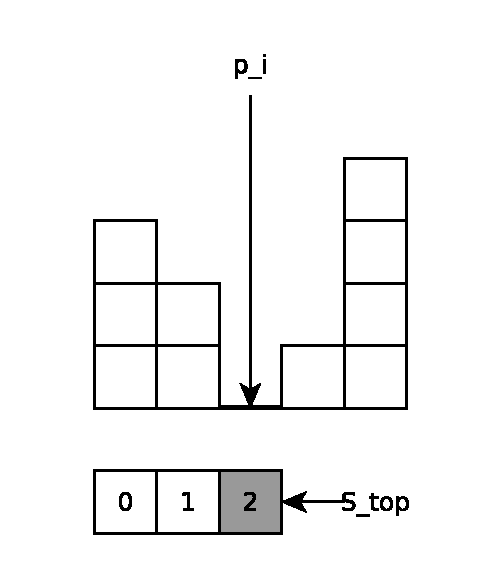
\includegraphics[width=1\linewidth]{sources/trapping_water/images/stack_ex3}
		\caption{Pile $2$ has height $0$ which is smaller than the top of the stack and it is thus pushed on top.}
		\label{fig:trapping_water:stack_ex3}
	 \end{subfigure}
	 \hfill
	 \begin{subfigure}[t]{0.24\textwidth}
		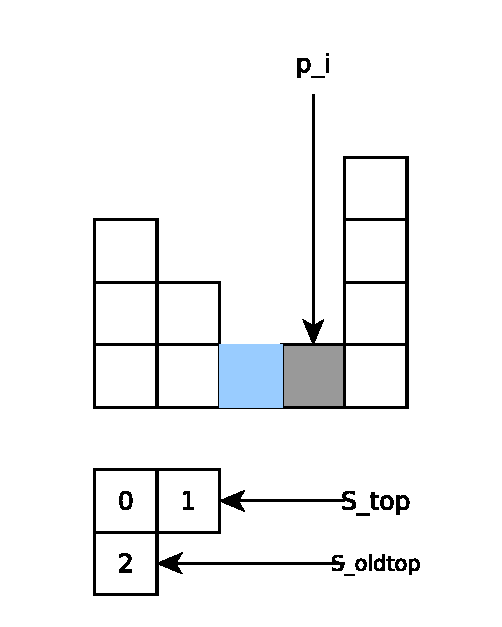
\includegraphics[width=1\linewidth]{sources/trapping_water/images/stack_ex4}
		\caption{Pile $3$ has height $1$ which is higher than the current top of the stack. We therefore pop the current top (we store it in $S_{oldtop}$) and we calculate its contribution to the final answer by using it, the new top and $p_i$. The area that can be filled with water is highlighed in light blue \textcolor[HTML]{99ccff}{$\blacksquare$}. At this point the new top is higher than $p_i$ and we can push it onto the stack which now contains $\{0,1,3\}$.}
		\label{fig:trapping_water:stack_ex3}
	 \end{subfigure}
	 \hspace*{-0.5in}
	 \begin{subfigure}[t]{0.24\textwidth}
		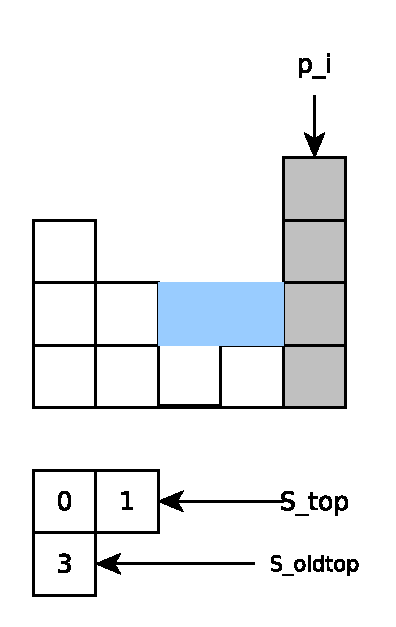
\includegraphics[width=1\linewidth]{sources/trapping_water/images/stack_ex5}
		\caption{The last pile is the highest of all and therefore it is also taller than the top of the stack. We pop the current top pile $3$ of height $1$ and we calculate its contribution to the final answer; an area of two squares in this case (highlighed in light blue \textcolor[HTML]{99ccff}{$\blacksquare$}).}
		\label{fig:trapping_water:stack_ex3}
	 \end{subfigure}
	 \hfill
	 \begin{subfigure}[t]{0.24\textwidth}
		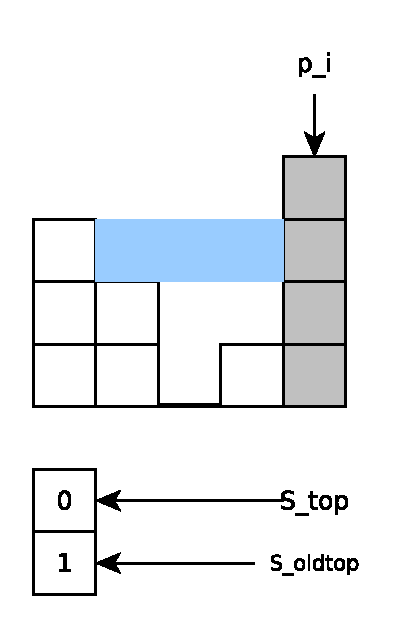
\includegraphics[width=1\linewidth]{sources/trapping_water/images/stack_ex6}
		\caption{At this point we are still trying to insert pile $4$ onto the stack, but its height is still higher than the current top of the pile (pile $1$ of height $2$). Therefore, we pop the current top and calculate its contribution to the final answer (the three cells highlighed in lighe blue \textcolor[HTML]{99ccff}{$\blacksquare$}).}
		\label{fig:trapping_water:stack_ex3}
	 \end{subfigure}
	 \hfill
	 \begin{subfigure}[t]{0.24\textwidth}
		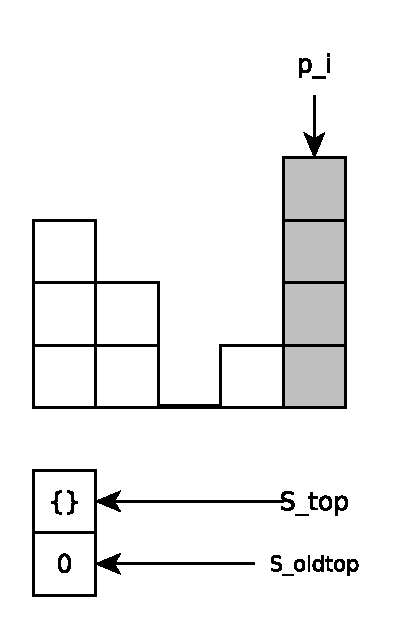
\includegraphics[width=1\linewidth]{sources/trapping_water/images/stack_ex7}
		\caption{At this point there is only one element in the stack (pile $0$) which happens to be smaller then $p_i$. We therefore move the current top to $S_{oldtop}$ and we would normally calculate its contribution to the final answer, but at this point the stack is empty which means pile $0$ is not bound by any other pile to the left. $p_i=4$ is finally added to the stack.}
		\label{fig:trapping_water:stack_ex3}
	 \end{subfigure}
	 \hfill
	 \begin{subfigure}[t]{0.24\textwidth}
		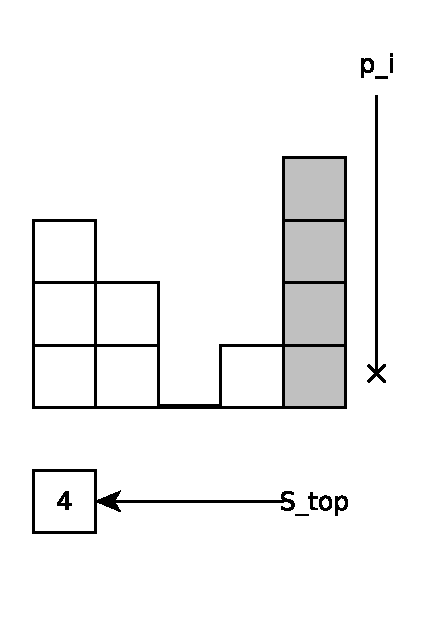
\includegraphics[width=1\linewidth]{sources/trapping_water/images/stack_ex8}
		\caption{At this point the algorithm terminates as there is no more pile to process.}
		\label{fig:trapping_water:stack_ex3}
	 \end{subfigure}
	 \caption[Execution of the stack based algorithm.]{Execution of the algorithm discussed in Section \ref{trapping_water:sec:stack} and implemented in Listing \ref{list:trapping_water:stack} on the input $H=\{3,2,0,1,4\}$. The final answer is the sum of the light blue cells \textcolor[HTML]{99ccff}{$\blacksquare$}, for a total of $6$ squares worth of water that can be trapped by this particular pattern of piles.}
	 \label{fig:trapping_water:stack_ex}
\end{figure}
%!TEX root = ../main.tex
%%%%%%%%%%%%%%%%%%%%%%%%%%%%%%%%%%
% Links: https://leetcode.com/problems/find-minimum-in-rotated-sorted-array/
%
% Difficulty: Medium
% Companies: 
%%%%%%%%%%%%%%%%%%%%%%%%%%%%%%%%%%

\chapter{Minimum element in rotated sorted array}
\label{ch:min_rotated_array}
\section*{Introduction}
In this chapter, we will tackle a very popular interview question that has a surprisingly short statement and an obvious linear time solution. However, solving this problem nicely is a different story, and coming up with an elegant and efficient solution requires a fair amount of thinking and careful coding.

This problem is based upon the concept of array rotations. To develop an intuitive understanding of this concept, imagine that we want to "rotate" the elements of an array, that is to shift all of them to the right by a certain number $k$ of positions. The element that was used to be at position $0$ is now at position $k$ and the element that was at position one is now at $k+1$ and so on (see Figure \ref{fig:min_rotated_array:arrayrotation} for an example).

\begin{figure}
	\centering
	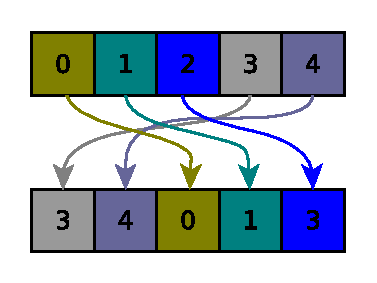
\includegraphics{sources/min_rotated_array/images/arrayrotation}
	\caption{Example of array rotation where every element if moved to the right of 2 positions. Notice how elements at position $3$ and $4$ are wrapped around to positions $1$ and $2$, respectively.}
	\label{fig:min_rotated_array:arrayrotation}
\end{figure}


\section{Problem statement}
\begin{exercise}
Given an array $A$ sorted in ascending order with no duplicates and rotated around a pivot, return the smallest element.

	\begin{example}
		\hfill \\
		Given the rotated array $\{3,4,5,6,1,2\}$ the function returns $1$.
	\end{example}

	\begin{example}
		\hfill \\
		Given the rotated array $\{0,2,3\}$ the function returns $0$.
	\end{example}

	\begin{example}
		\hfill \\
		Given the rotated array $\{3,2,1\}$ the function returns $1$.
	\end{example}
\end{exercise}

\section{Clarification Questions}

\begin{QandA}
	\item \begin{questionitem} \begin{question} Are all the elements unique?   \end{question} 	 
    \begin{answered}
		\textit{Yes, you can assume all the elements are unique}
	\end{answered} \end{questionitem}
	\item \begin{questionitem} \begin{question} Can the input array be empty?  \end{question} 	 
    \begin{answered}
		\textit{No, you might assume the array contains at least one element.}
	\end{answered} \end{questionitem}
\end{QandA}

\section{Discussion}
\label{min_rotated_array:sec:discussion}
What does it really mean for a sorted array to be rotated around an element? Given a sorted array $A=\{a_0, a_1, \ldots,a_{n-1}\}$ s.t. $ \forall \: 0 \leq i < n: a_i < a_{i+1}$, rotating A around the pivot element at index $p$ results in: $A_p=\{a_p, a_{p+1}, \ldots,a_{n-1}, a_0, a_1, \ldots, a_{p-1}\}$. In a nutshell all the elements are rotated in such a way that the element at index $p$ becomes the first element of the array. For instance, rotating the array $X=\{1,2,3,4,5\}$ around the element at index $2$, results in $X=\{3,4,5,1,2\}$. We would obtain the same result by applying a offset of either $-2$ or $3=5-2=(|A|-2)$ positions to each and every element of $X$. 

This way of performing rotation is quite common, to the point that there is an algorithm in the C++ STL\cite{cit::std::rotate} adopting such API.

\subsection{Brute-force}
\label{min_rotated_array:sec:bruteforce}
The brute-force solution to this problem is trivial and consists of simply looping through the array and keeping record of the smallest element encountered.
In C++ this can be implemented with a one-liner as shown in Listings \ref{list:min_rotated_array_bf} and \ref{list:min_rotated_array_bf_manual} both having $O(n)$ time $O(1)$ space complexity.

\lstinputlisting[language=c++, caption=Brute force solution using an explicit loop.,label=list:min_rotated_array_bf_manual]{sources/min_rotated_array/min_rotated_array_solution2.cpp}

\lstinputlisting[language=c++, caption=One-liner brute force solution.,label=list:min_rotated_array_bf_manual]{sources/min_rotated_array/min_rotated_array_solution2.cpp}

This approach should just be mentioned during the interview but, no time should be spent in the actual implementation of this idea, as the interviewer is assuming you know how to trivially search for the minimum in an unsorted array. He is clearly looking for a more advanced solution that takes advantage of the fact that the array is sorted (even if provided in a rotated form).
Yes, we did not use the word \textit{unsorted} unknowingly, because the interviewer is clearly looking for a more advanced solution that takes advantage of the fact that the array is sorted (even if provided in a rotated form), and the solutions presented above clearly ignore this fact and would work equally well on a random, unsorted and/or unrotated arrays.

\subsection{Logarithmic solution}
\label{min_rotated_array:sec:log}
As usual, when in a problem statement the word \textit{"sorted"} makes its appearance, the first thought that should cross our mind is \textbf{binary search}see Appendix \ref{sect:appendix:binary_search}). In this problem, we are almost forced to think about binary search as the problem does not only involve a sorted input, but it is also about searching. 

How can we use binary search to actually solve this problem, given the fact we have this weirdly sorted array? 
Firstly, notice that despite the fact that the array is not sorted in a canonical way, it still is very much sorted as there is an index $i$ of the array holding the smallest value from which we could iterate the array forward (and eventually continue from the start when we reach the end) and all we would see is a sorted sequence.

In order to be able to apply binary search effectively to a problem, we need some basic ingredients. In particular, we need to be able to:
\begin{enumerate}
	\item keep track of a range of elements that are currently under examination. Binary search works by cutting off parts of a search range until it becomes empty or a solution is found.  Usually such range is initialized to be the closed interval: $[l=0, r=A.size()-1]$ i.e. the entire array;
	\item analyze the element in the middle of this range;
	\item if the middle element is the one we are looking for we are done;
	\item otherwise, the search proceeds either to the left or to the right or the range. 
\end{enumerate}

The core challenges of this problem lie at steps $2$ and $4$ because we need to be able:
\begin{itemize}
	\item test whether an element is the minimum or not ($2$)
	\item decide how to split the space range into two and whether proceed with the search on the right-hand or on the left-hand side ($4$).
\end{itemize}

\subsubsection{Test if an element is the minimum}

In order to decide whether an element $a_k$ at index $k$ is the minimum, it is useful to look at one property that differentiates it from all the other values in the collection.
The minimum element is the only element s.t. both the elements on its right and left are \textbf{greater} than it (sometimes this element is referred to as an inflection point). 
Another useful property that can be helpful in the identification of the minimum is that the element on its left is always the maximum element of the array (see examples (see examples in the Section \ref{min_rotated_array:sec:discussion} and Figure \ref{fig:min_rotated_array:test_element}).
Thus, whenever $a_{k-1} > a_{k}$ (meaning that $a_k$ is the minimum and $a_{k+1}$ the maximum) or $a_{k} > a_{k+1}$ (meaning that $a_k$ is the maximum element and $a_{k+1}$ the minimum) we can stop and return because we have found the answer.

\begin{figure}
	\centering
	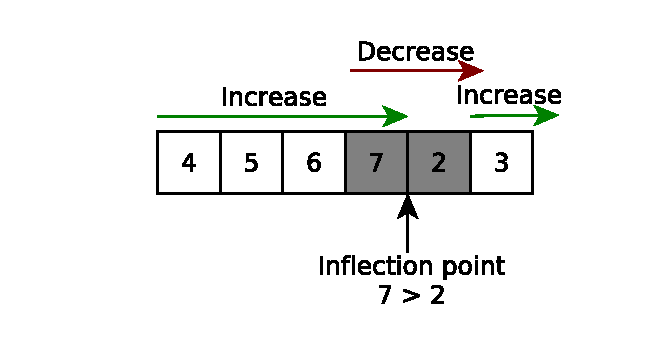
\includegraphics{sources/min_rotated_array/images/inflection_point}
	\caption{Inflection point in a rotated sorted array. When the binary search examines both element $7$ and $2$ it is able to determine the inflection point (element $2$). }
	\label{fig:min_rotated_array:test_element}
\end{figure}

In short, Listing \ref{list:test_answer} shows the condition that can be used in the binary search to test whether $a_k$ is the answer to the problem. Please note how the modulo operation is used in order to avoid having to specialize this test for the elements at the beginning and at the end of the array (positions $0$ and $A.size()-1$, respectively)..

\begin{lstlisting}[language=c++, caption={Test to verify whether the binary search can stop because an answer has been found.},label=list:test_answer]]{
	const int curr = A[k];

	const int prec = A[(k-1+A.size()) 	//+A.size() due to negative modulo
	const int succ = A[(k+1)%A.size()];
	if( (curr <= prec ) || (curr >= succ))
		return min({prec , curr , succ});
}
\end{lstlisting}

\subsubsection{Binary search range split}

The last part of the algorithm yet to be figured out is how and in which split of the array to continue the binary search if the element in the middle of the range is not good to determine the answer. An useful property of the sorted rotated array is that, when the smallest element is at position $i$ then \textbf{all the elements on its right side are smaller than the very first element of the array} (at index $0$) i.e. the following is always true:

\begin{itemize}
	\item $	(a_i < a_0) \: \wedge (a_{i+1} < a_0) \: \wedge \ldots (a_{n-1} < a_0) $
	\item $	(a_{i-1} \geq a_0) \: \wedge \: (a_{i-2} \geq a_0) \: \wedge \: \ldots \: (a_{0} \geq a_0) $
\end{itemize}
For instance, consider the sorted rotated array $\{8,9,10,5,6,7\}$: the minimum element $5$ is at index $3$ and all the elements located between index $3$ and $5$ are strictly smaller than the first element $8$ while all the elements to the left of $5$ are larger or equal than $8$.

This is the last piece of information that is needed in order to make the binary search work because we can use it to determine which portion of the two subarrays (the one to the left or to the right of \textit{middle}) to discard. Therefore, given an element at position $i$ that is not the answer, we will continue the binary search on the subarray to the left of $i$ if $a_i > a_0$, otherwise we will use the right side.

By being able to test whether an element is the smallest element in the array, and if not, how to split the array and continue the binary search, we have all the ingredients necessary to solve this problem efficiently.

An implementation of this idea is shown in the Listing \ref{list:min_rotated_array_log}.
\lstinputlisting[language=c++, caption={Logarithmic solution implemented using a standard iterative binary search.},label=list:min_rotated_array_log]{sources/min_rotated_array/min_rotated_array_solution3.cpp}


This solution as a complexity of $O(log(n))$ time and $O(1)$ space.
The code is just a straightforward implementation of the binary search where \inline{l} and \inline{r} determine the range under examination, \inline{middle} is the element in the middle of \inline{l} and \inline{r} while \inline{prec} and \inline{succ} are the element preceding and succeeding \inline{mid}, respectively. Notice how the modulo operation is used to make sure that both \inline{prec} and \inline{succ} always point to a valid element. 

%!TEX root = ../main.tex
%%%%%%%%%%%%%%%%%%%%%%%%%%%%%%%%%%
% Links:
%
% Difficulty:
% Companies: 
%%%%%%%%%%%%%%%%%%%%%%%%%%%%%%%%%%

\chapter{Search in sorted and rotated array}
\label{ch:search_sorted_rotated_array}
\section*{Introduction}
The problem presented in this chapter is another classic that often appears during interviews and that can be considered to be an evolution of the problem of finding the minimum element in a sorted and rotated array which was covered in Chapter \ref{ch:min_rotated_array} (at page \pageref{ch:min_rotated_array}).
The two problems are so deeply linked that it is actually possible to solve this problem by using the other's solution structure. 

\section{Problem statement}
\begin{exercise}
Write a function that given an ascending sorted array $A$ of lenght $n$ with no duplicates and rotated around a pivot $p$ (meaning that the array has been rotated such that the smallest element of $A$ ends up at index $p$), and an integer $t$, returns:
\begin{itemize}
	\item if $t$ does not exists in $A$ it returns $-1$ 
	\item otherwise the index of $A$ where $t$ appears.
\end{itemize}


	\begin{example}
		\hfill \\
		Given $A=\{3,4,5,6,1,2\}$ and $t=5$ the function returns $2$.
		
	\end{example}

	\begin{example}
		\hfill \\
		Given $A=\{3,4,5,6,1,2\}$ and $t=7$ the function returns $-1$.
		
	\end{example}
\end{exercise}

\section{Clarification Questions}

\begin{QandA}
	\item \begin{questionitem} \begin{question} Are all the elements unique?   \end{question} 	 
    \begin{answered}
		\textit{Yes, you can assume all the elements are unique}
	\end{answered} \end{questionitem}
	\item \begin{questionitem} \begin{question} Can the input array be empty?  \end{question} 	 
    \begin{answered}
		\textit{No, you might assume the array contains at least one element.}
	\end{answered} \end{questionitem}
\end{QandA}


\section{Discussion}
\label{search_sorted_rotated_array:sec:discussion}


\subsection{Brute-force}
\label{search_sorted_rotated_array:sec:bruteforce}
As was the case for the problem of finding the minimum in a sorted and rotated array (Chapter \ref{ch:min_rotated_array}) the brute-force solution to this current problem is trivial and consists of simply running a linear search in the entire array as shown in Listing \ref{list:search_sorted_rotated_array:bruteforce}.
Not surprisingly, the complexity of this implementation is linear in time and constant in space.

\lstinputlisting[language=c++, caption={Brute force solution (linear search) to the problem of finding an element in a sorted and potentially rotated array.},label=list:search_sorted_rotated_array:bruteforce]{sources/search_sorted_rotated_array/search_sorted_rotated_array_solution1.cpp}

\subsection{Logarithmic time solution}
\label{search_sorted_rotated_array:sec:log}
The solution presented in Section \ref{search_sorted_rotated_array:sec:bruteforce} above is far from optimal given we can solve this problem in logarithmic time and constant space (as we did for the problem in Chapter \ref{ch:min_rotated_array}).

The main point is that we need to take advantage of the fact that the array is sorted and that, if we know the pivot location, $p$ then we can logically divide the array into two subarrays, starting and ending at indices:
\begin{enumerate}
	\item $0$ and $p-1$
	\item $p$ and $n-1$ ($n$ is the size of the array)
\end{enumerate}
Both arrays are sorted and thus binary search can be applied in each of the subarrays separately. This is why we can reuse the solution to the problem of finding the minimum element in a sorted and rotated array to solve this one.

To summarize the algorithm, proceed as follows:
\begin{itemize}
	\item search for the pivot index $p$
	\item search for $t$ in $A[0,p-1]$. If the search is successful return the found index for $t$.
	\item search for $t$ in $A[p,n-1]$.  If the search is successful return the found index for $t$.
	\item None of the searches had success. $t$ is not in the array. Return $-1$.
\end{itemize}

This algorithm can be implemented as shown in Listing \ref{list:search_sorted_rotated_array:log}. Note that the function \inline{find_idx_min} is almost identical to the one in Listing \ref{list:min_rotated_array_log} and has been modified so as to return the index instead of the value for the smallest element in the array.

Also note that the function \inline{midpoint} is not implemented as \inline{(l+r)/2} because that might cause overflow during the computation of \inline{(l+r)} even if the final result fits in a \inline{int}. Specifically, it fails if the sum of low and high is greater than the maximum positive \inline{int} value ($2^{31} - 1$ in most C++ implementation). The sum overflows to a negative value and the value stays negative when divided by two. In C++ this causes an array index out of bounds with unpredictable results. In Java, it throws \inline{ArrayIndexOutOfBoundsException}.

Finally, the function \inline{binary_search} implements a simple and canonical recursive binary search. 
The complexity of the overall implementation is $O(log(n))$ in time and $O(1)$ in space.

\lstinputlisting[language=c++, caption={Log time solution (using binary search) to the problem of finding an element in a sorted and rotated array.},label=list:search_sorted_rotated_array:log]{sources/search_sorted_rotated_array/search_sorted_rotated_array_solution2.cpp}

%!TEX root = ../main.tex
%%%%%%%%%%%%%%%%%%%%%%%%%%%%%%%%%%
% Links:
%
% Difficulty:
% Companies: 
%%%%%%%%%%%%%%%%%%%%%%%%%%%%%%%%%%

\chapter{Verify BST property}
\label{ch:verify_BST}
\section*{Introduction}
This problem is binary search trees, which are one of the most discussed data structures during coding interviews. This problem has been asked at \textbf{Microsoft, Google, Amazon, Ebay} and it is among the group of questions that should be well understood and digested because its solution's structure can be applied to many others on binary trees.

\section{Problem statement}
\begin{exercise}
Given a binary tree \cite{cit:wiki:BST}, determine if it is a valid binary search tree.

Assume a BST is defined as follows:
\begin{itemize}
    \item The left subtree of a node contains only nodes with keys less than the node's key.
    \item The right subtree of a node contains only nodes with keys greater than the node's key.
\end{itemize}
You can assume that the tree structure is defined as shown in Listing \ref{list:verify_BST:tree_structure}: 

\end{exercise}

\begin{lstlisting}[language=c++, caption=Binary tree definition used in this exercice.,label=list:verify_BST:tree_structure]

 struct TreeNode {
     int val;
     TreeNode *left;
     TreeNode *right;
     TreeNode(int x) : val(x), left(nullptr), right(nullptr) {}
 };
 \end{lstlisting}


\begin{example}
	\hfill \\
	For the following tree the function should return \textbf{false}.
	\begin{verbatim}
	    5
	   / \
	  1   4
	     / \
	    3   6
	\end{verbatim}
\end{example}

\begin{example}
	\hfill \\
	For the following tree the function should return \textbf{true}.
	\begin{verbatim}
	    2
	   / \
	  1   3
	\end{verbatim}
	
\end{example}

\begin{example}
\label{example:verify_BST_:one}
	\hfill \\
	For the following tree the function should return \textbf{true}.
	\begin{verbatim}
	    10
	   / \
	  1   14
	 / \    \
0  9     16
        /  \
       15   19
	\end{verbatim}
	
\end{example}


\section{Clarification Questions}

\begin{QandA}
	\item Are all elements in the tree distinct?
	\begin{answered}
		\textit{Yes, you can assume all elemets are distinct.}
	\end{answered}
	\item How many nodes does the tree contain?
	\begin{answered}
		\textit{Up to $10^6$ nodes.}
	\end{answered}
\end{QandA}

\section{Discussion}
\label{verify_BST:sec:discussion}
The question is asking for a function that verifies whether a given tree is a binary search tree or not. But what does it mean exactly?
A tree $T$ is a binary search tree if:
\begin{enumerate}
	\item Every node has two subtree (named left and right, respectively) i.e. $T$ is a binary tree
	\item given a node $n$ in the tree \textbf{all} the nodes in its left subtree are smaller than the value in $n$.
	\item additionally,  \textbf{all} nodes in the right subtree are larger.
\end{enumerate}
For instance the tree in the example \ref{ex:verify_BST:no_BST} is not a valid BST because node $15$ is a right descendent of the root but is it not greater than it. 
\begin{lstlisting}[language=c++,frame=single,caption={Binary tree, but not a binary search tree.}",label=ex:verify_BST:no_BST, numbers=none]
	    20
	    / \
	   10 30
	     / \
	    15  40
\end{lstlisting}


\subsection{A common mistake}
When solving this question a very common mistake is to use the following greedy algorithm to verify the BST property: for each node $n$ of the tree verify that \lstinline[columns=fixed]{n.val > n->left.val && n.val < n->right.val} i.e. that the value of the node curreclty analyzed is greater than the value of its left child but smaller than its right one. This algorithm might work even for some trees but fails on others, and it is thus not correct. For instance the algorithm described above fails on the example \ref{ex:verify_BST:no_BST} as it will say that it is a valid BST.

It is clear at this point that all nodes in the tree need to be visited in order to verify whether the BST property holds and that somehow the information about the values from nodes higher in the tree need to be passed down to the children and descendants. Let's see how this can be done.

\subsection{Top Down approach}
\label{verify_BST:sec:topdown}
When talking about tree, one should immediately think about a top down approach and recursion. This problem is no different and in-fact  becomes almost trivial if approached using recursione and the following key considerations are made:
\begin{enumerate}
	\item every node can be thought as the root of a tree for which the BST property needs to hold (and thus verified). 
	\item empty trees satisfy the BST property
	\item every nodes must be within a certain range that is determined by its parent. For instance, given the node $15$ in the example \ref{example:verify_BST_:one}, in order for the tree to be a valid it must be within the range $(14,16)$. Why is that? Because its parent, the node $16$ must be within the range $(14,+\infty)$ and additionally node $15$, being the left subtree of node $16$ must be lower than its parent. The same reasoning can be applied recusively up to the root of the tree where the range of the value is simply $(-\infty, +\infty)$ (no constraints). 

	The node $9$ in the example \ref{example:verify_BST_:one} must be within the range $(1,10)$ for similar reasons.
\end{enumerate}


To summarize, we can visit the tree in a top-down fashion and maintain a range that the current node must satisfy starting with a range equal to $(-\infty, +\infty)$ for the root (meaning that de-facto there is no restriction on the value the root can take). Once the value is checked against the range, then the same function can be applied to the right and left children but making sure that the range is modified accordingly when recurring on the children. 

But how does such a range change when visiting down the tree? The idea is simple: Given a node $n$ with parent $p$ and range \( (l_p, u_p) \) then:
\begin{itemize}
	\item if $n$ is the right child of $p$, then the range for $n$ is: $(p, u_p)$: all nodes in the right subtree of $p$ must be \textbf{higher} than $p$. Note that $p > l_p$ (otherwise the BST property would be violeted when checking $p$) and thus the range for $n$ becomes smaller meaning that all the constrains coming from the ancestors of $p$ will also be satisfied with the new range $(p, u_p)$.
	\item A similar reasoning applies if $n$ is the left child of $p$. The range for $n$ is then : $(l_u,p)$.
\end{itemize}

The idea above is shown in Listing \ref{list:verify_BST}. Note how short and concise the code can be implemented with recursion.  The complexity of this approach is $O(n)$ time and $O(1)$ space (if you do not count the space on the stack taken by the recursion.
\lstinputlisting[language=c++, caption=Linear time recursive solution to the problem of verifying the BST property.,label=list:verify_BST]{/home/dspataro/git/algorithm_articles/sources/verify_BST/verify_BST_solution1.cpp}


\subsection{Brute force}
Another way to solve this problem is to read carefully the definition of BST and realize that, for each node $n$ we need to check if the left subtree contains any element greater than $n$ and whether its right subtree contains any element smaller than $n$. This problem becomes almost trivial provided two functions are available, \lstinline[columns=fixed]{min_tree(TreeNode* root)} and \lstinline[columns=fixed]{max_tree(TreeNode* root)} for retrieving the min and max value respectively of a tree. The idea above can be implemented as shown in Listing \ref{list:verify_BST_bruteforce}

\lstinputlisting[language=c++, caption=Quadratic solution to the problem of verifying the BST property.,label=list:verify_BST_rbuteforce]{/home/dspataro/git/algorithm_articles/sources/verify_BST/verify_BST_solution2.cpp}
%!TEX root = ../main.tex
%%%%%%%%%%%%%%%%%%%%%%%%%%%%%%%%%%
% Links:
%
% Difficulty:
% Companies: 
%%%%%%%%%%%%%%%%%%%%%%%%%%%%%%%%%%

\chapter{Clone a linked list with random pointer}
\label{ch:clone_list_random_pointer}
\section*{Introduction}
This section discusses a very cool and interesting problem on linked list. The linked list we are dealing with here is a singly linked one, with an additional pointer that \textbf{might} point to another node in the list. The C++ definition of said list is given in Listing \ref{list:clone_list_random_pointer:list_definition}. Please note the additional field \lstinline[columns=fixed]{random} which differentiates it from other linked list definitions seen in other chapters (See Capter \ref{ch:delete_duplicates_list} and Listing \ref{list:delete_duplicates_list:linked_list}).

\begin{lstlisting}[language=c++, caption={Definition of a linked list with a random pointer.},label=list:delete_duplicates_list:linked_list]

template <class T> 
class Node
{
    public:
  T val;
  Node *next;
  Node *random;

  Node(const T &_val)
  {
    val    = _val;
    next   = nullptr;
    random = nullptr;
  }
};
\end{lstlisting}

\section{Problem statement}
\begin{exercise}
Given a linked list of the type defined in Listing \ref{list:clone_list_random_pointer:list_definition} return a deep-copy of it.
\end{exercise}

In this chapter we will be representing graphically a list using a list of pairs of integers. Each pair $(v,r)$ represent a node of the list where:
\begin{itemize}
	\item[-] $v$ is the payload of the node
	\item[-] $r$ is the index of the node that the random pointer points to. $-1$ represents \lstinline[columns=fixed]{nullptr}.
\end{itemize} 
For instance the list: $[(7,-1),(13,0),(11,4),(10,2),(1,0)]$ represent the list shown in Figure \ref{fig:clone_list_random_pointer:list1}.

\begin{figure}
	\label{fig:clone_list_random_pointer:list1}
	\centering
	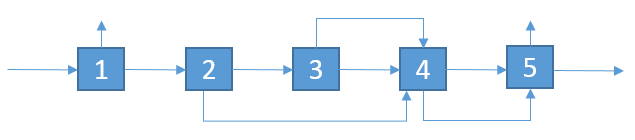
\includegraphics[scale=0.6]{/home/dspataro/git/algorithm_articles/sources/clone_list_random_pointer/images/random_list_1}
	\caption{Linked list wit random pointer.}
\end{figure}


\section{Clarification Questions}
The problem is clearly aimed at testing the list manipulation and it is not really about algorithm design. So question related to the size of the input do not help much. Instead it is better to ask question related to the structure of the list itself to see if there is any pattern in the lists we can take advantage of.
\begin{QandA}
	\item Is it guaranteed that at least one not-null random pointer exists?
	\begin{answered}
		\textit{No, all random pointer might be null.}
	\end{answered}
	\item Can a random pointer point to itself?
	\begin{answered}
		\textit{Yes, you can have a node pointing to itself.}
	\end{answered}
	
\end{QandA}

\section{Discussion}
\label{clone_list_random_pointer:sec:discussion}
The two solutions presented in this chapter are fundamentally different and comes with asymptotic performances differences in memory.
The solution presented in Section \ref{clone_list_random_pointer:sec:bruteforce} uses additional memory (linear amount) while the second one works in constant time but it is harder to digest and to come up with in the first place.

\subsection{Linear memory solution}
\label{clone_list_random_pointer:sec:bruteforce}
The solution presented in this section can be split into a number of distinct steps:
\begin{enumerate}
	\item Create a copy of the list with all the  next and random pointers set to \lstinline[columns=fixed]{nullptr}. Save all the pointers in an \lstinline[columns=fixed]{std::vector<Node<T>*> ptrs;}.
	\item For each node in the input list, while traversing it, save in a \lstinline[columns=fixed]{map<Node<T>*, int> P} the index of that node in the list. We want to remember for each pointer the index where it appears in the original input list. 
	\item Fix the next pointers of all nodes s.t. \lstinline[columns=fixed]{ptrs[i]->next} points to  \lstinline[columns=fixed]{ptrs[i+1]}. At this point we have a new singly linked list with broken random pointers. Basically an half cloned list.
	\item At this point we can traverse the original list once again, and if the current node $c$ has a not-null random pointer $c->p$ we can query $P$ to see which index \lstinline[columns=fixed]{P[c->p]} has in the input. We know then that we need connect also the corresponding element of $c$ in the copy with the node of index \lstinline[columns=fixed]{P[c->p]} in the copy.
\end{enumerate}

The idea above can be implemented as shown in the Listing \ref{list:clone_list_random_pointer_1}


\lstinputlisting[language=c++, caption={Linear Memory solution to the problem of copying a linked list with random pointers.},label=list:clone_list_random_pointer_1]{/home/dspataro/git/algorithm_articles/sources/clone_list_random_pointer/clone_list_random_pointer_solution1.cpp}

This approach has a complexity of $O(n)$ for both time and space. The time complexity is already optimal as we cannot do better than linear time, considering that to do a copy we need to look at all the nodes at least once. The space complexity can be improved though, and as we will see in Section \ref{clone_list_random_pointer:sec:interleaved_lists} it can be brought down to constant.

\subsection{Constant memory solution}
\label{clone_list_random_pointer:sec:interleaved_lists}
\subsubsection{Copy interleaved with the original list}
The idea behind the solution presented in this section is to construct the copy such that its nodes are interleaved with the ones from the original list. For instance given the input list\footnote{Remember that $(x,-1)$ is a node containing the value $x$ and with random pointer set to \lstinline[columns=fixed]{nullptr}}: $A = [(7,-1),(13,0),(11,4),(10,2),(1,0)]$ we want to have an interleaved list that look like the following: $A' = [(7,-1),(7,-1),(13,0),(13,-1),(11,4),,(11,-1),(10,2),(10,-1),(1,0),(1,0)]$ (see Figure \ref{fig:clone_list_random_pointer:interleaved}) where every node at even indexes is a copy of its predecessor with a random pointer set to \lstinline[columns=fixed]{nullptr}.  See function \lstinline[columns=fixed]{fix_random_pointers} in Listing \ref{list:clone_list_random_pointer_2}.


\begin{figure}
	\label{fig:clone_list_random_pointer:interleaved}
	\centering
	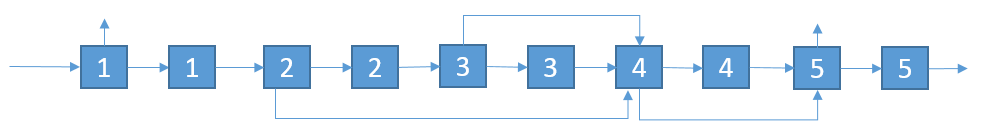
\includegraphics[scale=0.5]{/home/dspataro/git/algorithm_articles/sources/clone_list_random_pointer/images/random_list_2}
	\caption{Intermediate interleaved list.}
\end{figure}


In more abstract terms given:
\begin{itemize}
	\item[-] the input list  $A= a_0 \rightarrow a_1 \rightarrow \ldots \rightarrow a{n-1}$
	\item[-] a copy of A  $B = b_0 \rightarrow b_1 \rightarrow \ldots \rightarrow b{n-1}$ 
\end{itemize}

\subsubsection{Fix the random pointers in the interleaved list}
Then we want to get a list $I$ of size $2n$: $I=a_0 \rightarrow b_0 \rightarrow a_1 \rightarrow b_1 \rightarrow a_2 \rightarrow b_2 \rightarrow \ldots \rightarrow a_{n-1} \rightarrow b_{n-1}$. Having the two lists arranged this ways is quite useful because we can still visit the original lists and at the same time operate on its mirror one by simply modifying the nodes at odd indexes. An interleaved list has a even number of nodes. All the ones at even positions $(0,2,\ldots)$ belong to the original lists while all the nodes with odd indexes $(1,3,\ldots)$ to the copy. Given a node $n_{2k}=(x,r)$ at an even index $2k$, we can fix the random pointer for the clone of this node $n_{2k+1}=(x,-1)$ at index $2k+1$ by simply fixing its random pointer to the value pointed by $n_{2k}$\lstinline[columns=fixed]{->random->next}. See Figure \ref{fig:clone_list_random_pointer:interleaved_fixed} where the red lines represent the mirrored for the random pointers in the original list and function \lstinline[columns=fixed]{split_fix_random_pointers} in Listing \ref{list:clone_list_random_pointer_2}.

\begin{figure}
	\label{fig:clone_list_random_pointer:interleaved_fixed}
	\centering
	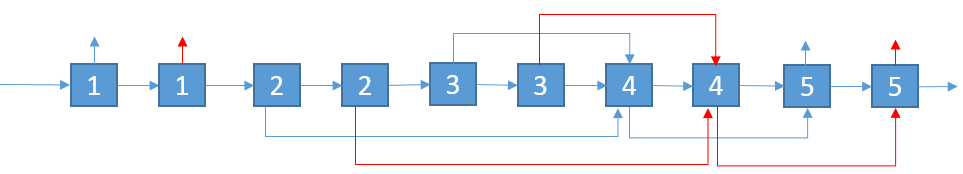
\includegraphics[scale=0.5]{/home/dspataro/git/algorithm_articles/sources/clone_list_random_pointer/images/random_list_3}
	\caption{Interleaved list with fixed random pointers.}
\end{figure}

\subsubsection{Extract the cloned list}
Once we reach this point we have basically two copies of the original list (with random pointers fixed) interleaved with each other. All is it necessary at this point is pull out the cloned list from the interleaved one. This is easily achievable as all we need to do is to remove all the odd nodes, and in the process connect all together (see function \lstinline[columns=fixed]{split_list} in Listing \ref{list:clone_list_random_pointer_2}).


\lstinputlisting[language=c++, caption={Constant memory solution to the problem of copying a linked list with random pointers using an interleaved list.},label=list:clone_list_random_pointer_2]{/home/dspataro/git/algorithm_articles/sources/clone_list_random_pointer/clone_list_random_pointer_solution2.cpp}
%!TEX root = ../main.tex
%%%%%%%%%%%%%%%%%%%%%%%%%%%%%%%%%%
% Links:
%
% Difficulty:
% Companies: 
%%%%%%%%%%%%%%%%%%%%%%%%%%%%%%%%%%

\chapter{Delete duplicates from Linked List}
\label{ch:delete_duplicates_list}
\section*{Introduction}
The problem presented in this chapter is an easy one on Linked list that has been asked to preliminary interview steps many times already. It is therefore very important that this problem is understood well and you can implement it quickly and most importantly flawlessly during an interview. 
\section{Problem statement}
\begin{exercise}
Given a singly linked link $L$ (see definition at Listing \ref{list:delete_duplicates_list:linked_list}), return a linked list with no duplicated.
\end{exercise}
\begin{lstlisting}[language=c++, caption=Singly Linked list definition,label=list:delete_duplicates_list:linked_list]
template<typename T>
struct Node {
    T val;
    Node *next;
    Node(T x) : val(x), next(nullptr) {}
};
\end{lstlisting}

\begin{example}
	\hfill \\
	\begin{itemize}
		\item[-] Input: $1 \rightarrow 1 \rightarrow 2$
		\item[-] Output: $1 \rightarrow 2$
	\end{itemize}
\end{example}

\begin{example}
	\hfill \\
	\begin{itemize}
		\item[-] Input: $1 \rightarrow  2 \rightarrow  2 \rightarrow  2 \rightarrow  2 \rightarrow  3 \rightarrow  4 \rightarrow  4 $
		\item[-] Output: $1 \rightarrow  2 \rightarrow 3 \rightarrow  4$
	\end{itemize}
\end{example}

\section{Clarification Questions}

\begin{QandA}
	\item Can the input list be modified?
	\begin{answered}
		\textit{Yes.}
	\end{answered}
	
\end{QandA}

\section{Discussion}
\label{delete_duplicates_list:sec:discussion}
As you can imagine there are many approaches that can be adopted in order to solve this problem, but we will focus on basically two, with the second being a refinement of the first which will lead to an elegant yet efficient solution.

\subsection{Brute-force}
\label{delete_duplicates_list:sec:bruteforce}
The easiest solution possible consist in:
\begin{enumerate}
	\item Create a vector that basically contains a copy of the list
	\item Remove duplicates from the vector
	\item Create a new List with the content of the duplicate free vector
\end{enumerate}
This solution is straightforward but as you can imagine not optimal. A possible implementation is shown in Listing \ref{list:delete_duplicates_list_brite_force1} where for the step $2$ the  remove-erase idiom\cite{cit::wiki::remove-erase} is used to remove duplicates from the vector(the erase part is actually not necessary in this case).

\lstinputlisting[language=c++, caption={C++ solution $O(n)$ time and $O(n)$ space solution to the problem of removing duplicates from a Linked List using std::remove.},label=list:delete_duplicates_list_brite_force1]{sources/delete_duplicates_list/delete_duplicates_list_solution1.cpp}

This solution is optimal in time but we are not taking advantage of the fact that the we can modify the list in place and it is not necessary to create a brand new List to be returned. 

\subsection{In-place $O(1)$ space solution}
\label{delete_duplicates_list:sec:linear_space}
In the solution describe in Section \ref{delete_duplicates_list:sec:discussion} we did use of additional space to both remove the duplicates and also to avoid the pain of rearranging the input list by creating a brand new list containing no duplicates. It is possible though with a bit of thinking to write a in-place solution that uses no additional space. 

The main idea is that since the list is \textbf{sorted}, duplicate element will be one after the other, and we can take advantage of this fact by simply ignoring pair of consecutive nodes that have the same payload. Ignored nodes can therefore be deleted. The only complications is that we need to make sure to connect the first occurrence of every Node in the list with each other For this reason we need to therefore remember the first Node of a stride of the same value.

This idea is implemented in Listing \ref{list:delete_duplicates_list_lineartime}. Note that:

\begin{itemize}
	\item[-] The base case \lstinline[columns=fixed]{if(!head || !head->next) return head;} is making sure that if we are examining the last element of the list (or an empty list) then there is no duplicate to ignore and thus we can return this element.
	\item[-] otherwise, we are looking at a list with \textbf{at least} two elements. These two elements can be potentially the start of a stride of equal element that we want to ignore. We keep a pointer,\lstinline[columns=fixed]{Node<T>* head;} (which is never modified) to the first element  of the stride and advance a second pointer, \lstinline[columns=fixed]{Node<T>* head_n;}, until we either reach the end of the list or we find an element that is different from the first one, \lstinline[columns=fixed]{while ( head_n && head -> val == head_n -> val)}. All the advanced elements are deleted. At the end of the loop the second pointer  is pointing to either:
	\begin{itemize}
		\item[-] An element different than the element pointed by the first one. The stride of equal elements is processed and  \lstinline[columns=fixed]{head->next} can now point to the second pointer.
		\item[-] \lstinline[columns=fixed]{nullptr}. We have reached the end of the input list. We are done.
	\end{itemize}
\end{itemize}

The time and space complexity for this approach are $O(n)$ and $O(1)$, respectively. All the nodes of the list are  visited at most once.

\lstinputlisting[language=c++, caption={C++ solution $O(n)$ time and $O(1)$ space solution to the problem of removing duplicates from a Linked.},label=list:delete_duplicates_list_lineartime]{sources/delete_duplicates_list/delete_duplicates_list_solution2.cpp}


\section{Common Variations and follow-up questions}
One follow-up question that the interviewer might be keen to ask is related to the deletion of the duplicate nodes. In the Listing \ref{list:delete_duplicates_list_lineartime} we see that the nodes are deleted using the \lstinline[columns=fixed]{operator delete}, but what if the list was not allocated using \lstinline[columns=fixed]{operator new}? The question is left for the reader.

\begin{exercise}
How would the solution change if the nodes were allocated using a custom allocator? (spoiler, a custom deleter is also needed.)
\end{exercise}

%!TEX root = ../main.tex
%%%%%%%%%%%%%%%%%%%%%%%%%%%%%%%%%%
% Links:
%
% Difficulty:
% Companies: 
%%%%%%%%%%%%%%%%%%%%%%%%%%%%%%%%%%

\chapter{Generate points in circle uniformly}
\label{ch:random_points_in_circle}
\section*{Introduction}
The problem described in this Chapter is about generating a (possibly large) number of random points in a circle of a certain radius. Said points need to be generated uniformly. Despite its simplicity the problem still poses some unexpected challenges and difficulties. We will discuss how to approach this problem and also one solution that many candidates provides and that seems just correct but that should absolutely be avoided as it is not correct (spoiler it does not distribute points uniformly). We will also look at some cool figures or points in a circle.

\section{Problem statement}
\begin{exercise}
Write a function that, given a circle of radius $r$ and centered at $(x,y)$ where $r,x,y \in \mathcal{R}$ returns a uniformly distributed point in the circle.
\end{exercise}



\begin{example}
	\hfill \\

	
\end{example}

\section{Clarification Questions}

\begin{QandA}
	\item What does really mean for the point to be uniformly distributed?
	\begin{answered}
		\textit{It means that every point of the circle has the same probability of being picked/generated by the function}
	\end{answered}
\end{QandA}

\section{Discussion}
\label{random_points_in_circle:sec:discussion}

\subsubsection{Wrong approach}
\label{random_points_in_circle:sec:buggy}
Let's start by discussing a common approach that comes naturally to mind. One might think that in order to pick a point in the circle is it sufficient to 
\begin{enumerate}
	\item Pick a random angle $\theta \in [0, 2\pi[ $
	\item Pick a random radius $\overline{r} \in [0,r]$
	\item Generate the Cartesian coordinates of the point given the radius and the angle (polar coordinates \cite{cit:wiki:polar_coordinates}) as (see Figure \ref{fig:random_points_in_cirle:polar_coordinates}):
	\begin{gather*}
		 x=\overline{r}\sin(\theta) \\
		 y=\overline{r}\cos(\theta) 
	\end{gather*}
\end{enumerate}

\begin{figure}
	\label{fig:random_points_in_cirle:polar_coordinates}
	\centering
	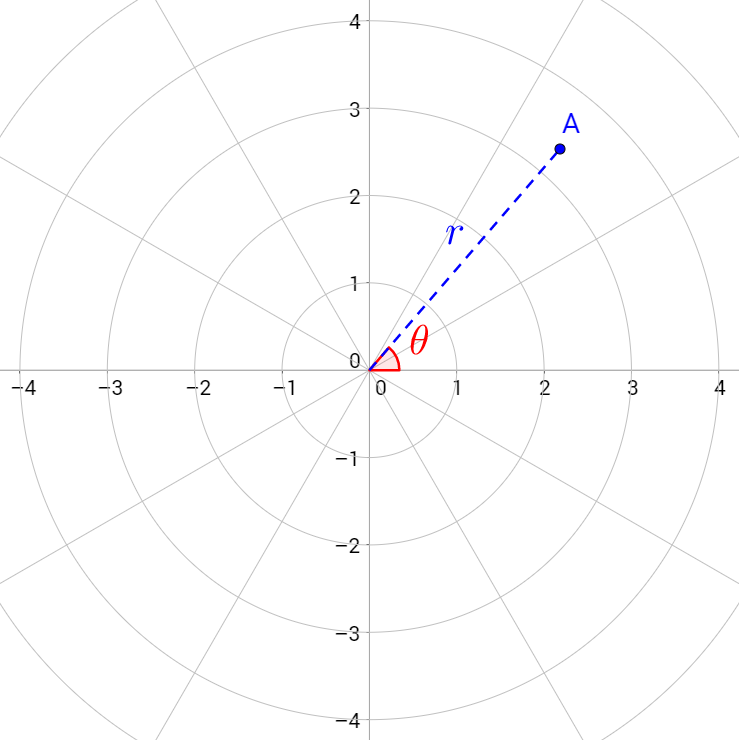
\includegraphics[scale=0.3]{sources/random_points_in_circle/images/polar-coordinate}
	\caption{Generation of a random point in polar coordinates given a random angle $\theta$ and a random radius $r$.}
\end{figure}

Despite its simplicity this approach is wrong as it does not produce points uniformly distributed in the circle? Before having a quick look at the proof it is instructive to have a look Figure \ref{fig:random_points_in_cirle:buggy} which is drawing a large number of points on the circle generated using this buggy solution. As you can see the points are not generated uniformly as their density is higher towards the center. 

\begin{figure}
	\label{fig:random_points_in_cirle:buggy}
	\centering
	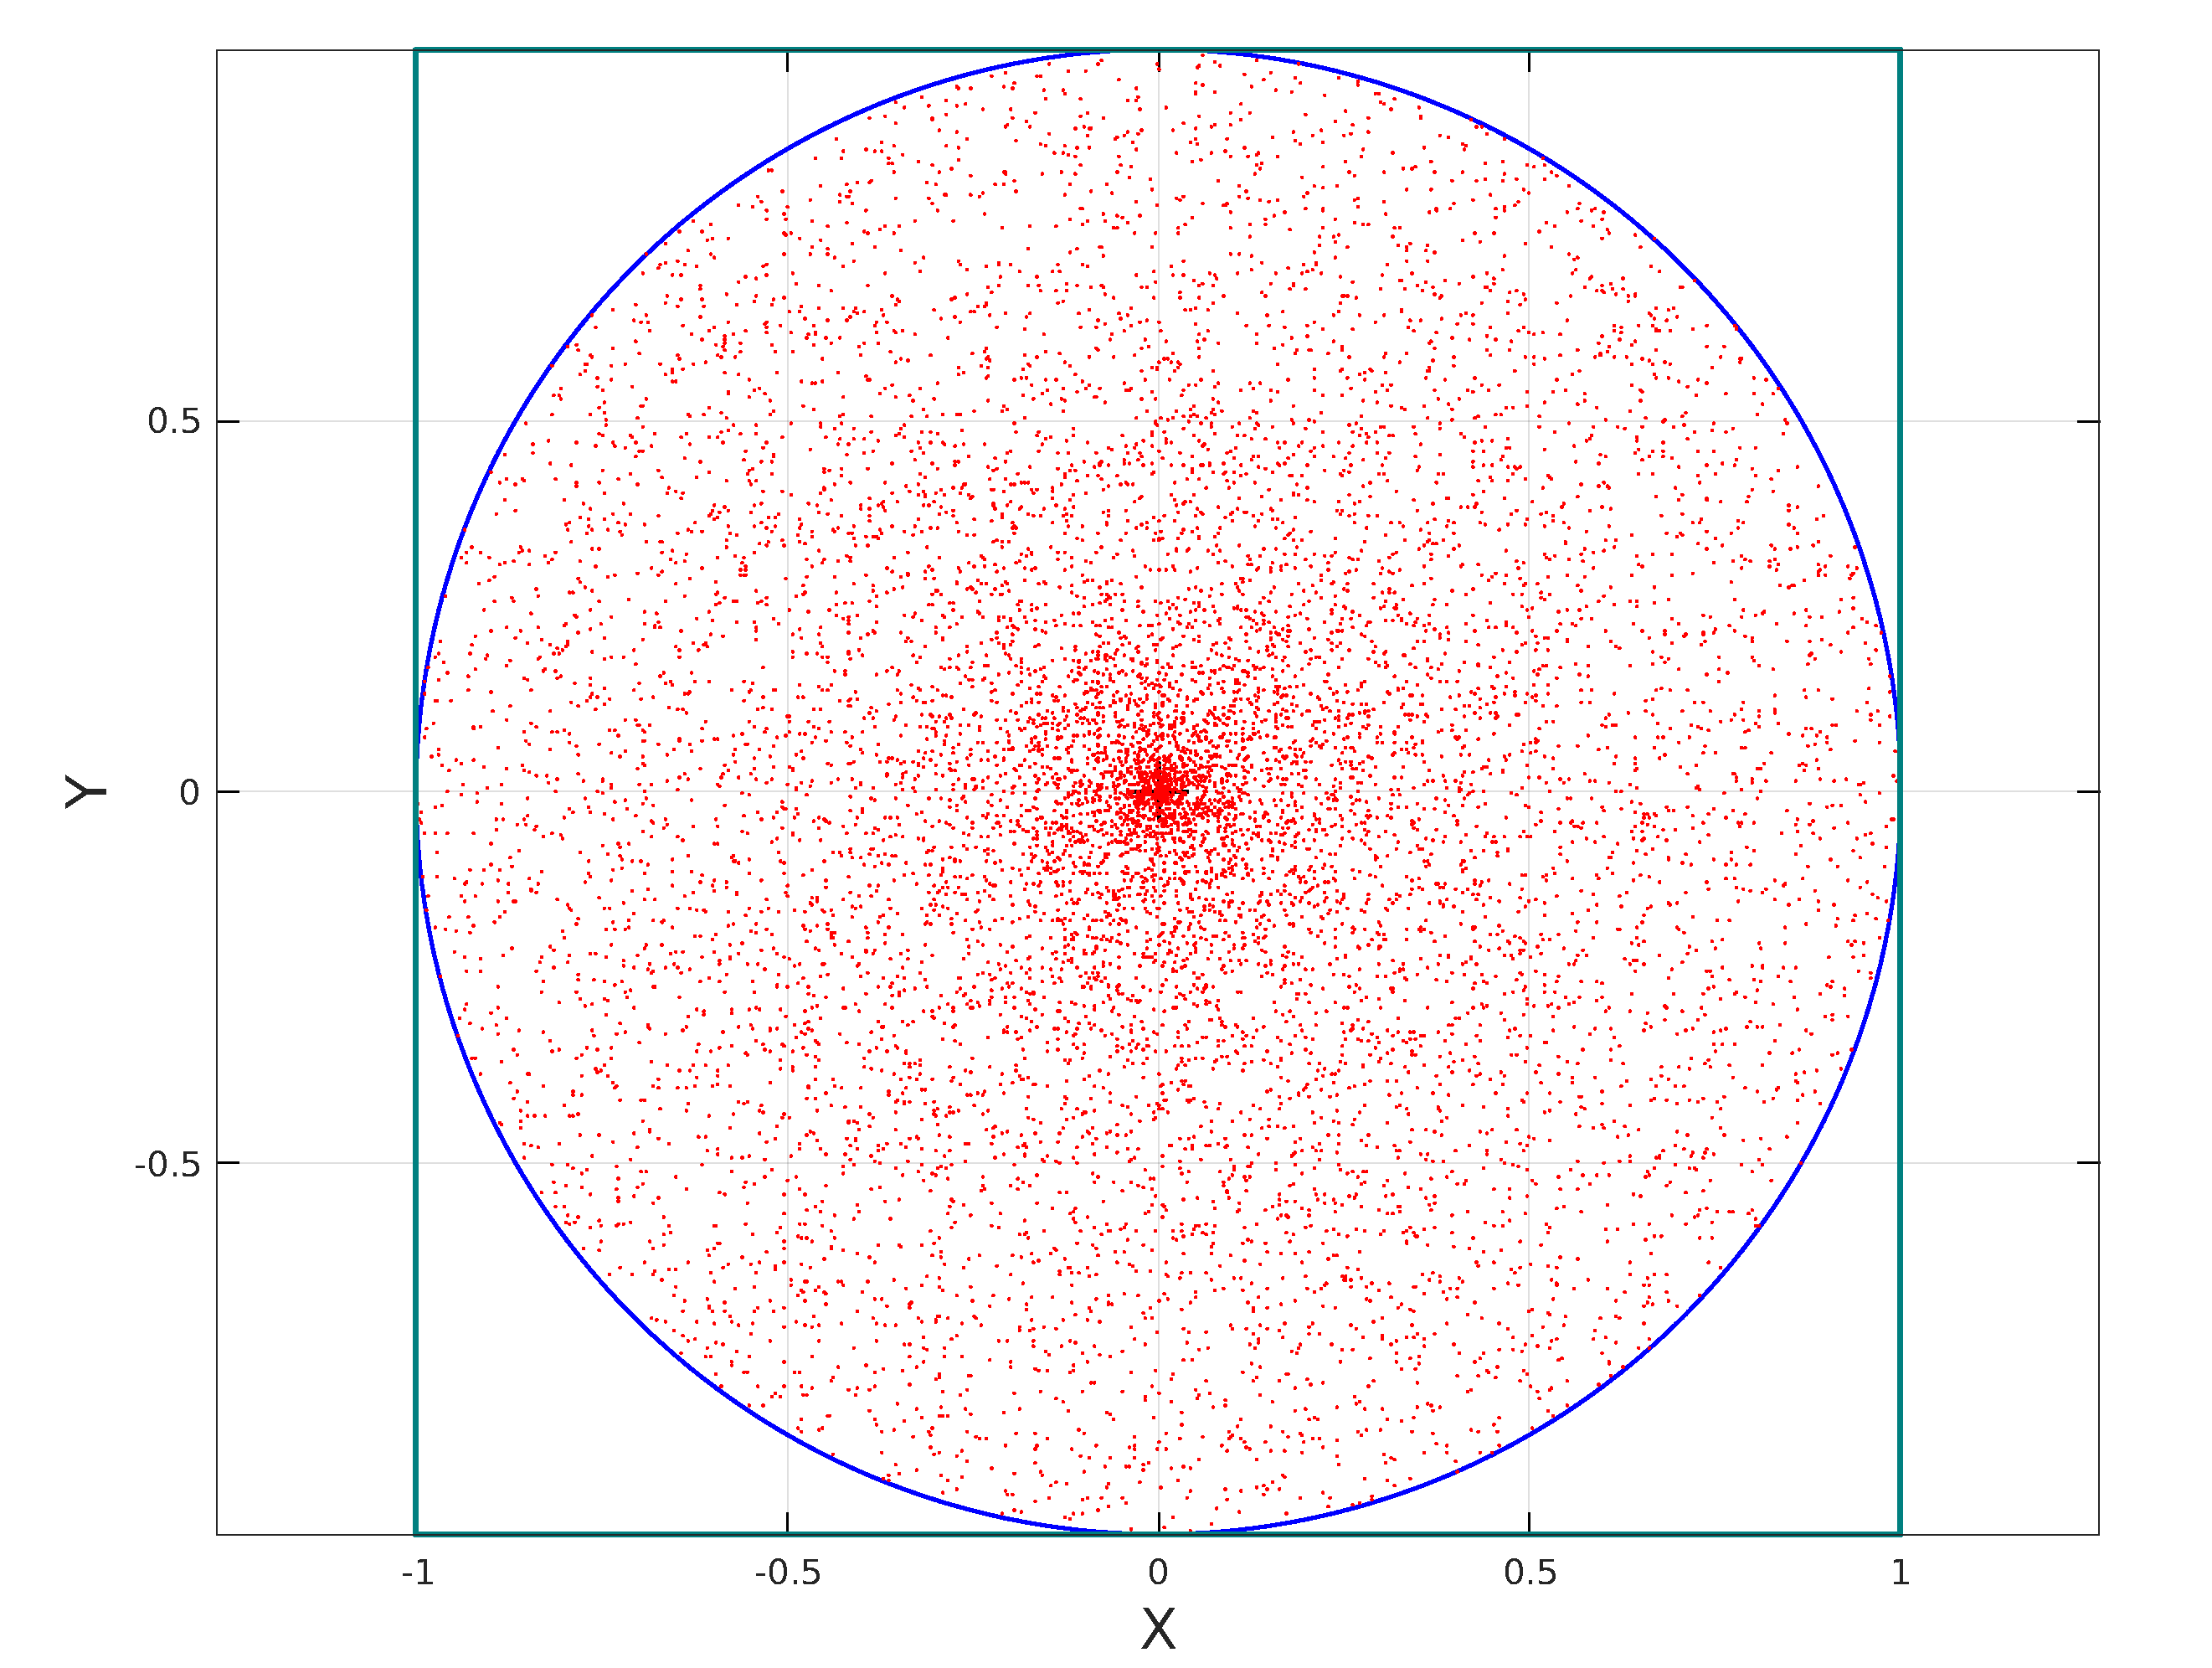
\includegraphics[scale=0.3]{sources/random_points_in_circle/images/buggy_points}
	\caption{Large number of points generated using the approach described in Section \ref{random_points_in_circle:sec:buggy}.}
\end{figure}

\subsubsection{Loop approach}
\label{random_points_in_circle:sec:loop}

\begin{figure}
	\label{fig:random_points_in_cirle:loop}
	\centering
	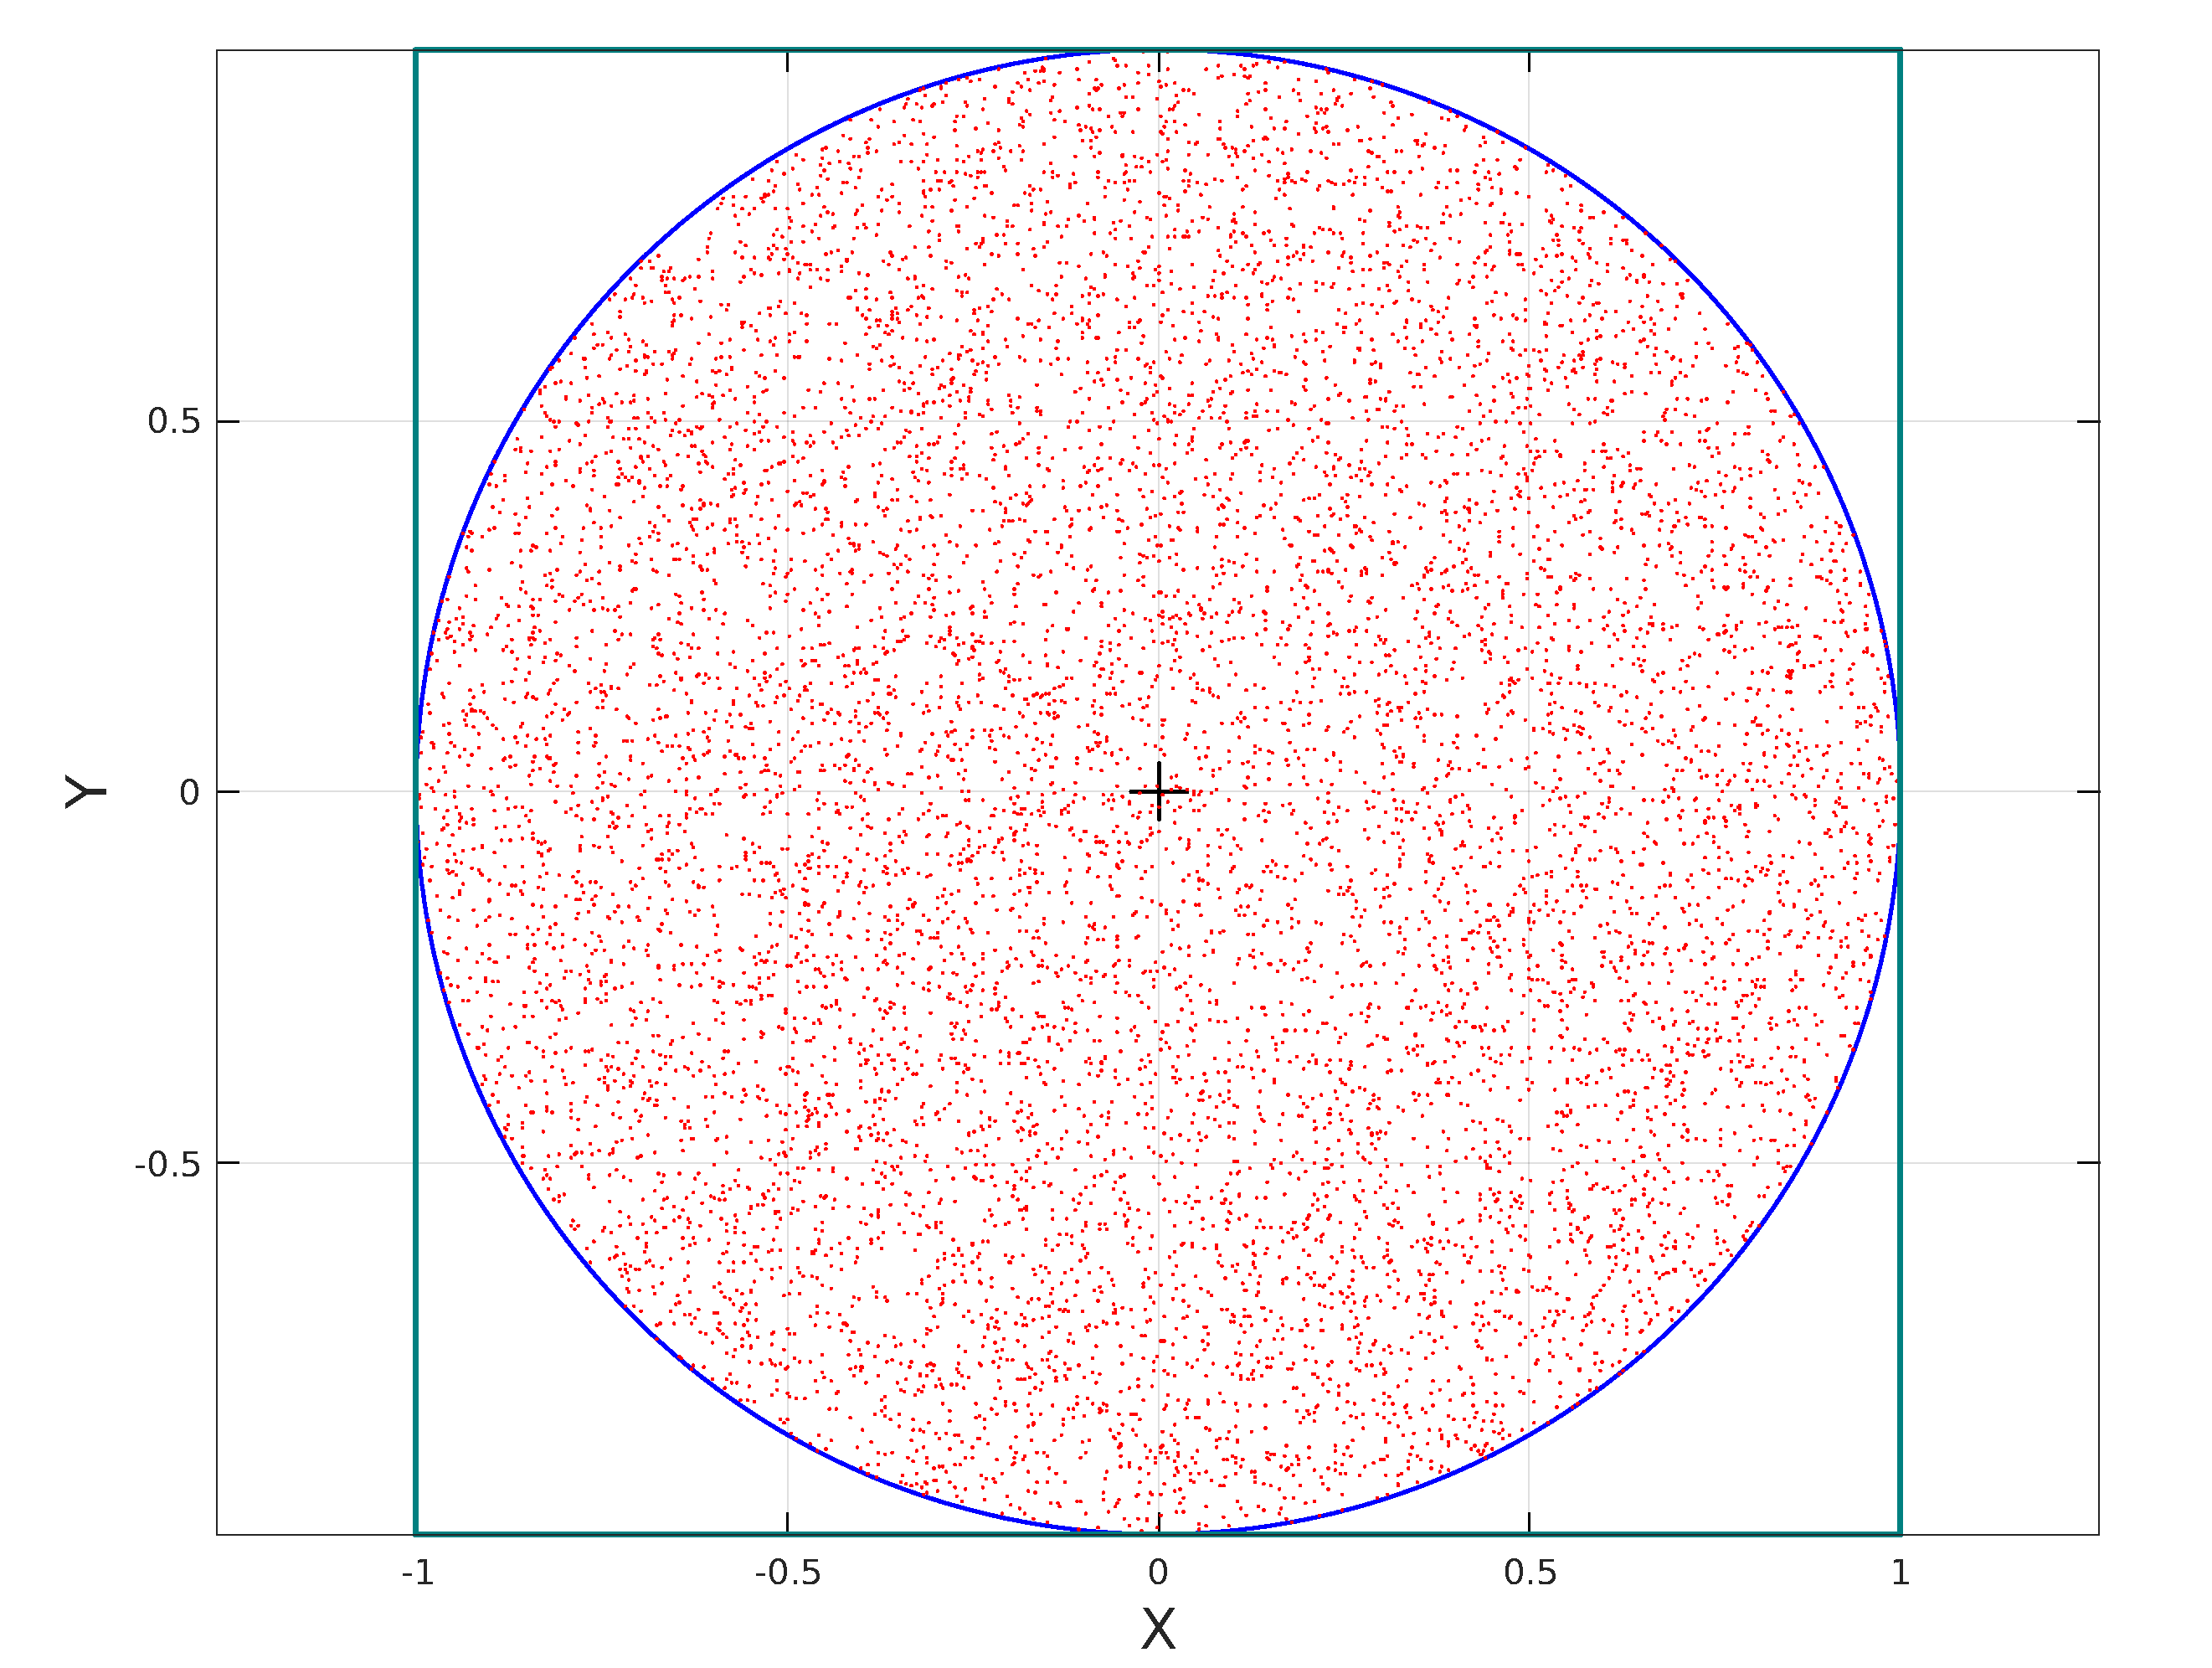
\includegraphics[scale=0.3]{sources/random_points_in_circle/images/loop_points}
	\caption{Large number of points generated using the approach described in Section \ref{random_points_in_circle:sec:loop}.}
\end{figure}

\subsection{Brute-force}
\label{random_points_in_circle:sec:bruteforce}

\lstinputlisting[language=c++, caption=Sample Caption,label=list:random_points_in_circle]{sources/random_points_in_circle/random_points_in_circle_solution1.cpp}


%!TEX root = ../main.tex
%%%%%%%%%%%%%%%%%%%%%%%%%%%%%%%%%%
% Links:
%
% Difficulty:
% Companies: 
%%%%%%%%%%%%%%%%%%%%%%%%%%%%%%%%%%

\chapter{Best time to buy and sell stock}
\label{ch:buy_sell_stocks}
\section*{Introduction}
The problem discussed in this chapter is not particularly difficult as it is easily solvable in quadratic time using a brute-force algorithm. 
However, a more efficient solution is possible and, given that this is exactly the type of question for which interviewers expect fast and elegant solutions, it's worth taking the time to become familiar with the problem structure and the best approaches to solving it.  

\section{Problem statement}
\label{sec:buy_sell_stocks:statement1}
\begin{exercise}
You are given prices for a stock for a number $n$ of days. The prices are stored in an array $P$ of length $n$ where each cell $i$ of the array contains the price for the stock on the $i^{th}$ day. You are only permitted to perform \textbf{one} buy and \textbf{one} sell operations. What is the maximum profit you can achieve given the prices for the stock in $P$?

You have to perform the buy operation \textbf{before} the sell operation. You cannot buy the stock on the \nth{10} day and sell on the \nth{9}.

\begin{example}
	\hfill \\
	Given the array of prices for the stock is: $[7,1,5,3,6,4]$, the answer is $5$. You can buy on the \nth{2} day and sell on the \nth{5}.
\end{example}

\begin{example}
	\hfill \\
	Given the array of prices for the stock is: $[6,5,4,3,2,1]$, the answer is $0$. There is no way you can make a profit higher than $0$ i.e. not buying and not selling. 
\end{example}

\end{exercise}

\section{Clarification Questions}

\begin{QandA}
	\item \begin{questionitem} \begin{question} Can you perform the buy and sell operation on the same day?  \end{question}      
    \begin{answered}
		\textit{Yes, that is possible.}
	\end{answered} \end{questionitem}
\end{QandA}

\section{Discussion}
\label{buy_sell_stocks:sec:discussion}
A profit is achieved when a buy and sell transaction are performed with prices $p_b$ and $p_s$ respectively and $p_b \leq p_s$. In other words, our goal is to buy at a lower price than we sell. The maximum profit is obtained whenever the spread between those two prices is maximum i.e. $\max_{}{(p_s - p_b)}$

\subsection{Brute-force}
\label{buy_sell_stocks:sec:bruteforce}
The brute force approach is very straightforward as the only thing we need to do is apply the definition of maximum profit we discussed earlier. For all pairs of ordered index $i \leq j$ we can calculate $P_i - P_j$ and return the maximum among all those profit values. Listing \ref{list:buy_sell_stocks:bruteforce} shows an implementation of this approach. Note that a profit of $0$ is always possible by either not performing any transaction or simply performing the buy and sell on the same day. Thus $j = i+1$, because it is pointless to calculate the profit for the same day as we know already it will always be $0$. For this reason we also limit the buy operation to the day before ($i< n-1$) the last, because if we want to have any chance of making a profit we need to at least have one day left after the buy to perform the sell operation. 

\lstinputlisting[language=c++, caption={Brute force $O(n^2)$ solution to the problem of buying and selling stock.},label=list:buy_sell_stocks:bruteforce]{sources/buy_sell_stocks/buy_sell_stocks_solution1.cpp}

\subsection{Linear time solution}
\label{buy_sell_stocks:sec:linear}
The solution above can be improved if we look at the problem from slightly different angle. The idea is that we can process the array from the last day to the first and, for each of the days, calculate the \textbf{best} profit to be made by selling on any of the days already processed (which occurs later in time).

We keep a variable $b$ with the maximum price seen so far which is initially $-\infty$. The algorithm starts from day $n$ and for each day checks whether buying that day and selling at the price $b$ (the highest price seen so far) would improve the profit found thus far. This approach is correct because the maximum profit happens when the spread between sell and buy price is maximum.
The implementation of the idea above is shown in Listing \ref{list:buy_sell_stocks:linear}.

\lstinputlisting[language=c++, caption={Dynamic programming linear time, constant space solution to the problem of buying and selling stock.},label=list:buy_sell_stocks:linear]{sources/buy_sell_stocks/buy_sell_stocks_solution2.cpp}


%Multiple transaction variation
\section{Common Variations - Multiple Transactions}
\label{sec:buy_sell_stocks:multiple_transaction}

\subsection{Problem statement}
\begin{exercise}
	You are given an integer array $P$ where $P[i]$ contains the price of a given stock on the $i^{th}$ day.

	On each day, you may decide to buy and/or sell the stock. 
	You can only hold at most one share of the stock at any given time.
	However, you might engage in multiple transaction over the course of time i.e. you repeat the process of buying a share then sell it after a while (also the next day) multiple times.
	
	Write a function that given $P$ returns the maximum profit achievable.

	Notice that you may not engage in multiple transactions at the same time i.e., you must sell the stock before you buy it again.
	\begin{example}
	\label{ex:buy_sell_stocks_2:exmaple1}
		\hfill \\
		Given the array of prices for the stock is: $[7,1,5,3,6,4]$, the answer is $7$. 
		You can buy on the \nth{2} day and sell on the \nth{3} and then engage on a second transaction where you buy on the \nth{4} day and sell on the \nth{5}.
	\end{example}

\end{exercise}


\section{Discussion}
\label{buy_sell_stocks_2:sec:discussion}
This might seems like an harder problem at first than the version presented in Section \ref{sec:buy_sell_stocks:statement1} but in reality as we will see in Section \ref{buy_sell_stocks_2:sec:linear} its solution is actually easier.

\section{Brute force solution}
\label{buy_sell_stocks_2:sec:bruteforce}
As usual we start our discussion by quickly presenting the brute force solution. In this case this means trying all possible sets of transactions (a valid pair of buy and sell operation not overlapping with any other transaction). We can try all possible sets by using recursion cleverly. However this approach will not take us far because the number of possible sets of transaction grows exponentially.
We are showing this approach in Listing \ref{list:buy_sell_stocks_2:bruteforce}  only because we think its implementation can be somehow instructive.

\lstinputlisting[language=c++, caption={Bruteforce exponential solution to the problem of buying and selling stock with no limits on the number of transactions.},label=list:buy_sell_stocks_2:bruteforce]{sources/buy_sell_stocks/buy_sell_stocks_2/buy_sell_stocks_2_solution1.cpp}

\section{Linear time solution}
\label{buy_sell_stocks_2:sec:linear}


The idea is simple and it is clearer once we look at prices plotted on a graph. As you can see in Figure \ref{}, the data is made of peaks and valleys (unless the data is fully increasing or decreasing). Those are the point of interests because if we buy at valleys and sell at peaks we are able to obtains the maximum profit. 
One can simply loop thought the array and identify those peaks and valleys and calculate the total profit as the sum of the profits along those point of interests. 
For instance w.r.t. the example \ref{ex:buy_sell_stocks_2:exmaple1} there are two pairs  valley-peak happening at days $2$ and $3$ and days $4$ and $5$, respectively. 
But, what is a valley and/or a peak exactly?
A day $i$ is a valley if $P_i < P_{i-1}$ and $P_i > P_{i+1}$
while is a peak if $P_i > P_{i-1}$ and $P_i < P_{i+1}$.
So all it is needed is to identify those pairs of valleys and peaks and we are done. 

But do we really need to find peaks and valleys? The answer is not as all it is necessary is to make sure we cash at \textbf{all} opportunities we have i.e. in all those cases where we can buy at a lower price we sell. Thus we can process days two at the time and, since there is no limit on the number of transactions, simply buy and sell whenever the spread between buy and sell price is convenient. 

The idea above can be implemented as shown in Listing \ref{list:buy_sell_stocks_2:linear}. 


\lstinputlisting[language=c++, caption={$O(n)$ time and $O(1)$ space solution to the problem of buying and selling stock with no limits on the number of transactions.},label=list:buy_sell_stocks_2:linear]{sources/buy_sell_stocks/buy_sell_stocks_2/buy_sell_stocks_2_solution2.cpp}

%!TEX root = ../main.tex
%%%%%%%%%%%%%%%%%%%%%%%%%%%%%%%%%%
% Links:
%
% Difficulty: Companies: 
%%%%%%%%%%%%%%%%%%%%%%%%%%%%%%%%%%

\chapter{Find the cycle in a Linked list}
\label{ch:cycle_in_list}
\section*{Introduction}
The problem described in this chapter is a classical one that has been reported to be asked in 
in countless coding interviews. The topic of this chapter is linked-lists: linear collections of elements whose order, unlike an array,
is not dictated by their ordering in memory. 
By being one of the most simple and common data structures you can expect them to be as important for your interview preparation.

The major difference that lists offer over conventional arrays is that elements in the list can be efficiently  (in constant time) 
removed and inserted without the need to reorganize and perform a complete restructuring of the whole data \footnote{For arrays, the cost of inserting or deleting an element is linear as you need to:
\begin{enumerate*}
	\item possibly enlarge the allocated space for the array
	\item copy all the elements (minus or plus the element you want to remove or insert) in the new memory space
\end{enumerate*}.
}. Because of this property linked lists are often used to implement more complex data structures 
where this insertion and deletion cost is crucial, for example associative arrays.
There are however quite a few drawbacks associated with them, for instance:
\begin{enumerate*}
	\item memory consumption (as for each node of the list you also pay a price as has to remember the next and/or previous nodes).
	\item they offer sequential access. Accessing a node costs linear time.
	\item cache unfriendly
\end{enumerate*}. This is the reason why  

A linked list is, at a high level of abstraction, a collection of so-called nodes or elements  each of them (except the last) containing
a pointer to the next one. 
Each node also carries payload data, which is the information you want ultimately to be stored.
The standard linked lists has two special nodes:
\begin{itemize}
	\item the head that is not pointed by other elements and is the first of the collection. 
	\item the tail, which is a node that has no next element, and is, not surprisingly, the last of the elements.
\end{itemize}

In some particular cases during the manipulation of the list you might end up with a broken or corrupted one  where the tail node does not exists anymore, meaning that
each of the elements in the list is pointing to some other nodes.
In this situation a loop forms and the list becomes what it known as a \textit{circular} list.
In this chapter we will investigate how we can find out whether:
\begin{enumerate*}
	\item a list is circular, and when it is,
	\item how to identify the first element of the loop.
\end{enumerate*}.

\section{Problem statement}
\begin{exercise}
Given a singly linked list (definition in Listing \ref{list:delete_duplicates_list:linked_list} at
page \pageref{list:delete_duplicates_list:linked_list}) determine whether the list contains a loop.
\begin{itemize}
		\item If it does, return the the node where the loop starts
		\item otherwise, return \lstinline[columns=fixed]{nullptr}
\end{itemize}

For the rest of the chapter we will use an array of integers to represents the nodes of the list and
a single integer to represent the node the last element of the list connects to, in order to create
a cycle or $-1$ if there is no cycle. For instance  the array $L=[1,2,3,4]$ and the integer $2$
represent the list shown in Figure \ref{fig:cycle_in_list:example1}.

\begin{example}
	\hfill \\
	Given the List $\{[1,2,3,4,5],2\}$, the function returns the address of the node $2$. See Figure
	\ref{fig:cycle_in_list:example1}.
\end{example}

\begin{example}
	\hfill \\
	Given the List $\{[1,2,3,4,5],-1\}$, the function returns \inline{nullptr}. See Figure
	\ref{fig:cycle_in_list:example2}.
\end{example}
\end{exercise}

\begin{figure}
	\centering
	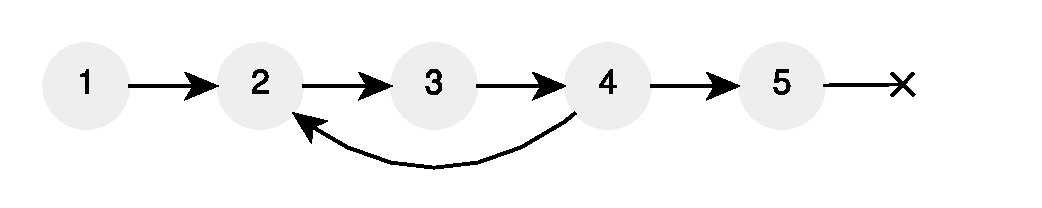
\includegraphics[scale=1.0]{sources/cycle_in_list/images/list_cycle}
	\caption{Example of linked list with a cycle.}
	\label{fig:cycle_in_list:example1}
\end{figure}
\begin{figure}
	\label{fig:cycle_in_list:example2}
	\centering
	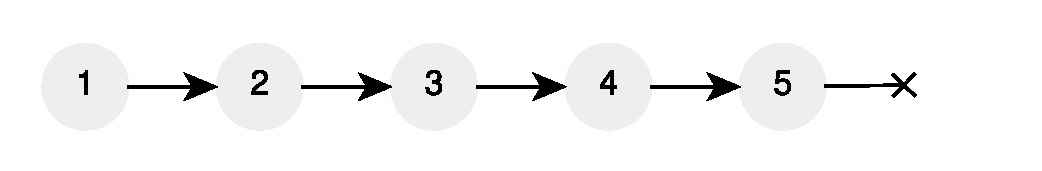
\includegraphics[scale=1.0]{sources/cycle_in_list/images/list_no_cycle}
	\caption{Example of linked list with no cycle.}
\end{figure}

%\section{Clarification Questions}
%
%\begin{QandA} \item \begin{answered} \textit{} \end{answered}
%
%\end{QandA}

\section{Discussion}
\label{cycle_in_list:sec:discussion}
Considering this is a very well-known problem we will not spent time on dwelling on naive
brute-force solution, and instead will only concentrate first on an optimal in time solution with
linear space, and then we will concentrate on improving it by lowering the space complexity to
constant. 

All solution implementation in this chapter uses the  Linked list definition shown in Listing \ref{list:cycle_in_list:node_definition};

\begin{minipage}{\linewidth}
	\lstinputlisting[language=c++, caption={Singly linked-list node definition.},label=list:cycle_in_list:node_definition]{sources/cycle_in_list/linked_list.h}
\end{minipage}

\subsection{Linear time and space solution}
\label{cycle_in_list:sec:bruteforce}
This problem has many similarities with the problem of finding a duplicate in a collection and can
therefore be solved using a similar approach. The idea is to visit the list and store in a hash-set
the  address of the node \textbf{already} visited. While visiting a new node, we first check if that
node was already visited, and if yes, it means that we can stop because we found the starting point
of a loop. If we reach the end of the list and we were not be able to find a duplicate, then it
means there is no loop and we can return \lstinline[columns=fixed]{nullptr}. A possible
implementation of this idea is shown in Listing \ref{list:cycle_in_list:linearspace}.

\lstinputlisting[language=c++, caption={Linear time and space solution to the problem of detecting a cycle in a linked list where an hashset is used to remember already visited nodes.},label=list:cycle_in_list:linearspace]{sources/cycle_in_list/cycle_in_list_solution1.cpp}



\subsection{Slow and fast pointer solution - Floyd’s algorithm }
\label{cycle_in_list:sec:slowfast}
This algorithm\cite{cit::wiki::floyd} uses the fact that, like clock's hands, things iterating on a
cycle at different speeds will eventually meet at some point in the future. Consider two runner $R_1$
and $R_2$ with velocities $V_1$ and $V_2=2V_1$ respectively ($R_2$ goes twice as fast then $R_1$),
starting their run from the same point in a circular stadium. They will meet again when the slower
runner reach the starting point for the second time. Why? By the time the slower one has completed
half circle the faster has completed a complete cycle and by the time the slower finishes his run,
arriving at the starting point again, the faster has completed a second entire cycle. We can use
this fact to detect a cycle in a linked list even if for the cycle detection problem things might be
a bit more complicated because the two runners might now start going in loop at the same time (the
list potentially has a first part the is not part of the loop as can be seen in Figure
\ref{fig:cycle_in_list:example1}). 


The rest of the section is a bit technical and you can skip to
the implementation shown in Listing \ref{list:cycle_in_list:constantspace} which can be self-explanatory considering that in the end the intuition behind the algorithm is quite easy. If you
are interested in the details of why it works, read along. 


Consider two iterators p,q with velocities $v_p=1$,$v_q=2$  respectively. Suppose the
\textbf{cycle}(not the entire list) has length $n$. We can have two scenarios depending on the index
$A$ of the starting node of the cycle:

\begin{enumerate}
\item the cycle starts at $A < n$.
\item or  starts at \(A \geq n\).
\end{enumerate}
For the case $(1)$ when the slower iterator reaches $A$ the faster is at location $2A$ (which might
mean that the faster iterator looped around the cycle already). How many iterations $k$ it will take
before they meet? And at which node?
The situation is described by the following congruences:
\begin{align}
  A + kv_p &\equiv 2A + k2v_p \Mod{n} \\
  2A + k2v_p &\equiv A + kv_p \;  \Mod{n} \\
  A + k2v_p &\equiv kv_p   \Mod{n} \\
  A +kv_p &\equiv 0   \Mod{n} \\
  A +k &\equiv 0  \Mod{n}
\end{align}
which has solution \(k = n-A\). This means that they will meet after \(k=n-A\) iterations of the
slower iterator, i.e. at \(A\) nodes before the beginning of the cycle and we can use this fact to
count \(A\) nodes from the beginning of the list so to find the starting point of the cycle. 

So, once the iterators meet \textbf{in the cycle}, we can move the fast iterator back to the
beginning of the list and iterate forward one node per step with both iterators until they match
again. When we move the fast iterator back at the head of the list, \textbf{both iterators are \(A\)
nodes away from the beginning of the cycle}. Because of this, when we move both of them by one, they
will eventually meet exactly at that node \(A\) i.e. the beginning of the cycle.

%%%------------

Let's consider now the case ($2$) i.e.  when \(A \geq n\). This means that by the time the slower
iterator reaches the beginning of the cycle the faster one has completed more that a cycle. What
will be the starting point for the faster one? We argue that once \(p\) reaches \(A\), \(q\) is at
node \(2A\) but since \(A > n\), this means that it will be at position \(A + (A \Mod{n})\). We can
now use similar argument to the previous case and write:

\begin{align}
  A + kv_p &\equiv A + (A \Mod{n}) + (k2v_p \Mod{n}) \\
  A + (A \Mod{n}) + k2v_p &\equiv A + kv_p\;\Mod{n} \\
  (A \Mod{n}) + kv_p \Mod{n} & \equiv 0\Mod{n} \\
  (A \Mod{n}) + k \Mod{n} &\equiv 0 \Mod{n} \: \: \text{  : because  } v_p=1 \\
\end{align}
which has solution \(k = n-(A \Mod{n})\). This means that the meeting point is \(A \Mod{n}\) nodes
before the beginning of the cycle. If we do the same operations as the previous case,(when \(A <
n\)), we obtain again, the same result. Iterators will meet at the beginning of the cycle. Why? Well
advancing \(q\) makes \(p\) cycle possibly several times ( remember that \(A \geq n\)  ) and it will
clearly stops at \( A+(n-A \Mod{n}) + A \Mod{n} = A +n \;(mod (n))= A\).
In other words the slower pointer is at first  at node number \(A+(n-A \Mod{n})\). We can write \( A
= bn + r\) where \(r = A \;\Mod{n}\). After \(A\) advancing steps it will be at location  \( A+(n-A
\;\Mod{n}) +bn +r (\Mod{n})\). Since \(bn \; \Mod{n}=0\) the result follows.

As an example consider a list with a cycle of length \(n=4\) starting at node number \(10\). The
first part of the algorithm tells us that the nodes will meet at node \(10 + 4 - 10 \: mod(4) =
12\). Moving the fast pointer back to the head of the list and iterating one node per time both
iterators will lead the slower point to node:


Figure \ref{fig:cycle_in_list:floyd} depicts how the algorithm
works on a list of $8$ nodes with a cycle of length $4$ starting at node number $4$. 
After $5$ steps the slow ($p$) and fast ($q$) iterators point to the same node i.e. node number $6$. 
After a new phase starts, with the slow pointer being moved to the head of the list and continues with both iterators moving forward by $1$
until they meet again. 
They will meet again at the beginning of the cycle. 

An implementation of the Floyd's algorithm is shown in Listing \ref{list:cycle_in_list:constantspace}.
\lstinputlisting[language=c++, caption={Floyd's algorithm, linear time, constant space solution to the problem of detecting a cycle in a linked list.},label=list:cycle_in_list:constantspace]{sources/cycle_in_list/cycle_in_list_solution2.cpp}


%\begin{figure}[htbp]
	%\label{fig:cycle_in_list:flow1} \centering
	%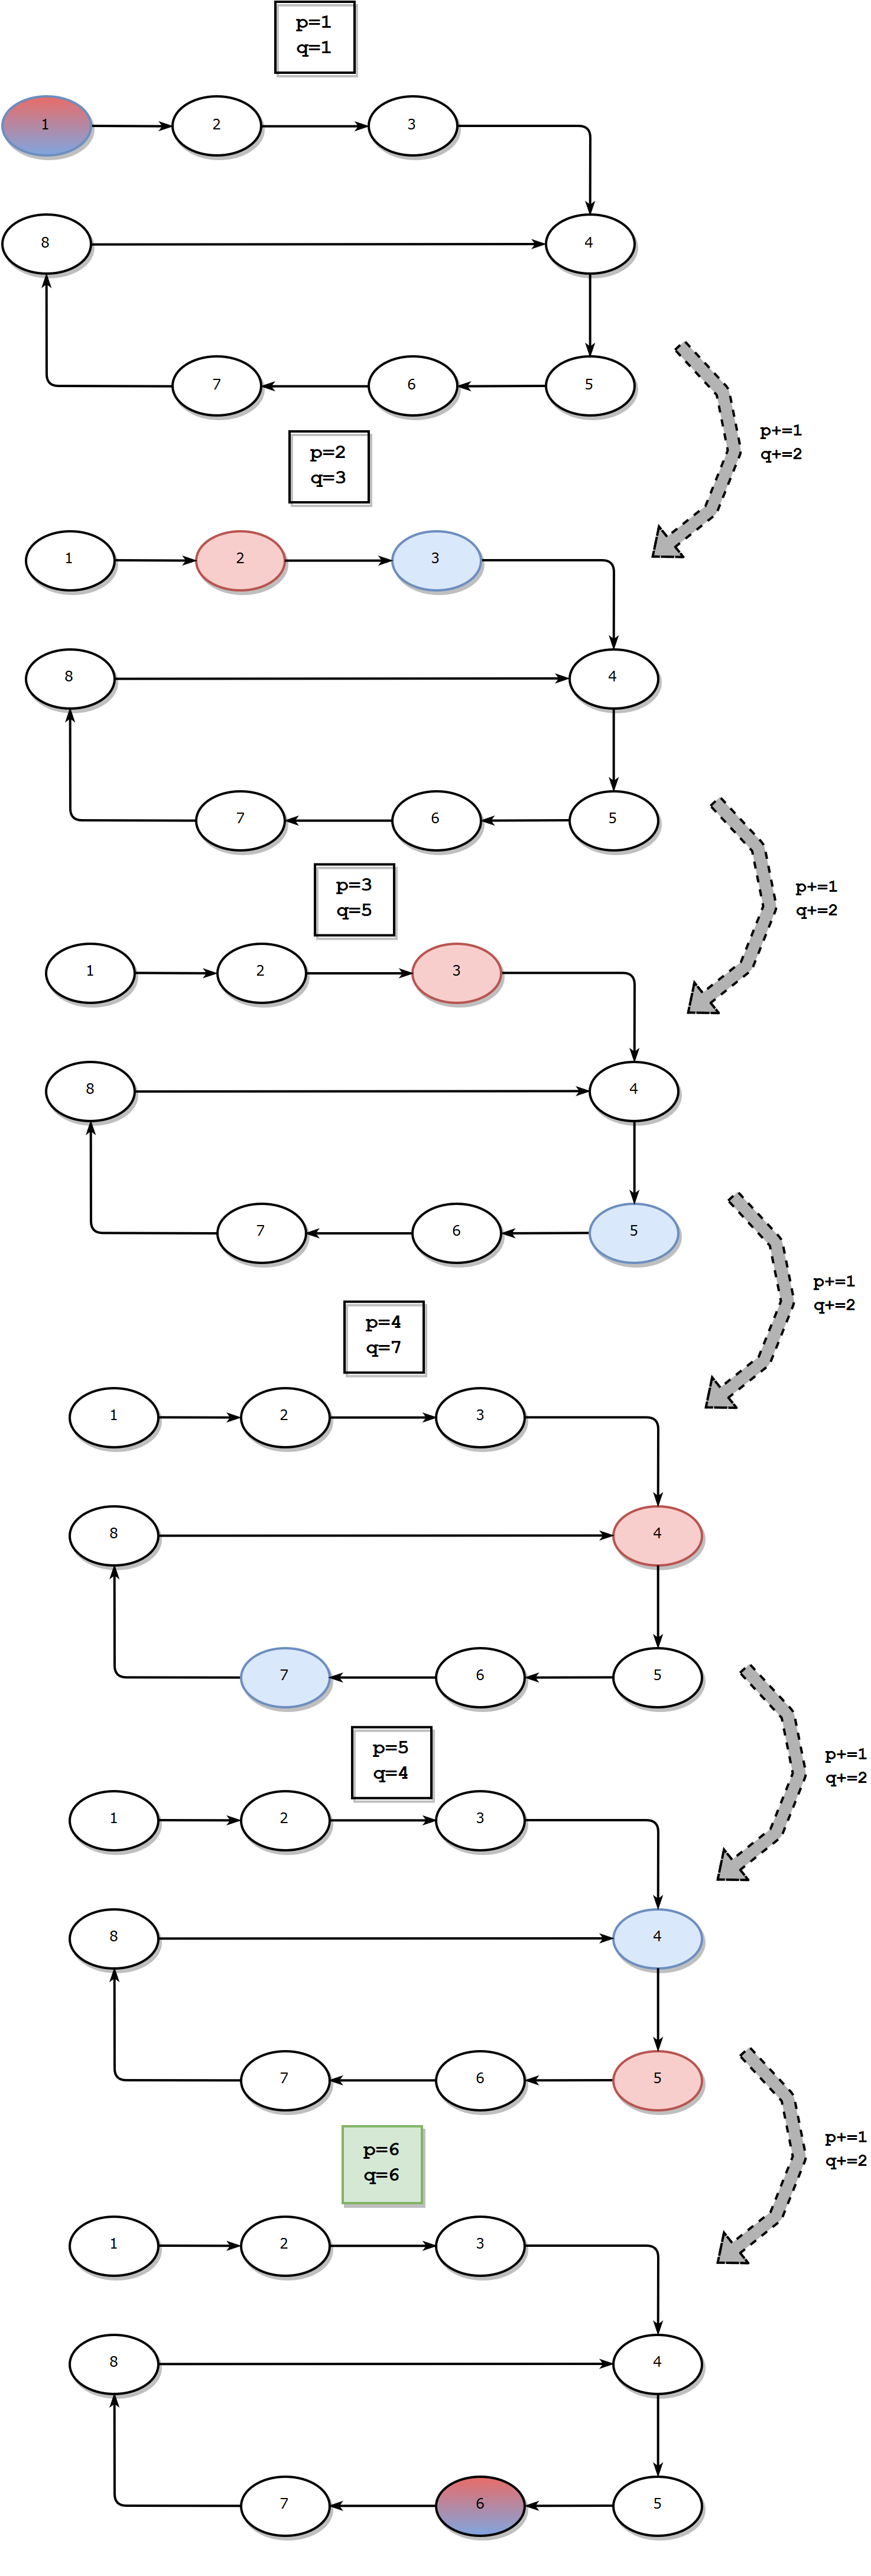
\includegraphics[scale=0.15]{sources/cycle_in_list/images/flow1} \caption{Execution of the
	%first phase of the Floyd's algorithm on a list of $8$ nodes with a cycle of length $4$ starting
	%at node $4$.}
%\end{figure}

%\begin{figure}[htbp]
	%\label{fig:cycle_in_list:flow2} \centering
	%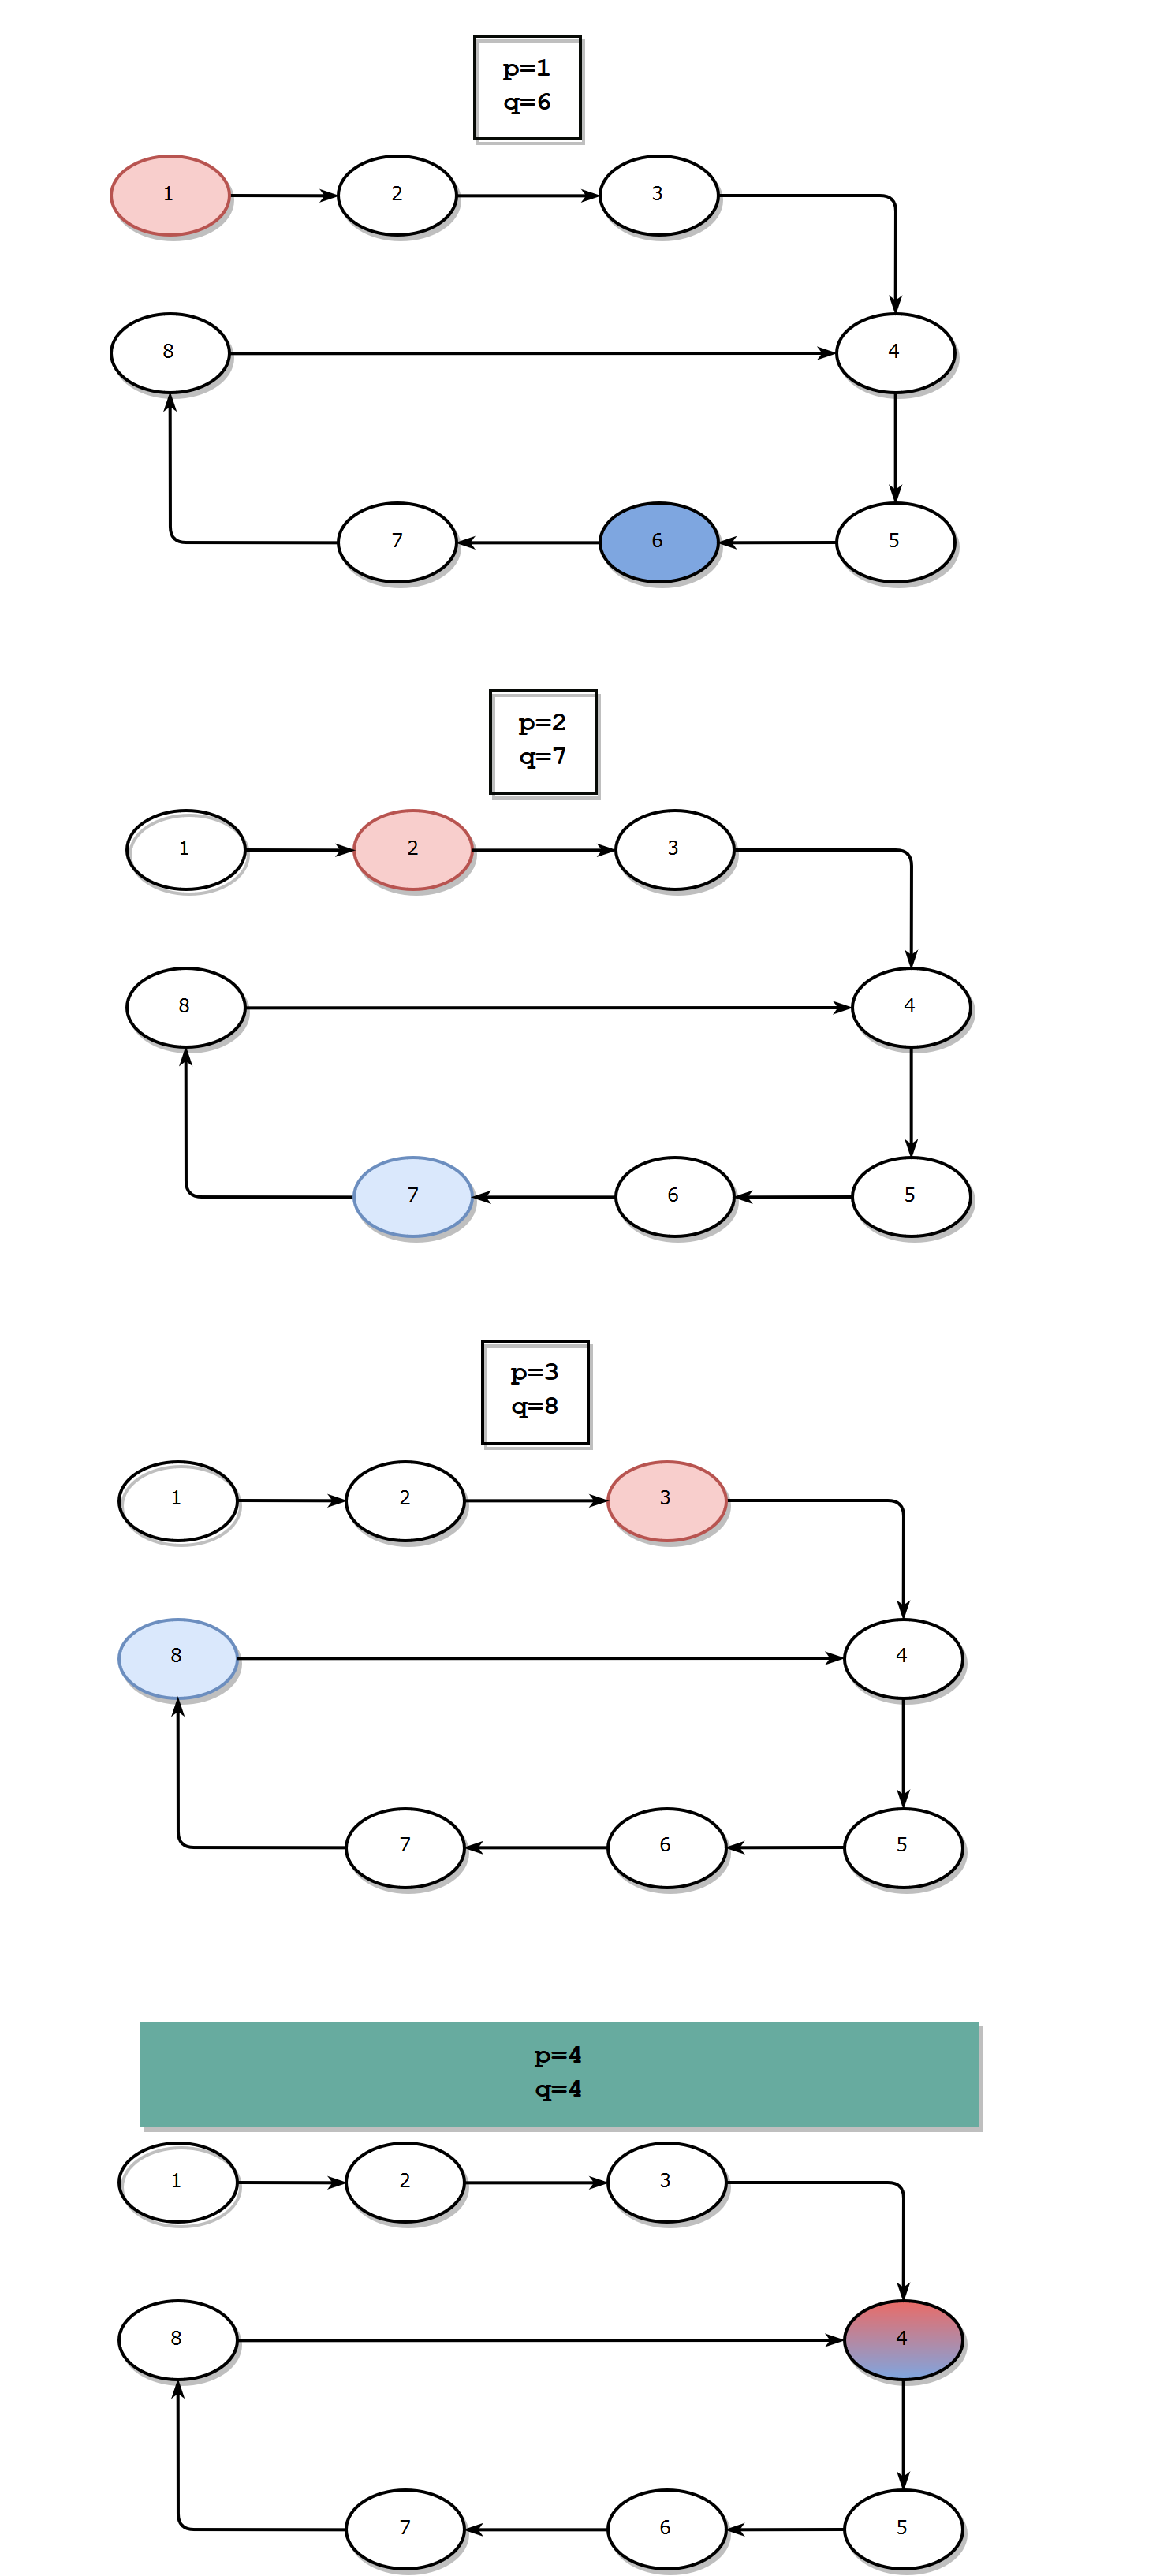
\includegraphics[scale=0.15]{sources/cycle_in_list/images/flow2} \caption{Execution of the
	%second phase of the Floyd's algorithm on a list of $8$ nodes with a cycle of length $4$
	%starting at node $4$.}
%\end{figure}




\begin{figure}
	\vspace*{-0.5in}
	\centering
	\begin{subfigure}[t]{0.36\textwidth}
		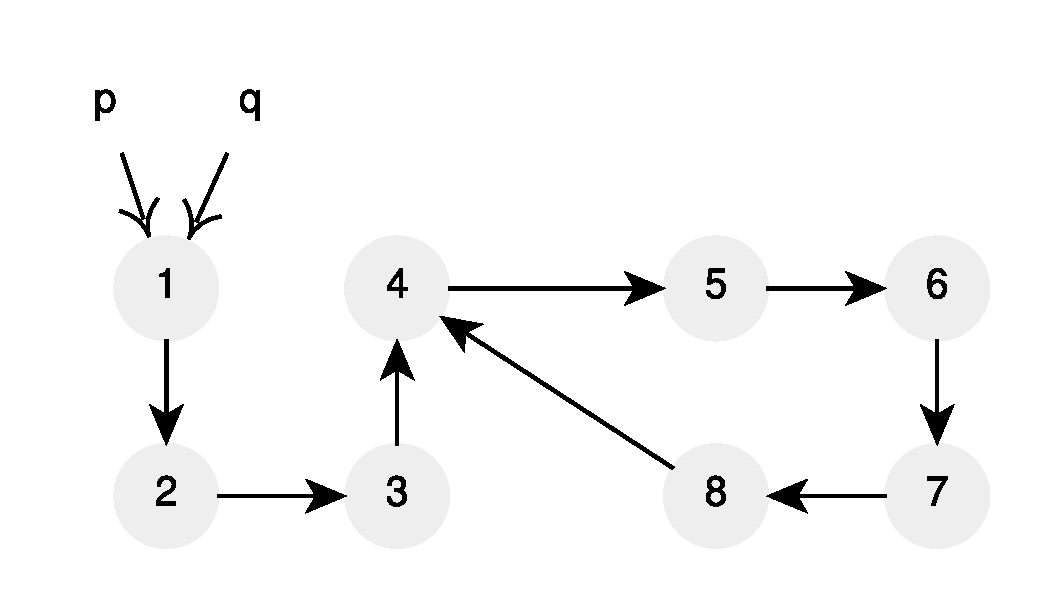
\includegraphics[width=1\linewidth]{sources/cycle_in_list/images/floyd1}
		\caption{At the beginning $p=q=1$. The slow and fast forward: $p=p+1$, $q=q+2$.}
		\label{fig:cycle_in_list:floyd1}
	 \end{subfigure}
	\hfill
	\begin{subfigure}[t]{0.36\textwidth}
		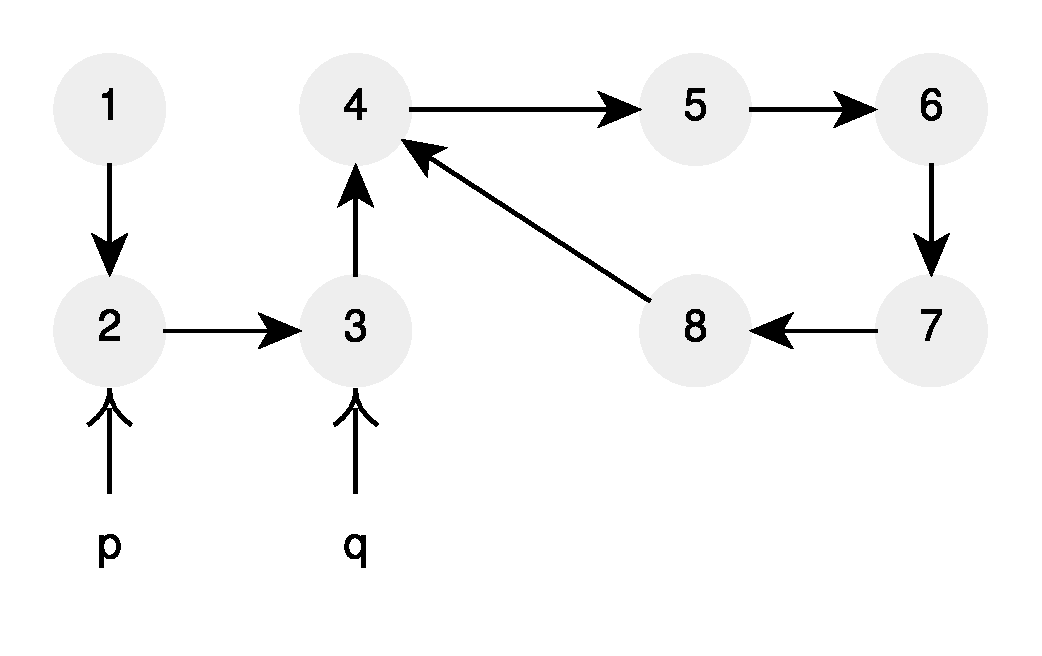
\includegraphics[width=1\linewidth]{sources/cycle_in_list/images/floyd2}
		\caption{$p \neq q$,  thus: $p=p+1$, $q=q+2$}
		\label{fig:cycle_in_list:floyd2}
	 \end{subfigure}
	 \hfill
	 \begin{subfigure}[l]{0.36\textwidth}
		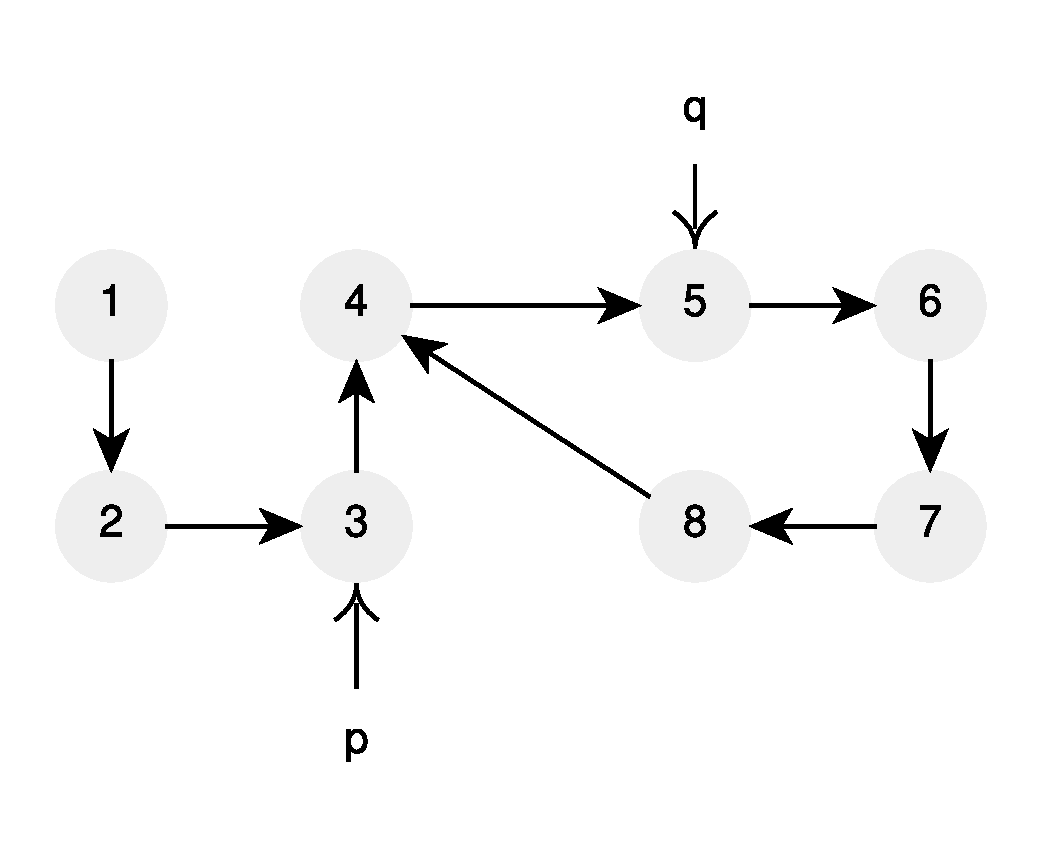
\includegraphics[width=1\linewidth]{sources/cycle_in_list/images/floyd3}
		\caption{$p \neq q$,  thus: $p=p+1$, $q=q+2$}
		\label{fig:cycle_in_list:floyd3}
	 \end{subfigure}
	 \hfill
	 \begin{subfigure}[l]{0.36\textwidth}
		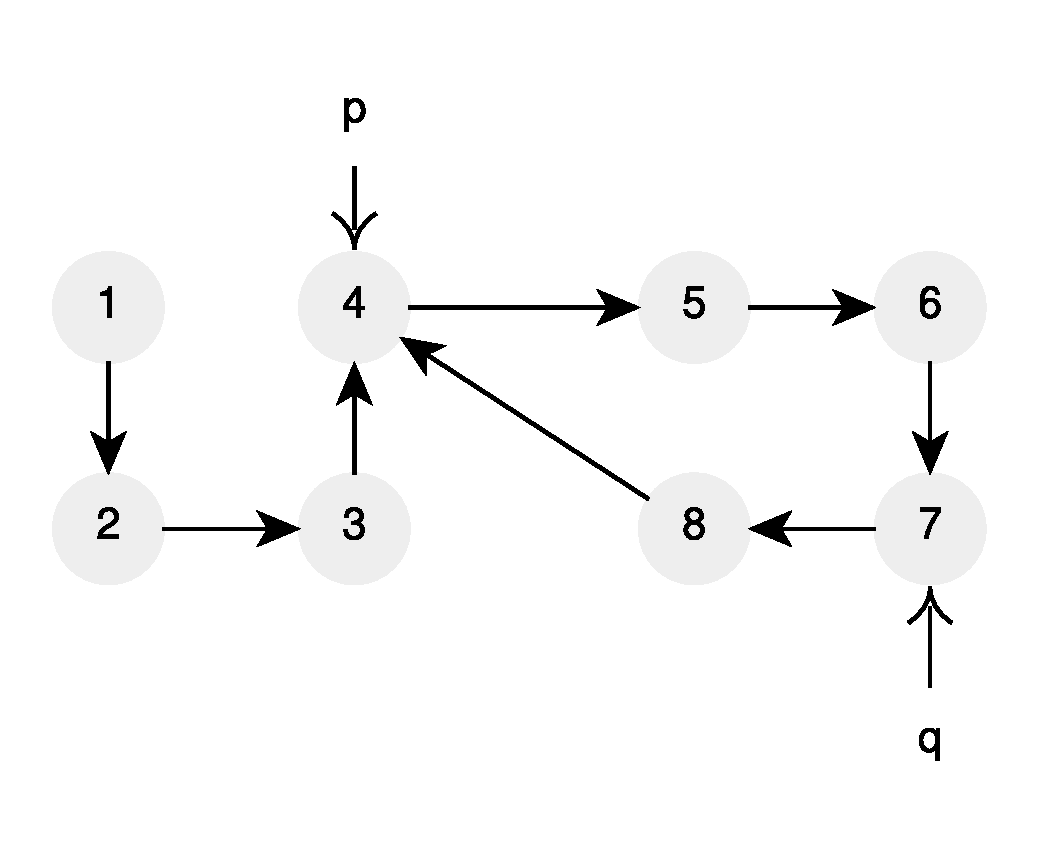
\includegraphics[width=1\linewidth]{sources/cycle_in_list/images/floyd4}
		\caption{$p \neq q$,  thus: $p=p+1$, $q=q+2$}
		\label{fig:cycle_in_list:floyd4}
	 \end{subfigure}
	 \hfill
	 \begin{subfigure}[l]{0.36\textwidth}
		\includegraphics[width=1\linewidth]{sources/cycle_in_list/images/floyd5}
		\caption{$p \neq q$,  thus: $p=p+1$, $q=q+2$}
		\label{fig:cycle_in_list:floyd5}
	 \end{subfigure}
	 \hfill
	 \begin{subfigure}[l]{0.36\textwidth}
		\includegraphics[width=1\linewidth]{sources/cycle_in_list/images/floyd6}
		\caption{$p = q$. The fast and slow movements stop.}
		\label{fig:cycle_in_list:floyd6}
	 \end{subfigure}
	 \hfill
	 \begin{subfigure}[l]{0.36\textwidth}
		\includegraphics[width=1\linewidth]{sources/cycle_in_list/images/floyd7}
		\caption{$p$ is reset to the beginning of the list. $q$ is not moved.  
		From now on $p$ and $q$ are moved one step at the time.}
		\label{fig:cycle_in_list:floyd7}
	 \end{subfigure}
	 \hfill
	 \begin{subfigure}[l]{0.36\textwidth}
		\includegraphics[width=1\linewidth]{sources/cycle_in_list/images/floyd8}
		\caption{$p \neq q$,  thus: $p=p+1$, $q=q+1$}
		\label{fig:cycle_in_list:floyd8}
	 \end{subfigure}
	 \hfill
	 \begin{subfigure}[l]{0.36\textwidth}
		\includegraphics[width=1\linewidth]{sources/cycle_in_list/images/floyd9}
		\caption{$p \neq q$,  thus: $p=p+1$, $q=q+1$}
		\label{fig:cycle_in_list:floyd9}
	 \end{subfigure}
	 \hfill
	 \begin{subfigure}[l]{0.36\textwidth}
		\includegraphics[width=1\linewidth]{sources/cycle_in_list/images/floyd10}
		\caption{$p = q$. The algorithm stops, and both $p$ and $q$ point to the beginning of the cycle.}
		\label{fig:cycle_in_list:floyd10}
	 \end{subfigure}
	 \caption[Execution of the Floyd’s algorithm]{Execution of the Floyd’s algorithm. The slow and
	  fast pointers are initialized to the head of the list (see Figure
	  \ref{fig:cycle_in_list:floyd1}) and immeditely moved forward at different speeds (Figure
	  \ref{fig:cycle_in_list:floyd2}). They continue to move forward at different speed until their
	  values mismatch (from Figure \ref{fig:cycle_in_list:floyd2} to
	  \ref{fig:cycle_in_list:floyd6}). At this point $p$ is moved back to the head of the list
	  (Figure \ref{fig:cycle_in_list:floyd7}). From now on the pointers are moved at the same speed
	  of $1$ and they continue to move forward until they match again (from Figure
	  \ref{fig:cycle_in_list:floyd8} to \ref{fig:cycle_in_list:floyd10}.). $p$ and $q$ now point to
	  the beginning of the cycle in the list.}
	  \label{fig:cycle_in_list:floyd}
\end{figure}

%!TEX root = ../main.tex
%%%%%%%%%%%%%%%%%%%%%%%%%%%%%%%%%%
% Links:
%
% Difficulty: Companies: 
%%%%%%%%%%%%%%%%%%%%%%%%%%%%%%%%%%

\chapter{Reverse a singly linked list}
\label{ch:list_reverse}

\section*{Introduction}
In this chapter we are going to have a look at a problem based on reversing a singly linked list. Despite the fact that this is one of the fundamental structures in computer science and is also an extremely popular interview question, it often trips up prospective candidates and is usually a cause for immediate rejection. As such, it is worth spending a bit of time on it to ensure a solid grasp of the optimal solutions. 

The problem has  a simple definition as all it asks us to do is reverse a given list.
We will discuss how we can approach this problem both a recursive and an iterative
manner. We will also examine a slightly harder variation that is
often asked as a follow-up although we leave the solution to that one for the reader. 


\section{Problem statement}
\begin{exercise}
Create a function that,  given a singly linked list $L$, reverses it and return the pointer to the new
head of $L$. $L$ is given as a pointer to the first node of the list. The definition of the node is
given in Listing \ref{list:list_reverse:node_definition}.



\begin{example}
	\hfill \\
	Given the $L = 1 \rightarrow 2 \rightarrow 3 \rightarrow 4 \rightarrow 5$, the function modifies
	it into $L = 5 \rightarrow 4 \rightarrow 3 \rightarrow 2 \rightarrow 1$ and returns a pointer to
	the node $5$, the new head of the list.
\end{example}

\end{exercise}

\lstinputlisting[language=c++, caption={Singly linked-list node definition.},label=list:list_reverse:node_definition]{sources/cycle_in_list/linked_list.h}

\section{Clarification Questions}

\begin{QandA}
	\begin{questionitem} \begin{question} Can the input list be empty?   \end{question} 	 
    \begin{answered}
		\textit{Yes.}
	\end{answered} \end{questionitem}

	\begin{questionitem} \begin{question} Can I assume $L$ is not corrupted by e.g. containing cycles?   \end{question} 	 
    \begin{answered}
		\textit{Yes, the input list is a singly linked list with no cycles.}
	\end{answered} \end{questionitem}
	
\end{QandA}

\section{Discussion}
\label{list_reverse:sec:discussion}
Solving this problem using linear additional space is trivial as we can iterate over the list
and for each push the address of each of its nodes in a stack. We can then pop them one at a time
while making sure they are connected in the same order they are popped out. Listing
\ref{list:list_reverse:stack} shows a possible implementation of this idea. The time and space
complexity of this approach is $O(n)$.

\lstinputlisting[language=c++, caption={Linear time and space complexity solution using a stack to reverse the nodes in the list.},label=list:list_reverse:stack]{sources/list_reverse/list_reverse_solution1.cpp}

We can,  however,  avoid using additional space in the form of a \inline{std::stack} and rely on the
implicit stack we get when we perform recursive calls. In order to take advantage of it, however, it is 
convenient to shift our view of the problem as follows:

Imagine we have a list such that it is already reversed after its $k^{th}$ node. How can we then reverse the rest of it?
Let's have a look at Figure \ref{fig:list_reverse:list_reverse_recursive_intermediate} depicting
this scenario where $k=4$. As we can see the list is already reversed from node $5$ onwards and all
we have to do is to have it pointing to node $4$ and make $4$ point to nothing. More generically
what we want to achieve is to make the node $k+1$ ($L_{k+1}$) point to the node $k$ ($L_{k+1}$). We
can achieve this by doing: $L_{k} \rightarrow next \rightarrow next= L_{k}(L_{k+1}$). With regard to  Figure
\ref{fig:list_reverse:list_reverse_recursive_intermediate} $L_{k} \rightarrow next$ is $5$ and
$L_{k} \rightarrow next$ is pointing to nothing. After these operations what we are left with is the
list  shown in Figure \ref{fig:list_reverse:list_reverse_recursive_intermediate1}. If we do that for
each of the nodes eventually we are left with a reversed list. 

\begin{figure}
	\vspace*{-0.5in}
	\centering
	\begin{subfigure}[t]{0.49\textwidth}
		\centering
		\includegraphics[width=\textwidth]{sources/list_reverse/images/list_reverse_recursive_intermediate}
		\caption[]{Nodes arrangements in the middle of the recursive process for node $5$}
		\label{fig:list_reverse:list_reverse_recursive_intermediate}
	 \end{subfigure}
	\hfill
	\begin{subfigure}[t]{0.49\textwidth}
		\centering
	\includegraphics[width=\textwidth]{sources/list_reverse/images/list_reverse_recursive_intermediate1}
	\caption[]{Nodes arrangements after performing the recursive call for node $5$.}
	\label{fig:list_reverse:list_reverse_recursive_intermediate1}
	 \end{subfigure}
\end{figure}

But what about the new head of the list? What should each recursive call return? This is actually
fairly straightforward. Whenever we reach the end of the list\footnote{Which is when either the current node
is null or the current node does not have any node next to it.} we return the current node -  which is
effectively the new head of the reversed list -  and we keep propagating that value for all the
recursive calls. 

To summarise, for each recursive call we first reverse the rest of the list and we get back the head
of the reversed list. We can now take care of reversing the link from the current node to the next
and return the head we got back from the recursive call. Listing \ref{list:list_reverse:recursive}
shows a possible implementation of this idea. Note that despite this solution not explicitly
using any additional space, it still requires spaces for the activation frames of all the recursive
calls. As such,  its complexity remains equivalent to the one in Listing \ref{list:list_reverse:stack}.

\lstinputlisting[language=c++, caption={Recursive linear time and space complexity solution to reverse the nodes in the list.},label=list:list_reverse:recursive]{sources/list_reverse/list_reverse_solution3.cpp}

\subsection{Constant space}
It is impossible to solve this problem faster than linear time as each node must be accessed at least
once; but we can bring the space complexity down to constant. We do this by reversing the list, two nodes at a
time,  from the head to the tail. Assuming $L$ has at least two nodes (if not we are in a trivial case
in which the list is already reversed and $L$ is also the head of the reversed list) then we can
always maintain two pointers to the current element \inline{curr}and its next \inline{curr\_next}. We know that
\inline{curr}points to \inline{curr\_next} but what we really want to achieve is \inline{curr\_next} pointing to $curr$.
We can take care of that and proceed with moving curr and \inline{curr\_next} forward and repeat the process.
Eventually we will have reversed all nodes in the list. This process ends whenever we reach the last node
of the list; which also happen to be the new head of the list.

An implementation of such idea is shown in Listing \ref{list:list_reverse:constant_space}. Note
that while making \inline{curr\_next} point to \inline{curr}we must also remember the element
\inline{curr\_next} points to, otherwise it would be impossible to move \inline{curr} and
\inline{curr\_next} forward.
Figure \ref{fig:list_reverse:list_reverse_iterative_execution} shows the execution of the algorithm in Listing \ref{list:list_reverse:constant_space} on a list of $7$ elements.


\lstinputlisting[language=c++, caption={Iterative constant space solution to the problem of reversing a list. },label=list:list_reverse:constant_space]{sources/list_reverse/list_reverse_solution2.cpp}

\begin{figure}
	\vspace*{-0.5in}
	\centering
	\begin{subfigure}[t]{0.49\textwidth}
		\centering
		\includegraphics[width=\textwidth]{sources/list_reverse/images/list_reverse_iterative1}
		\caption[]{Step $1$}
		\label{fig:list_reverse:list_reverse_iterative1}
	 \end{subfigure}
	\hfill
	\begin{subfigure}[t]{0.49\textwidth}
		\centering
		\includegraphics[width=\textwidth]{sources/list_reverse/images/list_reverse_iterative2}
		\caption[]{Step $2$}
		\label{fig:list_reverse:list_reverse_iterative2}
	 \end{subfigure}
	 \hfill
	 \begin{subfigure}[t]{0.49\textwidth}
		\centering
		\includegraphics[width=\textwidth]{sources/list_reverse/images/list_reverse_iterative3}
		\caption[]{Step $3$}
		\label{fig:list_reverse:list_reverse_iterative3}
	 \end{subfigure}
	 \hfill
	 \begin{subfigure}[t]{0.49\textwidth}
		\centering
		\includegraphics[width=\textwidth]{sources/list_reverse/images/list_reverse_iterative4}
		\caption[]{Step $4$}
		\label{fig:list_reverse:list_reverse_iterative4}
	 \end{subfigure}
	 \hfill
	 \begin{subfigure}[t]{0.49\textwidth}
		\centering
		\includegraphics[width=\textwidth]{sources/list_reverse/images/list_reverse_iterative5}
		\caption[]{Step $5$}
		\label{fig:list_reverse:list_reverse_iterative5}
	 \end{subfigure}
	 \hfill
	 \begin{subfigure}[t]{0.49\textwidth}
		\centering
		\includegraphics[width=\textwidth]{sources/list_reverse/images/list_reverse_iterative6}
		\caption[]{Step $6$}
		\label{fig:list_reverse:list_reverse_iterative6}
	 \end{subfigure}
	 \hfill
	 \begin{subfigure}[t]{0.49\textwidth}
		\centering
		\includegraphics[width=\textwidth]{sources/list_reverse/images/list_reverse_iterative7}
		\caption[]{Step $7$. \inline{curr} is the new head of the reversed list.}
		\label{fig:list_reverse:list_reverse_iterative7}
	 \end{subfigure}
\caption{Execution of the algorithm implemented in Listing \ref{list:list_reverse:constant_space} on the list $L = 1 \rightarrow 2 \rightarrow 3 \rightarrow 4 \rightarrow 5 \rightarrow 6 \rightarrow 7$}
\label{fig:list_reverse:list_reverse_iterative_execution}
\end{figure}

\section{Conclusion}
We have discussed three possible approaches to the problem of reversing a singly-linked list.
We saw that it is almost trivial when using an iterative approach together with a stack to store the addressed of the list's nodes. 
This approach is based on the fact that the ordering of $n$  elements popped from a stack is the reverse of the ordering the elements have been pushed on to.

We then examined an alternative solution that, whilst based based on the same stack idea, does not use an explicit stack to store the nodes but rather stores the same information in the 
call stack of the recursive function. 

Finally,  we discussed a solution where only a constant space is required. This approach works iteratively from the head to the tail of the list by reversing two nodes at a time.

\section{Common variation - Reverse a sublist}
\subsection{Problem statement}
\begin{exercise}
Create a function that,  given a singly linked list $L$ and two integers $n \geq  m \geq 0$,
reverses only its nodes from the $m^{th}$ to the $n^{th}$ and return the pointer to the new
head of $L$. As in the other version of this problem discussed above the definition of a node is the same and the list 
$L$ is given as a pointer to the first node of the list itself.

\begin{example}
	\hfill \\
	Given the $L = 1 \rightarrow 2 \rightarrow 3 \rightarrow 4 \rightarrow 5$, $m = 3$, $n = 5$ the function modifies
	it into $L = 1 \rightarrow 2 \rightarrow 5 \rightarrow 4 \rightarrow 3$ and returns a pointer to
	the node $1$.
\end{example}

\begin{example}
	\hfill \\
	Given the $L = 1 \rightarrow 2 \rightarrow 3 \rightarrow 4 \rightarrow 5$, $m = 1$, $n = 2$ the function modifies
	it into $L = 1 \rightarrow 2 \rightarrow 5 \rightarrow 4 \rightarrow 3$ and returns a pointer to
	the node $1$.
\end{example}

\end{exercise}

%!TEX root = ../main.tex
%%%%%%%%%%%%%%%%%%%%%%%%%%%%%%%%%%
% Links:
%
% Difficulty:
% Companies: 
%%%%%%%%%%%%%%%%%%%%%%%%%%%%%%%%%%

\chapter{Min stack}
\label{ch:min_stack}
\section*{Introduction}
This chapter introduces a very popular question among among companies like Yahoo, Amazon, Adobe and Microsoft. The question is very simple and is about designing a data structure for performing stack operations that is also able to keep track of the minimum element that is currently present in the stack. This problem has a simple, short and elegant solution. It is important to learn how to solve it as it is not unlikely you will be asked a very similar problem during the on-line screening steps of the interview process or one of the first on-site.

\section{Problem statement}
\begin{exercise}
Design a stack that supports:

\begin{itemize}
	\item \lstinline[columns=fixed]{push(x)}: the element $x$ is pushed onto the stack
	\item \lstinline[columns=fixed]{pop()}: removes the top of the stack
	\item \lstinline[columns=fixed]{top()}: retrieve the top of the stack
	\item \lstinline[columns=fixed]{get_min()}: retrieve the minimum among all elements present in the stack.
\end{itemize}


	\begin{example}
		\hfill \\
		Suppose the following set of operation on the stack are performed on a newly constructed and empty stack $S$:
		\begin{itemize}
			\item[-] \lstinline[columns=fixed]{push(1)}: $S=[1]$
			\item[-] \lstinline[columns=fixed]{push(5)}: $S=[5,1]$
			\item[-] \lstinline[columns=fixed]{push(3)}: $S=[3,5,1]$
			\item[-] \lstinline[columns=fixed]{top()}: $S=[3,5,1]$, returns $3$
			\item[-] \lstinline[columns=fixed]{pop()}: $S=[5,1]$
			\item[-] \lstinline[columns=fixed]{get_min()}: $S=[5,1]$, return $1$
			\item[-] \lstinline[columns=fixed]{push(0)}: $S=[0,5,1]$
			\item[-] \lstinline[columns=fixed]{get_min()}: $S=[0,5,1]$, returns $0$
		\end{itemize}

	\end{example}

	\begin{example}
		\hfill \\
		Suppose the following set of operation on the stack are performed on a newly constructed and empty stack $S$:
		\begin{itemize}
			\item[-] \lstinline[columns=fixed]{push(3)}: $S=[3]$
			\item[-] \lstinline[columns=fixed]{push(5)}: $S=[5,3]$
			\item[-] \lstinline[columns=fixed]{push(1)}: $S=[1,5,3]$
			\item[-] \lstinline[columns=fixed]{get_min}: $S=[1,5,3]$, return $1$
			\item[-] \lstinline[columns=fixed]{pop()}: $S=[5,3]$, returns $3$
			\item[-] \lstinline[columns=fixed]{get_min()}: $S=[5,3]$, return $3$
			\item[-] \lstinline[columns=fixed]{pop()}: $S=[1]$, return $1$
			\item[-] \lstinline[columns=fixed]{pop()}: $S=[]$
			\item[-] \lstinline[columns=fixed]{pop()}: raise \lstinline[columns=fixed]{std::logic_error}
		\end{itemize}
		
	\end{example}
\end{exercise}

\section{Clarification Questions}

\begin{QandA}
	\item \begin{questionitem} \begin{question} What should be done when \lstinline[columns=fixed]{get_min()} or \lstinline[columns=fixed]{top()} or \lstinline[columns=fixed]{pop()} are performed on an empty stack?  \end{question} 	 
    \begin{answered}
		\textit{You should throw a \lstinline[columns=fixed]{std::logic_error} exception with a sensible and short description.}
	\end{answered} \end{questionitem}
	
\end{QandA}

\section{Discussion}
\label{min_stack:sec:discussion}
This problem can become quite tricky if approached from the wrong angle. We will discuss two solutions to this problem, both of which are good candidates for you to use during an actual interview. 

\subsection{Linear Space solutions}
\label{min_stack:sec:double_stack}

\subsubsection{Stack of pairs}
\label{min_stack:sec:stackpairs}
The first solution we discuss uses an additional space ($2\times$) to store, for each element of the stack, the information about the minimum among the elements still present in the stack. In order to do so we will will use a stack of \textbf{pairs}, where the first item of each pair is the actual element we want to push into out data structure and the second is the minimum value among the elements we have seen so far. Given this set-up the operations can then be implemented as follows:

\begin{itemize}
	\item[-]\lstinline[columns=fixed]{push(x)}. We will store on top of the stack of pair either the pair $\{x,x\}$ if the stack is empty or \lstinline[columns=fixed]{{std::min(x,get_min())}.
	\item[-]\lstinline[columns=fixed]{top(x)}  returns the \textbf{first} element of the top of the stack of pair if the stack is not empty, otherwise it throws an exception.
	\item[-]\lstinline[columns=fixed]{pop(x)} will call pop on the stack of pairs if the stack is not empty, otherwise raises an exception.
	\item[-]\lstinline[columns=fixed]{get_min(x)}  returns the \textbf{second} element of the top of the stack of pair if the stack is not empty, otherwise it throws an exception.
\end{itemize}

Listing \ref{list:min_stack:stackpairs} shows a possible implementation of this idea.
\lstinputlisting[language=c++, caption={Solution to the problem of designing a min stack using a stack of pairs.},label=list:min_stack:stackpairs]{sources/min_stack/min_stack_solution1.cpp}

\subsubsection{Two stacks}
\label{min_stack:sec:twostacks}
The solution presented in Section \ref{min_stack:sec:stackpairs} can be improved in the average case (even if will remain asymptotically the same in the worst case) by realizing that there is no need to have a copy of the minimum element for each element of the stack. What we really need is to have a second stack that contains the sequence of minimum elements as they are inserted. 

We can achieve that by using an additional stack to store the minimums. Every-time we will try to push an element that is lower than the top of this stack, we will push it into  Given this additional stack we can implement all the operations as follows:
\begin{itemize}
	\item[-]\lstinline[columns=fixed]{push(x)}. We will store $x$ on top of the \nth{1} stack (where we store the actual elements are they are given to us)  and only if  \lstinline[columns=fixed]{x <= get_min()} we will also push $x$ to the stack of minimums. This way we keep the information about the current minimum without losing the information about the previous ones, that will be useful whenever in the future will be removed from the stack (if $x$ is the new minimum).
	\item[-]\lstinline[columns=fixed]{top(x)}  returns the \textbf{first} element of the top of the \nth{1} stack if is not empty, otherwise it throws an exception.
	\item[-]\lstinline[columns=fixed]{pop(x)} if the stack is not empty, it will call pop on the \nth{1} stack, and if the element we are popping is equal to the top of the stack of minimums we will also pop from that stack. We need to react to the fact that the current minimum is changing.
	\item[-]\lstinline[columns=fixed]{get_min(x)}  returns the top of the \nth{2} stack (the stack of minimums) if the stack is not empty, otherwise it throws an exception.
\end{itemize}
This solution has the advantage of not using as much space as the one presented in Section \ref{min_stack:sec:stackpairs} when for instance a sequence of  increasing number is pushed. In that case the minimum will be the first element, and it will never change. Also note that because of the way the stack of minimum is used, it will always contains a decreasing sequence of values (after all we only push to it if the new element is smaller than the top).

This idea can be implemented as shown in Listing \ref{list:min_stack:doublestack}

 \lstinputlisting[language=c++, caption={Solution to the problem of designing a min stack using a two stacks.},label=list:min_stack:doublestack]{sources/min_stack/min_stack_solution2.cpp}

\subsection{Constant space}
\label{min_stack:sec:constantspace}
Despite the fact that the solution presented in Section \ref{min_stack:sec:twostacks} is most likely already good enough for any coding interview, we will present here a solution that works only for integral types and that work in constant space. This is a big improvement w.r.t. to the other solutions presented so far, but the downside is that only works for a very limited number of types.

As already discussed, the main challenge of this question is that we need somehow to be able for each element present in the stack to retrieve the current minimum. How can we store such information without using additional space? The answer is that we need to encode such information  in the elements themselves. 

The idea is simple: We will store the elements in a \lstinline[columns=fixed]{std::stack}, $S$, and we will also keep track of the \textbf{current} minimum element in a variable, \lstinline[columns=fixed]{min_el}. The operations on the data structure can be implemented as follows:

\begin{itemize}
	\item[-]\lstinline[columns=fixed]{push(x)} we have two cases here:
		\begin{enumerate}
			\item if the stack is empty: push $x$ to $S$ and set \inline{min_el = x}
			\item otherwise: 
			\begin{itemize}
					\item if \inline{x >= min_el} just push x to $S$ leaving \inline{min_el} untouched. 
					\item if \inline{min_el > x}, push \inline{2*x-min_el} to $S$ and set  \inline{min_el = x}.
			\end{itemize}
		\end{enumerate}
	\item[-]\lstinline[columns=fixed]{pop()} two cases here as well depending on the element to be removed $y$ (at the top of the stack):
		\begin{enumerate}
			\item if \inline{y >= min_el}, $y$ is removed from the stack leaving \inline{min_el} untouched
			\item otherwise: if \inline{y < min_el}, set \inline{min_el = 2*min_el -y}			
		\end{enumerate} 
		The key idea  here is that we can  retrieve the the previous minimum element given the current one and the value that is currently on the stack. 
	\item[-]\lstinline[columns=fixed]{top()} veri similar to the \inline{pop} operation, without the update on the variable \inline{min_el} 
	\item[-]\lstinline[columns=fixed]{get_min(x)}, returns \inline{min_el}
\end{itemize}

When an element $x$ is less than the current minimum i.e. \inline{x < min_el}, the value \inline{2*x-min_el} will be inserted in the stack and the minimum set to $x$. The fact that \inline{2*x-min_el < x} (remember that \inline{min_el > x}) is really important because, when this element will be popped out from the stack we will be able to tell that the minimum is changing because we will see that \inline{2*x-min_el < x} and therefore we will update the minimum element accordingly.

The idea above is shown in Listing \ref{list:min_stack:constspace}. Note how the template class will only compile for integral types thanks to \inline{std::enable_if}\cite{cit::std::enableif}. 

 \lstinputlisting[language=c++, caption={Solution to the problem of designing a min stack of integer working in constant space and linear time. },label=list:min_stack:constspace]{sources/min_stack/min_stack_solution3.cpp}

\subsection{Common Variations}
\begin{exercise}
	 Design and implement a max stack data structure supporting the following operations:
	\begin{itemize}
		\item \lstinline[columns=fixed]{push(x)}: the element $x$ is pushed onto the stack
		\item \lstinline[columns=fixed]{pop()}: removes the top of the stack
		\item \lstinline[columns=fixed]{top()}: retrieve the top of the stack
		\item \lstinline[columns=fixed]{get_max()}: retrieve the maximum among all elements present in the stack.
	\end{itemize}

\end{exercise}
%!TEX root = ../main.tex
%%%%%%%%%%%%%%%%%%%%%%%%%%%%%%%%%%
% Links:
%
% Difficulty:
% Companies: 
%%%%%%%%%%%%%%%%%%%%%%%%%%%%%%%%%%

\chapter{Find the majority element}
\label{ch:majority_element}
\section*{Introduction}
The problem described in this chapter has been asked at Microsoft, Google, Amazon and Yahoo interview for software engineering position and it is considered a problem of easy/medium difficulty.

\section{Problem statement}
\begin{exercise}
Given an array $N$ of size $n$, find the majority element i.e. that element that appears more than $\lfloor \frac{n}{2} \rfloor$ times.
If such element does not exists, returns $-1$.
	\begin{example}
		\hfill \\
		Given the array $[1,2,3,2,2,1,1,1]$, the function returns $1$ because it appears $4$ times in an array of length $8$.
	
	\end{example}

	\begin{example}
		\hfill \\
		Given the input array $[2, 1, 2]$ the function return $2$ because it is greater than $\frac{3}{2}$.
		
	\end{example}

	\begin{example}
		\hfill \\
		Given the input array $[2, 1, 2,3,4,5]$ the function return $-1$no element appear more than $3$ times.
		
	\end{example}

\end{exercise}

\section{Clarification Questions}

\begin{QandA}
	\item What are the minimum and maximum value an element of the array can take? 
	\begin{answered}
		\textit{The minimum and maximum values are $[-10^9, 10^9]$, respectively}.
		This is a good question to ask because if the range is small then we can apply a solution based on bucket counting.
	\end{answered}

	\item Can the input array $N$ be modified or shuffled. 
	\begin{answered}
		\textit{Yes, the input array can be modified.}
	\end{answered}
\end{QandA}

\section{Discussion}
\label{majority_element:sec:discussion}
We will have a look at three different solution for this problem. We will start our discussion by having a look in section \ref{majority_element:sec:bruteforce} at the brute-force approach. Section section \ref{majority_element:sec:sorting} will describe an approach that uses sorting to improve the time complexity on the brute-force approach. Lastly in section \ref{majority_element:sec:linear} we will the optimal approach.

\subsection{Brute-force}
\label{majority_element:sec:bruteforce}
The brute force solution is brutally simple and consist in, looping through the array, and for each element counting how many times it occurs in the input array. This approach, despite its simplicity should not be the one provided to the interviewer, as it is far from the optimum and the interviewer is certainly expecting more from us.
Listing \ref{list:majority_element:bruteforce} shows a possible implementation of this idea. 

\lstinputlisting[language=c++, caption={Sample Caption},label=list:majority_element:bruteforce]{sources/majority_element/majority_element_solution1.cpp}


\subsection{Hash-map approach}
\label{majority_element:sec:hashmap}

The idea described in section \ref{majority_element:sec:bruteforce} can be improved by using an hash-map to store the number of occurrence of each element in the input array. There cannot be more than $n$ different numbers in the the array $N$, thus with a single pass of the input and with a linear cost in space we can calculate the number of occurrence of each element and check if any of the counters at any points gets higher than $\lfloor \frac{n}{2} \rfloor$.

A possible implementation of this approach is shown in Listing \ref{list:majority_element:hashmap}.
The complexity of this approach is $O(n)$ for both space and time. In-fact, in the worst case all the element of the input array are only read and stored once.

\lstinputlisting[language=c++, caption={Solution to the problem of finding the majority element in an array using hash-map.},label=list:majority_element:hashmap]{sources/majority_element/majority_element_solution2.cpp}

\subsection{Sorting - Counting}
\label{majority_element:sec:sorting}
The approach described in section \ref{majority_element:sec:hashmap} is definitely faster then the quadratic brute-force but at a linear price in space. In order not to pay the price in space but to lower the time complexity down from quadratic, we could rely on the fact that in a sort collection of elements all equal elements appear grouped together e.g. in $[1,1,2,2,3,3,3,4,4,9,9]$, all the $1$s appear at the beginning of the array, followed by all the $2$s, etc. We can then count the number of occurrences of each element in constant space as shown in Listing \ref{list:majority_element:sorting}. The complexity of this approach is bounded by the sorting which costs $O(nlog(n)$ time.

\lstinputlisting[language=c++, caption={Solution  to the problem of finding the majority element in an array using sorting.},label=list:majority_element:sorting]{sources/majority_element/majority_element_solution3.cpp}

\subsection{Sorting - Median}
\label{majority_element:sec:median}
There is however, another way of taking advantage of the fact that we have a sorted collection. The key idea here is that if a majority element exists than, this element \textbf{must be the median}. After all, by definition , the median if the element that is right in the middle of the sorted collection. Since the majority element will be occupy \textbf{more} than half positions of the array, it also occupies the median position.
All is necessary after sorting the array, is to check if the median value appear more than $\lfloor \frac{n}{2} \rfloor$ times. 
This idea is implemented in Listing \ref{list:majority_element:median} and has a complexity of $O(nlog(n)$ due to sorting.

\lstinputlisting[language=c++, caption={Linear time constant space solution to the problem of finding the majority element in an array.},label=list:majority_element:median]{sources/majority_element/majority_element_solution4.cpp}

\subsection{Boyer-Moore algorithm}
\label{majority_element:sec:linear}
There is however better way of solving this problem in linear time and constant space i.e. using the Boyer-Moore algorithm\cite{Boyer1991}.

The algorithm uses two variables to maintain an candidate element $el$ of the sequence and its current count $count=0$ (initialized to $0$). It processes the elements one by one and will perform the following operations:
\begin{itemize}
	\item if we are processing the very first element  of the sequence or \inline{count=0}, it will set $count=1$ and $el$ to that element (this is out first candidate).
	\item otherwise, if the element currently processed is equal to \inline{el}it increments the counter i.e. \inline{count = count+1}
	\item if the element currently processed is different, then it decrements the counter i.e. \inline{count = count -1};
\end{itemize}


At the end of this process the variable \inline{el} will contain a candidate majority element. If the array contains a majority element then \inline{el} \textbf{is} the one. The algorithm correctness can be derived from the fact that the counter will be incremented more times than it will be decremented for the majority element. If we cannot assume that a majority element \textbf{always} exists then a second pass  on the array is then necessary, in order to count the number of occurrences of \inline{el} in the input array.

Listing \ref{list:majority_element:moore} shows a possible implementation of the Boyer-Moore algorithm. The complexity of this approach is $O(n)$ time and $O(1)$ space because the input array is scanned twice and only two additional integer variables are used.

\lstinputlisting[language=c++, caption={Linear time constant space solution to the problem of finding the majority element in an array.},label=list:majority_element:moore]{sources/majority_element/majority_element_solution5.cpp}



%!TEX root = ../main.tex
%%%%%%%%%%%%%%%%%%%%%%%%%%%%%%%%%%
% Links:
%
% Difficulty:
% Companies: 
%%%%%%%%%%%%%%%%%%%%%%%%%%%%%%%%%%

\chapter{$n^{th}$ node from the end}
\label{ch:node_from_the_end}
\section*{Introduction}
The problem presented in this chapter is a particularly interesting one on Linked List. It has been asked numerous times in companies like Amazon and Google and it is therefore important that we understand and master the solution to this problem.

\section{Problem statement}
\begin{exercise}
Given a linked list $L$ (which definition is shown in Listing \ref{list:delete_duplicates_list:linked_list} at page \pageref{list:delete_duplicates_list:linked_list} , and an integer $n$ remove the $n^{th}$ node from the end of list.

\begin{example}
	\hfill \\
	Given $L=[1,2,3,4]$, and $n=2$ the function returns: $L=[1,2,4]$. See Figure \ref{fig:node_from_the_end:example1}.
\end{example}

\begin{example}
	Given $L=[1,2,3,4]$, and $n=0$ the function returns: $L=[1,2,4]$.
	See Figure \ref{fig:node_from_the_end:example2}.
\end{example}
\end{exercise}


\begin{figure}
	\label{fig:node_from_the_end:example1}
	\centering
	\includegraphics[scale=1.0]{sources/node_from_the_end/images/example1}
	\caption{Removal of the \nth{2} to last element in a singly linked list of length $4$.}
\end{figure}

\begin{figure}
	\label{fig:node_from_the_end:example2}
	\centering
	\includegraphics[scale=1.0]{sources/node_from_the_end/images/example2}
	\caption{Removal of the \nth{4} to last element in a singly linked list of length $4$. The head pointer needs to be updated.}
\end{figure}


\section{Clarification Questions}

\begin{QandA}
	\item Is $n$ guaranteed to be a valid node in the list?
	\begin{answered}
		\textit{Yes you can assume that $n$ is the index of a valid node in the list.}
	\end{answered}
\end{QandA}

\section{Discussion}
\label{node_from_the_end:sec:discussion}
This problem has two main parts in it: 
\begin{enumerate}
	\item Finding out the index of the $n$-to last node
	\item Removing a node from the list
\end{enumerate}
Those tasks are separate and thus we can solve each of them separately and then use the solution to these two subproblems to obtain our final answer.

\subsection{Brute-force}
\label{node_from_the_end:sec:bruteforce}
Finding out the the node to be deleted becomes trivial once we know how long the list is. Therefore the brute-force approach simply performs a first pass in the list and counts how many nodes it is made of i.e. $l$. Then it performs another pass but it stops at node $l-n$ (the n-to-last node) and removes it.
Please note that in order to correctly remove a node from a singly linked list a we need to have a pointer to the node we want to remove as well as a pointer to its predecessor (variable \inline{pred} in the code). This approach can be implemented as shown in Listing \ref{list:node_from_the_end:bruteforce}, and it has a time and space complexity of  $O(n)$ and $O(1)$, respectively.


\lstinputlisting[language=c++, caption={Sample Caption},label=list:node_from_the_end:bruteforce]{sources/node_from_the_end/node_from_the_end_solution1.cpp}

\subsection{Two pointers}
\label{node_from_the_end:sec:twopointers}
There is however another way of solving this problem that is our opinion is slightly better even if it is not in terms of asymptotic complexity. 
The key issue we have with this problem is that we have to delete a node at index $l-n$ but we have no idea what $l$ is and we do not want to compute it explicitly. 
What we can do it to loop forward with a pointer $s$ from the head of the list for $n$ nodes. At this point $s$ will be at $n$ node distance from the head and at $l-n$ from the tail. We now have a way of counting $n-l$. Let $f$ be a pointer to the head of the list: we can advance both $f$ and $s$ until $s$ reaches the end of the list. At that point $s$ had advanced $l-n$ times and $f$, crucially will be pointing at the node $l-n$ i.e. at the n-to-last node.

This idea is implemented in Listing \ref{list:node_from_the_end:twopointers}. Please note that the second \inline{while}, as in the brute-force approach (Listing \ref{list:node_from_the_end:bruteforce}) also need to keep a pointer to the node proceeding the one that needs to be deleted (pointer $p$ in the code).

The complexity of this implementation is linear in time and constant in space.


\lstinputlisting[language=c++, caption={Sample Caption},label=list:node_from_the_end:twopointers]{sources/node_from_the_end/node_from_the_end_solution2.cpp}

\subsection{Common Variation}
\subsubsection{List midpoint}
\label{node_from_the_end:sec:list_midpoint}

\begin{exercise}
Given a linked list $L$ of length $l$ (which definition is shown in Listing \ref{list:delete_duplicates_list:linked_list} at page \pageref{list:delete_duplicates_list:linked_list} , return the value of the node at position $\frac{l}{2}$.
\begin{example}
	\hfill \\
	Given $L=[1,2,3,4]$, the function returns $2$.
\end{example}

\begin{example}
	Given $L=[1,5,7,8,9,4,5,6,1,2,4,9,7]$, the function returns $5$.
\end{example}
\end{exercise}
This is a very popular variation of the problem described in this chapter. It can be solved using the same methods described in Sections \ref{node_from_the_end:sec:bruteforce} and \ref{node_from_the_end:sec:twopointers} or using an ad-hoc(spoiler: a fast and a slow pointers
%!TEX root = ../main.tex
%%%%%%%%%%%%%%%%%%%%%%%%%%%%%%%%%%
% Links:
%https://leetcode.com/problems/valid-parenthesis-string/
%https://leetcode.com/problems/valid-parenthesis-string/discuss/582134/C%2B%2B-2-Pointer-Approach-Explained-O(1)-Space-O(N)-Time
%https://leetcode.com/explore/challenge/card/30-day-leetcoding-challenge/530/week-3/3301/discuss/582074/C%20%20-Using-Two-Stacks
%https://leetcode.com/problems/valid-parenthesis-string/discuss/543521/Java-Count-Open-Parenthesis-O(n)-time-O(1)-space-Clean-Explain
%https://leetcode.com/explore/challenge/card/30-day-leetcoding-challenge/530/week-3/3301/discuss/582134/C++-2-Pointer-Approach-Explained-O(1)-Space-O(N)-Time
% Difficulty:
% Companies: 
%%%%%%%%%%%%%%%%%%%%%%%%%%%%%%%%%%

\chapter{Validate Parenthesized String}
\label{ch:valid_parenthesis}

\section{Problem statement}
\begin{exercise}
 Given a string \textit{s} containing only three types of characters:
 \begin{enumerate}
	 \item \textit{(}
	 \item \textit{)}
	 \item \textit{*}
 \end{enumerate}
 write a function to check whether a string is valid. A string is valid if the following  holds:

  \begin{itemize}
	\item  Any left parenthesis \textit{(} must have a corresponding  right parenthesis \textit{)}.
    \item Any right parenthesis \textit{)}  must have a corresponding left parenthesis \textit{)}.
    \item Left parenthesis \textit{(} must appear before the corresponding right parenthesis \textit{)}.
    \item The character \textit{*} could be treated as a jolly, and can be modified into a single right parenthesis  \textit{)} or a single left parenthesis \textit{)} or deleted.
 \end{itemize}  


	\begin{example}
		\hfill \\
		Given the input string \textit{s="(**))"} the function returns \textbf{true} because it is possible to obtain from \textit{s} the string \textit{(())} by deleting the first \textit{*} and by turning the second one into a left parenthesis \textit{)}.
	\end{example}

	\begin{example}
		\hfill \\
		Given the input string s=\textit{"*(*)()(()"} the function returns \textbf{false} because no matter how the 	\inline{*} are arranged there is no way to obtain a well balanced string of parenthesis.
	\end{example}
\end{exercise}

\section{Clarification Questions}

\begin{QandA}
	\item Is the empty string considered valid?
	\begin{answered}
		\textit{An empty string is also valid.}
	\end{answered}
	
\end{QandA}

\section{Discussion}
\label{valid_parenthesis:sec:discussion}
This is an extremely interesting and quite challenging problem that can be solved in different ways. We will start by having a look at the brute-force solution in Section \ref{valid_parenthesis:sec:bruteforce} will will allow us to develop a dynamic programming solution that works much better. Section \ref{valid_parenthesis:sec:linear} presents a totally different solution that improves dramatically the time and space complexity compared to the previous approaches. Section \ref{valid_parenthesis:sec:twostacks} presents a linear time and space clever solution based on stacks.

We will highly advice to use the solution shown in Section \ref{valid_parenthesis:sec:linear} as a reference and use that during an actual interview.

\subsection{Brute-force}
\label{valid_parenthesis:sec:bruteforce}
If the input string does not contains  wild-cards, this problem is quite trivial and becomes easily solvable by using a stack. When wild-cards are present things can get more complicated because now for each of them there are three options. In the brute-force approach we will try all possible options for all wild-cards. 
The idea is that the input string $s$ is traversed from left to right. As we traverse the string we will keep track of how many open \inline{open} and closed \inline{closed} parenthesis we have encountered. We do this because if at any moment we find that the number of closed parenthesis is greater than the number of open ones, the string is invalid (it violates the constraint that any left parenthesis should appear before any right one). Depending on the character $c$ we are processing:
\begin{enumerate}
	\item If $c$is a \textit{(} then we increase the number of open parenthesis \inline{open++}found so far and we recursively check the rest of the string. 
	\item Similarly, if $c$ is a \textit{)} then we increase the number of closed parenthesis and proceed checking the rest of the string. 
	\item If the current character is a \textit{*} then we have the option to:
	\begin{itemize}
		\item consider it as an open parenthesis
		\item  consider it as a closed parenthesis
		\item ignore it
	\end{itemize}
\end{enumerate}

The recursion terminates when either:
 \begin{itemize}
	\item the number of closed parenthesis is larger than the number of open ones
	\item  we have processed the whole string. In this case we return true only if the number of open parenthesis so far is equal to the closed ones (necessary condition for a well balanced string).
\end{itemize}


Listing \ref{list:valid_parenthesis:bruteforce} shows a possible recursive implementation of the idea above. The complexity of this approach is exponential in the number of \textit{*}, i.e. $O(3^{n})$, where $n$ is the length of $s$.

\lstinputlisting[language=c++, caption={Brute-force, exponential time solution to the problem of validating a string of parenthesis with wild-cards.},label=list:valid_parenthesis:bruteforce]{sources/valid_parenthesis/valid_parenthesis_solution1.cpp}

\subsection{Dynamic Programming}
\label{valid_parenthesis:sec:dp}
Another way of solving this problem is to still try all possibilities like in the brute-force solution, but doing it in a smart way, making sure no work is done more than once. In a string of length $n$ there are $O(n^2)$ possible substring. 
Given a substring starting at $i$ and ending at $j$, from now on identified by $s(i,j)$ we can solve this problem by processing one character $c$ at the time. A substring $s(i,j)$ is valid when
\begin{itemize}
	\item if $c$ is an \textit{*} and $s(i+1,j)$ is valid. We try to ignore the character $c$.
	\item if $c$ is either \textit{*} or \textit{(}, then we search for a character $k$ in $s(i+1,k)$ s.t. it can be turn into a closing parenthesis. If $k$ exists (in case multiple $k$ exists, then we try all of them) then, $s(i,j)$ is valid if $s(i+1,k-1)$ and $s(k+1,j)$ are valid. Basically what we do here is to match an open parenthesis with a closing one that appears further in the range. Remember that each open parenthesis must be paired up with a closing one.
	\item if $c$ \textit{)} we return false because we have in this case an unmatched closing parenthesis.
\end{itemize}


\lstinputlisting[language=c++, caption={Sample Caption},label=list:valid_parenthesis]{sources/valid_parenthesis/valid_parenthesis_solution2.cpp}
\subsection{Linear time}
\label{valid_parenthesis:sec:linear}

\lstinputlisting[language=c++, caption={Sample Caption},label=list:valid_parenthesis]{sources/valid_parenthesis/valid_parenthesis_solution3.cpp}

\subsection{Stack based solution}
\label{valid_parenthesis:sec:twostacks}

\lstinputlisting[language=c++, caption={Sample Caption},label=list:valid_parenthesis]{sources/valid_parenthesis/valid_parenthesis_solution4.cpp}




%!TEX root = ../main.tex
%%%%%%%%%%%%%%%%%%%%%%%%%%%%%%%%%%
% Links:
%
% Difficulty:
% Companies: 
%%%%%%%%%%%%%%%%%%%%%%%%%%%%%%%%%%

\chapter{Tree Diameter}
\label{ch:tree_diameter}
\section*{Introduction}
The problem described in this chapter is quite simple and can be solved very elegantly and very quickly considering it can be coded in an handful of lines. Therefore it is really important we understand all the pieces that make up the solution for this one so we will be able to sort this out fast during an interivew.

\section{Problem statement}
\begin{exercise}
 Given a binary tree, you need to compute the length of the diameter of the tree. The diameter of a binary tree is the length of the longest path between any two nodes in a tree. The length of path between two nodes is  the number of edges that you need to traverse to go from one to the other.
 The definition of the tree is shown in Listing \ref{list:verify_BST:tree_structure}.


	\begin{example}
		\hfill \\
		Given the binary tree shown in Figure \ref{fig:tree_diameter:example1} the function return $7$. One path of such length is from node $10$ to node $7$ or $8$.
	\end{example}

\end{exercise}

\begin{figure}
	\centering
	\includegraphics[scale=0.6]{/home/dspataro/git/algorithm_articles/sources/tree_diameter/images/example1}
	\caption{Visual representation of the example $1$ of the problem calculating the tree of a diameter.}
	\label{fig:tree_diameter:example1}
\end{figure}


\section{Discussion}
\label{tree_diameter:sec:discussion}


\subsection{Brute-force}
\label{tree_diameter:sec:bruteforce}

In order to  solve this problem we will be first tackiling a different one i.e. finding the depth of a tree. We will subsequently use the solution to this problem to compute the solution for the main one. 
Why is the depth of the binary tree important for determing the tree diameter? Let's start by saying that the height of a binary tree is the longest path from the root to a leaf. The tree diameter can be found by visiting the tree one node at the time and for each node $n$ calculating the longest path between two leafs by a path passing $n$. For instance considering the Figure \ref{fig:tree_diameter:example1} the height of the subtree rooted at node $5$ is $2$ while the height for the node rooted at $6$ is $1$. Given the heights for node $5$ and $6$ we can calculate the length of the longest path between between two  leaves the passing through node $2$: $3$(height of node $5$) $+2$(height of node $6$). So given a node $n$ and the height of its left and right subtrees $h_l$ and $h_r$, respectively, the leght of the longest path between two leafs passing through $n$ can be calculated using the following procedure:

\begin{itemize}
	\item calculate $h_l$, height of the left subtree  of $n$
	\item calculate $h_r$,, height of the right subtree  of $n$
	\item $d=h_l+h_r$
	\item if the left subtree of $n$ is not null, add $1$ to $d$: $d=d+1$ (we need to account for the arc going from $n$ to the left subtree)
	\item similarly for the right subtree, if it is not null, add $1$ to $d$: $d=d+1$.
\end{itemize}

The height of a tree can be easily calculated using the recursive function \inline{height} in Listing \ref{list:tree_diameter:diameter}.

To summarize:  the diameter of a tree $T$ is the largest of the following quantities:
\begin{itemize}
    \item the diameter of $T$'s left subtree
    \item the diameter of $T$'s right subtree
    \item the longest path between leaves that goes through the root of $T$ (this can be computed from the heights of the subtrees of $T$) 
\end{itemize}

Listing \ref{list:tree_diameter:diameter} shows a recursive implementation of this idea. The complexity of this approach is $O(n^2)$ where $n$ is the number of node in the tree. Why is that the case? Consider a list like tree $T_1$. It's height is $n$, and each call to diameter involves a call to \inline{height} which has a linear complexity. So for each node we need to do linear work. We can do better than this with if we are willing to sacrifice some space for time. 

\lstinputlisting[language=c++, caption={Sample Caption},label=list:tree_diameter:diameter]{/home/dspataro/git/algorithm_articles/sources/tree_diameter/tree_diameter_solution1.cpp}

\subsection{Linear time and space}
\label{tree_diameter:sec:linear}
The key idea allowing us to go from quadratic to linear time is to realize that in order to calculate the height of a node we also need to calculate the height of all of its descendants. Therefore while we calculate the height of a node, we can save the height for all its descendants so that we do not have to recalculate it over and over. If we inspect the function \inline{depth} in Listing \ref{list:tree_diameter:diameter} we can notice that in order to calculate the height of the current node we also calculate the height of its left and right child!
Therefore all it is necessary is to cache the result of height and use the cache in the shown in Listing \ref{list:tree_diameter:linear}. This solution has linear complexity because we will the full visit of the tree will only be done once and then all subsequents queries to \inline{height} will be available in the cache. 

\lstinputlisting[language=c++, caption={Sample Caption},label=list:tree_diameter:linear]{/home/dspataro/git/algorithm_articles/sources/tree_diameter/tree_diameter_solution1.cpp}


%!TEX root = ../main.tex
%%%%%%%%%%%%%%%%%%%%%%%%%%%%%%%%%%
% Links:
%
% Difficulty: Companies: 
%%%%%%%%%%%%%%%%%%%%%%%%%%%%%%%%%%

\chapter{Largest square in a binary matrix}
% type of problem why can be useful in real life (image segmentation) dynamic programming
\label{ch:square_in_matrix}
\section*{Introduction}
Imagine you are given a black and white image represented as a boolean matrix of size $N\times M$
where $0$ and $1$ in the matrix correspond to a black and white pixel respectively. Such kind of
image are less uncommon that might be thought at first because they are often the output of digital
image processing algorithms such as masking or thresholding. Further analyzing this kind of images
often requires to identify homogeneous portions of the image. The problem described in this chapter
deals with a simple type of image processing algorithm that involves determining the size of the
largest square area of white pixel of a binary bitmap. We will walk through a number of solutions,
starting from a naive brute-force one, to a more sophisticated, more complex and definitely more
efficine one.
 

\section{Problem statement}
\begin{exercise}
Given a 2D boolean matrix $M$, return the area of the largest square containing only one cells.
	\begin{example}
		\hfill \\
		Given the following matrix the function returns $9$. The largest square has side lenght of
		$3$ and the coordinate of the top-left corner are $(2,1)$. Cells belonging to the largest
		square are highlighted.

		\begin{tabular}{|l|l|l|l|l|}
		\hline
		0 & 0                                  & 1                                  & 1 & 1 \\
		\hline
		0 & 0                                  & 1                                  & 1 & 0 \\
		\hline
		0 & \cellcolor[HTML]{32CB00}\textbf{1} & \cellcolor[HTML]{32CB00}\textbf{1} &
		\cellcolor[HTML]{32CB00}\textbf{1} & 0 \\ \hline
		1 & \cellcolor[HTML]{32CB00}\textbf{1} & \cellcolor[HTML]{32CB00}\textbf{1} &
		\cellcolor[HTML]{32CB00}\textbf{1} & 0 \\ \hline
		1 & \cellcolor[HTML]{32CB00}\textbf{1} & \cellcolor[HTML]{32CB00}\textbf{1} &
		\cellcolor[HTML]{32CB00}\textbf{1} & 0 \\ \hline
		\end{tabular}
		
	\end{example}

	\begin{example}
		\hfill \\
		Given the following matrix the function returns $4$. The side of the largest square is $2$
		and the top-left coordinates are $(2,2)$. Cells belonging to the largest square are
		highlighted.
		\begin{tabular}{|l|l|l|l|l|}
		\hline
		1 & 0 & 1                                  & 0                                  & 0 \\
		\hline
		1 & 0 & \cellcolor[HTML]{32CB00}\textbf{1} & \cellcolor[HTML]{32CB00}\textbf{1} & 1 \\
		\hline
		1 & 1 & \cellcolor[HTML]{32CB00}\textbf{1} & \cellcolor[HTML]{32CB00}\textbf{1} & 1 \\
		\hline
		1 & 0 & 0                                  & 1                                  & 0 \\
		\hline
\end{tabular}

	\end{example}

\end{exercise}


\section{Discussion}
\label{square_in_matrix:sec:discussion}
In the next section we will analyze a number of possible approaches to this problem. We start by
looking at a few brute-force approaches so to then move towards more elaborate and more time and
space efficient dynamic programming solutions

\subsubsection{Brute-force - Incremental side}
\label{square_in_matrix:sec:incremental_side}
The first brute-force approach consists of trying to find the largest square made entirely of set
(i.e. holding a value of $1$) cell by visiting each set cell and by treating it as if it was the
top-left corner of a square. Because calculating the largest square having that cell as top-left
corner is easy the answer to the problem is just the largest value over all the set cells in the matrix.
In order to find out what the value of the largest square having cell $(x,y)$ as top-left corner we
can try build squares of incrementally larger sides around it, starting from side lenght $1$. At
first we try to build a square of size $1$. If that is possible we try size $2$, then $3$, and so
on, until it is impossible or we hit the boundaries of the matrix. The answer for the cell $(x,y)$
is the last value for a side for which we were able to construct a square.
Consider for instance Figure \ref{fig:square_in_matrix:squa_matrix_incremental}
where in order to find the value of the largest square can be built from cell
$(0,1)$, all squares highlighted have to be fully checked.
This approach is clearly correct because eventually we find all squares in the matrix, and
has a complexity of (assuming, with no loss in generality, $N \leq M$) $O(N^4M)$. This is because
there are $O(NM)$ possible starting point for a square, $O(N)$ possible values
for the side value and checking whether a square is valid costs $O(N^2)$ (all cells in the square needs to be
checked). A possible implementation of this idea
is shown in the Listing \ref{list:square_in_matrix:bruteforce1}.


\lstinputlisting[language=c++, caption={Brute force soltuion solution to the \textit{square in matrix} problem using incremental side probing.},label=list:square_in_matrix:bruteforce1]{sources/square_in_matrix/square_in_matrix_solution1.cpp}

\begin{figure}
	\centering
	\label{fig:square_in_matrix:squa_matrix_incremental}
	\includegraphics[width=\textwidth/2]{sources/square_in_matrix/images/squa_matrix_incremental}
	\caption[Square in matrix - Brute-force incremental square
	construction.]{This figure shows  the squares that are checked by the
	brute-force approach for solving the square in matrix problem. 
	From the cell $(0,1)$ we first try to build a square of side $2$, and when
	that is verified to be possible, a square of size $3$ is tried. This also
	succeed and so a square of side $4$ is checked, with a negative outcome.
	Thus $3$ is the largest square having cell $(0,1)$ as top left corner. }
\end{figure}

\subsubsection{Brute-force improved}
The idea presented in the Section \ref{square_in_matrix:sec:incremental_side} can be significantly
improved by noticing that is it really not necessary to check, given a cell
$(x,y)$ squares of all
possible side lenghts having it as top left corner, fully and one after the
other.
The idea is that we can walk diagonally (towards the bottom-right cell) from
$(x,y)$ (by incrementing both $x$ and $y$) and, for every step $i$ we take, we check whether all the
elements to the left of $(x+i, y+i)$  and to the right of  $y$ are set, and also whether all the
cells in the columns above $(x+i, y+i)$ and below the cell $(x,y+i)$ are set
(see Figure \ref{fig:square_in_matrix:squa_matrix_diagonal}). If both conditions are
true it means that we can construct a square of side $i$. We can then proceed
one step further until a $0$ is found among the checked cells on the left or
above.
If we were able to perform $t$ diagonal steps, it means we have found out that the largest square having $(x,y)$ as top-left corner has an
area of $t^2$. The final answer is the largest value we calculated this way across all cell that are
set. See Figure \ref{fig:square_in_matrix:squa_matrix_diagonal} where the
numbers represents the cells that are checked during the corrensponding step. Every highlighted square depicts
one of the squares that is checked by the algorithm.


The time complexity of this approach is $N^3M$, lower than the previous solution. As shown in
Section \ref{square_in_matrix:sec:incremental_side}, there are $NM$ potential top-left corner for a
square and for each of them $O(N)$ diagonal steps. Each diagonal steps costs $O(N)$ as in the worst
case we must check one entire row and column. Thus the complexity of calculating
the value of the largest square having a certain cell as top-left corner is
$O(N^2)$ (Figure \ref{fig:square_in_matrix:square_matrix_diagonal} shows that no
cell is checked twice). Listing \ref{list:square_in_matrix_diagonal} shows a
possible implementation of the idea described here. Note how
Listings \ref{list:square_in_matrix_diagonal} and
\ref{list:square_in_matrix:bruteforce1} for both the solutions proposed so far are very
similar, with the only difference being in how the largest
square constructible from a certain top-left cell is computed.

\begin{figure}
	\centering
	\label{fig:square_in_matrix:square_matrix_diagonal}
	\includegraphics[]{sources/square_in_matrix/images/square_matrix_diagonal}
	\caption[Square in matrix - Brute-force diagonal]{This figure depicts the process of calculating the value of the side of the largest square having as a top-left corner cell $(0,1)$. Each cell is labeled with a number representing the step at which that cell is checked. Note that no cell is checked twice.}
\end{figure}


\lstinputlisting[language=c++, caption={C++ brute force solution using diagonal steps for solving the \textit{square in matrix} problem.  },label=list:square_in_matrix_diagonal]{sources/square_in_matrix/square_in_matrix_solution1.cpp}


\subsubsection{Dynamic programming}
Turns out that this problem can be solved faster than $O(N^3M)$ time and in this Section we will see
how with the help of Dynamic programming. The gist of the idea is based on the fact for any square
of size $k\times k$ having as bottom-left corner the cell $(x,y)$  has a top, top-left and left
subsquares of size $(k-1)\times (k-1)$. As an example see Figure
\ref{sources/square_in_matrix/images/square_decomposition} which shows a square of size $3\times 3$
decomoposed into $3$, $2\times 2$ subsquares.
\begin{figure}
	\centering
	\label{fig:square_in_matrix:squa_matrix_incremental}
	\includegraphics[width=\textwidth/2]{sources/square_in_matrix/images/square_decomposition}
	\caption[]{}
\end{figure}

Suppose $DP(i,j)$ contains is a function returning the size of the largest square having as $(i,j)$
as its bottom-right location. Clearly the values of DP for all cells belonging to the first row or
the first column are the same as in the input matrix (either 1 or 0 depending whether on the
corresponding value in the input matrix $M$). This is explained by the fact that a cell in the first
row or column lack one or more of the subsquares described above. For instance for a cell in the
first row, the top subsquare is missing (as there are no cells above it) and thus is impossible to
construct a square having a side larger than $1$ starting from it. For all the other (internal)
cells the value of $DP$ can be easily calculated by using the Equation
\ref{eq:square_in_matrix_DPformula}. The formula is basically stating that if we have a cell $(i,j)$
set to $1$ then, from it we can construct a larger square whose size depend on the size of the
smallest square of any of the neighboring subsquares.
\begin{equation}
	\label{eq:square_in_matrix_DPformula}
	DP(i,j) = min\{DP(i-1,j),DP(i-1,j-1), DP(i,j-1)\} +1
\end{equation}
Figure \ref{fig:square_in_matrix:square_DP_example} shows the idea above in practice. The value $2$ in $DP(1,3)$,$DP(1,2)$ and $DP(2,2)$  signifies that 
there is a square of size $2\times 2$ up to those cell in the original matrix. By combining those $3$ squares with the set cell at location $(2,3)$ 
we can build a larger square of size $3\times 3$.
Now consider the value of $DP(3,4)=3$. The entries for the neighboring cells $DP(3,4)=3$ and $DP(3,4)=3$ implies that a square of sie $3\times 3$ exists up to their indices, Butthe entry at location 
$DP(2,4)=1$ indicates that up to that cell only a square of size $1\times 1$ exists and this prevents cell $(3,4)$ to have a maximum square size larger than $2$.

\begin{figure}
	\centering
	\label{fig:square_in_matrix:square_matrix_diagonal}
	\includegraphics[]{sources/square_in_matrix/images/square_DP_example}
	\caption{ddddddddddddddddddd }
\end{figure}

The function DP in Equation \ref{eq:square_in_matrix_DPformula} is recursive and when drawing its recursion tree, as shown in 
Figure \ref{fig:square_in_matrix:recursiontree} (which depicts depicts part of the recursion tree for $DP(3,3)$),  we can easily see that:
\begin{itemize}
	\item the tree is complete and therefore has an exponential number of nodes.
	\item there are duplicate nodes.
\end{itemize} 
The number of possible unique function calls to DP is bounded by the values of its parameters which is far less than exponential. 
In-fact it is proportional to $N\time M$ (the size of the input matrix) as there are only $N$ possible value for $i$ and $M$ possible values for $j$ in $DP(i,j)$.
Therefore the only way for the recursion tree to have exponential number of nodes is for some of them to be duplicates. 
The problem then exposes the property of optimal substructure, because it can be solved by optimally solve smaller subproblems, and has overlapping subproblems. 
Therefore we can employ dynamic programming and solve each subproblem only once. 

\begin{figure}
	\centering
	\label{fig:square_in_matrix:recursiontree}
	\includegraphics[width=\textwidth]{sources/square_in_matrix/images/recursiontree}
	\caption{ddddddddddddddddddd }
\end{figure}




%!TEX root = ../main.tex
%%%%%%%%%%%%%%%%%%%%%%%%%%%%%%%%%%
% Links:
%
% Difficulty: Companies: 
%%%%%%%%%%%%%%%%%%%%%%%%%%%%%%%%%%

\chapter{Sudoku}
\label{ch:sudoku}
\section*{Introduction}
The game of \textit{Sudoku}\footnote{The literal meaning of \quotes{Su-doku} in Japanese is "the number
that is single".} has become hugely popular in the last 20 years to There are now countless websites and magazines dedicated to these mathematical-logic-based
number-placement puzzles.  The objective of this is to fill a nine-by-nine (9x9) grid (subdivided in
$3\times3$ subgrids) with digits so that each:
\begin{itemize}[]
	\item \textbf{row},
	\item \textbf{column},
	\item $3\times3$ \textbf{subsquare section}
\end{itemize}
contains a number between $1$ and $9$, with the constraint that each number can appear only once in
each section. The puzzle is given as a incomplete grid where only some of the cells are filled.

This chapter describes how to write a very basic and simple sudoku solver based on backtracking that
can be implemented fast enough for a programming interview. Having played this puzzle before
might help during the interview but it is not essential as the rules are easy enough to
understand in a few minutes.

%\begin{figure}
	%\label{fig:sudoku:example}
	%\centering
	%\includegraphics[width=\textwidth]{sources/sudoku/images/sudoku-example}
	%\caption{Example of solved sudoku.}
%\end{figure}

\section{Problem statement}
\begin{exercise}
Write a function that takes as an input a sudoku grid and returns its solution. The input sudoku
grid is given as a string of length $81$ representing the grid in a row-major manner\footnote{In
row-major order, the rows of the grid are stored next to each other in the string.} where empty
cells are represented by the character '0'.
\end{exercise}


\begin{example}
	\hfill \\
	Given the input string
	\tiny{\texttt{\quotes{000060280709001000860320074900040510007190340003006002002970000300800905500000021}}}
	{\normalsize the function returns}
	{\tiny\texttt{\quotes{431567289729481653865329174986243517257198346143756892612975438374812965598634721}}}
	\normalsize. See Figures \ref{fig:sudoku:sudo1unsolved} and \ref{fig:sudoku:sudo1solved} for their 2D representation.
	
\end{example}

\begin{figure}
	\centering
		\begin{lpsudoku}
			\framepuzzle
			\setrow{9}{{},{},4,3,{},{},2,{},9}
			\setrow{8}{{},{},5,{},{},9,{},{},1}
			\setrow{7}{{},7,{},{},6,{},{},4,3}
			\setrow{6}{{},{},6,{},{},2,{},8,7}
			\setrow{5}{1,9,{},{},{},7,4,{},{}}
			\setrow{4}{{},5,{},{},8,3,{},{},{}}
			\setrow{3}{6,{},{},{},{},{},1,{},5}
			\setrow{2}{{},{},3,5,{},8,6,9,{}}
			\setrow{1}{{},4,2,9,1,{},3,{},{}}
		  \end{lpsudoku}
		  \caption{Example of a $9 \times 9$ sudoku.}
		\label{fig:sudoku:sudo1unsolved}
	\end{figure}


	\begin{figure}
		\centering
			\begin{lpsudoku}
				\framepuzzle
				\setrow{9}{8,6,4,3,7,1,2,5,9}
				\setrow{8}{3,2,5,8,4,9,7,6,1}
				\setrow{7}{9,7,1,2,6,5,8,4,3}
				\setrow{6}{4,3,6,1,9,2,5,8,7}
				\setrow{5}{1,9,8,6,5,7,4,3,2}
				\setrow{4}{2,5,7,4,8,3,9,1,6}
				\setrow{3}{6,8,9,7,3,4,1,2,5}
				\setrow{2}{7,1,3,5,2,8,6,9,4}
				\setrow{1}{5,4,2,9,1,6,3,7,8}
			  \end{lpsudoku}
			  \caption{Solution to the puzzle shown in Figure \ref{fig:sudoku:sudo1unsolved}. }
			\label{fig:sudoku:sudo1solved}
	\end{figure}

	 

\section{Clarification Questions}

\begin{QandA}
	\item \begin{questionitem} \begin{question} Is the input string guaranteed to only contains numeric characters and be the right size?  \end{question} 	 
    \begin{answered}
		\textit{Yes the string is guaranteed to be encoding a valid sudoku}
	\end{answered} \end{questionitem}	
\end{QandA}

\section{Discussion}
\label{sudoku:sec:discussion}
The general problem of solving a sudoku (of size $n\times m$) is NP-complete\footnote{NP stands for
Non-deterministic Polynomial time. A problem that can be solved in polynomial time (efficiently) by
a non-deterministic turing machine and for which the solution can be efficiently verified to be
correct by a deterministic turing machine. A problem in NP is complete if by solving it you are able
to solve every other problem in NP. This means that an NP-complete problem is at least as hard as
every other problem in NP.} and thus an efficient (polynomial-time) solution is not yet known. The
simple bruteforce algorithm would have to try each available number across all empty cells and
therefore would have a runtime complexity of $O(N^{(N^2)})$, where $N$ is size of the Sudoku puzzle.
For a classic  $9 \times 9$ puzzle $N = 9$ and the number of operations required would be at most $2
\times 10^{77}$ operations to find a solution which would make this approach
impractical. 

In practice the number of operations varies hugely according to the difficulty of the puzzle itself
and especially according to the number of given clues which, in turn, limit the options for each empty
cell. Clues reduce the number of possible states the grid can be  and in which the rules of the
puzzle are not violated. The more clues the are, the higher the number of invalid states. An algorithm can take
advantage of that fact to avoid those invalid states. For example, a $17$-clue puzzle with diagonal symmetry is
one of the hardest to solve due to the large number of candidates and branches\footnote{$17$ clues
has been proven to be the lower-bound for having a puzzle with a \textbf{unique} solution}. 

\subsection{Backtacking}
\label{sudoku:sec:bruteforce}

Backtracking is a good approach to use to solve this problem considering that it
has the following characteristics:
\begin{itemize}
	\item potentially large puzzle-states search space
	\item many \textit{invalid} states we can skip visiting
\end{itemize}
For a more detailed explanation of backtracking see \cite{backtracking}.

In a nutshell the solution proposed in this section works by visiting the empty cells starting from
the first one from the lest, filling it in with a feasible digit (i.e. a digit that does not take the
grid to an invalid state) and then doing the same for every other empty cell. If at
any point there is no available digit for an empty cell then a backtracking step occurs. The
choice for the previous cell is then changed and the whole process repeats until either all the
empty cells are filled (in this case we have a valid solution) or there are no more options for the
first cell (in this case the puzzle has no solution and it is invalid). A backtracking solution
would solve a puzzle by placing the digit '1' in the first empty cell and checking if it is allowed
to be there  (i.e. that no rules are broken). If there are no violations (checking row, column, and box
constraints) then the algorithm advances to the next cell and places a '1' in the next empty cell.
When checking for violations, if it is discovered that the \quotes{1} is not allowed, the value is advanced
to \quotes{2}. If a cell is discovered where none of the 9 digits is allowed, then the algorithm leaves
that cell blank and moves \textbf{back} to the previous cell. The value in that cell is then
incremented by one and the whole process repeats. Clearly, this method will eventually find a
solution if the puzzle is valid because all possible valid states for the grid will be tested. 


Listing \ref{list:sudoku} shows a possible implementation of the backtracking idea described above.
The public interfact of the SudokuSolver class consists only of a constructor
\lstinline[columns=fixed]{SudokuSolver::SudokuSolver(std :: string} taking a a sole input a
\lstinline[columns=fixed]{std::string}, the problem input, and the
\lstinline[columns=fixed]{std::strings SudokuSolver::solve()} function that is responsible for
returning the solution. The constructor is responsible for analyzing the input and storing the indices of all the empty
cells (i.e. the cells the backtracking function is going to try to fill) in a
vector(\lstinline[columns=fixed]{std :: vector < int >blankCells}).

The core implementation function is the \lstinline[columns=fixed]{bool solve\_helper(const int i)}
recursive function that takes as input an integer \lstinline[columns=fixed]{cell} representing the
index of an empty cell in the input string. The base case for this function is when
\lstinline[columns=fixed]{i >= blankCells . size ()} i.e. there are no more empty cells to be filled.
The rest of the function is straightforward because it only consists of a loop trying all
possible numbers for that cell from '1' to '9'. The \lstinline[columns=fixed]{canInsert(char x, int pos)} function is responsible
for deciding whether a character \lstinline[columns=fixed]{x} can be placed in a certain cell
\lstinline[columns=fixed]{pos}. The check is performed by examining whether any of the rules
described above would be broken by having \lstinline[columns=fixed]{x} at cell
\lstinline[columns=fixed]{pos}. If no rules are broken then the function
\lstinline[columns=fixed]{solve_helper} calls itself recursively on the \textbf{next} empty cells
i.e. \lstinline[columns=fixed]{cell+1}. If none of the values tried in the loop yield a valid
solution then the function returns false (no value can be inserted at this location without
violating one or more rules).

Because the input is a linear representation of a grid, which is a 2D structure, and the constraints
of the puzzle are for the 2D portion of the grid itself, the code is further complicated by calculations
that are necessary for the functions \lstinline[columns=fixed]{canInsertInRow},
\lstinline[columns=fixed]{canInsertInCol} and \lstinline[columns=fixed]{canInsertInSquare} to be
able to map the cells belonging to the same row, column or subsquare to the input 1D input string.
The functions \lstinline[columns=fixed]{getRow}, \lstinline[columns=fixed]{getCol},
\lstinline[columns=fixed]{getSubsquare} are used to -  given a index in the 1D input string  - retrieve
the corrensponding row, column and subsquare index in the 2D grid. These functions are used in the
\lstinline[columns=fixed]{canInsertInRow}, \lstinline[columns=fixed]{canInsertInCol} and
\lstinline[columns=fixed]{canInsertInSquare} functions that are responsible for verifying that the
constraints on the row, column and subsquare, respectively, are not violated when we try to insert a
certain value in a cell. In order to do this they need to be able to calculate the indices
of all cells belonging to the same row, columns and subsquare. Specifically:
\begin{itemize}
	\item the \lstinline[columns=fixed]{canInsertInRow} function checks all the cells belonging to
	the same row. Given a row $r$ then all $9$ cells belonging to it have indices in the range
	$[9r,9(r+1)]$(See Figure \ref{fig:sudoku:getRow}).
	\item It becomes more complex when it comes to checking cells in the same column, in the
	function \lstinline[columns=fixed]{canInsertInRow}. The column $c$ to which a cell in the input
	string with index $x$ belongs can be found by using the following formula: $c = x \Mod{9}$. This
	means that the very first cells in the input belonging to column $c$ is located at index $c$ and
	all subsequent cells of the column are distanced $9$ cells from each other. More formally, the
	index for the $k^{th}$ cell of the column in the input string is: $P(k,c) = 9k+c$.
	\item The hardest check is the one for subsquares in the
	\lstinline[columns=fixed]{canInsertInSquare(char x, int s)} function because, in order to check
	whether it is possible to insert the value $x$ in the subsquare $s$,  it has to compare $x$ to all
	the other non-empty cells of the same subsquare. This goal is accomplished in two steps:
	\begin{enumerate}
		\item First, the index of the $F(s)$ top left corner of the subsquare $s$ is calculated  by
		using the following formula: $F(s) = (27 \lfloor \frac{s \rfloor{3}}) + (3\times (s \mod{3}))$.  In
		order to understand the formula, we need first to note that the subsquares are organized
		into $3$ rows each of size $3$ (for a total of 9 subsquares, see Figure \ref{fig:sudoku:}).
		Clearly each subsquare contains $9$ cells, and thus, a full row of subsquares contains
		$3\times9 =27$ cells. $\frac{s}{3}$ is a value representing how many full subsquare rows
		come before $s$. Clearly we can skip all the cells belonging to those subsquares, because
		all cells in them come before $F(s)$. The value $(27 \lfloor \frac{s \rfloor{3}})$ is thus an index
		pointing to a cell at the beginning of the row where $F(s)$ is located. All we need to do
		now is to advance to the correct subsquare in the row and we can do that by looking at the
		position of the subsquare \textbf{in the row} which clearly is $(s \Mod{3})$; $s$ can either
		be either on the left ($(s \Mod{3})=0$), center ($(s \Mod{3})=1$) or on the right side of
		the row ($(s \Mod{3})=2$). Given each subsequare has width of $3$ we can jump to the
		correct location by using $3\times  (s \Mod{3}))$. 
		\item once $F(s)$ is known then is it easy to retrieve the indices of all the cells in the
		subsquare by using the ideas adopted for
		\lstinline[columns=fixed]{canInsertInRow} and \lstinline[columns=fixed]{canInsertInCol}.
	\end{enumerate}
	
\end{itemize}


\lstinputlisting[language=c++, caption={Backtracking solution to the Sudoku problem.},label=list:sudoku]{sources/sudoku/sudoku_solution1.cpp}


\section{Conclusion}



%!TEX root = ../main.tex
%%%%%%%%%%%%%%%%%%%%%%%%%%%%%%%%%%
% Links:
%
% Difficulty: Companies: 
%%%%%%%%%%%%%%%%%%%%%%%%%%%%%%%%%%

\chapter{Jump Game}
\label{ch:can_jump}
\section*{Introduction}
In this chapter, we will investigate whether a solution exists for a game played in an array
where you are the only player and you are initially located at the first cell of the array. Your goal is to
get to the last cell by jumping from one cell to another a specified number of times. The array contains
information about the length of the jump you can take from a cell. 

There are several possible different solutions to this problem and, in this Chapter, we will discuss the most common. 
In particular:
\begin{itemize}
    \item In Section \ref{can_jump:sec:backtracking} we take a look at the most intuitive approach where we try all possible jumps in a backtracking-like manner;
    \item In Section \ref{can_jump:sec:DFS} we will refine the solution of Section
    \ref{can_jump:sec:backtracking} into one that uses a clever insight to visit the
    cells efficiently. 
    \item Finally, in Section \ref{can_jump:sec:greedy} we will discuss an efficient and concise
    greedy solution.
\end{itemize}


\section{Problem statement}
\label{ch:can_jump:statement}
\begin{exercise}
Write a function that takes as input an array $I$ of non-negative integers. You are initially
positioned at the beginning of the array (at index $0$) and your goal is to jump from cell to cell
to the end of the array (cell $|I|-1$).
Each cell $i$ of the array contain the maximum lenght for a jump that can be made from cell $i$.
If you are at index $j$ you are allowed to jump to any cell within the following range: $[j-I_i,j+I_i]$.
The function should return true if you can reach the last cell of the array, otherwise it should returns false.

    \begin{example}
        \hfill \\
        Given  $I=[2,3,1,1,4]$ the function returns \textbf{true}. You jump from cell $0$ to $1$ and
        then take a $3$ cells wide jump to the end of the array. See Figure
        \ref{fig:can_jump:example1}.
        \label{ex:can_jump_example1}
    \end{example}

    \begin{example}
        \hfill \\
        Given $I=[3,2,1,0,4]$ the function returns \textbf{false} because it is impossible to reach
        any cells with index higher than $3$. See Figure \ref{fig:can_jump:example2}: there is no
        incoming edge for the node with label $4$.
        \label{ex:can_jump_example2}
    \end{example}
\end{exercise}

\begin{figure}
    \centering
    \includegraphics[width=\textwidth]{sources/can_jump/images/can_jump_example1}
    \caption[Implicit graph for the Example \ref{ex:can_jump_example1}.]
    {Visual representation (implicit graph) of the problem instance of Example
    \ref{ex:can_jump_example1}.}.
    \label{fig:can_jump:example1}
\end{figure}

\begin{figure}
    \centering
    \includegraphics[width=\textwidth]{sources/can_jump/images/example2}
    \caption[Implicit graph for the Example \ref{ex:can_jump_example2}.]
    {Visual representation (implicit graph) of the problem instance of Example
    \ref{ex:can_jump_example2}.}.
    \label{fig:can_jump:example2}
\end{figure}

%\section{Clarification Questions}

%\begin{QandA}
    %\item \begin{answered}
        %\textit{}
    %\end{answered} \end{questionitem}
    
%\end{QandA}

\section{Backtracking}
\label{can_jump:sec:backtracking}
The first solution that we will investigate is based on an idea similar to the DFS where $I$
is treated as an implicit graph where each cell can be thought of as being a node of a graph and is connected to all the others cells that can be
reached by jumping from it.
The set of cells you can reach from a given cell $c$ is identified by
the length of the jump you can perform from $c$ (value that is stored within $c$ itself).
The idea is to use DFS to check whether the last node of the graph is connected with the first one.
In other words, we want to answer to the following question: is there a path from the first to the last node?

We can proceed by adopting a recursive approach where we try to visit all the nodes that we can reach from the node we currently
occupy and to continue this process until either we have reached the last node or there is no more
jump to try; in the latter case,  there is no way to reach the last node (i.e. the last node is
disconnected). 

As the implicit graph is not guaranteed to be acyclic, to make this
approach work we need to ensure that we not jump back and forth from one cell to another in a
cycle. 
This can happen if, for instance,  you jump from a cell $0$ to cell $1$ and then back to cell
$0$. To overcome this issue, we can only perform forward jumps so that it will be impossible
to be stuck in a cycle.
When you jump to a cell $i$ from a cell $j$ s.t. $j < i$ (you performed a forward jump) we know that we can also visit all cells $ j \leq
k \leq i$ (all the cells in between $j$ and $i$) from $j$.
If we only jump forward, we are not going to need to visit any cell $ j \leq k \leq i$ using backward jumps as these cells are visited anyway when processing
cells $j$ by performing forward jumps from it.

An implementation of this idea is shown in Listing
\ref{list:can_jump1_1}. 
This approach is correct and it will eventually find a solution but it is
extremely inefficient. Its complexity is exponential in time as potentially the same cells are
visited over and over\footnote{Suppose $W(x)$ is the number of possible ways you can jump from
position $x$ to the end of the array at index $N$. We know that $T(N) = 1$ (the only way to jump
from cell $N$ to itself is not to jump at all). For all other cells we have that:
    \begin{align*}
        W(x) = \sum_{i=x+1}^N W(i) \\
         = W(x+1) + \sum_{i=x+2}^N W(i) \\
         = W(x+1) + W(x+1) \\
      \end{align*}
    So to calculate $W(X)$ we need the values  $W(x+1)$ twice. The recursive tree for
    $W$ is binary and complete and has height $N$ and therefore contains $O(2^N)$ number of nodes.}
    and constant in space\footnote{if we do not consider the spaces utilized by the stack frames
    during the recursive calls, otherwise it is linear}.

    \lstinputlisting[language=c++, caption={Exponential time solution to the \textit{jump game} problem where only forward jumps are performed.},label=list:can_jump1_1]{sources/can_jump/can_jump_solution1_1.cpp}
 
\section{DFS}
\label{can_jump:sec:DFS}
Another option for solving the cycle problem arising from the algorithm described in Section
\ref{can_jump:sec:backtracking} (this solution can be in-fact thought of as optimized backtracking)
is to keep track of the cells that we have already visited and every time we are about to perform a
jump to a cell we first check whether that cell has already been visited and  - if it has - 
the jump is discarded and not performed. As such, no cell is visited twice and consequently the complexity is in this case is $O(|I|^2)$. In the worst-case scenario you must check for each
cell whether all the other cells have been already visited. Listing \ref{list:can_jump1} shows an
implementation of this idea. 


\lstinputlisting[language=c++, caption={Quadratic time and linear space DFS solution to the \textit{jump game} problem using a visited array.},label=list:can_jump1]{sources/can_jump/can_jump_solution1.cpp}

Note that one optimization from which this solution (and perhaps also Listing
\ref{list:can_jump1_1}) can benefit would be to always try to jump the longest distance possible.
Although this won't change their asymptotic complexity in practice it might be faster.


\section{Greedy}
\label{can_jump:sec:greedy}
There is, however, a much faster solution to this problem using the idea that we can return
true if we can jump from the cell at index $0$ to a cell from which we can reach the end of the
array. If we apply the same reasoning to generic index $i$ we end up with what is essentially a dynamic
programming approach that -  given $G(x)$ is $1$ if you can reach the end of the array from the cell
$x$ and $0$ otherwise - is based on the following recursive formula:
\begin{equation}
    \begin{cases}
        G(|I|-1) = 1 \\
        G(x) = 1 \: \: \text{if} \: \: \exists \: y > x \:\: \text{s.t.} \:\: y < (x+I_x) \: \: \text{and} \: \:G(y) = 1\\
        \text{otherwise} \: \: G(x) = 0
     \end{cases}
    \label{eq:can_jump:dpformula}
\end{equation}
Equation \ref{eq:can_jump:dpformula} shows that a possible implementation would start processing
cells from the last to the first and that for each element a linear time lookup for a suitable cell
$y$ might be needed. Therefore the complexity of this solution is quadratic in time. However we can
drastically lower its complexity by noting that when processing cell $x$ all we care about is
whether the closest cell to the right from which you can reach the end of the array is reachable
from $x$. We can carry this information into a variable $m$ down from cell $|I|-1$ to cell $0$ and
update it after a cell is processed and this would effectively allow us to have a linear time
solution.

To summarize,  the linear time solution for this problem works as follows: We iterate the array $I$
right-to-left and for each cell $x$ we check whether we can reach $m$ jumping from $x$. If we can
then $x$ is the new leftmost cell from which we can reach the end of the array, thus $m = x$.
Otherwise we continue by processing cell $x-1$ in a similar manner. Eventually, we will have
processed all cells and therefore we can return true if $m = 0$ meaning that cell $0$ is the
leftmost cell from which we can jump to location $|I|-1$, and false otherwise.
\lstinputlisting[language=c++, caption={Greedy solution where we use the fact that the DP solution described by Equation \ref{eq:can_jump:dpformula} can be optimized if we only consider if it is possible to reach the closest cell from which we can jump to the end of the array. },label=list:can_jump]{sources/can_jump/can_jump_solution2.cpp}


\section{Jump Game 2}

\section{Problem statement}
\label{can_jump1:sec:statement}
\begin{exercise}
    Given an array of non-negative integers $I$, you are initially positioned at the first index of the array.
    Each element in the array represents your maximum jump length at that position.
    Your goal is to reach the last index in the minimum number of jumps.    
    
    \textbf{You can assume that you can always reach the last index.}
    \begin{example}
        \hfill \\
        Given  $I=[2,3,0,1,4]$ the function returns \textbf{2}. You jump from cell $0$ to $1$ and
        then take a $3$ cells wide jump to the end of the array. See Figure
        \ref{fig:can_jump:example1}.
        \label{ex:can_jump2_example1}
    \end{example}
\end{exercise}

\subsection{Discussion}
The key difference this variation has w.r.t. the version in Section \ref{ch:can_jump:statement} is that here we are guaranteed that it is possible to reach the last location of the array by starting from the beginning and performing some combination of forward jumps. 

When performing the first jump, we know we can reach cells in the range $[0,0+I[0]]$. Which of this cell we should jump to?
The answer is, always jump to the cell at index $j$ in $[0,0+I[0]]$ that get us the farthest! In other words choose the cell $j$ s.t. $j+I[j]$ is maximum.
Why is this the case? 
The reasoning behind it is that, jumping to any other cell other $j$, say cell $0 \leq k \leq 0+I[0]$ with $k \neq j$ does not decrease the overall number of steps to get to the final cell because from cell $j$ we can reach every cell we can reach from cell $k$ plus potentially some more cells that are unreachable from cell $j$.
For example let's examine Figure \ref{fig:can_jump:can_jump2_example1}. Among all the cells we can reach from cells $0$ (in (\textcolor{red}{red}) the cell at index $1$ is the one though which we can travel the farthest. If we decide to jump at cell at index $2$ nothing would change as we would not be able to reach more cells than the ones we can reach from the cell at index $1$.

\begin{figure}
    \centering
    \includegraphics[width=\textwidth]{sources/can_jump/images/can_jump2_example1}
    \caption[]{An instance of the problem with cells divided by color into their respective levels.}.
    \label{fig:can_jump:can_jump2_example1}
\end{figure}

Another way of looking at this problem is by thinking of the cells in being divided in levels and to solve this problem we need to apply a BFS visit to the cells. 
The cells in the interval $[0,I[0]]$ would belong to level $0$. Level $1$ cells would consist of all cells not in level $0$ and that can be reached from any cell of level $0$. 
In general, cells in level $i$ are cells that are not in level $i-1$ and can be reached by jumping from a cell at level $i-1$.
using this definition is it easier to see how the cell that jump the farthest at level $i-1$ would be able to reach all cells of level $i$! There is no other cell in level $i-1$ from which we can reach more cells at the next level.
Therefore, the min number of jumps necessary is equivalent to the level of the last cell.


An implementation of this idea is shown in Listing \ref{list:can_jumps2_1}.


\lstinputlisting[language=c++, caption={Quadratic time and linear space DFS solution to the \textit{jump game} problem using a visited array.},label=list:can_jumps2_1]{sources/can_jump/can_jump2_solution1.cpp}


\section{Jump Game 3}
\label{can_jump3:sec:statement}
\begin{exercise}
    You are given an array of non-negative integers $I$ of size $n$ representing jump lengths and a start position $s$.
    You are initially located at the start index ($0$) of the array. 
    When you are at index $i$, you can jump to index $i + I[i]$ or $i - I[i]$.

    Write a function that given such an array $I$ and start position $s$ returns true if you can reach a cell of $I$ containing the value $0$ and false otherwise by performing 
    zero or more jump starting from $s$.
            
    \textbf{Clearly, you can not jump outside of the array at any time.}
    
    \begin{example}
        \hfill \\
        Given  $I=[4,2,3,0,3,1,2]$ and $s=5$ the function returns \textbf{true}.
        One way to reach cell at index $3$ is by starting from index $5$, then jump to cell $4$, then to cell $1$ and finally to cell $3$.
        \label{ex:can_jump3_example1}
    \end{example}

    \begin{example}
        \hfill \\
        Given  $I=[3,0,2,1,2]$ and $s=2$ the function returns \textbf{false}.
        There is no combination of jumps you can make that will ever make you land at index $1$.
        \label{ex:can_jump3_example2}
    \end{example}
\end{exercise}

\subsection{Discussion}
In the previous variation of this problem discussed in Sections \ref{can_jump1:sec:statement} and \ref{can_jump3:sec:statement} we were allowed to jump from index $i$ to \textbf{any} any cell in the range $[i-I[i],i+I[i]]$, but the variation discussed in this section adds a constraints that forces each jump to be in either of the following two locations:
\begin{itemize}
    \item $i-I[i]$
    \item $i+I[i]$
\end{itemize}.
Another difference is that our target destination is not the end of the array and we will be happy to land in any cell containing a $0$.

In our opinion these contraints do not add significant complexity to the problem as at a closer look, like for the other variation, we are dealing with a graph problem where we are asked to check whether we can reach a certain node.
In general, to be able to reach a node $v$ from another node $u$, we need for $v$ and $u$ to be connected: there must be a path you can take (a serie of jumps in this case) that take you from node $v$ to node $u$.
This condition is easibly checkable by performing a DFS or BFS from node $u$.
For this problem, we are not really interested in a particular node $v$, and provided it contains the value $0$ we are happy.

Therefore we can reframe the problem and ask ourselves whethere exist a node with value $0$ in it that is connected to node $s$. 
This problem is not particularly difficult as all is necessary is to to start a visit of the graph from the node $s$ and stop as soon as either of the following is true:
\begin{itemize}
    \item we have landed to a node with value $0$;
    \item we have visited every node reachable from $s$ (every node in the connected component of $s$).
\end{itemize}
If the first condition is true, then we can stop the visit and return true as we have indeed managed to find a way to jump from $s$ to a node with value $0$ in it; otherwise we can return false, because we have visited every possible node reachable from $s$, but none of them is of the type we want.

Listing \ref{list:can_jumps3_1} shows a possible implementation of this idea.

\lstinputlisting[language=c++, caption={DFS solution.},label=list:can_jumps3_1]{sources/can_jump/can_jump3_solution1.cpp}

The code is nothing more than a simple DFS implementation on the implicit $|I|$ nodes and edges defined by the content of $I$ and the jump rules of the problem statement (from each node $i$ there are at most two edges to nodes at indices $i-I[i]$ and $i+I[i]$, respectively).
Notice that the implicit graph is not guaranteed to be acyclic and some care needs to be taken in order not to visit the same node twice. This is taken care by the \inline{visited} vector of bools, where we store the infomation on whether a node has been visited already.

The time complexity of Listing \ref{list:can_jumps3_1} is $O(|I|)$ (the the number of edges in the implicit graph is also proportional to $|I|$ as each node can have at most two outgoing edges). Its space complexity is likewise linear in the size of $I$.

Finally, notice that if we knew already that a cell in $I$ can ever have a certain value (for instance because we are told that each element of the input array is non-negative) then we could use $I$ itself to mark a cell as visited, thus lowering to space complexity to constant.
%!TEX root = ../main.tex
%%%%%%%%%%%%%%%%%%%%%%%%%%%%%%%%%%
% Links:
%
% Difficulty: Companies: 
%%%%%%%%%%%%%%%%%%%%%%%%%%%%%%%%%%

\chapter{$k^{th}$ largest in a stream}
\label{ch:kth_largest_in_stream}
\section*{Introduction}
This chapter deals with a problem where the input data is not statically provided all at once but it
 is instead given as a continuous stream of data. These kind of algorithm are common in real life
 and they are becoming increasingly important in fields like medicine (where data from wearable
 devices is used to provide real-time insights on the patient health conditions), or finance where
 an enormous amount of data (usually provided from the exchanges) is used to perform high-frequency
 trading. We are going to study a coding interview question that has been quite popular  during the
 last couple of years and that asks you to design a data structure that is able to deal with a
 stream of integers and can keep track of the $k^{th}$ largest element seen so far. We are going to
 present and discuss three solution based on the same fundamental idea (discussed in Section
 \ref{kth_largest_in_stream:sec:discussion}) that are built around  three different data structures:
 
\begin{enumerate*}
	\item a simple array (in Section \ref{kth_largest_in_stream:sec:bruteforce}), 
	\item a self balancing binary search tree (in Section \ref{kth_largest_in_stream:sec:map})  and,
	finally 
	\item a heap (in Section \ref{kth_largest_in_stream:sec:heap}). \end{enumerate*}.

\section{Problem statement}
\begin{exercise}
	Design a class which task accept a stream of integers one number at the time and to return the
	$k^{th}$ largest integer seen so far in the stream. The class has two public functions having
	the following signatures:
	\begin{enumerate}
		\item \inline{void initialize(const std::vector<int>& I, const unsigned K)}: the array
		\inline{I} contains the first elements of the stream. This function will be called only once
		upon initialization.
		\item  \inline{int add(int val)}: this function accept an new element from the stream and
		returns the $k^{th}$ largest numbers seen so far. 
	\end{enumerate}
Notice that you can assume that the function \inline{void initialize(const std::vector<int>& I,
const unsigned K)} is called only once before any call of to the function \inline{int add(int val)}.

\begin{example}
	\hfill \\
	Given $K=4$ and the initial array $I=\{1,2,3\}$, the function \inline{int add(int)} behave as
	follows:
	\begin{itemize}
		\item \inline{add(4)} returns $1$
		\item \inline{add(4)} returns $1$
		\item \inline{add(0)} returns $1$
		\item \inline{add(2)} returns $2$
		\item \inline{add(200)} returns $2$
	\end{itemize}
\end{example}

\begin{example}
	\hfill \\
	Given $K=4$ and the initial array $I\{1,2,3,4,50,100,150,200\}$ the function \inline{int
	add(int)} behave as follows:
	\begin{itemize}
		\item \inline{add(20)} returns $50$
		\item \inline{add(250)} returns $100$
		\item \inline{add(50)} returns $100$
		\item \inline{add(110)} returns $110$
		\item \inline{add(180)} returns $150$
		\item \inline{add(500)} returns $180$
	\end{itemize} 
	\label{ex:kthlargest_in_stream:example2} 
\end{example}

\end{exercise}

\section{Clarification Questions}

\begin{QandA}
	\item What should the function \inline{add} return if the stream counted less than $K$ elements?
	\begin{answered}
		\textit{You can assume that the largest $k^{th}$ elements exists when \inline{add} is
		called.}
	\end{answered}

	\item Is there a limit to the size of the array $I$?
	\begin{answered}
		\textit{No.}
	\end{answered}
	
\end{QandA}

\section{Discussion}
\label{kth_largest_in_stream:sec:discussion}
There are two phases associated with this class:
\begin{enumerate}
	\item the initialization phase where an initial input array $I$ is provided to the class.
		Because when calling \inline{add} the $k^{th}$ largest value exists, then we can deduce that
		the size of the vector $I$ is at least $K-1$ otherwise, the first call of \inline{add} could
		not possibly return the correct value. This operations is guaranteed to happen one time only
		before any call to \inline{add}.
	\item the stream elements processing phase where the class is ready to accept a new number form
	the stream and return the answer.
\end{enumerate}
The key idea to attack this problem is that during the initialization phase when the initialization
array comes in, we are forced to remember the largest elements in it. In particular if $|I| \geq K$
then we can throw away all the elements that are not among the $K$ largest and keep the rest (this
should be self-explanatory as those elements will never be used as a return value of \inline{add} as
there are already $K$ values larger than all of them), otherwise we can remember $I$ as it is (and
in this case we know that $|I| = K-1$). One might think that is not necessary to remember all $K$
largest numbers seen so far and that is in fact only necessary to remember the $K^{th}$ largest
element. We will use Example \ref{ex:kthlargest_in_stream:example2} as a simple counterexample to
shows why this approach leads incorrect results. First of all, after the initialization phase the
\nth{4} largest number ($K=4$ in this example) is $50$. Then, after the call to \inline{add(20)} the
\nth{4} largest number is not changed and the function still returns $50$. But when
\inline{add(250)} is called, then $50$ suddenly becomes the \nth{5} largest number and here it is
when remembering the other numbers larger than $50$ becomes important. Without them we would not be
able now to return the correct value i.e. $100$.

In short it becomes clear that in order to be able to always give an answer we need to store and
keep track of all the $K$ largest numbers seen so far. But where and how exactly can we do that?
Let's name the set of the largest $K$ numbers seen so far $L^K$. Moreover let $m$ be the smallest
element in $L^K$; $m = \min_{} (L^K)$. When a new number $n$ arrives, we can do one of the following
operations depending on its value:
\begin{itemize}
	\item if $|L^K| < K$  we simply insert $n$ in $L^K$ and return.
	\item otherwise, if $n \leq m$ then, $n$ can be ignored as it has not influence among the
	elements of $L^K$.
	\item otherwise ($n > m$), $m$ can be safely removed from $L^K$ as it would become the
	$K-1^{th}$ largest after the addition of $n$. The new element $n$ can be inserted in $L^K$.
\end{itemize}
Notice that the size of $L^K$ never changes after it reaches $K$. The way we decide to store $L^K$
has a big influence to the cost of the operations listed above namely: 
\begin{enumerate*}
	\item find the minimum element ($m$)
	\item remove the minimum element ($m$)
	\item insert a new element ($n$) \end{enumerate*}. In the following Section we will investigate
three data structures that can be used those hold the values of $L^K$. 

\subsection{Array based solution}
\label{kth_largest_in_stream:sec:bruteforce}
In this section we present a solution where the elements of $L^K$ are stored in a sorted array. We
will see that this is probably not the best idea as, when a new element $n$ arrives the whole array
needs to be rearranged and that can be a costly operation. In particular let's have a look at how
both the \inline{initialize} and \inline{add} function can be implemented:
\begin{description}
	\item[\texttt{initialize($I$,$K$)}:] The initialization phase has to filter the largest $K$
	elements out of the initialization array $I$. This can be done by sorting $I$ in ascending order
	first  and then copying in $L^K$ only the first of its $K$ elements (the $K$ largest). The same
	can be obtained by using a partial sort algorithm which makes sure that  the largest $K$
	elements are at the front of the array but given no guarantees on the relative ordering of the
	rest of the array. The complexity of this operation is $O(|I| log(|I|))$ if the whole array $I$
	is sorted but when a partial sort algorithm is used then the costs becomes $O(|I| log(K))$.
	\item [\texttt{add(n)}:] When $|L^K|<K$ or  $n$ is inserted in $L^K$. But if $n>m$ then $m$ is
	 substituted by $n$ (thus effectively removing $m$) and subsequentially the ordering of $L^K$ is
	 restored. When this happen we will be in a situation where the $L^K$ is sorted except for $n$
	 that might not be in the right position (for instance when $n$ would be the largest element of
	 $L^K$). So restoring the order on $L^K$ can be achieved either by:
	 \begin{itemize}
		 \item fully sorting $L^K$. In this case the complexity of \inline{add} is $O(K log(K))$
		 \item by moving the newly inserted element from the first location of the array up, by
		 swapping it with its subsequent element, until it reaches the correct position. This
		 operation is analogous to how the insertion sort algorithm operates. The cost of this
		 operation is $O(K)$. In the worst case we need to bubble up $n$ up to the last cell of the
		 array (when $n$ is effectively the largest element of $L^K$) by performing $K-1$ swap
		 operations.
	 \end{itemize}
\end{description}

Listing \ref{list:kth_largest_in_stream:array} shows an implementation where the initialization
phase is perfomed using a normal sort and the add is implemented by using an approach a\' la
insertion-sort.
\lstinputlisting[language=c++, caption={Solution to the \textit{$k^{th}$ largest element in a stream problem} using arrays},label=list:kth_largest_in_stream:array]{/home/dspataro/git/algorithm_articles/sources/kth_largest_in_stream/kth_largest_in_stream_solution1.cpp}


\subsection{Ordered set}
\label{kth_largest_in_stream:sec:map}
If instead of an array we use a data structure \footnote{Example of such data structures are:
\begin{enumerate*}
	\item ordered multiset (for instance implemented as a self-balancing binary search tree)
	\item heap or priotiry queue. \end{enumerate*}}that allow us to perform insert/search and min
operations runs in $log$ and constant time, respectively, then we can  substantially improve the
time complexity of the solution shown in Section \ref{kth_largest_in_stream:sec:bruteforce}.

Let's have a look in more details at how the two operations look like in this case:
\begin{description}
	\item[\texttt{initialize($I$,$K$)}:] Recall that the final goal of this operation is to keep
	only  the largest $K$ elements of $I$. This can be easily achieved in $O(|I|log(K))$ by looking
	at each element of $I$, say $I_j$ individually,  and inserting it into $L^K$ if:
	\begin{itemize}
		\item the size of $|L^K| < K$ or 
		\item if $I_j$ is greater than the smallest element of $L^K$. Additionally in this case, if
		after the insertion we have that $|L^K|  > K$ then the current smallest element in $L^K$ is
		removed so to make sure that $|L^K|=K$.
	\end{itemize}
	Because there are $O(|I|)$ elements that can potentially go in $L^K$ and each insertion costs
	$O(log(K))$ then the final complexity if $O(|I|log(K))$. Notice that it is not much better than
	the array solution in this case.
	\item [\texttt{add(n)}:] This is where we see the advantages of having the elements of  $L^K$
	not stored in a plain array. Like in the array solution, we compare $n$ with the smallest
	element in $L^K$, $m$, and insert $n$ in $L^K$ only if $n>m$. But because the ordered multiset
	support the \inline{insert} and \inline{min} operations in $O(log)$ and $O(1)$ time,
	respectively, then the complexity of this operation if $O(log(K))$. Quite an improvement w.r.t.
	the array solution.
\end{description}


Listing \ref{list:kth_largest_in_stream:set} shows a possible implementation of this idea using a
ordered multiset (we use the C++ STL implementation named \inline{std::multiset}). 
\lstinputlisting[language=c++, caption={Solution to the \textit{$k^{th}$ largest element in a stream problem} using \inline{std::multiset}},label=list:kth_largest_in_stream:set]{/home/dspataro/git/algorithm_articles/sources/kth_largest_in_stream/kth_largest_in_stream_solution2.cpp}

In Listing \ref{} you can see an implementation using a heap instead. Notice that there is not a
dedicated class in C++ for heaps but instead, we can use an array as a container for the elements
and then manipulate it by using the heap dedicated functions: 
\begin{itemize}
	\item \inline{make_heap}, to arrange the elements of an array into a heap
	\item \inline{push_heap}, to add an element to an array assembled by \inline{make_heap}
	\item \inline{pop_heap}, to remove the smallest element from the heap.
\end{itemize}

Also notice that Listing \ref{list:kth_largest_in_stream:heap} uses a slightly different strategy
for implementing the two class functions. Specifically
\begin{description}
	\item[\texttt{initialize($I$,$K$)}:] We  insert the first $K$ elements of $I$ into an array that
	we immediately turn into a heap (using \inline{make_heap}). At this point we call
	\inline{add(n)} for all the remaining elements of $I$.
	\item [\texttt{add(n)}:] as for the other solution when  $n < m$ the function simply returns the
	smallest element of $L^K$. On the other hand when this is not the case, it removed the smallest
	element of the heap by calling \inline{pop_heap}\footnote{\inline{pop_heap} does not really erase
	anything from the heap. It moves the head of the heap to the end of the array and rearranges all
	the elements  from the begin of the array to the one before the last into a valid heap thus
	effectively reducing the size of the heap by one.} and inserts $n$ by using
	\inline{push_heap}\footnote{\inline{push_heap} expects the elements to be inserted into the heap
	to be placed at the very end of the array.}.
\end{description}


\lstinputlisting[language=c++, caption={Solution to the \textit{$k^{th}$ largest element in a stream problem} using a heap},label=list:kth_largest_in_stream:heap]{/home/dspataro/git/algorithm_articles/sources/kth_largest_in_stream/kth_largest_in_stream_solution3.cpp}

%!TEX root = ../main.tex
%%%%%%%%%%%%%%%%%%%%%%%%%%%%%%%%%%
% Links:
%
% Difficulty: Companies: 
%%%%%%%%%%%%%%%%%%%%%%%%%%%%%%%%%%

\chapter{Find the $K$ closest elements}
\label{ch:find_k_closest_in_array}
\section*{Introduction}
In this chapter we are going to discuss a problem that asks you to return a subset of a given input
array. We will investigate two solutions: one that is based on sorting and the other on binary
search with the latter being more efficient than the former because we will make good use of the
fact that the input is going to be provided already sorted. As we will see the solution based on
sorting is going to be almost trivial to and we will be able to derive it directly from the problem
statement while the solution based on binary search requires slightly more brain work and typing to
get it right. We will present two different implementations of the binary search solution: 
\begin{enumerate*}
	\item the first based entirely the C++ STL,
	\item and the other where we will code the binary search algorithm explicitly. 
\end{enumerate*}

\section{Problem statement}
\begin{exercise}

	Write a function that takes as input
	\begin{itemize*}
		\item a sorted array $I$ and two integers
		\item $k$ and
		\item $x$,
	\end{itemize*}
	and returns an array, sorted in ascending order, containing the $k$ elements that are closest to
	$x$ in $I$. Note that: given two elements $y$, and $z$, $y$ is closer to $x$ than $z$ if:
	\begin{equation}
		|x-y| < |x-z|
	\label{eq:kclosest_in_array:sort_criteria}
	\end{equation}
	 

	\begin{example}
		\hfill \\
		Given
		\begin{itemize*}
			\item $I = \{1,2,3,4,5\}$,
			\item $k=4$ and
			\item $x=3$,
		\end{itemize*} 
		the function returns: $\{2,3,4,5\}$
	\end{example}

	\begin{example}
		\hfill \\
		Given
		\begin{itemize*}
			\item $I = \{1,2,3,4,5\}$,
			\item $k=4$ and
			\item $x=-1$,
		\end{itemize*} 
		the function returns: $\{1,2,3,4\}$
	\end{example}

	\begin{example}
		\hfill \\
		Given
		\begin{itemize*}
			\item $I = \{12,16,26,30,35,39,42,46,48,50,53,55,56\}$,
			\item $k=5$ and
			\item $x=36$,
		\end{itemize*} 
		 the function returns: $\{26,30,35,39,42\}$
	\end{example}
\end{exercise}

\section{Clarification Questions}

\begin{QandA}
	\item What should be the function behavior when resolving ties? What do to when you have two
	elements that are at the same distance from $x$?
	\begin{answered}
		\textit{The function should always favor the smaller element in case of a tie.}
	\end{answered}
	
	\item Is I guaranteed to be sorted in ascending order?
	\begin{answered}
		\textit{Yes you can assume $I$ to  always sorted in ascending order.}
	\end{answered}
	
\end{QandA}

\section{Sorting}
\label{sec:find_k_closest_in_array:sorting}
A solution that almost immediately follows from the problem statement is based on the idea of
sorting the elements of $I$ according to the criteria shown in Equation
\ref{eq:kclosest_in_array:sort_criteria}. The idea is that if $I$ is sorted according to the
absolute value of the different between each number of $I$ and $x$ then, the closest number to $x$
will be located, after the sorting at the front of $I$. All is necessary at that point is to copy
the first $K$ element of $I$ into the return array. Listing \ref{list:find_k_closest_in_array1}
shows a possible implementation of such idea. 
\lstinputlisting[language=c++, caption={Solution to the problem of finding the $k$ closest element using sorting.},label=list:find_k_closest_in_array1]{sources/find_k_closest_in_array/find_k_closest_in_array_solution1.cpp}

Please note that as in all cases where you actually do not need to have the whole array sorted you
can use partial sorting instead of full-fledged sorting. In all cases where $k$ is smaller that
$n$ the complexity is going to be slightly better as we will go from the $O(nlog(n))$ of the normal
sorting to $O(nlog(k))$ of the partial sort. Fortunately, making this change in C++ is extremely
easily and it is only matter of calling \inline{std::partial_sort} instead of \inline{std::sort} as
shown in Listing \ref{list:find_k_closest_in_array2}.

\lstinputlisting[language=c++, caption={Solution to the problem of finding the $k$ closest element using sorting.},label=list:find_k_closest_in_array1]{sources/find_k_closest_in_array/find_k_closest_in_array_solution2.cpp}

\subsection{Binary Search}
\label{find_k_closest_in_array:sec:binary_search}
The problem description clearly state the fact that the input array is sorted but, the solution we
devised in Section \ref{sec:find_k_closest_in_array:sorting} is not taking advantage of it at all.
In fact all it does is invalidating the original ordering so to enforce a different one. Everytime
the problem statement mention that some input is sorted, you should think how to use such constraint
to device a more efficient solution rather than questioning whether that information is useful or
not because no useless information is part of the problem statement. Usually when sorted input is
involved, there are a bunch of algorithms that should come to mind immediately. Out of this set, binary
search is probably going to be one of the firsts. But how can binary search be applied to this
problem?

Let's take a step back and try to analyze the problem for a slightly different angle. In particular,
let's discuss the case where $x \in \: I$. In this case we know for sure that $x$ is going to be
part of the output vector. Because the input is sorted we can use binary search to search for $x$ in
$I$. Once we have identified the index $j$ such that $I_j = x$ we know that the closest element to
$x$ must either be at index $j+1$ or $j-1$ \footnote{If that was not true it would mean that:
\begin{itemize}
	\item $I_k = I_{j+1}$. In this case, picking $K$  would not be an improvement to $j-1$ or $j+1$.
	\item otherwise either:
	\begin{itemize}
		\item $\exists k < j-1 \: : I_k < I_{j-1}$ and  $x-I_k < x-I_{j-1}$ or
		\item $\exists k > j+1 \: : I_k > I_{j+1}$ and  $I_k-x < I_{j+1}-x$ \end{itemize} which is
	impossible because the input is sorted. \end{itemize}}. Therefore once $x$ has been identified
	we can select a range of $k$ elements "centered" at $j$. Said range can be found by using a two
	pointers tecnique. We start by initializing two pointers $l = j$ and $r = j$. THen until $r-l+1
	< k$ we do one of the following operations:
\begin{itemize}
	\item if $l = 0$ then $r = r+1$
	\item if $r = |I|$ then $l = l-1$
	\item if$ x-I_{l-1} > I_{r+1}-x$ then $r = r+1$. The range is enlarged at the its right end
	side.
	\item symmetrically for the left side: if $x-I_{l-1} > I_{r+1}-x$ then $ l + l+1$. The range is
	enlarged at its left end side.
\end{itemize}
In other words once $x$ has been found, we incrementally include elements around it, by always
choosing between the closest numbers to $x$ between the numbers pointed by the two pointers.

This approach can be easily extended to the case where $x$ is not present in the input array as it
also work when we try to build the range of elements to be returned around the closest element to
$x$ in the array. 
Turns out that binary search can be used to find such an element (we even have STL
support for such operation). 
In particular we can use it to identify the index of the first element that is larger or equal than $x$:
a value that is commonly known as \textit{lower bound}.
Armed with this information let's have a look at Listing \ref{list:find_k_closest_in_array2} showing
the implementation of the idea above where we use the STL \inline{std::lower\_bound} function to find
the index $o$ of the first element greater or equal than $x$.
We then compare such value with the value at index $p = o-1$ (if exists)
and we promote $o$ or $p$ to be the index to closest element to $x$ in the array depending on their
absolute difference to $x$.
The closest of the two to $x$ is chosen to be the designated starting value for the algorithm described above.

\lstinputlisting[language=c++, caption={Solution to the problem of finding the $k$ closest element using \inline{std::lower\_bound}.},label=list:find_k_closest_in_array2]{sources/find_k_closest_in_array/find_k_closest_in_array_solution3.cpp}

For completeness, in Listing \ref{} we also show an implementation of "in-house" version of \inline{std::lower\_bound}. You might be asked 
to show you can code binary search. 

\begin{minipage}{\linewidth}
	\lstinputlisting[language=c++, caption={Implementation of a function for the calculation of the \textit{lower\_bound} that can be using in substitution of \inline{std::lower\_bound} in Listing \ref{list:find_k_closest_in_array2}.},label=list:cycle_in_list:node_definition]{sources/find_k_closest_in_array/find_k_closest_in_array_solution3.cpp}
\end{minipage}
%!TEX root = ../main.tex
%%%%%%%%%%%%%%%%%%%%%%%%%%%%%%%%%%
% Links:
%
% Difficulty: Companies: 
%%%%%%%%%%%%%%%%%%%%%%%%%%%%%%%%%%

\chapter{Binary Tree mirroring}
\label{ch:mirror_binary_tree}
\section*{Introduction}
Binary trees are one of the most taught and discussed data structures in computer science courses. A
binary tree is a tree-like data structure where each node has at most two children, which we refeer
to as right and left children. Trees have been used in computer science for a long time as a mean to
accessing data stored within the nodes that are usually arranged in some particular way such that
operations like searching for sorting can be performed more efficiently. Examples of such special
kind of trees are: 
\begin{itemize*}
	\item binary search tree,
	\item binary heap
\end{itemize*}

But binary trees are often also used to model data haveing an inherently bifurcating structure, where
the organization of data into left and right is part of the information we are representing\footnote{In such
case changing the arrangements of the node would change the meaning of the data.}.
A tree is recursive a data structure because you can think of it as either being:
\begin{itemize}
	\item an empty tree
	\item or a node having a binary tree as left and right children.
\end{itemize}
There are many recursive fundamental algorithms on trees described in the literature that built around this definition, 
and you can expect recursive solutions to questions about trees to be an effective tool during coding interviews.
The problem discussed in this chapter is about the manipulation of a binary tree into another binary tree
such that the latter is a mirror image of the former. As we will see this question is quite vague as it will be quite unclear what 
being a mirror really means and it will be imperative for you to clear this aspect up by asking relevant questions and 
creating a few examples cases (which we provide later in this chapter) that make clear to you what the interviewer is expecting. 

The tree definition that we will use thoroughout the chapter is shown in Listing \ref{list:binary_tree_definition}.
\lstinputlisting[language=c++, caption={Definition of the tree data structure using in Chapter \ref{ch:mirror_binary_tree}.},label=list:binary_tree_definition]{sources/mirror_binary_tree/binary_tree.h}

\section{Problem statement}
\begin{exercise}
	Write a function that given a binary tree, return mirror copy of it.

	\begin{example}
		\hfill \\
		Given the binary tree shown in Figure \ref{fig:mirro_binary_tree:example1} the function
		returns a tree like the one in Figure \ref{fig:mirro_binary_tree:example1_1}
		\label{ex:mirro_binary_tree:example1}.
	\end{example}

	\begin{example}
		\hfill \\
		Given the binary tree shown in Figure \ref{fig:mirro_binary_tree:example2} the function
		returns a tree like the one in Figure \ref{fig:mirro_binary_tree:example2_1}
		\label{ex:mirro_binary_tree:example2}
	\end{example}

	\begin{example}
		\hfill \\
		Given the binary tree shown in Figure \ref{fig:mirro_binary_tree:example3} the function
		returns a tree like the one in Figure \ref{fig:mirro_binary_tree:example3_1}
		\label{ex:mirro_binary_tree:example3}
	\end{example}
\end{exercise}


\begin{figure}
	\centering
	\begin{subfigure}[b]{0.25\textwidth}
	   \includegraphics[]{sources/mirror_binary_tree/images/example1}
	   \caption{Input binary tree for the Example \ref{ex:mirro_binary_tree:example1}.}
	   \label{fig:mirro_binary_tree:example1}
	\end{subfigure}
	\hfill
	\begin{subfigure}[b]{0.4\textwidth}
	   \includegraphics[]{sources/mirror_binary_tree/images/example1_1}
	   \caption{Output binary tree for the Example \ref{ex:mirro_binary_tree:example1}.}
	   \label{fig:mirro_binary_tree:example1_1}
	\end{subfigure}
	\centering
	\begin{subfigure}[b]{0.4\textwidth}
	   \includegraphics[]{sources/mirror_binary_tree/images/example2}
	   \caption{Input binary tree for the Example \ref{ex:mirro_binary_tree:example2}.}
	   \label{fig:mirro_binary_tree:example2}
	\end{subfigure}
	\hfill
	\begin{subfigure}[b]{0.4\textwidth}
	   \includegraphics[]{sources/mirror_binary_tree/images/example2_1}
	   \caption{Output binary tree for the Example \ref{ex:mirro_binary_tree:example2}.}
	   \label{fig:mirro_binary_tree:example2_1}
	\end{subfigure}
	\centering

	 \caption[]{Input and output for Examples \ref{ex:mirro_binary_tree:example1} and
	 \ref{ex:mirro_binary_tree:example2}}
\end{figure}


\begin{figure}
	\centering
	\begin{subfigure}[b]{0.4\textwidth}
		\includegraphics[]{sources/mirror_binary_tree/images/example3}
		\caption{Input binary tree for the Example \ref{ex:mirro_binary_tree:example3}.}
		\label{fig:mirro_binary_tree:example3}
	 \end{subfigure}
	 \hfill
	 \begin{subfigure}[b]{0.4\textwidth}
		\includegraphics[]{sources/mirror_binary_tree/images/example3_1}
		\caption{Output binary tree for the Example \ref{ex:mirro_binary_tree:example3}.}
		\label{fig:mirro_binary_tree:example3_1}
	 \end{subfigure}
	 \caption[]{Input and output for Example \ref{ex:mirro_binary_tree:example3}}

\end{figure}



\section{Discussion}
\label{mirror_binary_tree:sec:discussion}
Let's start our discussion by trying to understand how a mirror copy of a tree really looks like. If
we have a tree $T$ rooted at node $n$ then its mirror image \rotatecharone{$T$} can be defined as
follows:
\begin{itemize}
	\item \textbf{if $n$ has no children:} return  $T$. See Figures \ref{fig:mirro_binary_tree:leaf}
	and \ref{fig:mirro_binary_tree:leaf_mirror}.
	\item \textbf{if $n$ has one only the left child $n_l$:}  return $T$ having as left child the a
	mirrored copy of $n_l$. See Figures \ref{fig:mirro_binary_tree:single_left} and
	\ref{fig:mirro_binary_tree:single_left_mirror}.
	\item \textbf{if $n$ has one only the left child $n_r$:}  return $T$ having as right child the a
	mirrored copy of $n_r$. See Figures \ref{fig:mirro_binary_tree:single_right} and
	\ref{fig:mirro_binary_tree:single_right_mirror}. 
	\item \textbf{if $n$ has both children:} return $T$ having as left child the mirrored copy of
	 its right child $n_r$ and, as right child the mirrored copy of its left child $n_l$.  See
	 Figures \ref{fig:mirro_binary_tree:tree_only_both_children} and
	 \ref{fig:mirro_binary_tree:tree_only_both_children_mirror}. Another example of this case can be
	 found in the node $5$ in the Example \ref{ex:mirro_binary_tree:example1} where its left and
	 right children are first mirrored individually and then swapped. 
\end{itemize}
This recursive definition can be refined into the following simple idea: In order to create the
mirror image of a tree $T$ rooted at $n$ we can first mirror its children individually and only
after swap them. Given that we can turn a tree into its mirror image all is  necessary is to first create a copy of the origin tree
and then mirror it (remember that the problem is asking to return a copy). 
Listing \ref{list:mirror_binary_tree1} shows a recursive implementation of such
idea.
\lstinputlisting[language=c++, caption={Solution to the problem of creating a mirror of a binary tree. Works by first creating a copy of the original tree and only then performing the mirroring.},label=list:mirror_binary_tree1]{sources/mirror_binary_tree/mirror_binary_tree_solution1.cpp}

The complexity of the code above is $O(n)$ where $n$ is the number of nodes in $T$.
However, despite it simplify the reasoning and the implementation,
splitting the copy and the mirroring steps, is not optimal as we need to traverse the whole tree twice. 
We can create the copy on the fly as we visit $T$ as shown in Listing \ref{list:mirror_binary_tree2}. 
This approach does not lower the asymptotic complexity but, it effectively means that 
we only need to traverse the original tree only once instead of twice. 

\lstinputlisting[language=c++, caption={Solution to the problem of creating a mirror of a binary tree. The copy and the mirroring are performed simultaneously while visiting $T$.},label=list:mirror_binary_tree2]{sources/mirror_binary_tree/mirror_binary_tree_solution2.cpp}

\begin{figure}
	\centering
	\begin{subfigure}[b]{0.4\textwidth}
		\includegraphics[]{sources/mirror_binary_tree/images/leaf}
		\caption{Example of single node tree.}
		\label{fig:mirro_binary_tree:leaf}
	 \end{subfigure}
	 \hfill
	 \begin{subfigure}[b]{0.4\textwidth}
		\includegraphics[]{sources/mirror_binary_tree/images/leaf}
		\caption{Mirror image of the tree in Figure \ref{fig:mirro_binary_tree:leaf}.}
		\label{fig:mirro_binary_tree:leaf_mirror}
	 \end{subfigure}
	 
	 \centering

	\begin{subfigure}[b]{0.4\textwidth}
		\includegraphics[]{sources/mirror_binary_tree/images/tree_only_right_child}
		\caption{Example of node with a single child: the right one.}
		\label{fig:mirro_binary_tree:single_right}
	 \end{subfigure}
	 \hfill
	 \begin{subfigure}[b]{0.4\textwidth}
		\includegraphics[]{sources/mirror_binary_tree/images/tree_only_right_child_mirror}
		\caption{Mirror image of the tree in Figure \ref{fig:mirro_binary_tree:single_right}.}
		\label{fig:mirro_binary_tree:single_right_mirror}
	 \end{subfigure}

	 \hfill
	 \begin{subfigure}[b]{0.4\textwidth}
		\includegraphics[]{sources/mirror_binary_tree/images/tree_only_right_child_mirror}
		\caption{Example of node with a single child: the left one.}
		\label{fig:mirro_binary_tree:single_left}
	 \end{subfigure}
	 \hfill
	 \begin{subfigure}[b]{0.4\textwidth}
		\includegraphics[]{sources/mirror_binary_tree/images/tree_only_right_child}
		\caption{Mirror image of the tree in Figure \ref{fig:mirro_binary_tree:single_right}.}
		\label{fig:mirro_binary_tree:single_left_mirror}
	 \end{subfigure}
	
	 \hfill

	 \begin{subfigure}[b]{0.4\textwidth}
		\includegraphics[]{sources/mirror_binary_tree/images/tree_only_both_children}
		\caption{Example of node with a single child: the left one.}
		\label{fig:mirro_binary_tree:tree_only_both_children}
	 \end{subfigure}
	 \hfill
	 \begin{subfigure}[b]{0.4\textwidth}
		\includegraphics[]{sources/mirror_binary_tree/images/tree_only_both_children_mirror}
		\caption{Mirror image of the tree in Figure
		\ref{fig:mirro_binary_tree:tree_only_both_children}.}
		\label{fig:mirro_binary_tree:tree_only_both_children_mirror}
	 \end{subfigure}


\caption[]{Examples of various types of binary trees and their associated mirror images.}

\end{figure}

%!TEX root = ../main.tex
%%%%%%%%%%%%%%%%%%%%%%%%%%%%%%%%%%
% Links:
%
% Difficulty: Companies: 
%%%%%%%%%%%%%%%%%%%%%%%%%%%%%%%%%%

\chapter{Count the number of islands}
\label{ch:number_islands}
In this chapter we will discuss a classic interview problem question which requires that we
count the number of islands on a map provided as a 2D boolean matrix. There are many
versions of the statements for this problem, some with a wordy and playful background
story and others where the map is just given to you as graph of some sort. Thankfully all the
versions can be solved with the approaches below which  are based on standard graph visiting algorithms.

\section{Problem statement}
\begin{exercise}
Write a function that given a $2$D boolean matrix counts the number of islands in the grid. Cells in
the input matrix containing a $1$ represent land while $0$  water. An island is a group of adjacent
land cells. Every cell in the input matrix can be adjacent to the $4$ cells that are next to it on
the same row or column.

The input grid is a 2D \inline{std::vector<std::vector<bool>>} of size $n\times m$. 
	\begin{example}
		\hfill \\
		Given the following input grid (depicted in Figure \ref{fig:number_islands:example1}) the
		function returns $4$. The text representation of this example is given below where $1$
		represents land, and a $0$ water:	
	\begin{verbatim}
	1110000
	0100000
	0110110
	0010110
	0100000
	0110010
	0011000
	\end{verbatim}
	\end{example}

\end{exercise}

\begin{figure}
	\centering
	\begin{subfigure}[t]{0.45\textwidth}
		\centering
		\includegraphics[width=\textwidth]{sources/number_islands/images/example1}
		\caption{Visual representation of the example 1 for the problem of counting the number of islands in a map. Cells belonging to the same island share the same color.}
		\label{fig:number_islands:example1}
	\end{subfigure}
	\hfill
	\begin{subfigure}[t]{0.45\textwidth}
		\centering
		\includegraphics[width=\textwidth]{sources/number_islands/images/visited}
		\caption{Visual representation of the example 1 after visiting the cells of the first island.}
		\label{fig:number_islands:example1_visited}
	\end{subfigure}
\end{figure}

\section{Clarification Questions}

\begin{QandA}
	\item \begin{questionitem} \begin{question} Can $n$ or $m$ be $0$?  \end{question} 	 
    \begin{answered}
		\textit{Yes, the map can be empty}
	\end{answered} \end{questionitem}
	\item \begin{questionitem} \begin{question} Can the input grid be modified?  \end{question} 	 
    \begin{answered}
		\textit{Yes, the input matrix is not read-only.}
	\end{answered} \end{questionitem}
\end{QandA}

\section{Discussion}
\label{number_islands:sec:discussion}
Essentially, what  this problem is asking us to do is identify the number of clusters of $1$s in the input matrix.
One way to do this is by looping through the map one cell at a time until we find a $1$, let's say at cell $(i,j)$.
Because this particular $1$ must be part of an island, what we can then do is start exploring the island
one cell at a time, moving from a $1$ to an adjacent one, until there are no $1$s we have not already visited.
When we visit a land cell we mark it as \quotes{visited}.
This is useful because when we resume our normal linear scanning of the map we want to make
sure we do not count the visited cells as being the starting point of an uncounted island.
For instance in the example in Figure \ref{fig:number_islands:example1} we can start our visit
at cell $(0,0)$ which is a $1$ and is not yet visited. This means that this particular cell is
part of an island that we did not count yet. At this point we can start visiting the cells adjacent
to $(0,0)$ i.e. cells: $(0,0), (0,1), (0,2), (1,1), (2,1), (2,2), (3,2)$. When a cell is visited it is
marked as shown in Figure  \ref{fig:number_islands:visited} by the red cross
\textcolor[HTML]{860000}{$\times$} and after that all of its neighboring land cell are visited similarly in a recursive manner.
When we have exhausted all the cells of the island $(0,0)$ is part of we can resume our linear search remembering we have explored an additional island.

The visit can be performed using a BFS or DFS approach. In the following section we will look at a
recursive and iterative implementation of the DFS approach. We prefer the DFS approach over BSF mostly because it is easier to 
code recursively.
The iterative version (in Listing \ref{sec:num_island:recursive}) can, however,  be turned
into a BFS quite easily just  by changing the policy of the order in which cells are to be visited.


\subsubsection{DFS iterative}
\label{sec:num_island:iterative}
Listing \ref{list:number_islands:iterative} shows a possible iterative implementation of the DFS
approach as described above. Note that the core of the algorithm is the function \inline{visit} that
uses a stack to keep track of the cells that are still to be visited. For each cell that is actually
visited we will also try to visit all pieces of yet unvisited land in all four directions (up, down,
left and right). We do this by adding them to the pile of cells to be visited. When a cell is actually
visited, it is marked as such in its corresponding cell of the array \inline{visited}.
When there is no  more land left in the stack it means that the island has been completely visited 
and we can return. Once it is complete its execution function \inline{visit}
returns the control back in the double loop of the function \inline{count_island_iterative_DFS} which will skip all the
visited cells and will trigger another invocation of \inline{visit} as soon as another unvisited $1$ cell is
found. That $1$ has to be part of a not yet unaccounted island together with all its adjacents land cells.

Also please note how the if at line $22$ takes care of not visiting cells that are outside the
boundaries of the map, cells that are not land or already visited because this would lead to
out-of-bound errors, incorrect results and infinite loops, respectively.

The complexity of this implementation in Listing \ref{list:number_islands:iterative} is 
$O(n\times m)$ for both time and space 
because we visit the whole map at least once and we use space proportional to $n\times m$
for the array \inline{visited}.

\lstinputlisting[language=c++, caption={Iterative DFS solution to the problem of counting the number of islands in a map.},label=list:number_islands:iterative]{sources/number_islands/number_islands_solution1.cpp}

Do we, however,  really need to have a dedicated matrix just to store the information about which cell is visited?
In fact no, as we can store that information in-place in the input matrix. All we have to do when marking a cell visited is turn
the value in the input grid (which is modifiable) for that cell from land ($1$) to water ($0$) meaning that cell can never be considered as part
of an island in the future. If we do that, the space complexity does not change because we still use
space to store the cells to be visited in the stack,
but the amount of space used will be lower in practice and the overall solution will look cleaner and simpler which is always a plus during an
interview. 

\lstinputlisting[language=c++, caption={Alternative iterative DFS solution, without dedicated space for marking visited cells,  to the problem of counting the number of islands in a map.},label=list:number_islands:iterative_1]{sources/number_islands/number_islands_solution2.cpp}

\subsubsection{DFS recursive}
\label{sec:num_island:recursive}
The same idea can be implemented recursively which, in our opinion,  makes the
overall implementation more expressive, shorter and easier to reason about as well as to explain.  As such, our first choice is always to
use this approach if possible when dealing with problems similar to the one presented here.
Listing \ref{list:number_islands:recursive} shows a possible implementation of a recursive DFS solution for
this problem. 
Note that the recursion only happens during the DFS itself and that the driver
function \inline{count_island_recursive_DFS} is basically the same as the ones shown in the
previous two solutions \ref{list:number_islands:iterative} and
\ref{list:number_islands:iterative_1}.

\lstinputlisting[language=c++, caption={Recursive DFS solution, to the problem of counting the number of islands in a map.},label=list:number_islands:recursive]{sources/number_islands/number_islands_solution3.cpp}
%!TEX root = ../main.tex
%%%%%%%%%%%%%%%%%%%%%%%%%%%%%%%%%%
% Links: https://medium.com/@hazemu/finding-the-median-of-2-sorted-arrays-in-logarithmic-time-1d3f2ecbeb46
%
% Difficulty: Companies: 
%%%%%%%%%%%%%%%%%%%%%%%%%%%%%%%%%%

\chapter{Median of two sorted arrays}
\label{ch:median_sorted_arrays}
\section*{Introduction}

The median is one of the most basic and important concept in statistics and probability theory and
it finds applications in almost every field of science. It is defined as the value that split a
certain data set into two equally sized halves: the higher and the lower half. For example the median of the
dataset $\{1,3,4,6,10,12,19\}$ is $6$ because we have $3$ elements greater and $3$ elements smaller
than $6$. When the size of the dataset is even, such element does not exists and thus the median is defined as the mean of the two middle elements;
For instance given the dataset $\{1,3,4,6,8,10,12,19\}$, the median is $\frac{6+8}{2}=7$.  

The problem covered in this chapter is about finding the median from a dataset provided as two
separate input list of values (you can imagine, for instance, that each of the input set comes from
a separate thread as part of a multithreaded application to analyze a large dataset).
Despite an obvious solution exists that pretty follows from the definition of
median, this problem is considered to be hard to solve optimally in a coding interview context
as it requires non-trivial insights and careful implementation.
But, despite its daunting reputation has been asked often during coding interviews.

For the rest of the chapter we will go throught the problem statement, and then we dive deeper into the
problem by discussing a number of possible approaches that will make us go from a naive and
inefficient to a more sophisticated but optimal solution. 

\section{Problem statement}
\begin{exercise}
You are given two \textbf{sorted} arrays $A$ and $B$ of size $m$ and $n$, respectively. Your task is
to write a function that takes as input $A$ and $B$ and returns the median of the two sorted arrays.
$A$ and $B$ con be considered to be proper subsets of a third dataset $C = A \cup B$. 

	\begin{example}
		\hfill \\
		Given two sorted arrays:
		\begin{itemize}
			\item $A=[1,4,6,10,15]$
			\item $B=[2,3,5,6]$
		\end{itemize}
		The median is $5$ (see Figure \ref{fig:median_sorted_arrays:example2}).
	\end{example}

	\begin{example}
		\hfill \\
		Given two sorted arrays:
		\begin{itemize}
			\item $A=[1,4,6,10]$
			\item $B=[2,3,5,6]$
		\end{itemize}
		The median is $\frac{5+4}{2} = 4.5$ (see Figure \ref{fig:median_sorted_arrays:example1}).
	\end{example}

\end{exercise}

\begin{figure}
	\label{fig:median_sorted_arrays:example2}
	\centering
	\includegraphics[scale=1.0]{sources/median_sorted_arrays/images/example2}
	\caption[Example of median of two sorted array.]{Example of median of two sorted array where the total number of elements is odd.}
\end{figure}

\begin{figure}
	\label{fig:median_sorted_arrays:example1}
	\centering
	\includegraphics[scale=1.0]{sources/median_sorted_arrays/images/example1}
	\caption[Example of median of two sorted array.]{Example of median of two sorted array where the total number of element is even.}
\end{figure}


\section{Clarification Questions}

\begin{QandA}
	\item \begin{questionitem} \begin{question} Can $A$ or $B$ be empty?  \end{question} 	 
    \begin{answered}
		\textit{Yes, but you can assume that $|A \cup B| > 0$ i.e. at most one of the input array can be empty.}
	\end{answered} \end{questionitem}
	
\end{QandA}

\section{Discussion}
\label{median_sorted_arrays:sec:discussion}
Let's start our discussion by reviewing the concept of median. The median of a collection $C$ of $n$
elements is ($C_i$ represents the $i^{th}$ element of $C$):
\begin{itemize}
	\item $C_{\frac{n}{2}}$ if $n$ is odd (see Figure \ref{fig:median_sorted_arrays:example1})
	\item $\frac{C_{ \lfloor \frac{n}{2} \rfloor    }+C_{ \lceil \frac{n}{2} \rceil   }}{2}$ if $n$ is even (see Figure
	\ref{fig:median_sorted_arrays:example2})
\end{itemize}
In simpler terms the median of a sorted collection is the element which divides the collections into
two equally sized halves, left and right, each with the same number of elements. 
If $n$ is even, clearly such element does not exists and thus the median is the defined to be the mean of the two middle
elements as shown in Figure \ref{fig:median_sorted_arrays:example1}.
Additionally, notice that because the collection is sorted then all the elements in the left half are smaller or equal then
the median and all the elements on the right half are larger. 

\subsection{Brute-force}
\label{median_sorted_arrays:sec:bruteforce}
Armed with the definition of median, we can immediately devise a simple and effective approach to
find it given the two input sorted arrays. The only difference between the problem statement and the
definition of median is that we are given two sorted arrays and not just one. Therefore it is
natural that the very first thing that should come to mind is to:
\begin{enumerate}
	\item create a third array $C = A \cup B$, which is the concatenation of the two input arrays
	\item proceed by sorting $C$,
	\item calculate the median (and not forgetting to take into consideration the parity of $|C|$)
\end{enumerate}

This approach is clearly correct as it is basically a direct consequence and application of the
definition of median given above, but it is far from being optimal, as we will see below. Listing
\ref{list:median_sorted_naive} shows a C++ implementation of this idea. Time and space complexities
of this approach are $O((n+m)log(n+m))$(because of sorting) and $O(s+m)$(space required by the third
array), respectively. Despite being suboptimal this solution has the benefit of being very short (only a few lines)
and easy to read, explain and understand.

\lstinputlisting[language=c++, caption={Naive implementation of solution to the problem of finding the median of two sorted arrays.},label=list:median_sorted_naive]{sources/median_sorted_arrays/median_sorted_arrays_solution1.cpp}


\subsection{Brute-force improved}
\label{median_sorted_arrays:sec:bruteforce_improved}
The brute-force approach can be improved a bit if we use the fact that the arrays are already
sorted. In the approach described in Section \ref{median_sorted_arrays:sec:bruteforce} we do not use
this fact and therefore we are forced to sort the entire array $C$ that we created by blindly juxtaposing $A$ and $B$ one after the other.
By taking advantage of the fact that the inputs are sorted we can create the array $C$ in a smarter way,
so that it is already sorted. In order to do so we will use the fact that you can merge two sorted array into a third sorted array in linear time.
You might be already familiar with this idea if you know how the famous merge-sort algorithm\cite{wiki:mergesort} works as the same operation is one of its two basic building blocks.
Listing \ref{list:median_sorted_naive_2} shows how this idea can be coded in C++. Notice how most of the code is now taken by the \inline{std::vector<T> mergeSortedArrays(const std::vector<T> &A,
const std::vector<T> &B)} function that 
is responsible for taking two sorted arrays (pay attention to the \inline{assert}) as input and returning a third sorted one. 

\lstinputlisting[language=c++, caption={Naive implementation of solution to the problem of finding the median of two sorted arrays using the merge part of merge-sort algorithm.},label=list:median_sorted_naive_2]{sources/median_sorted_arrays/median_sorted_arrays_solution2.cpp}

The time and complexities of this version are both $O(n+m)$, much better than the one from the solution presented in
Section \ref{median_sorted_arrays:sec:bruteforce} but, it is still suboptimal as this problem can be
solved in logarithmic time. We are going to see how in Section \ref{median_sorted_arrays:sec:log}.

\subsubsection{Merge sorted arrays in linear time}
How exactly can we merge two sorted arrays $X$ and $Y$ into a third sorted array $Z$ in linear time? 
The idea behind is that we can build $Z$ incrementally starting from an empty array, and at each step of the process
inserting one of the elements of $X$ or $Y$ depening on which one of the two containts the smallest element at that moment.
In the implementation of \inline{mergeSortedArrays} this is achieved by using two iterators, \inline{itX} and \inline{itY} 
each pointing to the next element of $X$ and $Y$ to be inserted in $Z$, respectively.
The \inline{while} loop is responsible for comparing the two elements pointed by the iterators and always inserting the smallest one
into $Z$.  Once an element is merged in the final array, the corrensponding iterator is incremented so the next value will be considered at the next iteration.
When one of the two iterators its the end of its array, then all we are left are the remaining elements of the other collection that we can at this point blindly insert into $Z$ because they are sorted 
(see the last two \inline{while} loops in the code).
Figure \ref{fig:median_sorted_array:mergearray} shows all the steps that are necessary to perform the merging for the arrays:
$X = \{1,3,5,8,15\}$ and $X = \{2,4,7\}$. At step $1$ (Figure \ref{fig:median_sorted_array:mergearray0}) $Z$ is initially empty and \inline{itA} and \inline{itB} point to the beginning of $X$ and $Y$, respectively.
Because the element pointed by itA is smaller, it is selected for merging and thus itA is incremented.
At step $2$ (Figure \ref{fig:median_sorted_array:mergearray1}) the element pointed by itB is smaller, and as in the previous step, it is merged in $Z$ and itB is incremeneted.
The same operations are performed for all the steps depicted in Figures 
\ref{fig:median_sorted_array:mergearray2},
\ref{fig:median_sorted_array:mergearray3},
\ref{fig:median_sorted_array:mergearray4},
\ref{fig:median_sorted_array:mergearray5} and \ref{fig:median_sorted_array:mergearray6}.
Eventually itB goes out of range signalling that all the element in $Y$ have been processed (see Figure \ref{fig:median_sorted_array:mergearray6}).
At this point then, as shown in Figure \ref{fig:median_sorted_array:mergearray7} we can safely merge all the element in $X$ into $Z$ that is now ready to be returned (see Figure \ref{fig:median_sorted_array:mergearray8}).

\begin{figure}
	\centering
	\begin{subfigure}[b]{0.45\textwidth}
		\centering
		\includegraphics[trim=0 0 0 45,clip,width=\textwidth]{sources/median_sorted_arrays/images/mergearrays0}
		\caption{Step $1$: $Z$ is initially empty. itX and itY points to the beginning of $X$ and $Y$, respectively. The element pointed by itX is merged as it is smaller. itX is advanced by one position.}
		\label{fig:median_sorted_array:mergearray0}
	\end{subfigure}
	\hfill
	\begin{subfigure}[b]{0.45\textwidth}
		\centering
		\includegraphics[trim=0 0 0 45,clip,width=\textwidth]{sources/median_sorted_arrays/images/mergearrays1}
		\caption{Step $2$: itY is smaller than itX, thus it is the one being merged. itB is also advanced by one position. }
		\label{fig:median_sorted_array:mergearray1}
	\end{subfigure}
	\hfill

	\begin{subfigure}[b]{0.45\textwidth}
		\centering
		\includegraphics[trim=0 0 0 45,clip,width=\textwidth]{sources/median_sorted_arrays/images/mergearrays2}
		\caption{Step $3$: itX is smaller than itY, thus it is the one being merged. itX is also advanced by one position.}
		\label{fig:median_sorted_array:mergearray2}
	\end{subfigure}
	\hfill
	\begin{subfigure}[b]{0.45\textwidth}
		\centering
		\includegraphics[trim=0 0 0 45,clip,width=\textwidth]{sources/median_sorted_arrays/images/mergearrays3}
		\caption{Step $4$: itY is smaller than itX, thus it is the one being merged. itB is also advanced by one position. }
		\label{fig:median_sorted_array:mergearray3}
	\end{subfigure}
	\hfill

	\begin{subfigure}[b]{0.45\textwidth}
		\centering
		\includegraphics[trim=0 0 0 45,clip,width=\textwidth]{sources/median_sorted_arrays/images/mergearrays4}
		\caption{Step $5$:  itX is smaller than itY, thus it is the one being merged. itX is also advanced by one position.}
		\label{fig:median_sorted_array:mergearray4}
	\end{subfigure}
	\hfill
	\begin{subfigure}[b]{0.45\textwidth}
		\centering
		\includegraphics[trim=0 0 0 45,clip,width=\textwidth]{sources/median_sorted_arrays/images/mergearrays5}
		\caption{Step $6$:itY is smaller than itX, thus it is the one being merged. itB is also advanced by one position.}
		\label{fig:median_sorted_array:mergearray5}
	\end{subfigure}
	\hfill

	\begin{subfigure}[b]{0.45\textwidth}
		\centering
		\includegraphics[trim=0 0 0 45,clip,width=\textwidth]{sources/median_sorted_arrays/images/mergearrays6}
		\caption{ itY now  points to the past-the-end element of $Y$. There are no more element of $Y$ to merge.}
		\label{fig:median_sorted_array:mergearray6}
	\end{subfigure}
	\hfill
	\begin{subfigure}[b]{0.45\textwidth}
		\centering
		\includegraphics[trim=0 0 0 45,clip,width=\textwidth]{sources/median_sorted_arrays/images/mergearrays7}
		\caption{Step $7$: All the remaning element from the current location of itX to the end of X are merged into $Z$. }
		\label{fig:median_sorted_array:mergearray7}
	\end{subfigure}
	\hfill
	\begin{subfigure}[b]{0.45\textwidth}
		\centering
		\includegraphics[trim=0 0 0 45,clip,width=\textwidth]{sources/median_sorted_arrays/images/mergearrays8}
		\caption{All the elements of $X$ and $Y$ have been merged. $Z$ contains the element of $X \cup Y$ and it is sorted.}
		\label{fig:median_sorted_array:mergearray8}
	\end{subfigure}
	\caption[Example of merging two sorted arrays.]{This figure shows how two sorted arrays can be merged into a third sorted array in linear time. The hollow indicates which element at that step is selected to go into the third array. Notice that the iterator associated with that element is then moved forward. Already merged cells are }
	\label{fig:median_sorted_array:mergearray}
\end{figure}


\subsection{Logarithmic solution}
\label{median_sorted_arrays:sec:log}
If we want to improve the $O(n+m)$ solution we have at hand at this point we need to abandon the idea of constructing a third array containing all the elements from the inputs.
There is no way this can be done in less than linear time as one must at least access the input element once.
Turns out, we do not actually need to have the array $C$ at all. 

The key insights are:
\begin{itemize}
	\item we know exactly what the size of the merged array $C$ would be: $n+m$.
	\item we also know that the part of $C$ to the left of the median, $C_l$ would be made up from elements among the smallest values of $A$
	and $B$. These values also lie in the left portions of $A$ and $B$. For instance, w.r.t. the example in Figure \ref{fig:median_sorted_arrays:example2} we
	can see that the left half (the first $5$ elements) of $A \cup B$ is made from the first two elements
	of $A$ and the smallest $3$ elements of $B$. Because $C$ will be sorted, only the smallest
	elements of $A$ and $B$ will can be part of $C_l$.
\end{itemize}
The problem is that we do not know exactly how many elements of $A$ will be part $C_l$ but if we do, then, we also know immediately how many elements of $B$ go to $C_l$
and at that point we can calculate the median.
We cannot find directly how many elements  of $A$ contributes to $C_l$, but we can test farily easily if the first $i$ elements do.
Let's suppose we try to make $C_l$ by using $i$ elements from the left portion of $A$.
Because $|C|=n+m$ then $|C_l| = \frac{n+m}{2} = i+j$ where $j$ is the number of elements from the left part of $B$ contributing to $C_l$. 
Thus if we take $i$ elements from $A$ we need to take $j = (n+m)-i$ elements from $B$. 
Once $i$ and $j$ are decided, we also know that the last element of $C_l$, will be the maximum element among the first $i$ elements of $A$ and the first $j$ elements of $B$.
From these arguments follows that the right half of $C$, $C_r$,  contains all the remaining $n-i$ elements of $A$ and $m-j$ of $B$, 
and also that the first element of $C_r$ will be the smallest element among them.
Given:
\begin{itemize}
	\item $M_l$ is the largest elements among the $A[i]$  $B[j]$
	\item $m_r$ is the smallest element among the $A[i+1]$  $B[j+1]$
\end{itemize} 
then if $i$ is indeed the right amount of element from $A$ belonging to $C_l$ then, $M_l \leq m_r$.
If $M_l > m_r$ then we need to understand whether we took too many or too few elements from $A$ to be part of $C_l$. 
We can check this by checking whether  $M_l$ belongs to $B$ or $A$, respectively. 
Thus if $A[i] > B[j]$ we reduce or increase $i$ by doing $r = r-1$. 
Conversely if $A[i] < B[i]$ then $i$ is increased by moving the left boundary of the binary search range: $l = l+1$.

Listing \ref{list:median_sorted_binary} shows an implementation of the idea above.
\lstinputlisting[language=c++, caption={Binary search solution to the \textit{median of two sorted arrays} problem.},label=list:median_sorted_binary]{sources/median_sorted_arrays/median_sorted_arrays_solution3.cpp}



https://leetcode.com/problems/median-of-two-sorted-arrays/ complete this code first
use binary search to find i
l , r is the range of elements of A initially l = 0 r = min(n, (n+m)/2)
i = l+r/2
j = n+m-i
if max among A[i] and B[j] <= min A[i+1],B[j+1] we have a median
otherwise 
if A[i] > B[j] then r = i-1
else l = i+1

%!TEX root = ../main.tex
%%%%%%%%%%%%%%%%%%%%%%%%%%%%%%%%%%
% Links:
%
% Difficulty: Companies: 
%%%%%%%%%%%%%%%%%%%%%%%%%%%%%%%%%%

\chapter{BST Lowest Common Ancestor}
\label{ch:lowest_common_ancestor}
\section*{Introduction}
The lowest common ancestor is an important concept in graph theory and is often a topic or
a fundamental building block of coding interview questions. For example, LCA has important applications in graph
theory in:
\begin{itemize}
	\item computation of \textit{minimum spanning tree},
	\item finding a \textit{dominator tree}, or
	\item as a stepping stone for algorithm for \textit{network routing}, or \textit{range
	searching}.
\end{itemize}
Given a tree and two nodes $p$ and $q$, the lowest common ancestor  of $p$ and $q$, ($LCA(p,q)$) is
defined as the lowest or deepest node that has both $p$ and $q$ as descendants. In other words the
LCA is the shared ancestor or $p$ and $q$ that is the farthest from the root of the tree. 

There are
several known algorithms for finding the LCA efficiently on a generic tree; one of the most
fundamental being the one from Harel and Tarjan \cite{harel84,harel80}.
In this chapter, however, we will focus on the (simpler) problem of finding the LCA for trees of a
particular kind: binary search trees. This constraint greatly simplifies the general problem of finding LCAs. 
\section{Problem statement}
\begin{exercise}
	Write a function that takes a binary search tree $T$, and two nodes $p$ and $q$ and returns
	their lowest common ancestor.

	\begin{example}
		\hfill \\
		Given the tree in Figure \ref{fig:lowest_common_ancestor:example1} the lowest common
		ancestor for nodes:
		\begin{itemize}
			\item $p = 2$, $q=12$ is node $3$
			\item $p = 12$, $q=3$ is node $12$
			\item $p = 18$, $q=1$ is the root node $13$
		\end{itemize}
		\label{ex:lower_common_ancestor:example1}
	\end{example}
\end{exercise}

\begin{figure}
	\centering
	\includegraphics[width=0.5\textwidth]{sources/lowest_common_ancestor/images/example1}
	\caption[Sample short caption]{Binary Search tree of the Example
	\ref{ex:lower_common_ancestor:example1}}.
	\label{fig:lowest_common_ancestor:example1}
\end{figure}

\section{Clarification Questions}

\begin{QandA}
	\item \begin{questionitem} \begin{question} What should we return in case the input tree is empty?  \end{question} 	 
    \begin{answered}
		\textit{You can return an empty tree.}
	\end{answered} \end{questionitem}


	\item \begin{questionitem} \begin{question} Should I check for the validity of the binary search property for $T$?  \end{question} 	 
    \begin{answered}
		\textit{No, you can assume $T$ to always be a valid binary search tree.}
	\end{answered} \end{questionitem}

	\item \begin{questionitem} \begin{question} Can I assume $p$ and $q$ to always be always present in $T$?  \end{question} 	 
    \begin{answered}
		\textit{Yes}
	\end{answered} \end{questionitem}

	
\end{QandA}

\section{Discussion}
\label{lowest_common_ancestor:sec:discussion}
Based on the definition of LCA one of the simplest solution possible would be to compute the path
from the root to $p$ and $q$ and store them as two separate lists of nodes: $P_q$ and $P_p$. We can
then compare these lists knowing that they will match up until a certain point, say up to the
$k^{th}$ node of the path. After that the lists do not match anymore.
Therefore the $k^{th}$ element of the list is the LCA for $p$ and $q$. 
For instance in the tree in Figure \ref{fig:lowest_common_ancestor:example1}
the paths from the root to the nodes $5$ and $2$ are the following:
	\begin{flalign}
		&P_5 = \{\mathbf{13,3},4,12,10,5\} \\
		&P_2 = \{\mathbf{13,3},1,2\} 
	\end{flalign}
As you can see they match up to node $3$ which is indeed their LCA.

If we try the same approach for the nodes $5$ and $11$ their respective paths from the
root are:
	\begin{flalign}
		&P_5 = \{\mathbf{13,3,4,12,10},5\} \\
		&P_1 = \{\mathbf{13,3,4,12,10},11\} 
	\end{flalign}
$P_5$ and $P_{11}$ match up to the penultimate node ($10$). Therefore, their LCA is  node $10$.

This approach is correct and is easily implementable. Its time and space complexity
is $O(k)$ where $k$ is the height of $T$ (which for unbalanced trees might be proportional to the
number of nodes in $T$). Listing \ref{list:lowest_common_ancestor_paths} show an implementation of
the idea above. 


	\lstinputlisting[language=c++, caption={LCA solution based on the difference of paths from the root.},label=list:lowest_common_ancestor_paths]{sources/lowest_common_ancestor/lowest_common_ancestor_solution2.cpp}


This approach is, however, not optimal as we waste space by storing entire paths which is not necessary as we only really care about the last common node. 
One way to avoid memorizing the entire paths is to find the path for both $p$ and $q$ simultaneously
and only remember the last node we visited. If at some point during this visit we find that the the next
node to visit for $p$ is  different from the direction that the search for $q$ requires, we can
stop as this is the point where the paths for $p$ and $q$ diverge and return the last
element that was common. Despite the fact that this approach does not improve the time complexity we have only a constant space usage which is a very good
improvement compared to the linear space complexity for Listing
\ref{list:lowest_common_ancestor_paths}. This optimized version is shown in Listing
\ref{list:lowest_common_ancestor_paths_optimized}.


	\lstinputlisting[language=c++, caption={Space optimized version of Listing \ref{list:lowest_common_ancestor_paths} },label=list:lowest_common_ancestor_paths_optimized]{sources/lowest_common_ancestor/lowest_common_ancestor_solution3.cpp}



We can also simplify the implementation shown in Listing
\ref{list:lowest_common_ancestor_paths_optimized} further by rewriting it such that it runs iteratively
rather than recursively. Listing \ref{list:lowest_common_ancestor_iterative} shows this iterative version which starts at the root of $T$
and keeps navigating the tree by moving left or right until the direction of the search for
both $p$ and $q$ is the same. When the path diverges we can stop and return the current node which
is the lowest shared node in the paths from the root to $p$ and $q$


	\lstinputlisting[language=c++, caption={Iterative solution to the problem of finding the LCA in a binary search tree.},label=list:lowest_common_ancestor_iterative]{sources/lowest_common_ancestor/lowest_common_ancestor_solution1.cpp}

%!TEX root = ../main.tex %%%%%%%%%%%%%%%%%%%%%%%%%%%%%%%%%% Links:
%https://www.yumpu.com/en/document/read/7789379/lowest-common-ancestorlca-chair-for-efficient-algorithms
%
% Difficulty: Companies: 
%%%%%%%%%%%%%%%%%%%%%%%%%%%%%%%%%%

\chapter{Distance between nodes in BST}
\label{ch:distance_between_nodes_in_tree}
\section*{Introduction}

In the problem described in this chapter  we are going to investigate how we can find the the
distance between two nodes in a binary search tree. As we will see this problem can be approached
and solved very straightforwardly if we are able identify the key idea behind it. This insight can
become apparent after we look at a few examples and our advice for approaching this problem (and to
be honest all problems on graphs and trees) is to draw and discuss quite a few examples with your
interviewer. This help you get a much better intuitive understanding of what the problem is really
about, which will eventually lead to the eureka moment.

This is going to be a relatively short chapter because the solution is built on top of the solution
of a problem discussed in another chapter. In Section
\ref{sec:distance_between_nodes_in_tree:problem} we will have a look at the formal problem statement
and in Section \ref{distance_between_nodes_in_tree:sec:discussion} we discuss the solution approach
and we will look into two possible different implementations: recursive and iterative. 

\section{Problem statement}
\label{sec:distance_between_nodes_in_tree:problem}
\begin{exercise}
	Write a function that takes as input a binary search tree $T$ and two nodes $p$ and $q$ and
	returns the distance between $p$ and $q$. The distance between two nodes $D(p,q)$ is defined as
	the number of edges you need to traverse to get from $p$ to $q$.
	
	\begin{example}
		\hfill \\
		Given the tree shown in Figure \ref{fig:distance_between_nodes_in_tree:example1}, $p = 1$
		and $q=3$, the function returns $D(1,3)=2$ 
		
		If $p=3$ and $q=2$ the function returna $1$.
	\label{ex:distance_between_nodes_in_tree:example1}
	\end{example}

	\begin{example}
		\hfill \\
		Given the tree shown in Figure \ref{fig:distance_between_nodes_in_tree:example2}, $p = 5$
		and $q=2$, the function returns $D(5,2)=6$ 
		\label{ex:distance_between_nodes_in_tree:example2}
	\end{example}
\end{exercise}

\section{Clarification Questions}

\begin{QandA}
	\item Can $p$ be equal to $q$?
	\begin{answered}
		\textit{Yes, this is a valid case.}
	\end{answered}
	
	\item Is it guaranteed for  $p$ and  $q$ to be present in $T$?
	\begin{answered}
		\textit{Yes, you can assume $T$ always contains both $p$ and $q$.}
	\end{answered}

\end{QandA}

\section{Discussion}
\label{distance_between_nodes_in_tree:sec:discussion}
As already mentioned in the introduction this problem can become quite challenging if we are not
able to steer our approach in the right direction. The intuitive idea on how this problem should be
approached is going to be almost self-evident if we look at a couple of examples, solve them by hand
and then try to look for similarities in their solution.

Let's have a look at some instances of this problem and their solution. If we consider $T$ to the
tree depicted in Figure \ref{fig:distance_between_nodes_in_tree:example3} then the distance between
nodes $p=3$ and $q=9$ is $4$ and  
can be found by walking up the tree from node $3$ up to a node $5$ (follow the red arcs) from which
we can descend and reach  node $9$ (green arcs). Notice that node $5$ is the first node from which
we can visit the tree down and reach both nodes $3$ and $9$. You can also see that the same
reasoning applies also to the trees shown in Figures
\ref{fig:distance_between_nodes_in_tree:example4} and
\ref{fig:distance_between_nodes_in_tree:example5} where you get the minimum distance by traveling up
to the first node that allows you to reach the destination node. Notice that in Figure
\ref{fig:distance_between_nodes_in_tree:example5} the path upwards has length zero as from $p$ you
can already reach $q$ by visiting down the tree.

At this point should be clear that the minimum distance between two nodes can be calculated as the
sum of distances from $p$ and $q$ their lowest common ancestor (LCA). The LCA is the lowest node
from which it is possible to walk in a downward direction and reach both $p$ and $q$. In order to go
from $p$ to $q$ one must pass through their LCA. If you need to refresh your memory on the topic of
finding the LCA on binary search trees you can read Chapter \ref{ch:lowest_common_ancestor}. Listing
\ref{list:distance_between_nodes_in_tree} shows a possible implementation of the idea described
above. 

\begin{figure}
	\centering
	\begin{subfigure}[b]{0.5\textwidth}
		\centering
		\includegraphics[width=0.8\textwidth]{sources/distance_between_nodes_in_tree/images/example2}
		\caption{Binary Search tree of the Example
		\ref{ex:distance_between_nodes_in_tree:example2}}.
		\label{fig:distance_between_nodes_in_tree:example2}
	\end{subfigure}
	\hfill
	\begin{subfigure}[b]{0.3\textwidth}
		\centering
		\includegraphics[width=\textwidth]{sources/distance_between_nodes_in_tree/images/example1}
		\caption{Binary Search tree of the Example
		\ref{ex:distance_between_nodes_in_tree:example1}}.
		\label{fig:distance_between_nodes_in_tree:example1}
	\end{subfigure}
	\centering
	\begin{subfigure}[b]{0.3\textwidth}
		\centering
		\includegraphics[width=\textwidth]{sources/distance_between_nodes_in_tree/images/example3}
		\caption{}
		\label{fig:distance_between_nodes_in_tree:example3}
	\end{subfigure}
	\hfill
	\begin{subfigure}[b]{0.3\textwidth}
		\centering
		\includegraphics[width=\textwidth]{sources/distance_between_nodes_in_tree/images/example4}
		\caption{}
		\label{fig:distance_between_nodes_in_tree:example4}
	\end{subfigure}
	\hfill
	\begin{subfigure}[b]{0.3\textwidth}
		\centering
		\includegraphics[width=\textwidth]{sources/distance_between_nodes_in_tree/images/example5}
		\caption{}
		\label{fig:distance_between_nodes_in_tree:example5}
	\end{subfigure}
	\caption{Various istances of the problem of finding the distance between two nodes in a BST and
	their solutions. Figures \ref{fig:distance_between_nodes_in_tree:example3},
	\ref{fig:distance_between_nodes_in_tree:example4}, and
	\ref{fig:distance_between_nodes_in_tree:example5} have nodes and arcs in red and green to
	highlight the paths between the $p$ and $q$ and their LCA, respectively.}
\end{figure}


\begin{minipage}{\linewidth}
	\lstinputlisting[language=c++, caption={Solution to the problem of finding the distance between two nodes in a binary search tree.},label=list:distance_between_nodes_in_tree]{sources/distance_between_nodes_in_tree/distance_between_nodes_in_tree_solution1.cpp}
\end{minipage}


\section{Conclusion}
In this chapter we have seen how we can efficiently solve the problem of finding the distance between two nodes in a binary search tree
by using the concept of LCA (discussed more in details in Chapter \ref{ch:lowest_common_ancestor}). The general strategy is that,
we can calculate the distance between the LCA and both $p$ and $q$. The sum of these two distances is the final answer.
The distance between two nodes in a binary search tree can be found by slightly modifying the standard search algorithm for BSTs so that we return
the number of recursive calls made instead of a boolean value signaling whether the element to be searched was found or not.
%!TEX root = ../main.tex
%%%%%%%%%%%%%%%%%%%%%%%%%%%%%%%%%%
% Links:
%
% Difficulty: Companies: 
%%%%%%%%%%%%%%%%%%%%%%%%%%%%%%%%%%


%\begin{figure} \centering
%   \includegraphics[width=\textwidth]{sources/max_num_chunks_sorted/images/example1}
%   \caption[Sample short cpation]{Sample Caption}. \label{fig:max_num_chunks_sorted:example1}
%   \end{figure}

\chapter{Sort the chunks, sort the array.}
\label{ch:max_num_chunks_sorted}
\section*{Introduction}

Sorting is a popular topic in computer science and in programming interview. Its usefulness its beyond dispute and 
is it not surprising that there are literally countless of research papers and algorithms on the topic. 

In this problem however we are not going to devise a novel sorting algorithm, instead 
we are going to investigate on a less useful problem,
that challenge us to find out how we can split an array into pieces such that if each of the pieces is sorted 
individually, the final result would be equivalent to having sorted the entire array to begin with.

It is necessary to develop a key insight to solve this problem efficiently, 
and asking the right questions and looking at a number of good examples
is fundamental for doing so. In the next section we are going to explore how these insight 
can be gained and then turned into an efficient code. 



\section{Problem statement}
\begin{exercise}
\label{example:max_num_chunks_sorted:exercice1}
Write a function that given an array $I$ of integers returns the maximum number of sub-arrays of $I$ 
such that if each of the subarray is sorted individually, then $I$ as a whole is sorted.

	%example1
	\begin{example}
		\label{example:max_num_chunks_sorted:example1}
		\hfill \\
		Given $I=\{45,88,1,9,90\}$ then the function return $1$.
		
	\end{example}

	%example2
	\begin{example}
		\label{example:max_num_chunks_sorted:example2}
		\hfill \\
		Given $I=\{4,3,2,1,5,9,10\}$ then the function return $4$. We can sort the following sub-arrays:
		\begin{itemize*}
			\item $[0,3]$
			\item $[4,4]$
			\item $[4,4]$
			\item $[4,4]$
		\end{itemize*}
	\end{example}
\end{exercise}

\section{Clarification Questions}

\begin{QandA}
	\item 
	\begin{answered}
		\textit{}
	\end{answered}
	
\end{QandA}

\section{Discussion}
\label{max_num_chunks_sorted:sec:discussion}


\subsection{Brute-force}
\label{max_num_chunks_sorted:sec:bruteforce}

\begin{minipage}{\linewidth}
	\lstinputlisting[language=c++, caption={Sample Caption},label=list:max_num_chunks_sorted]{sources/max_num_chunks_sorted/max_num_chunks_sorted_solution1.cpp}
\end{minipage}




%%%%%%%%%%%%%%%%%%%%%%%%%%%%%%%%%%%%%%%%%%%%
%               Appendices
%%%%%%%%%%%%%%%%%%%%%%%%%%%%%%%%%%%%%%%%%%%%

\chapter{Appendices}
% @Author: Davide Spataro
% @Date:   2020-10-25 
% @Last Modified by:   Davide Spataro
% https://www.topcoder.com/community/competitive-programming/tutorials/dynamic-programming-from-novice-to-advanced/
% file:///home/knotman/Downloads/DYNAMIC_PROGRAMMING_-_ITS_PRINCIPLES_APPLICATIONS_.pdf
% http://smo.sogang.ac.kr/doc/bellman.pdf 
\section*{Dynamic Programming}
\label{sect:appendix:DP}

Dynamic programming (DP) is a popular technique for solving a certain class of
optimization problems efficiently and is accredited to the American Scientist
Richard Bellman\cite{bellman1954}. He conied the term DP in the context of
solving problems involving a serie of best decision one after the other. 
The word \textit{programming} can be a bit deceiving for
computer scientist of programmers in general but it has really little to do with
computer programming and it is infact intended as a set of rules to 
follow to solve a certain problem and it is refeered specifically to the
solution to find an optimal military schedule for logistics (and has more or
less the same meaning as linear programming or linear optimization).  These rules can of course be coded and
executed by a computer but can be easily followed on paper for instance. 
Dynamic programming is better thought as an optimization approach rather than an
method or framework where a complex optimization problem is transformed into a sequence of
smaller (and simpler) problems. The very essence of DP is its multi-stage
optimization procedure. DP does not provide directly with the
instruction on how to solve a particular problem, but instead provides a general
framework that requires creativity and non trivial effort/insights so that a
problem formulation can be adapted and casted within the DP framework bounds.
This is possibly the reason why DP is considered a rather hard topic and it is
particularly feared during interviews. 

This chapter is not intended to be a full treatement of DP, and we will
introduce and describe it to the level that is necessary to understand and
better tackle DP interview problems. For a more comprenshive material on DP
please refer to \cite{bellman1954, cormen2009}.

The gist of the DP approach is that we aim at breaking down a problem into
simpler sub-problems recursively. If it is possible to do so, then the problem
at hand is said to have the \textbf{optimal substructure} property i.e. it can
be solved by using optimal solution to subproblems. But having the optimal
substructure property alone is not enough to prefer a DP approach to another
when trying to solve the same problem. This is because DP really shines when a
problem also exposes the \textbf{overlapping subproblems} property i.e. when the
subproblems are reused several times. A classic example if the
Fibonacci Sequence. In order to calculate $F(n)$ we need to solve two subproblems:
$F(n-1)$ and $F(n-2)$ and adding them up. But for solving $F(n-1)$ we need to
solve $F(n-2)$ \textbf{again}. The value for the subproblem $F(n-2)$ is thus
reused and this makes the Fibonacci problem exposed the optimal substructure
property. 
Dynamic programming takes care of this fact by making sure of solving each
subproblem only once. Usually this can be achieved into two ways:
\begin{description}
    \item [Top-down] This is usually the easiest of the two, by being a direct
    derivation from the recursive formulation of the problem. If the problem can
    be formulated recursively in terms of solution then solution to subproblems
    can be \textit{memoized}\footnote{From the latin word \textit{memorandum}
    which means to be remembered. It is basically a way of remembering the
    result of a function for a certain set of inputs call by storing it in a
    cache.} in a cache. 
    When a subproblem is reused then the
    (potentially expensive) recursive call is avoided and the cached result is
    returned instead. 
    \item [Bottom-up] We can try to reformulate the problem by twisting and
    massaging  the  recursive formulation so that the subproblems are solved
    first (thus effectively removing the recursion) and build the solution to
    the bigger problem from the bottom. This is usually done by working in a
    sort of tabular form where entries of the table for larger problems are
    filled by using  entries for solution to smaller problems that we have
    already solved. For instance, when solving the problem of finding the
    $10^{th}$ Fibonacci number $F(10)$, we can start from the known values for
    $F(0)$ and $F(1)$ and working our way up to $F(2)$  by using $F(1)$ and
    $F(2)$. Once F(2) is ready we can move up to F(3), and so on when we have
    the values for $F(8)$ and $F(9)$ we proceed with calculating $F(10)$.
\end{description}

DP has found application in many field of science such as Control theory,
Bioinformatics AI and operations research. There are a number of problems in
computer science that can be solved by using DP such as the 
\begin{itemize}
    \item Longest Common (or increasing) Subsequence
    \item Weighted Interval Scheduling
    \item Chain Matrix Multiplication
    \item Subset sub
    \item String edit distance
    \item Coin change
    \item 0/1 knapsack problem
    \item Graph shortest path
\end{itemize}

In the next section we will shortly review a number of DP problem focusing on
the key ideas that allow a problem to be approached and solved  using DP.

\subsection*{Fibonacci Sequence}
Computing the $n^{th}$ number of the Fibonacci sequence is probably one of the
most common introductionary example of DP. The Fibonacci sequence recursive
formulation is ready to be solved using a top-down DP approach. Listing
\ref{list:app:dp:canonical} shows a C++ function that calculated the $n^{th}$ Fibonacci
number.
\lstinputlisting[language=c++, caption={Canonical recursive C++ implementation of a function returning the $n^{th}$ Fibonacci number.},label=list:app:dp:canonical]{/home/dspataro/git/algorithm_articles/sources/appendices/fibonacci_canonical.cpp}
Notice that for instance when $F(6)$ a call tree is produced where the same call
is repeated more than once as shown in the list below. $F(2)$ has been
calculated $5$ times!
\begin{itemize}
    \item $F(6) = F(5)+F(4)$
    \item $F(6) = (F(4)+F(3)) + (F(3)+F(2))$
    \item $F(6) = ((F(3)+F(2))+(F(2)+F(1))) + ((F(2)+F(1))+(F(1)+F(0)))$
    \item $F(6) = (((F(2)+F(1))+(F(1)+F(0)))+((F(1)+F(0))+F(1))) + (((F(1)+F(0))+F(1))+(F(1)+F(0)))$
    \item $F(6) = ((((F(1)+F(0))+F(1))+(F(1)+F(0)))+((F(1)+F(0))+F(1))) + (((F(1)+F(0))+F(1))+(F(1)+F(0)))$
\end{itemize}

Listing \ref{list:app:dp:fib} can be improved dramatically if we memoize the function calls
that have been already calculated. This way no duplicate work is done. W.r.t the
previous example, from the second time the value of $F(2)$ is needed, no
additional work is done, as the value in the cache is returned.
\lstinputlisting[language=c++, caption={Canonical recursive top-down Dynamic Programming C++ implementation of a function returning the $n^{th}$ Fibonacci number.},label=list:app:dp:fib]{/home/dspataro/git/algorithm_articles/sources/appendices/fibonacci_dp_top_down.cpp}

%\section{Prefix sum}
\label{sect:appendix:prefix_sum}
In computer science, the prefix sum, cumulative sum, inclusive scan, or simply scan of a sequence of numbers x0, x1, x2, ... is a second sequence of numbers y0, y1, y2, ..., the sums of prefixes (running totals) of the input sequence:
%% @Author: Davide Spataro
% @Date:   2020-03-30 17:18:14
% @Last Modified by:   Davide Spataro
% @Last Modified time: 2020-03-30 17:28:08
\section{Binary Search}
\label{sect:appendix:binary_search}
\lipsum{1}
%%%%%%%%%%%%%%%%%%%%%%%%%%%%%%%%%%%%%%%%%%%%
%               BIBLIOGRAPHY
%%%%%%%%%%%%%%%%%%%%%%%%%%%%%%%%%%%%%%%%%%%%

%
%from documentation
%\newacronym[⟨key-val list⟩]{⟨label ⟩}{⟨abbrv ⟩}{⟨long⟩}
%above is short version of this
% \newglossaryentry{⟨label ⟩}{type=\acronymtype,
% name={⟨abbrv ⟩},
% description={⟨long⟩},
% text={⟨abbrv ⟩},
% first={⟨long⟩ (⟨abbrv ⟩)},
% plural={⟨abbrv ⟩\glspluralsuffix},
% firstplural={⟨long⟩\glspluralsuffix\space (⟨abbrv ⟩\glspluralsuffix)},
% ⟨key-val list⟩}

\newacronym{cd}{CD}{compact disk}
\newacronym{utc}{UTC}{Coordinated Universal Time}
%\newacronym{adt}{ADT}{Atlantic Daylight Time}
%\newacronym{est}{EST}{Eastern Standard Time}
 
% Use the acronyms
\gls{utc} is 3 hours behind \gls{adt} and 10 hours ahead of \gls{est}.



%\addcontentsline{toc}{chapter}{\textcolor{ocre}{Glossary}}
%\printglossaries


%Print the glossary

\addcontentsline{toc}{chapter}{\textcolor{ocre}{Bibliography}}
%\chapter*{Bibliography}
%Print the glossary
\printbibliography	
	
%%%%%%%%%%%%%%%%%%%%%%%%%%%%%%%%%%%%%%%%%%%%
%               INDEX
%%%%%%%%%%%%%%%%%%%%%%%%%%%%%%%%%%%%%%%%%%%%	
	\cleardoublepage
	\phantomsection
	\setlength{\columnsep}{0.75cm}
	\addcontentsline{toc}{chapter}{\textcolor{ocre}{Index}}
	\printindex


	%\backmatter

\end{document}
